%%%%%%%%%%%%%%%%%%%%%%%%%%%%%%%%%%%%%%%%%
% Masters/Doctoral Thesis
% LaTeX Template
% Version 2.5 (27/8/17)
%
% This template was downloaded from:
% http://www.LaTeXTemplates.com
%
% Version 2.x major modifications by:
% Vel (vel@latextemplates.com)
%
% This template is based on a template by:
% Steve Gunn (http://users.ecs.soton.ac.uk/srg/softwaretools/document/templates/)
% Sunil Patel (http://www.sunilpatel.co.uk/thesis-template/)
%
% Template license:
% CC BY-NC-SA 3.0 (http://creativecommons.org/licenses/by-nc-sa/3.0/)
%
%%%%%%%%%%%%%%%%%%%%%%%%%%%%%%%%%%%%%%%%%

%----------------------------------------------------------------------------------------
%	PACKAGES AND OTHER DOCUMENT CONFIGURATIONS
%----------------------------------------------------------------------------------------

\documentclass[
11pt, % The default document font size, options: 10pt, 11pt, 12pt
%oneside, % Two side (alternating margins) for binding by default, uncomment to switch to one side
english, % ngerman for German
onehalfspacing, % line spacing alternatives: singlespacing, onehalfspacing or doublespacing
%draft, % Uncomment to enable draft mode (no pictures, no links, overfull hboxes indicated)
%nolistspacing, % If the document is onehalfspacing or doublespacing, uncomment this to set spacing in lists to single
%liststotoc, % Uncomment to add the list of figures/tables/etc to the table of contents
%toctotoc, % Uncomment to add the main table of contents to the table of contents
%parskip, % Uncomment to add space between paragraphs
%nohyperref, % Uncomment to not load the hyperref package
headsepline, % Uncomment to get a line under the header
%chapterinoneline, % Uncomment to place the chapter title next to the number on one line
%consistentlayout, % Uncomment to change the layout of the declaration, abstract and acknowledgements pages to match the default layout
]{MastersDoctoralThesis} % The class file specifying the document structure

\usepackage[utf8]{inputenc} % Required for inputting international characters
\usepackage[T1]{fontenc} % Output font encoding for international characters

\usepackage[cal=stix]{mathalfa}

% \DeclareUnicodeCharacter{0302}{*************************************}

%\usepackage{mathpazo} % Use the Palatino font by default

\usepackage[
	backend=biber,
	maxcitenames=1,
	style=alphabetic,
	natbib=true,
	firstinits=true,
	url=false,
	doi=false,
	eprint=false,
	isbn=false
	]{biblatex} % Use the bibtex backend with the authoryear citation style (which resembles APA)

\addbibresource{bibliography.bib} % The filename of the bibliography

\usepackage[autostyle=true]{csquotes} % Required to generate language-dependent quotes in the bibliography


\usepackage{amsmath}
\usepackage{amssymb}
\usepackage{amsthm}

\usepackage[acronym,style=list]{glossaries}

\usepackage{stylemacros}
\usepackage{acronyms}
%----------------------------------------------------------------------------------------
%	MARGIN SETTINGS
%----------------------------------------------------------------------------------------

\geometry{
	paper=a4paper, % Change to letterpaper for US letter
	inner=2.5cm, % Inner margin
	outer=3.8cm, % Outer margin
	bindingoffset=.5cm, % Binding offset
	top=1.5cm, % Top margin
	bottom=1.5cm, % Bottom margin
	%showframe, % Uncomment to show how the type block is set on the page
}

%----------------------------------------------------------------------------------------
%	THESIS INFORMATION
%----------------------------------------------------------------------------------------

\thesistitle{Deep Learning on Graphs with Applications to the Life Sciences} % Your thesis title, this is used in the title and abstract, print it elsewhere with \ttitle
\supervisor{Prof. Davide \textsc{Bacciu}\\Prof. Alessio \textsc{Micheli}} % Your supervisor's name, this is used in the title page, print it elsewhere with \supname
\examiner{} % Your examiner's name, this is not currently used anywhere in the template, print it elsewhere with \examname
\degree{Doctor of Philosophy} % Your degree name, this is used in the title page and abstract, print it elsewhere with \degreename
\author{Marco \textsc{Podda}} % Your name, this is used in the title page and abstract, print it elsewhere with \authorname
\addresses{} % Your address, this is not currently used anywhere in the template, print it elsewhere with \addressname

\subject{Computer Science} % Your subject area, this is not currently used anywhere in the template, print it elsewhere with \subjectname
\keywords{} % Keywords for your thesis, this is not currently used anywhere in the template, print it elsewhere with \keywordnames
\university{\href{http://www.unipi.it}{University of Pisa}} % Your university's name and URL, this is used in the title page and abstract, print it elsewhere with \univname
\department{\href{http://di.unipi.it}{Department of Computer Science}} % Your department's name and URL, this is used in the title page and abstract, print it elsewhere with \deptname
\group{\href{http://ciml.di.unipi.it}{Computational Intelligence and Machine Learning Group}} % Your research group's name and URL, this is used in the title page, print it elsewhere with \groupname
\faculty{\href{http://www.unipi.it}{Faculty Name}} % Your faculty's name and URL, this is used in the title page and abstract, print it elsewhere with \facname

\AtBeginDocument{
 \hypersetup{pdftitle=\ttitle} % Set the PDF's title to your title
 \hypersetup{pdfauthor=\authorname} % Set the PDF's author to your name
 \hypersetup{pdfkeywords=\keywordnames} % Set the PDF's keywords to your keywords
 \hypersetup{allcolors=[rgb]{0, 0.234, 0.44}}
 %\hypersetup{hidelinks}
}

%%%%%%%%%%%%%%%%%% MATH OPERATOR %%%%%%%%%%%%%%%%%%%%%

\newtheorem{theorem}{Theorem}
\newtheorem{corollary}{Corollary}
\newtheorem{lemma}{Lemma}

\theoremstyle{definition}
\newtheorem{definition}{Definition}[chapter]
\newcommand{\rulesep}{\unskip\ \vrule\ }


\begin{document}

\frontmatter % Use roman page numbering style (i, ii, iii, iv...) for the pre-content pages

\pagestyle{plain} % Default to the plain heading style until the thesis style is called for the body content

%----------------------------------------------------------------------------------------
%	TITLE PAGE
%----------------------------------------------------------------------------------------

\begin{titlepage}
\begin{center}
\includegraphics[width=.25\textwidth]{Figures/unipi_logo.eps} % University/department logo - uncomment

\vspace*{.02\textheight}

{\scshape\LARGE \univname\par}\vspace{1.5cm} % University name
\textsc{\Large Doctoral Thesis}\\[0.5cm] % Thesis type

\HRule \\[0.4cm] % Horizontal line
{\huge \bfseries \ttitle\par}\vspace{0.4cm} % Thesis title
\HRule \\[1.5cm] % Horizontal line

\begin{minipage}[t]{0.4\textwidth}
\begin{flushleft} \large
\emph{Author:}\\
{\authorname} % Author name - remove the \href bracket to remove the link
\end{flushleft}
\end{minipage}
\begin{minipage}[t]{0.4\textwidth}
\begin{flushright} \large
\emph{Supervisors:} \\
{\supname} % Supervisor name - remove the \href bracket to remove the link
\end{flushright}
\end{minipage}\\[3cm]

\vfill

\large \textit{A thesis submitted in fulfillment of the requirements\\ for the degree of \degreename}\\[0.3cm] % University requirement text
\textit{in the}\\[0.4cm]
\groupname\\\deptname\\[2cm] % Research group name and department name

\vfill

{\large \today}\\[4cm] % Date
%\includegraphics{Logo} % University/department logo - uncomment to place it

\vfill
\end{center}
\end{titlepage}

%----------------------------------------------------------------------------------------
%	DECLARATION PAGE
%----------------------------------------------------------------------------------------

% \begin{declaration}
% \addchaptertocentry{\authorshipname} % Add the declaration to the table of contents
% \noindent I, \authorname, declare that this thesis titled, \enquote{\ttitle} and the work presented in it are my own. I confirm that:

% \begin{itemize}
% \item This work was done wholly or mainly while in candidature for a research degree at this University.
% \item Where any part of this thesis has previously been submitted for a degree or any other qualification at this University or any other institution, this has been clearly stated.
% \item Where I have consulted the published work of others, this is always clearly attributed.
% \item Where I have quoted from the work of others, the source is always given. With the exception of such quotations, this thesis is entirely my own work.
% \item I have acknowledged all main sources of help.
% \item Where the thesis is based on work done by myself jointly with others, I have made clear exactly what was done by others and what I have contributed myself.\\
% \end{itemize}

% \noindent Signed:\\
% \rule[0.5em]{25em}{0.5pt} % This prints a line for the signature

% \noindent Date:\\
% \rule[0.5em]{25em}{0.5pt} % This prints a line to write the date
% \end{declaration}

% \cleardoublepage

%----------------------------------------------------------------------------------------
%	QUOTATION PAGE
%----------------------------------------------------------------------------------------

% \vspace*{0.2\textheight}

% \noindent\enquote{\itshape Thanks to my solid academic training, today I can write hundreds of words on virtually any topic without possessing a shred of information, which is how I got a good job in journalism.}\bigbreak

% \hfill Dave Barry

%----------------------------------------------------------------------------------------
%	ABSTRACT PAGE
%----------------------------------------------------------------------------------------

\begin{abstract}
\addchaptertocentry{\abstractname} % Add the abstract to the table of contents
The application of Deep Learning models to complex biological problems has recently revolutionized the field of the life sciences, leading to advancements that could potentially change the quality and length of human life for the better. A significant contribution to this success comes from the ability of deep neural networks to well approximate non-linear biological functions and their flexibility to learn from structured biological data directly. This thesis presents two relevant applications where Deep Learning is used on biological graphs to learn complex tasks. The first concerns the prediction of dynamical properties of chemical reactions at the cellular level, represented as Petri graphs. Our contribution is a Deep Learning model that can learn the task solely relying on the structure of such graphs, which is orders of magnitude faster than running expensive simulations. The second application is about accelerating the drug design process by discovering novel drug candidates. We present a deep and generative framework in which novel graphs, corresponding to molecules with desired characteristics, can be obtained by combining chemically meaningful molecular fragments. Our work suggests that coupling the power of Deep Learning with the ability to handle structured data remains one of the preferred avenues to pursue towards solving well-known biological problems, as well as an effective methodology to tackle new ones.
\end{abstract}

%----------------------------------------------------------------------------------------
%	ACKNOWLEDGEMENTS
%----------------------------------------------------------------------------------------

% \begin{acknowledgements}
% \addchaptertocentry{\acknowledgementname} % Add the acknowledgements to the table of contents
% The acknowledgments and the people to thank go here, don't forget to include your project advisor\ldots
% \end{acknowledgements}

%----------------------------------------------------------------------------------------
%	LIST OF CONTENTS/FIGURES/TABLES PAGES
%----------------------------------------------------------------------------------------

\hyphenchar\font=-1 % disable hyphen
\tableofcontents
\hyphenchar\font=`\- % reset hyphen
% \tableofcontents % Prints the main table of contents

% \listoffigures % Prints the list of figures

% \listoftables % Prints the list of tables


%----------------------------------------------------------------------------------------
%	ABBREVIATIONS
%----------------------------------------------------------------------------------------

\printglossary[type=\acronymtype,style=list]

% \begin{abbreviations}{ll} % Include a list of abbreviations (a table of two columns)

% \textbf{LAH} & \textbf{L}ist \textbf{A}bbreviations \textbf{H}ere\\
% \textbf{WSF} & \textbf{W}hat (it) \textbf{S}tands \textbf{F}or\\

% \end{abbreviations}

%----------------------------------------------------------------------------------------
%	PHYSICAL CONSTANTS/OTHER DEFINITIONS
%----------------------------------------------------------------------------------------
% \begin{constants}{lr@{${}={}$}l} % The list of physical constants is a three column table

% % The \SI{}{} command is provided by the siunitx package, see its documentation for instructions on how to use it

% Speed of Light & $c_{0}$ & \SI{2.99792458e8}{\meter\per\second} (exact)\\
% %Constant Name & $Symbol$ & $Constant Value$ with units\\

% \end{constants}

%----------------------------------------------------------------------------------------
%	SYMBOLS
%----------------------------------------------------------------------------------------

% \begin{symbols}{lll} % Include a list of Symbols (a three column table)

% $a$ & distance & \si{\meter} \\
% $P$ & power & \si{\watt} (\si{\joule\per\second}) \\
% %Symbol & Name & Unit \\

% \addlinespace % Gap to separate the Roman symbols from the Greek

% $\omega$ & angular frequency & \si{\radian} \\

% \end{symbols}

%----------------------------------------------------------------------------------------
%	DEDICATION
%----------------------------------------------------------------------------------------

% \dedicatory{For/Dedicated to/To my\ldots}

%----------------------------------------------------------------------------------------
%	THESIS CONTENT - CHAPTERS
%----------------------------------------------------------------------------------------

\mainmatter % Begin numeric (1,2,3...) page numbering

\pagestyle{thesis} % Return the page headers back to the "thesis" style

% Include the chapters of the thesis as separate files from the Chapters folder
% Uncomment the lines as you write the chapters

% Chapter 1

\chapter{Introduction}\label{ch:introduction}
One of the long-standing goals of humanity is to understand the mechanisms that underlie biological life. The journey towards this end objective requires to solve several fascinating sub-problems: how do biological entities work at the cell level? Which processes determine a particular phenotype? How can we cure diseases? These broad questions require dedicated scientific studies, which necessarily entail analyzing large quantities of data to model complex phenomena. In this sense, the latest technological advancements in collecting, storing, and processing biological information have brought forth unprecedented progress. At the same time, an equal effort has been dedicated to developing computational methodologies that learn difficult biological tasks by extracting useful knowledge from these sheer amounts of data. Among the many, Deep Learning with neural networks \citep{lecun2015naturedeeplearning} has been undoubtedly one of the driving forces in these latest years. As we write this thesis, a Deep Learning model called \emph{AlphaFold} has made a giant leap towards reliably predicting a protein's structure from its sequence of amino acids --- the so-called \emph{protein folding} problem \citep{senior2020alphafold}. With Deep Learning, we can now predict quantum properties of chemical structures within chemical accuracy, being 300k times faster than numerical simulations  \citep{gilmer2017neuralmessagepassing}. A Deep Learning method called \emph{DeepVariant} can reconstruct a true genome sequence from High-Throughput Sequencing data with significantly greater accuracy than previous classical methods \citep{poplin2018deepvariant}. Lastly, Deep Learning has been successfully applied to counter antibiotic resistance by finding chemically different antibiotics from known ones but having the same bactericidal activity \citep{stokes2020deeplearningantibiotic}. All these life sciences problems --- and most life sciences problems more broadly --- share apparent commonalities. One is that each of them concerns a poorly characterized phenomenon, meaning that the biological function that relates the data to the observed outcomes is only partially understood. In this case, Deep Learning is helpful because it shifts the burden of finding a suitable representation of the input data from the user to the modeling machine \citep{bengio2014representationlearning}. In other words, instead of hand-crafting the knowledge required to solve a task, Deep Learning models infer task-specific knowledge from the data themselves. Another commonality regards the nature of the biological datum. Indeed, most biological data are \emph{structured}, meaning that they can be decomposed into a set of entities and relations between them. Structured data in life sciences are ubiquitous: some examples are shown in Figure \ref{fig:biological-data}. Proteins can be thought of as \emph{sequences} of amino acids. Gene ontologies, which describe gene attributes across various species, are organized in \emph{hierarchies}. Molecules are naturally represented as \emph{graphs} where atoms are vertices, and chemical bonds are edges. Clearly, a biological datum taken as a whole has more informative content than its constituents taken in isolation. On the one hand, exploiting this superior expressiveness can be the key to design successful models of complex biological processes. On the other hand, working with structured data introduces additional challenges, such as representing them in a succinct way and preserving their relational nature at the same time --- or in other words, how to keep their informative content intact while also being computationally efficient.
\begin{figure*}[h!]
    \begin{subfigure}[b]{0.32\linewidth}
        \centering
        \resizebox{.9\textwidth}{!}{

\tikzset{every picture/.style={line width=0.75pt}} %set default line width to 0.75pt

\begin{tikzpicture}[x=0.75pt,y=0.75pt,yscale=-1,xscale=1]
%uncomment if require: \path (0,83); %set diagram left start at 0, and has height of 83


% Text Node
\draw    (78,31) .. controls (78,24.37) and (83.37,19) .. (90,19) -- (120,19) .. controls (126.63,19) and (132,24.37) .. (132,31) -- (132,40) .. controls (132,46.63) and (126.63,52) .. (120,52) -- (90,52) .. controls (83.37,52) and (78,46.63) .. (78,40) -- cycle  ;
\draw (105,35.5) node   [align=left] {\begin{minipage}[lt]{34pt}\setlength\topsep{0pt}
\begin{center}
$\displaystyle \mathsf{Ser}$
\end{center}

\end{minipage}};
% Text Node
\draw    (133,31) .. controls (133,24.37) and (138.37,19) .. (145,19) -- (175,19) .. controls (181.63,19) and (187,24.37) .. (187,31) -- (187,40) .. controls (187,46.63) and (181.63,52) .. (175,52) -- (145,52) .. controls (138.37,52) and (133,46.63) .. (133,40) -- cycle  ;
\draw (160,35.5) node   [align=left] {\begin{minipage}[lt]{34pt}\setlength\topsep{0pt}
\begin{center}
$\displaystyle \mathsf{Val}$
\end{center}

\end{minipage}};
% Text Node
\draw    (188,31) .. controls (188,24.37) and (193.37,19) .. (200,19) -- (230,19) .. controls (236.63,19) and (242,24.37) .. (242,31) -- (242,40) .. controls (242,46.63) and (236.63,52) .. (230,52) -- (200,52) .. controls (193.37,52) and (188,46.63) .. (188,40) -- cycle  ;
\draw (215,35.5) node   [align=left] {\begin{minipage}[lt]{34pt}\setlength\topsep{0pt}
\begin{center}
$\displaystyle \mathsf{Ser}$
\end{center}

\end{minipage}};
% Text Node
\draw    (243,31) .. controls (243,24.37) and (248.37,19) .. (255,19) -- (285,19) .. controls (291.63,19) and (297,24.37) .. (297,31) -- (297,40) .. controls (297,46.63) and (291.63,52) .. (285,52) -- (255,52) .. controls (248.37,52) and (243,46.63) .. (243,40) -- cycle  ;
\draw (270,35.5) node   [align=left] {\begin{minipage}[lt]{34pt}\setlength\topsep{0pt}
\begin{center}
$\displaystyle \mathsf{Glu}$
\end{center}

\end{minipage}};
% Text Node
\draw    (298,31) .. controls (298,24.37) and (303.37,19) .. (310,19) -- (340,19) .. controls (346.63,19) and (352,24.37) .. (352,31) -- (352,40) .. controls (352,46.63) and (346.63,52) .. (340,52) -- (310,52) .. controls (303.37,52) and (298,46.63) .. (298,40) -- cycle  ;
\draw (325,35.5) node   [align=left] {\begin{minipage}[lt]{34pt}\setlength\topsep{0pt}
\begin{center}
$\displaystyle \mathsf{Ile}$
\end{center}

\end{minipage}};
% Text Node
\draw    (23,31) .. controls (23,24.37) and (28.37,19) .. (35,19) -- (65,19) .. controls (71.63,19) and (77,24.37) .. (77,31) -- (77,40) .. controls (77,46.63) and (71.63,52) .. (65,52) -- (35,52) .. controls (28.37,52) and (23,46.63) .. (23,40) -- cycle  ;
\draw (50,35.5) node   [align=left] {\begin{minipage}[lt]{34pt}\setlength\topsep{0pt}
\begin{center}
...
\end{center}

\end{minipage}};
% Text Node
\draw    (353,31) .. controls (353,24.37) and (358.37,19) .. (365,19) -- (395,19) .. controls (401.63,19) and (407,24.37) .. (407,31) -- (407,40) .. controls (407,46.63) and (401.63,52) .. (395,52) -- (365,52) .. controls (358.37,52) and (353,46.63) .. (353,40) -- cycle  ;
\draw (380,35.5) node   [align=left] {\begin{minipage}[lt]{34pt}\setlength\topsep{0pt}
\begin{center}
...
\end{center}

\end{minipage}};


\end{tikzpicture}}
        \caption{Protein sequence.}
        \label{subfig:protein-sequence}
    \end{subfigure}
    \begin{subfigure}[b]{0.36\linewidth}
        \centering
        \resizebox{.9\textwidth}{!}{

\tikzset{every picture/.style={line width=0.75pt}} %set default line width to 0.75pt

\begin{tikzpicture}[x=0.75pt,y=0.75pt,yscale=-1,xscale=1]
%uncomment if require: \path (0,480); %set diagram left start at 0, and has height of 480


% Text Node
\draw    (236,40) .. controls (236,33.37) and (241.37,28) .. (248,28) -- (328,28) .. controls (334.63,28) and (340,33.37) .. (340,40) -- (340,70) .. controls (340,76.63) and (334.63,82) .. (328,82) -- (248,82) .. controls (241.37,82) and (236,76.63) .. (236,70) -- cycle  ;
\draw (288,55) node  [font=\small] [align=left] {\begin{minipage}[lt]{68pt}\setlength\topsep{0pt}
\begin{center}
$\mathsf{Metabolic}$\\
$\mathsf{Process\ (MP)}$
\end{center}

\end{minipage}};
% Text Node
\draw    (176,130) .. controls (176,123.37) and (181.37,118) .. (188,118) -- (268,118) .. controls (274.63,118) and (280,123.37) .. (280,130) -- (280,160) .. controls (280,166.63) and (274.63,172) .. (268,172) -- (188,172) .. controls (181.37,172) and (176,166.63) .. (176,160) -- cycle  ;
\draw (228,145) node  [font=\small] [align=left] {\begin{minipage}[lt]{68pt}\setlength\topsep{0pt}
\begin{center}
$\mathsf{Primary}$\\
$\mathsf{MP}$
\end{center}

\end{minipage}};
% Text Node
\draw    (301,130) .. controls (301,123.37) and (306.37,118) .. (313,118) -- (393,118) .. controls (399.63,118) and (405,123.37) .. (405,130) -- (405,160) .. controls (405,166.63) and (399.63,172) .. (393,172) -- (313,172) .. controls (306.37,172) and (301,166.63) .. (301,160) -- cycle  ;
\draw (353,145) node  [font=\small] [align=left] {\begin{minipage}[lt]{68pt}\setlength\topsep{0pt}
\begin{center}
$\mathsf{Organic}$
$\mathsf{Substance\ MP}$
\end{center}

\end{minipage}};
% Text Node
\draw    (426,130) .. controls (426,123.37) and (431.37,118) .. (438,118) -- (518,118) .. controls (524.63,118) and (530,123.37) .. (530,130) -- (530,160) .. controls (530,166.63) and (524.63,172) .. (518,172) -- (438,172) .. controls (431.37,172) and (426,166.63) .. (426,160) -- cycle  ;
\draw (478,145) node  [font=\small] [align=left] {\begin{minipage}[lt]{68pt}\setlength\topsep{0pt}
\begin{center}
$\mathsf{Biosynthetic}$\\
$\mathsf{Process\ (BP)}$
\end{center}

\end{minipage}};
% Text Node
\draw    (51,130) .. controls (51,123.37) and (56.37,118) .. (63,118) -- (143,118) .. controls (149.63,118) and (155,123.37) .. (155,130) -- (155,160) .. controls (155,166.63) and (149.63,172) .. (143,172) -- (63,172) .. controls (56.37,172) and (51,166.63) .. (51,160) -- cycle  ;
\draw (103,145) node  [font=\small] [align=left] {\begin{minipage}[lt]{68pt}\setlength\topsep{0pt}
\begin{center}
$\mathsf{Small}$\\
$\mathsf{Molecule\ MP}$
\end{center}

\end{minipage}};
% Text Node
\draw    (236,220) .. controls (236,213.37) and (241.37,208) .. (248,208) -- (328,208) .. controls (334.63,208) and (340,213.37) .. (340,220) -- (340,250) .. controls (340,256.63) and (334.63,262) .. (328,262) -- (248,262) .. controls (241.37,262) and (236,256.63) .. (236,250) -- cycle  ;
\draw (288,235) node  [font=\small] [align=left] {\begin{minipage}[lt]{68pt}\setlength\topsep{0pt}
\begin{center}
$\mathsf{Carbohydrate}$\\
$\mathsf{MP}$
\end{center}

\end{minipage}};
% Text Node
\draw    (361,220) .. controls (361,213.37) and (366.37,208) .. (373,208) -- (453,208) .. controls (459.63,208) and (465,213.37) .. (465,220) -- (465,250) .. controls (465,256.63) and (459.63,262) .. (453,262) -- (373,262) .. controls (366.37,262) and (361,256.63) .. (361,250) -- cycle  ;
\draw (413,235) node  [font=\small] [align=left] {\begin{minipage}[lt]{68pt}\setlength\topsep{0pt}
\begin{center}
$\mathsf{Organic}$\\
$\mathsf{Substance\ BP}$
\end{center}

\end{minipage}};
% Text Node
\draw    (201,310) .. controls (201,303.37) and (206.37,298) .. (213,298) -- (293,298) .. controls (299.63,298) and (305,303.37) .. (305,310) -- (305,340) .. controls (305,346.63) and (299.63,352) .. (293,352) -- (213,352) .. controls (206.37,352) and (201,346.63) .. (201,340) -- cycle  ;
\draw (253,325) node  [font=\small] [align=left] {\begin{minipage}[lt]{68pt}\setlength\topsep{0pt}
\begin{center}
$\mathsf{Monosaccharide}$\\
$\mathsf{MP}$
\end{center}

\end{minipage}};
% Connection
\draw    (236,80.3) -- (156.8,118.83) ;
\draw [shift={(155,119.7)}, rotate = 334.06] [color={rgb, 255:red, 0; green, 0; blue, 0 }  ][line width=0.75]    (10.93,-3.29) .. controls (6.95,-1.4) and (3.31,-0.3) .. (0,0) .. controls (3.31,0.3) and (6.95,1.4) .. (10.93,3.29)   ;
% Connection
\draw    (270,82) -- (247.11,116.34) ;
\draw [shift={(246,118)}, rotate = 303.69] [color={rgb, 255:red, 0; green, 0; blue, 0 }  ][line width=0.75]    (10.93,-3.29) .. controls (6.95,-1.4) and (3.31,-0.3) .. (0,0) .. controls (3.31,0.3) and (6.95,1.4) .. (10.93,3.29)   ;
% Connection
\draw    (307.5,82) -- (332.33,116.38) ;
\draw [shift={(333.5,118)}, rotate = 234.16] [color={rgb, 255:red, 0; green, 0; blue, 0 }  ][line width=0.75]    (10.93,-3.29) .. controls (6.95,-1.4) and (3.31,-0.3) .. (0,0) .. controls (3.31,0.3) and (6.95,1.4) .. (10.93,3.29)   ;
% Connection
\draw    (340,79.63) -- (424.19,119.51) ;
\draw [shift={(426,120.37)}, rotate = 205.35] [color={rgb, 255:red, 0; green, 0; blue, 0 }  ][line width=0.75]    (10.93,-3.29) .. controls (6.95,-1.4) and (3.31,-0.3) .. (0,0) .. controls (3.31,0.3) and (6.95,1.4) .. (10.93,3.29)   ;
% Connection
\draw    (246,172) -- (268.89,206.34) ;
\draw [shift={(270,208)}, rotate = 236.31] [color={rgb, 255:red, 0; green, 0; blue, 0 }  ][line width=0.75]    (10.93,-3.29) .. controls (6.95,-1.4) and (3.31,-0.3) .. (0,0) .. controls (3.31,0.3) and (6.95,1.4) .. (10.93,3.29)   ;
% Connection
\draw    (333.5,172) -- (308.67,206.38) ;
\draw [shift={(307.5,208)}, rotate = 305.84000000000003] [color={rgb, 255:red, 0; green, 0; blue, 0 }  ][line width=0.75]    (10.93,-3.29) .. controls (6.95,-1.4) and (3.31,-0.3) .. (0,0) .. controls (3.31,0.3) and (6.95,1.4) .. (10.93,3.29)   ;
% Connection
\draw    (371,172) -- (393.89,206.34) ;
\draw [shift={(395,208)}, rotate = 236.31] [color={rgb, 255:red, 0; green, 0; blue, 0 }  ][line width=0.75]    (10.93,-3.29) .. controls (6.95,-1.4) and (3.31,-0.3) .. (0,0) .. controls (3.31,0.3) and (6.95,1.4) .. (10.93,3.29)   ;
% Connection
\draw    (458.5,172) -- (433.67,206.38) ;
\draw [shift={(432.5,208)}, rotate = 305.84000000000003] [color={rgb, 255:red, 0; green, 0; blue, 0 }  ][line width=0.75]    (10.93,-3.29) .. controls (6.95,-1.4) and (3.31,-0.3) .. (0,0) .. controls (3.31,0.3) and (6.95,1.4) .. (10.93,3.29)   ;
% Connection
\draw    (277.5,262) -- (264.22,296.14) ;
\draw [shift={(263.5,298)}, rotate = 291.25] [color={rgb, 255:red, 0; green, 0; blue, 0 }  ][line width=0.75]    (10.93,-3.29) .. controls (6.95,-1.4) and (3.31,-0.3) .. (0,0) .. controls (3.31,0.3) and (6.95,1.4) .. (10.93,3.29)   ;
% Connection
\draw    (125.5,172) -- (229.22,296.46) ;
\draw [shift={(230.5,298)}, rotate = 230.19] [color={rgb, 255:red, 0; green, 0; blue, 0 }  ][line width=0.75]    (10.93,-3.29) .. controls (6.95,-1.4) and (3.31,-0.3) .. (0,0) .. controls (3.31,0.3) and (6.95,1.4) .. (10.93,3.29)   ;

\end{tikzpicture}}
        \caption{Gene ontology.}
        \label{subfig:gene-ontology}
    \end{subfigure}
    \begin{subfigure}[b]{0.28\linewidth}
        \centering
        \resizebox{.7\textwidth}{!}{\input{Figures/Chapter1/molecular-graph.tex}}
        \caption{Molecular graph.}
        \label{subfig:molecular-graph}
    \end{subfigure}
    \caption{Examples of biological data.}\label{fig:biological-data}
\end{figure*}
Traditional Machine Learning models are designed to work with non-relational real-valued vectors. Thus, they cannot be applied off-the-self to problems where data have a complex structure. In principle, it is possible to circumvent this complexity by hard-coding the relational information into vectors of structural descriptors. While useful to some extent, this approach builds upon a somewhat under-specified representation of knowledge. Moreover, it heavily relies on domain expertise to choose which structural information to retain and which to discard. In stark contrast, Deep Learning methodologies for structured domains allow to extract this relational knowledge directly and in a goal-oriented way. Neural approaches for the recursive processing of structured data have been studied long before the advent of Deep Learning \cite{elman1990rnn,hochreiter1997lstm,sperduti1997generalizedneuron,frasconi1998general} and were extended to general classes of graph data while modern Deep Learning methods were still under development \citep{micheli2009nn4g,scarselli2009gnn}. These research efforts culminated in three types of neural networks for structured data: Recurrent Neural Networks for sequence data, Recursive Neural Networks for tree/hierarchical data, and Deep Graph Networks for general graphs (\eg cyclic/acyclic, directed/undirected). Recently, with the availability of large data sources and the increase of computational power, these models have been rediscovered and improved by the Deep Learning community. At the same time, their wide spectrum of potential applications attracted the attention of researchers coming from very different domains. When applied to challenging biological tasks, these models have demonstrated strong performances and great success
\cite{bianucci2000applicationcascorstructurechemistry,baldi2013recursiveneuralnets,duvenaud2015molecularfingerprint,bradshaw2019moleculechef}.

\section{Objective and Contributions}
The high-level objective of this thesis is to give the reader broad perspective on the kinds of biological tasks that can be tackled with Deep Learning for structured data. We do so by focusing on two classes of learning problems: \emph{predictive} and \emph{generative}. Predictive problems deal with modeling an unknown input-output relationship of interest; generative problems deal with learning the data distribution to sample novel instances. This thesis present one technical contribution and one applied contribution to a specific life sciences problem for each of these two learning paradigms.

The first technical contribution is an empirical evaluation of different Deep Graph Networks proposed in the literature for graph classification tasks. The applied contribution pertains to the life sciences sub-domain of computational biology. Specifically, we develop a novel learning framework for the prediction of dynamical properties of biochemical pathways with Deep Graph Networks. In the context of generative learning, the technical contribution is a general-purpose, domain-agnostic generative model of unlabeled graphs. The applied contribution concerns an applies deep generative modeling to the life sciences sub-domain of computational chemistry. Specifically, we present a novel generative model of molecules for \emph{de novo} drug design. Following, we discuss our contributions in detail.

\subsubsection*{An Empirical Evaluation of Deep Graph Networks for Graph Classification}
We provide a systematic and fair evaluation of Deep Graph Networks for graph classification tasks. In the literature, these models' evaluation is often biased by poor experimental setups and unfair comparisons. We develop a unified framework under which these models can be evaluated coherently and their results adequately compared. This work lets us also shed light on what Deep Graph Networks learn differently from structure-agnostic baselines and the relation between structural features of the graphs (precisely, the vertex degree) and model performances. Finally, we draw useful insights on how Deep Graph Networks behave on certain tasks in relation to their inner components.

\subsubsection*{A Novel Learning Framework for the Prediction of Dynamical Properties of Biochemical Pathways}
We address a newly formulated predictive problem in the context of biological pathways. A biochemical pathway is a dynamical system in which molecules interact with each other through chemical reactions. Each molecule can take different roles in a biochemical pathway: it can be a reactant, a product of some chemical reaction, and a promoter (or inhibitor) of other reactions. The pathway state at a given moment in time corresponds to some function being performed or not (for example, cell replication). Biochemical pathways can be conveniently represented as Petri networks, allowing researchers to study dynamical properties of the system such as reachability of steady states, causality between species, and robustness. Specifically, we focus on the property of robustness, which can be described informally as the pathway's resilience to maintain its function against external perturbations. The standard way to assess robustness relies on an extensive number of numerical simulations, which in turn are expensive in terms of computational time. Our contribution is to show that, given pathways represented as Petri networks, we can reliably predict an indicator of their robustness using a Deep Graph Network instead. The assumption at the basis of this work is that the structure of the pathway, and not other factors such as kinetic and chemical constants, provides (in most cases) enough signal to let the model infer its robustness. We show experimentally that this is indeed possible to a reasonable extent, opening up to a future where costly numerical simulations can be bypassed altogether. Furthermore, we study how different architectural choices of the Deep Graph Network influence performances.

\subsubsection*{A Generative Model for Unlabeled Graph Generation}
Graph generation is a challenging problem with applications in various research fields. We propose a general-purpose recurrent model to generate arbitrary unlabeled graphs, whose structure resembles that of training samples. Despite its conceptual simplicity, we experimentally demonstrate its effectiveness on a wide range of graph datasets, and that it is able to generalize both local and global properties of the training graphs. The results show that the proposed approach outperforms canonical baselines from graph theory and performs comparably to the current state of the art on the unlabeled graph generation task.

\subsubsection*{A Generative Model of Molecules for \emph{de novo} Drug Design}
We study the molecular generation problem in the context of \emph{de novo} drug design. Currently, deep generative approaches on this task belong to two broad categories, differing in how molecules are represented. One approach is based on encoding molecular graphs as strings of text and learning a generative language model of such strings. Another, arguably more expressive, approach works directly with the molecular graph. Our work addresses two main limitations of the former generative framework: the generation of chemically invalid or duplicate molecules. We develop a language model for small molecular substructures called fragments, loosely inspired by the well-known paradigm of Fragment-Based Drug Design \citep{erlanson2004fbdd} --- in other words, we generate molecules \emph{fragment-by-fragment}, rather than \emph{atom-by-atom}. We show experimentally that this novel approach greatly improves the validity rate of the generated molecules. To avoid generating duplicate molecules, we present a frequency-based masking strategy that encourages the model to build molecules using infrequent fragments. Our experiments demonstrate that our simple strategy largely outperforms other language model-based competitors, reaching performances comparable to the state of the art in the task typical of graph-based approaches. Moreover, we show how the generated samples are endowed similar molecular properties to those of training samples, even without explicitly being trained to do so.

\section{Structure of the Thesis}
This thesis is divided in four parts. In Part \ref{part:prelimiaries}, we present all the introductory notions to facilitate the understanding of this thesis' content. In the first part of Chapter \ref{ch:neural-networks}, we provide a brief overview of the concepts of Machine Learning that are functional to our discussion. The rest of the chapter is dedicated to discuss the foundations of (Deep) Neural Networks for supervised and unsupervised learning. In Chapter \ref{ch:deep-learning-structures}, we present the class of Deep Learning models for the processing of structured data, namely Recurrent Neural Networks for sequence data, Recursive Neural Networks for tree/hierarchical data, and Deep Graph Networks for graph data. We conclude presenting the framework of Deep Generative Models for graph generation. In Part \ref{part:evaluation-biology}, we present the two contributions pertaining predictive modeling using structured data and Deep Learning, and its application to computational biology. Specifically, in Chapter \ref{ch:evaluation-dgns}, we present a fair and rigorous evaluation of existing Deep Graph Networks; while in Chapter \ref{ch:prediction-biochemical-dgn}, we propose a novel application of Deep Graph Networks to the problem of predicting the dynamical properties of biological pathways. Part \ref{part:generative} of the thesis presents our two original contributions in the context deep generative learning of graphs, and its applications to computational chemistry. In Chapter \ref{ch:deep-generative-learning-graphs}, we discuss a general-purpose  model capable of constructing unattributed graphs by sequentially generating their edges. In Chapter \ref{ch:deep-generative-learning-drug-discovery}, we introduce a novel generative model of molecules in the context of drug discovery. Lastly, Part \ref{part:fin} concerns concluding remarks and future works, which we discuss in Chapter \ref{ch:conclusions}.

\section{Published Works}
Several publications have contributed to the development of this thesis. Section \ref{sec:dgns} is based on the journal article:

\vspace{1em}
\longfullcite{bacciu2020dgn},
\vspace{1em}

\noindent where we re-elaborated the concepts behind Deep Graph Networks in a systematic introductory review.

\noindent Chapter \ref{ch:evaluation-dgns} draws from our conference paper:

\vspace{1em}
\longfullcite{errica2020fairevaluation},
\vspace{1em}

\noindent which presented a fair and rigorous comparison of several state-of-the-art Deep Graph Networks.

\noindent Chapter \ref{ch:prediction-biochemical-dgn} is a compendium of the work developed in two conference papers:

\vspace{1em}
\longfullcite{bove2020prediction}

\longfullcite{podda2020esannbiochemical}.
\vspace{1em}

\noindent The former work first formulated the predictive problem, receiving the Best Paper Award in the related conference. Later, it has been selected to be extended in a post-proceedings journal publication (in review).

\noindent Chapter \ref{ch:deep-generative-learning-graphs} derives from our work on the conference paper:

\vspace{1em}
\longfullcite{bacciu2019graphesann},
\vspace{1em}

\noindent which was later extended to a journal article in:

\vspace{1em}
\longfullcite{bacciu2020graphgeneration}.
\vspace{1em}

\noindent Lastly, Chapter \ref{ch:deep-generative-learning-drug-discovery} concerns work published in the following conference paper:

\vspace{1em}
\longfullcite{podda2020aistats}.
\vspace{1em}
\part{Preliminaries}\label{part:prelimiaries}
\chapter{Machine Learning and Neural Networks}\label{ch:neural-networks}
In this chapter, we provide an overview of Machine Learning and neural networks. We start with a short introduction to Machine Learning, laying out the foundations on how learning from data is possible, as well as more practical aspects about the selection and evaluation of machine learning models. In Section \ref{sec:nn}, we briefly review the core concepts about \glspl{nn}, such as the procedure by which they are trained, the loss functions they optimize, and how they are regularized.

\section{Machine Learning}\label{sec:ml}
Many real-world phenomena are not clearly understood, or cannot be characterized in terms of simple mathematical equations. However, one can usually collect quantitative and/or qualitative measurements about them, and observe their effects in the environment where they manifest. \gls{ml} is a branch of Artificial Intelligence that studies algorithms and provides tools to \emph{learn} these unknown processes from data. According to Mitchell, \keyword{learning} is defined as improving at some task from experience \citep{mitchell1997ml}. To start off, let us first briefly describe the key components of a learning system in detail, introducing other useful notation, definitions and concepts along the way:

\begin{itemize}
    \item the \keyword{experience}, in the context of \gls{ml}, refers to
    the data which is available to the learner. Data is provided in the form
    of \emph{examples}, (also called \emph{observations} or \emph{data points}). Each example is a set of qualitative or quantitative measurements about some phenomenon of interest;
    \item the \keyword{task} refers to some function $\Target$ (called \emph{target function}) that the learner needs to estimate from data. \gls{ml} tasks are multiple, and of potentially very different nature. Three well-known examples of tasks are are \emph{classification}, where $\Target$ is a function that assigns a categorical \emph{label} to a data point; \emph{regression}, where $\Target$ associates a desired numerical quantity to a given example; and \emph{density estimation}, where $\Target$ is the probability density (or mass, for the discrete case) function from which the examples are drawn from;
    \item the \keyword{performance} is a function which returns a quantitative measurement of how \quotes{well} the task is being learned. For example, in a classification task, one can measure improvement measuring the \emph{accuracy} of the learner, \ie the proportion of correctly classified examples out of the total number of available examples. Clearly, higher accuracies indicate that a task is being learned.
\end{itemize}

Machine Learning can be broadly divided in three main areas: supervised, unsupervised, and reinforcement learning. In \keyword{supervised learning}, the learner is given a set of input-output pairs, and the goal is to to learn the relationship between the inputs and the outputs. Classification and regression fall into the supervised paradigm. In \keyword{unsupervised learning}, data only consists of inputs, and the goal is to learn some property of the distribution that generates the data. Typical unsupervised tasks include clustering and density estimation. \keyword{Reinforcement learning} \citep{sutton1998rl} is about learning to act in an environment, where the actions performed yield rewards or penalties. This work exclusively deals with supervised and unsupervised learning.

Regardless of the learning paradigm, the central issue in \gls{ml} is \keyword{generalization}, that is, the learned function should be such that it works correctly on previously unseen examples, not used during the learning process. As it turns out, generalization is possible if the learning process is carefully crafted.

\section{Learning and Generalization}\label{sec:learning}
Informally, learning can be thought of as finding a \quotes{good} approximation of the target function in some space of candidate functions. The search process is often referred to as \emph{training}. During training, several candidates are evaluated until one that best approximates the target function is found. A program that implements this learning process is called \keyword{learning algorithm}.

The training process is driven by the data. Given a task, the learning algorithm has access to a \keyword{dataset} $\Data = \Set{\Pattern{z}{i}}_{i=1}^n$, a set of $n$ \gls{iid} samples drawn from some data domain $\Cal{Z}$ according to a fixed but unknown distribution $p(z)$. The nature of $\Cal{Z}$ depends on the learning paradigm. In the supervised case, we have $\Cal{Z} = \Cal{X} \times \Cal{Y}$, where $\Cal{X}$ is called \emph{input space} and $\Cal{Y}$ \emph{output space}. The output space $\Cal{Y}$ is tightly coupled to the task to be learned; for example, in classification tasks, $\Cal{Y}$ is a discrete set and its elements are called \emph{labels}; in regression tasks, $\Cal{Y} \subseteq \Real$, and its elements are called \emph{targets}. In unsupervised learning, $\Cal{Z}$ is just the input space $\Cal{X}$. For this reason, data used in unsupervised tasks is often called \emph{unlabelled}. For the moment, we assume that the input space $\Cal{X}$ is the set of $d$-dimensional real-valued vectors $\Real^d$. We call elements $\Vector{x} \in \Real^d$  \emph{feature vectors}, and their elements \keyword{features}. Given a vector $\Vector{x}$, we use the notation $\Feature{x}{i}$ to indicate its $i$-th feature. Later on, we shall generalize the notion of input space to more complex spaces than just vectors, to apply \gls{ml} to more structured data.

The space of candidate functions explored by the learning algorithm is called \keyword{hypotheses space}. Formally, a hypotheses space is a set of functions $\HypSpace = \Set{h_{\omega} \mid \omega \in \Omega}$ whose members are called \emph{hypotheses}. The hypotheses space is used indirectly by the learning algorithm, which rather operates in \emph{parameter space} $\Omega$. The elements of the parameter space are called \emph{parameters}, and each parameter $\omega \in \Omega$ uniquely identifies a hypotheses $h_{\omega} \in \HypSpace$. Usually, the parameters $\omega$ correspond to a set of real-valued vectors.

Besides the dataset, the learning algorithm is also given a \keyword{loss function} $\Loss: \Omega \times \Cal{Z} \shortrightarrow \Real_+$. The role of the loss function is to provide a non-negative value to measure the error committed in approximating the unknown function $\Target$ with a hypothesis $h_{\omega}$. The objective of the learning algorithm is thus to find the optimal hypothesis $h_{\omega^*}$ whose error approximating $\Target$ is the lowest. This can be achieved by solving the following optimization problem:
$$h_{\omega^*} = \argmin_{\omega \in \Omega} \Risk(h_{\omega}) \defeq \int \Loss(\omega, z)\, dz,$$
where $\Risk$ is called \emph{risk functional}, or \keyword{generalization error}. However, the above objective function is intractable, since the learning algorithm only has access to the specific portion of $\Cal{Z}$ represented by the dataset $\Data$, randomly sampled from $p(z)$. Therefore, a tractable optimization problem is used instead:

$$h_{\hat{\omega}} = \argmin_{\omega \in \Omega} \Risk_{\Data}(h_{\omega}) \defeq \frac{1}{n} \sum_{i=1}^n \Loss(\omega, \Pattern{z}{i}),$$
where $\Risk_{\Data}$ is called \emph{empirical risk functional}, or \keyword{training error}, and corresponds to selecting the hypothesis whose average loss computed on the dataset is the lowest. We call the hypothesis $h_{\hat{\omega}}$ given as output by the learning algorithm a \keyword{model}. The learning principle corresponding to this optimization problem is called \gls{erm}.

\subsection{Gradient-Based Optimization}
There exist several methods to optimize the learning objective; in this thesis, we focus on \emph{gradient-based} methods, which use the information provided by the gradient of the loss function (or an approximation thereof) to minimize the training error. Clearly, to apply gradient-based methods, the loss function has to be differentiable. By far, the most widely used gradient-based method in modern \gls{ml} is \gls{sgd} \citep{ruder2016overviewsgd}. Briefly, \gls{sgd} reduces the value of the loss function by \quotes{moving} the parameters in the direction of its negative gradient. The process requires to initialize the parameters to some randomly chosen value $\omega(0)$, and to iterate over the dataset several times. At each iteration $t$, the parameters are updated according to the following update rule:
$$ \omega(t+1) = \omega(t) - \eta_t \grad J(\omega(t)),\; t= 0, 1, \ldots,$$
where $\eta_t$ is a per-iteration \emph{learning rate} that controls the magnitude of the update, and:
$$ \grad J(\omega(t)) = \frac{1}{b} \grad_{\Param}  \sum_{i=1}^{b} \Loss(\omega(t), \Pattern{z}{i})$$
is an estimate of the true gradient of the loss function, averaged over a \emph{mini-batch} of $b \ll n$ data points. \gls{sgd} has several desirable properties as regards its convergence: specifically, given a convex loss function, if the learning rate is decreased at an appropriate rate, \gls{sgd} converges to its global minimum almost surely as $t \shortrightarrow \infty$; if the loss function is not convex, under the same assumptions \gls{sgd} converges to one local minimum almost surely. Over the years, different variants of \gls{sgd} have been developed; a program that implements a specific variant is called \keyword{optimizer}.

\subsection{Overfitting}
One desired property of \gls{erm} is that the empirical risk is guaranteed to approximate arbitrarily well the true risk as $n \shortrightarrow \infty$, provided that the hypotheses space has enough \keyword{capacity}, or \emph{complexity}. The capacity of a hypotheses space is the scope of functions it is able to learn: the higher it is, the more \quotes{complex} functions can be learned. However, if the capacity of the hypotheses space is unconstrained, one might incur in \keyword{overfitting}, a phenomenon where the learned model perfectly predicts the examples in the dataset (achieves very low training error), but is unable to generalize to unseen examples (has high generalization error). Intuitively, an overly-expressive hypotheses space is likely to contain hypotheses so complex, that are able to fit not only the true relationships in the data, but also the sampling noise in the dataset. Such hypotheses would be then wrongly chosen as the best hypotheses according to the \gls{erm} principle. Overfitting can be observed by dividing the dataset in two disjoint partitions: a \keyword{training set} which is used for learning, and a \keyword{test set}, which is held out from the training procedure and used to get an estimate of the true generalization error. To detect overfitting, one should monitor if the generalization error (estimated in the test set) diverges from the training error (computed on the training set) during the learning process.

\subsection{Regularization}
Besides using a separate test set for detection, overfitting can be prevented \apriori using \keyword{regularization} techniques. The general idea of regularization is to limit, directly or indirectly, the complexity of the hypoteses space used by the learning algorithm. A principled form of regularization of the learning process derives from the field of \gls{slt} \citep{vapnik2000slt}, which studies, among other problems, the relationship between the training error and the generalization error.  One important result of \gls{slt} is the so-called \keyword{generalization bound}, which states that, if the complexity $\Complexity(\HypSpace)$ of a hypotheses space is known\footnote{The complexity of a hypotheses space can be measured, among other techniques, calculating its \emph{VC-Dimension}, whose precise definition is beyond the scope of this work.}, the following inequality:

$$\Risk(h_{\omega}) \leq \Risk_{\Data}(h_{\omega}) + \eps(n, \Complexity(\HypSpace), \delta)$$
holds with probability of at least $1 - \delta\,$ if $\,n > \Complexity(\Cal{H})$. In other words, the generalization bound tells us that the generalization error is bounded by above by the training error and a \emph{confidence term} $\eps$, which depends on the number of examples $n$ and the complexity of $\HypSpace$. These two terms are tightly related: the confidence term can be decreased by getting more data (increasing $n$) if possible, or by restricting the complexity of the hypothesis space using regularization. This second choice, however, leads to an increase of the training error. The bound induces a simple principle to learn effectively while avoiding overfitting, called \gls{srm} \citep{vapnik2000slt}, which requires minimizing both the training error and the confidence term.

\section{Model Evaluation}\label{sec:model-selection}
With the goal of generalization in mind, a learning algorithm needs to be evaluated on unseen data. The name \keyword{model evaluation}, or \emph{model assessment}, refers to the task of getting a proper estimate of generalization capability of the model. In model evaluation, one is not necessarily interested to evaluating the generalization error; in most practical cases, another performance metric is used. For example, in classification tasks, the accuracy of the model is evaluated instead. The estimation of the performance metric is performed on a test set; there exist different estimators, depending on how the dataset is split into training and test partitions. The simplest is the \keyword{hold-out} strategy, which splits the data into one training set and one test set, according to some predefined proportion. The parameters of the model are found using the training set, and the performance estimate is obtained from the test set. According to the field of statistics, an estimator can be decomposed in two related quantities: \emph{bias} and \emph{variance} \citep{hastie2009elements}. Informally, bias is related to how close (or how far) the estimation is to the true value; variance is related to how much the estimation depends on the specific dataset on which it is obtained. \quotes{Good} estimators trade-off between the two. For small datasets, the hold-out estimator has high variance, since it is obtained on a single test set and might over-estimate the true value just by chance. To reduce the variance of the estimation, $k$-fold \gls{cv} \citep{arlot2010cv} can be used instead. $k$-fold \gls{cv} consists in splitting the data in $k$ disjoint partitions and repeat the evaluation $k$ times. Each repetition is a hold-out estimation where one partition in turn acts as test set, and the remaining $k-1$ form the training set. The final estimator is the average of the $k$ estimates. In practical cases, $k=5$ or $k=10$ are often used.

\subsection{Model Selection}
Learning algorithms are such that finding good values of the parameters is usually not enough. In fact, the learning process is also influenced by other settings, not directly optimizable by gradient descent in parameter space. These extra settings are called \keyword{hyper-parameters}. Some examples are the learning rate $\eta$ and the number of iterations of \gls{sgd}; other hyper-parameters are specific to the particular learning algorithm used. The process of jointly choosing the parameters and the hyper-parameters of a model is called \keyword{model selection}, or \emph{hyper-parameter tuning}. Model selection requires a set of hyper-parameter configurations to be evaluated. A configuration is any assignment of the hyper-parameter values. Given a configuration, a model is instantiated with the corresponding hyper-parameters, trained on the training set and evaluated on some held-out dataset. Usually, the hyper-parameters set is specified as a \emph{grid}, where each hyper-parameter is associated to a discrete set of possible choices. When this is the case, model selection is referred to as \emph{grid search}, and the algorithm is simply an exhaustive evaluation of all possible hyper-parameter configurations. Other strategies for defining the set of hyper-parameters and the model selection algorithm are also possible \citep{bergstra2009randomsearch,bergstra2012hyperopt}. Model selection requires a separate set of data than the test set. In fact, if done on the test set, the set of hyper-parameters found would be tailored on that specific test set, and the corresponding performance would be an over-optimistic (biased) estimate of the true performance. In general, the test set cannot be used to take decisions about the learning process, regardless of whether the decision concerns the parameters or hyper-parameters of the model. This problem is solved by using one or more parts of the training set as a \keyword{validation set}, where the effect of the different hyper-parameters on the performances is estimated. In this sense, model selection can be viewed as a nested assessment inside the outer model evaluation task, and can be tackled using the same kinds of estimators such as $k$-fold \gls{cv}. Later on in this thesis, we shall see some strategies of how model selection and evaluation are performed jointly in practical settings.

\section{Neural Networks}\label{sec:nn}
This work revolves around feed-forward \glspl{nn} \citep{haykin2009nnets,goodfellow2016dl}, a learning algorithm inspired by the mechanisms through which the neurons in our brain learn \citep{rosenblatt1958perceptron}. In brief, biological neurons acquire electrical signal from neurons they are connected to, and send it over to other neurons if the strength of such signal exceeds a given threshold. Learning in this context can be intended as the process that adjusts the \quotes{strength} of the neural connections according to the signal provided in input, such that a specific behaviour is obtained. For this reason, the neural approach to \gls{ml} is often called \emph{connectionist}, borrowing this terminology from the computational neuroscience field. Mathematically speaking, given an input signal $\Vector{x} \in \Real^d$, the general function performed by a neuron is the following:
$$y = \sigma\Par{\Vector{w}^{\Transpose} \Vector{x} + b} = \sigma\Par{\sum_{i=1}^d \Feature{w}{i} \Feature{x}{i} + b},$$
where $\Vector{w} \in \Real^d$ are called \keyword{weights} (or parameters), $b \in \Real$ is called \keyword{bias} term, $\sigma$ is called \keyword{activation function}, and $y \in \Real$ is the output signal. An example of neuron is shown in Figure \ref{fig:neuron}. We can generalize a neuron to output a vector $\Vector{y} \in \Real^y$ as follows:
$$\Vector{y} = \sigma\Par{\Matrix{W} \Vector{x} + \Vector{b}},$$
where $\Matrix{W} \in \Real^{y \times d}$ is now a weights matrix,  $\Vector{b} \in \Real^y$ is a bias vector, and the activation function is applied element-wise. Such construction is called a \keyword{layer}, and it is shown in Figure \ref{fig:layer}. \glspl{nn} compose multiple layers sequentially to implement complex functions as follows:
$$f(\Vector{x}) = \Par{f^{(1)} \circ f^{(2)} \circ \ldots \circ f^{(L)}}(\Vector{x}),$$
where $f^{(l)}$ for $l = 1, \ldots, L-1$ are called \keyword{hidden layers} and $f^{(L)}$ is called \keyword{output layer}. In general, the $l$-th hidden layer of the network computes an \keyword{activation} $\LayerVector{h}{l} \in \Real^{h_l}$ as follows:
$$ \LayerVector{h}{l} = f^{(l)}(\LayerVector{h}{l-1}) = \sigma(\LayerMatrix{W}{l} \LayerVector{h}{l-1} + \LayerVector{b}{l}),$$
where $\LayerMatrix{W}{l} \in \Real^{h_{l} \times h_{l-1}}$, $\LayerVector{h}{l-1} \in \Real^{h_{l-1}}$ is the output of the previous layer (with $\LayerVector{h}{0} = \Vector{x}$), and $\Vector{b} \in \Real^{h_l}$. In other words, a neural network applies a series of parameterized transformations to an input vector to compute some desired output. The network parameters $\Param = (\LayerMatrix{W}{1}, \LayerVector{b}{1}, \ldots, \LayerMatrix{W}{L}, \LayerVector{b}{L})$ are optimized with \gls{sgd} so that the \quotes{end-to-end} function $f(\Vector{x})$ computed by the network is a good approximation of the target function $\Target$. Notice that, to be able to use \gls{sgd}, all the operations performed by the layers must be differentiable.
\begin{figure*}[h!]
    \begin{subfigure}[b]{0.32\linewidth}
        \centering
        \resizebox{.8\textwidth}{!}{

\tikzset{every picture/.style={line width=0.75pt}} %set default line width to 0.75pt

\begin{tikzpicture}[x=0.75pt,y=0.75pt,yscale=-1,xscale=1]
%uncomment if require: \path (0,146); %set diagram left start at 0, and has height of 146

%Rounded Rect [id:dp492723450593467]
\draw  [dash pattern={on 4.5pt off 4.5pt}] (120,86) .. controls (120,82.69) and (122.69,80) .. (126,80) -- (214,80) .. controls (217.31,80) and (220,82.69) .. (220,86) -- (220,104) .. controls (220,107.31) and (217.31,110) .. (214,110) -- (126,110) .. controls (122.69,110) and (120,107.31) .. (120,104) -- cycle ;

% Text Node
\draw    (134.5, 96) circle [x radius= 9.6, y radius= 9.6]   ;
\draw (134.5,96) node   [align=left] {\begin{minipage}[lt]{8.67pt}\setlength\topsep{0pt}

\end{minipage}};
% Text Node
\draw    (158, 96) circle [x radius= 9.6, y radius= 9.6]   ;
\draw (158,96) node   [align=left] {\begin{minipage}[lt]{8.67pt}\setlength\topsep{0pt}

\end{minipage}};
% Text Node
\draw    (182, 96) circle [x radius= 9.6, y radius= 9.6]   ;
\draw (182,96) node   [align=left] {\begin{minipage}[lt]{8.67pt}\setlength\topsep{0pt}

\end{minipage}};
% Text Node
\draw    (206, 96) circle [x radius= 9.6, y radius= 9.6]   ;
\draw (206,96) node   [align=left] {\begin{minipage}[lt]{8.67pt}\setlength\topsep{0pt}

\end{minipage}};
% Text Node
\draw    (170, 36) circle [x radius= 9.6, y radius= 9.6]   ;
\draw (170,36) node   [align=left] {\begin{minipage}[lt]{8.67pt}\setlength\topsep{0pt}

\end{minipage}};
% Text Node
\draw (105.93,95) node   [align=left] {\begin{minipage}[lt]{8.67pt}\setlength\topsep{0pt}
\begin{center}
$\displaystyle \boldsymbol{x}$
\end{center}

\end{minipage}};
% Text Node
\draw (134.93,56) node   [align=left] {\begin{minipage}[lt]{8.67pt}\setlength\topsep{0pt}
\begin{center}
$\displaystyle \boldsymbol{w}$
\end{center}

\end{minipage}};
% Text Node
\draw (148.93,36) node   [align=left] {\begin{minipage}[lt]{8.67pt}\setlength\topsep{0pt}
\begin{center}
$\displaystyle y$
\end{center}

\end{minipage}};
% Connection
\draw    (139.39,87.73) -- (164.09,45.99) ;
\draw [shift={(165.11,44.27)}, rotate = 480.61] [color={rgb, 255:red, 0; green, 0; blue, 0 }  ][line width=0.75]    (6.56,-1.97) .. controls (4.17,-0.84) and (1.99,-0.18) .. (0,0) .. controls (1.99,0.18) and (4.17,0.84) .. (6.56,1.97)   ;
% Connection
\draw    (159.88,86.58) -- (167.72,47.38) ;
\draw [shift={(168.12,45.42)}, rotate = 461.31] [color={rgb, 255:red, 0; green, 0; blue, 0 }  ][line width=0.75]    (6.56,-1.97) .. controls (4.17,-0.84) and (1.99,-0.18) .. (0,0) .. controls (1.99,0.18) and (4.17,0.84) .. (6.56,1.97)   ;
% Connection
\draw    (180.12,86.58) -- (172.28,47.38) ;
\draw [shift={(171.88,45.42)}, rotate = 438.69] [color={rgb, 255:red, 0; green, 0; blue, 0 }  ][line width=0.75]    (6.56,-1.97) .. controls (4.17,-0.84) and (1.99,-0.18) .. (0,0) .. controls (1.99,0.18) and (4.17,0.84) .. (6.56,1.97)   ;
% Connection
\draw    (201.06,87.76) -- (175.97,45.95) ;
\draw [shift={(174.94,44.24)}, rotate = 419.03999999999996] [color={rgb, 255:red, 0; green, 0; blue, 0 }  ][line width=0.75]    (6.56,-1.97) .. controls (4.17,-0.84) and (1.99,-0.18) .. (0,0) .. controls (1.99,0.18) and (4.17,0.84) .. (6.56,1.97)   ;

\end{tikzpicture}}
        \caption{A neuron.}
        \label{fig:neuron}
    \end{subfigure}
    \begin{subfigure}[b]{0.32\linewidth}
        \centering
        \resizebox{.9\textwidth}{!}{

\tikzset{every picture/.style={line width=0.75pt}} %set default line width to 0.75pt

\begin{tikzpicture}[x=0.75pt,y=0.75pt,yscale=-1,xscale=1]
%uncomment if require: \path (0,129); %set diagram left start at 0, and has height of 129

%Rounded Rect [id:dp6663897747680421]
\draw  [dash pattern={on 4.5pt off 4.5pt}] (50,86) .. controls (50,82.69) and (52.69,80) .. (56,80) -- (144,80) .. controls (147.31,80) and (150,82.69) .. (150,86) -- (150,104) .. controls (150,107.31) and (147.31,110) .. (144,110) -- (56,110) .. controls (52.69,110) and (50,107.31) .. (50,104) -- cycle ;
%Rounded Rect [id:dp431982528179069]
\draw  [dash pattern={on 4.5pt off 4.5pt}] (35,16) .. controls (35,12.69) and (37.69,10) .. (41,10) -- (159,10) .. controls (162.31,10) and (165,12.69) .. (165,16) -- (165,34) .. controls (165,37.31) and (162.31,40) .. (159,40) -- (41,40) .. controls (37.69,40) and (35,37.31) .. (35,34) -- cycle ;

% Text Node
\draw    (64.5, 96) circle [x radius= 9.6, y radius= 9.6]   ;
\draw (64.5,96) node   [align=left] {\begin{minipage}[lt]{8.67pt}\setlength\topsep{0pt}

\end{minipage}};
% Text Node
\draw    (88, 96) circle [x radius= 9.6, y radius= 9.6]   ;
\draw (88,96) node   [align=left] {\begin{minipage}[lt]{8.67pt}\setlength\topsep{0pt}

\end{minipage}};
% Text Node
\draw    (112, 96) circle [x radius= 9.6, y radius= 9.6]   ;
\draw (112,96) node   [align=left] {\begin{minipage}[lt]{8.67pt}\setlength\topsep{0pt}

\end{minipage}};
% Text Node
\draw    (136, 96) circle [x radius= 9.6, y radius= 9.6]   ;
\draw (136,96) node   [align=left] {\begin{minipage}[lt]{8.67pt}\setlength\topsep{0pt}

\end{minipage}};
% Text Node
\draw (35.93,95) node   [align=left] {\begin{minipage}[lt]{8.67pt}\setlength\topsep{0pt}
\begin{center}
$\displaystyle \boldsymbol{x}$
\end{center}

\end{minipage}};
% Text Node
\draw (39.93,57) node   [align=left] {\begin{minipage}[lt]{8.67pt}\setlength\topsep{0pt}
\begin{center}
$\displaystyle \boldsymbol{W}$
\end{center}

\end{minipage}};
% Text Node
\draw (20.93,25) node   [align=left] {\begin{minipage}[lt]{8.67pt}\setlength\topsep{0pt}
\begin{center}
$\displaystyle \boldsymbol{y}$
\end{center}

\end{minipage}};
% Text Node
\draw    (52.5, 26) circle [x radius= 9.6, y radius= 9.6]   ;
\draw (52.5,26) node   [align=left] {\begin{minipage}[lt]{8.67pt}\setlength\topsep{0pt}

\end{minipage}};
% Text Node
\draw    (76, 26) circle [x radius= 9.6, y radius= 9.6]   ;
\draw (76,26) node   [align=left] {\begin{minipage}[lt]{8.67pt}\setlength\topsep{0pt}

\end{minipage}};
% Text Node
\draw    (100, 26) circle [x radius= 9.6, y radius= 9.6]   ;
\draw (100,26) node   [align=left] {\begin{minipage}[lt]{8.67pt}\setlength\topsep{0pt}

\end{minipage}};
% Text Node
\draw    (124, 26) circle [x radius= 9.6, y radius= 9.6]   ;
\draw (124,26) node   [align=left] {\begin{minipage}[lt]{8.67pt}\setlength\topsep{0pt}

\end{minipage}};
% Text Node
\draw    (148, 26) circle [x radius= 9.6, y radius= 9.6]   ;
\draw (148,26) node   [align=left] {\begin{minipage}[lt]{8.67pt}\setlength\topsep{0pt}

\end{minipage}};
% Connection
\draw    (62.88,86.53) -- (54.46,37.44) ;
\draw [shift={(54.12,35.47)}, rotate = 440.27] [color={rgb, 255:red, 0; green, 0; blue, 0 }  ][line width=0.75]    (6.56,-1.97) .. controls (4.17,-0.84) and (1.99,-0.18) .. (0,0) .. controls (1.99,0.18) and (4.17,0.84) .. (6.56,1.97)   ;
% Connection
\draw    (66.06,86.52) -- (74.12,37.45) ;
\draw [shift={(74.44,35.48)}, rotate = 459.33] [color={rgb, 255:red, 0; green, 0; blue, 0 }  ][line width=0.75]    (6.56,-1.97) .. controls (4.17,-0.84) and (1.99,-0.18) .. (0,0) .. controls (1.99,0.18) and (4.17,0.84) .. (6.56,1.97)   ;
% Connection
\draw    (68.85,87.43) -- (94.75,36.35) ;
\draw [shift={(95.65,34.57)}, rotate = 476.89] [color={rgb, 255:red, 0; green, 0; blue, 0 }  ][line width=0.75]    (6.56,-1.97) .. controls (4.17,-0.84) and (1.99,-0.18) .. (0,0) .. controls (1.99,0.18) and (4.17,0.84) .. (6.56,1.97)   ;
% Connection
\draw    (70.72,88.68) -- (116.48,34.84) ;
\draw [shift={(117.78,33.32)}, rotate = 490.36] [color={rgb, 255:red, 0; green, 0; blue, 0 }  ][line width=0.75]    (6.56,-1.97) .. controls (4.17,-0.84) and (1.99,-0.18) .. (0,0) .. controls (1.99,0.18) and (4.17,0.84) .. (6.56,1.97)   ;
% Connection
\draw    (71.86,89.83) -- (139.11,33.46) ;
\draw [shift={(140.64,32.17)}, rotate = 500.03] [color={rgb, 255:red, 0; green, 0; blue, 0 }  ][line width=0.75]    (6.56,-1.97) .. controls (4.17,-0.84) and (1.99,-0.18) .. (0,0) .. controls (1.99,0.18) and (4.17,0.84) .. (6.56,1.97)   ;
% Connection
\draw    (83.65,87.43) -- (57.75,36.35) ;
\draw [shift={(56.85,34.57)}, rotate = 423.11] [color={rgb, 255:red, 0; green, 0; blue, 0 }  ][line width=0.75]    (6.56,-1.97) .. controls (4.17,-0.84) and (1.99,-0.18) .. (0,0) .. controls (1.99,0.18) and (4.17,0.84) .. (6.56,1.97)   ;
% Connection
\draw    (86.38,86.53) -- (77.96,37.44) ;
\draw [shift={(77.62,35.47)}, rotate = 440.27] [color={rgb, 255:red, 0; green, 0; blue, 0 }  ][line width=0.75]    (6.56,-1.97) .. controls (4.17,-0.84) and (1.99,-0.18) .. (0,0) .. controls (1.99,0.18) and (4.17,0.84) .. (6.56,1.97)   ;
% Connection
\draw    (89.62,86.53) -- (98.04,37.44) ;
\draw [shift={(98.38,35.47)}, rotate = 459.73] [color={rgb, 255:red, 0; green, 0; blue, 0 }  ][line width=0.75]    (6.56,-1.97) .. controls (4.17,-0.84) and (1.99,-0.18) .. (0,0) .. controls (1.99,0.18) and (4.17,0.84) .. (6.56,1.97)   ;
% Connection
\draw    (92.39,87.46) -- (118.69,36.32) ;
\draw [shift={(119.61,34.54)}, rotate = 477.22] [color={rgb, 255:red, 0; green, 0; blue, 0 }  ][line width=0.75]    (6.56,-1.97) .. controls (4.17,-0.84) and (1.99,-0.18) .. (0,0) .. controls (1.99,0.18) and (4.17,0.84) .. (6.56,1.97)   ;
% Connection
\draw    (94.25,88.71) -- (140.45,34.81) ;
\draw [shift={(141.75,33.29)}, rotate = 490.6] [color={rgb, 255:red, 0; green, 0; blue, 0 }  ][line width=0.75]    (6.56,-1.97) .. controls (4.17,-0.84) and (1.99,-0.18) .. (0,0) .. controls (1.99,0.18) and (4.17,0.84) .. (6.56,1.97)   ;
% Connection
\draw    (105.78,88.68) -- (60.02,34.84) ;
\draw [shift={(58.72,33.32)}, rotate = 409.64] [color={rgb, 255:red, 0; green, 0; blue, 0 }  ][line width=0.75]    (6.56,-1.97) .. controls (4.17,-0.84) and (1.99,-0.18) .. (0,0) .. controls (1.99,0.18) and (4.17,0.84) .. (6.56,1.97)   ;
% Connection
\draw    (107.61,87.46) -- (81.31,36.32) ;
\draw [shift={(80.39,34.54)}, rotate = 422.78] [color={rgb, 255:red, 0; green, 0; blue, 0 }  ][line width=0.75]    (6.56,-1.97) .. controls (4.17,-0.84) and (1.99,-0.18) .. (0,0) .. controls (1.99,0.18) and (4.17,0.84) .. (6.56,1.97)   ;
% Connection
\draw    (110.38,86.53) -- (101.96,37.44) ;
\draw [shift={(101.62,35.47)}, rotate = 440.27] [color={rgb, 255:red, 0; green, 0; blue, 0 }  ][line width=0.75]    (6.56,-1.97) .. controls (4.17,-0.84) and (1.99,-0.18) .. (0,0) .. controls (1.99,0.18) and (4.17,0.84) .. (6.56,1.97)   ;
% Connection
\draw    (113.62,86.53) -- (122.04,37.44) ;
\draw [shift={(122.38,35.47)}, rotate = 459.73] [color={rgb, 255:red, 0; green, 0; blue, 0 }  ][line width=0.75]    (6.56,-1.97) .. controls (4.17,-0.84) and (1.99,-0.18) .. (0,0) .. controls (1.99,0.18) and (4.17,0.84) .. (6.56,1.97)   ;
% Connection
\draw    (116.39,87.46) -- (142.69,36.32) ;
\draw [shift={(143.61,34.54)}, rotate = 477.22] [color={rgb, 255:red, 0; green, 0; blue, 0 }  ][line width=0.75]    (6.56,-1.97) .. controls (4.17,-0.84) and (1.99,-0.18) .. (0,0) .. controls (1.99,0.18) and (4.17,0.84) .. (6.56,1.97)   ;
% Connection
\draw    (128.64,89.83) -- (61.39,33.46) ;
\draw [shift={(59.86,32.17)}, rotate = 399.97] [color={rgb, 255:red, 0; green, 0; blue, 0 }  ][line width=0.75]    (6.56,-1.97) .. controls (4.17,-0.84) and (1.99,-0.18) .. (0,0) .. controls (1.99,0.18) and (4.17,0.84) .. (6.56,1.97)   ;
% Connection
\draw    (129.75,88.71) -- (83.55,34.81) ;
\draw [shift={(82.25,33.29)}, rotate = 409.4] [color={rgb, 255:red, 0; green, 0; blue, 0 }  ][line width=0.75]    (6.56,-1.97) .. controls (4.17,-0.84) and (1.99,-0.18) .. (0,0) .. controls (1.99,0.18) and (4.17,0.84) .. (6.56,1.97)   ;
% Connection
\draw    (131.61,87.46) -- (105.31,36.32) ;
\draw [shift={(104.39,34.54)}, rotate = 422.78] [color={rgb, 255:red, 0; green, 0; blue, 0 }  ][line width=0.75]    (6.56,-1.97) .. controls (4.17,-0.84) and (1.99,-0.18) .. (0,0) .. controls (1.99,0.18) and (4.17,0.84) .. (6.56,1.97)   ;
% Connection
\draw    (134.38,86.53) -- (125.96,37.44) ;
\draw [shift={(125.62,35.47)}, rotate = 440.27] [color={rgb, 255:red, 0; green, 0; blue, 0 }  ][line width=0.75]    (6.56,-1.97) .. controls (4.17,-0.84) and (1.99,-0.18) .. (0,0) .. controls (1.99,0.18) and (4.17,0.84) .. (6.56,1.97)   ;
% Connection
\draw    (137.62,86.53) -- (146.04,37.44) ;
\draw [shift={(146.38,35.47)}, rotate = 459.73] [color={rgb, 255:red, 0; green, 0; blue, 0 }  ][line width=0.75]    (6.56,-1.97) .. controls (4.17,-0.84) and (1.99,-0.18) .. (0,0) .. controls (1.99,0.18) and (4.17,0.84) .. (6.56,1.97)   ;

\end{tikzpicture}}
        \caption{A layer.}
        \label{fig:layer}
    \end{subfigure}
    \begin{subfigure}[b]{0.32\linewidth}
        \centering
        \resizebox{.9\textwidth}{!}{

\tikzset{every picture/.style={line width=0.75pt}} %set default line width to 0.75pt

\begin{tikzpicture}[x=0.75pt,y=0.75pt,yscale=-1,xscale=1]
%uncomment if require: \path (0,300); %set diagram left start at 0, and has height of 300

%Rounded Rect [id:dp06623654071530738]
\draw  [dash pattern={on 4.5pt off 4.5pt}] (70,196) .. controls (70,192.69) and (72.69,190) .. (76,190) -- (164,190) .. controls (167.31,190) and (170,192.69) .. (170,196) -- (170,214) .. controls (170,217.31) and (167.31,220) .. (164,220) -- (76,220) .. controls (72.69,220) and (70,217.31) .. (70,214) -- cycle ;
%Rounded Rect [id:dp029839322386400635]
\draw  [dash pattern={on 4.5pt off 4.5pt}] (55,126) .. controls (55,122.69) and (57.69,120) .. (61,120) -- (179,120) .. controls (182.31,120) and (185,122.69) .. (185,126) -- (185,144) .. controls (185,147.31) and (182.31,150) .. (179,150) -- (61,150) .. controls (57.69,150) and (55,147.31) .. (55,144) -- cycle ;
%Rounded Rect [id:dp1895454286656968]
\draw  [dash pattern={on 4.5pt off 4.5pt}] (90,56) .. controls (90,52.69) and (92.69,50) .. (96,50) -- (144,50) .. controls (147.31,50) and (150,52.69) .. (150,56) -- (150,74) .. controls (150,77.31) and (147.31,80) .. (144,80) -- (96,80) .. controls (92.69,80) and (90,77.31) .. (90,74) -- cycle ;

% Text Node
\draw    (84.5, 206) circle [x radius= 9.6, y radius= 9.6]   ;
\draw (84.5,206) node   [align=left] {\begin{minipage}[lt]{8.67pt}\setlength\topsep{0pt}

\end{minipage}};
% Text Node
\draw    (108, 206) circle [x radius= 9.6, y radius= 9.6]   ;
\draw (108,206) node   [align=left] {\begin{minipage}[lt]{8.67pt}\setlength\topsep{0pt}

\end{minipage}};
% Text Node
\draw    (132, 206) circle [x radius= 9.6, y radius= 9.6]   ;
\draw (132,206) node   [align=left] {\begin{minipage}[lt]{8.67pt}\setlength\topsep{0pt}

\end{minipage}};
% Text Node
\draw    (156, 206) circle [x radius= 9.6, y radius= 9.6]   ;
\draw (156,206) node   [align=left] {\begin{minipage}[lt]{8.67pt}\setlength\topsep{0pt}

\end{minipage}};
% Text Node
\draw (55.93,205) node   [align=left] {\begin{minipage}[lt]{8.67pt}\setlength\topsep{0pt}
\begin{center}
$\displaystyle \boldsymbol{x}$
\end{center}

\end{minipage}};
% Text Node
\draw (46,167) node   [align=left] {\begin{minipage}[lt]{8.67pt}\setlength\topsep{0pt}
\begin{center}
$\displaystyle \LayerMatrix{W}{1}$
\end{center}

\end{minipage}};
% Text Node
\draw (32,135) node   [align=left] {\begin{minipage}[lt]{8.67pt}\setlength\topsep{0pt}
\begin{center}
$\displaystyle \LayerVector{h}{1}$
\end{center}

\end{minipage}};
% Text Node
\draw    (72.5, 136) circle [x radius= 9.6, y radius= 9.6]   ;
\draw (72.5,136) node   [align=left] {\begin{minipage}[lt]{8.67pt}\setlength\topsep{0pt}

\end{minipage}};
% Text Node
\draw    (96, 136) circle [x radius= 9.6, y radius= 9.6]   ;
\draw (96,136) node   [align=left] {\begin{minipage}[lt]{8.67pt}\setlength\topsep{0pt}

\end{minipage}};
% Text Node
\draw    (120, 136) circle [x radius= 9.6, y radius= 9.6]   ;
\draw (120,136) node   [align=left] {\begin{minipage}[lt]{8.67pt}\setlength\topsep{0pt}

\end{minipage}};
% Text Node
\draw    (144, 136) circle [x radius= 9.6, y radius= 9.6]   ;
\draw (144,136) node   [align=left] {\begin{minipage}[lt]{8.67pt}\setlength\topsep{0pt}

\end{minipage}};
% Text Node
\draw    (168, 136) circle [x radius= 9.6, y radius= 9.6]   ;
\draw (168,136) node   [align=left] {\begin{minipage}[lt]{8.67pt}\setlength\topsep{0pt}

\end{minipage}};
% Text Node
\draw    (108, 66) circle [x radius= 9.6, y radius= 9.6]   ;
\draw (108,66) node   [align=left] {\begin{minipage}[lt]{8.67pt}\setlength\topsep{0pt}

\end{minipage}};
% Text Node
\draw    (132, 66) circle [x radius= 9.6, y radius= 9.6]   ;
\draw (132,66) node   [align=left] {\begin{minipage}[lt]{8.67pt}\setlength\topsep{0pt}

\end{minipage}};
% Text Node
\draw (61.93,92) node   [align=left] {\begin{minipage}[lt]{8.67pt}\setlength\topsep{0pt}
\begin{center}
$\displaystyle \LayerMatrix{W}{2}$
\end{center}

\end{minipage}};
% Text Node
\draw (75.93,65) node   [align=left] {\begin{minipage}[lt]{8.67pt}\setlength\topsep{0pt}
\begin{center}
$\displaystyle \Vector{y}$
\end{center}

\end{minipage}};
% Connection
\draw    (82.88,196.53) -- (74.46,147.44) ;
\draw [shift={(74.12,145.47)}, rotate = 440.27] [color={rgb, 255:red, 0; green, 0; blue, 0 }  ][line width=0.75]    (6.56,-1.97) .. controls (4.17,-0.84) and (1.99,-0.18) .. (0,0) .. controls (1.99,0.18) and (4.17,0.84) .. (6.56,1.97)   ;
% Connection
\draw    (86.06,196.52) -- (94.12,147.45) ;
\draw [shift={(94.44,145.48)}, rotate = 459.33] [color={rgb, 255:red, 0; green, 0; blue, 0 }  ][line width=0.75]    (6.56,-1.97) .. controls (4.17,-0.84) and (1.99,-0.18) .. (0,0) .. controls (1.99,0.18) and (4.17,0.84) .. (6.56,1.97)   ;
% Connection
\draw    (88.85,197.43) -- (114.75,146.35) ;
\draw [shift={(115.65,144.57)}, rotate = 476.89] [color={rgb, 255:red, 0; green, 0; blue, 0 }  ][line width=0.75]    (6.56,-1.97) .. controls (4.17,-0.84) and (1.99,-0.18) .. (0,0) .. controls (1.99,0.18) and (4.17,0.84) .. (6.56,1.97)   ;
% Connection
\draw    (90.72,198.68) -- (136.48,144.84) ;
\draw [shift={(137.78,143.32)}, rotate = 490.36] [color={rgb, 255:red, 0; green, 0; blue, 0 }  ][line width=0.75]    (6.56,-1.97) .. controls (4.17,-0.84) and (1.99,-0.18) .. (0,0) .. controls (1.99,0.18) and (4.17,0.84) .. (6.56,1.97)   ;
% Connection
\draw    (91.86,199.83) -- (159.11,143.46) ;
\draw [shift={(160.64,142.17)}, rotate = 500.03] [color={rgb, 255:red, 0; green, 0; blue, 0 }  ][line width=0.75]    (6.56,-1.97) .. controls (4.17,-0.84) and (1.99,-0.18) .. (0,0) .. controls (1.99,0.18) and (4.17,0.84) .. (6.56,1.97)   ;
% Connection
\draw    (103.65,197.43) -- (77.75,146.35) ;
\draw [shift={(76.85,144.57)}, rotate = 423.11] [color={rgb, 255:red, 0; green, 0; blue, 0 }  ][line width=0.75]    (6.56,-1.97) .. controls (4.17,-0.84) and (1.99,-0.18) .. (0,0) .. controls (1.99,0.18) and (4.17,0.84) .. (6.56,1.97)   ;
% Connection
\draw    (106.38,196.53) -- (97.96,147.44) ;
\draw [shift={(97.62,145.47)}, rotate = 440.27] [color={rgb, 255:red, 0; green, 0; blue, 0 }  ][line width=0.75]    (6.56,-1.97) .. controls (4.17,-0.84) and (1.99,-0.18) .. (0,0) .. controls (1.99,0.18) and (4.17,0.84) .. (6.56,1.97)   ;
% Connection
\draw    (109.62,196.53) -- (118.04,147.44) ;
\draw [shift={(118.38,145.47)}, rotate = 459.73] [color={rgb, 255:red, 0; green, 0; blue, 0 }  ][line width=0.75]    (6.56,-1.97) .. controls (4.17,-0.84) and (1.99,-0.18) .. (0,0) .. controls (1.99,0.18) and (4.17,0.84) .. (6.56,1.97)   ;
% Connection
\draw    (112.39,197.46) -- (138.69,146.32) ;
\draw [shift={(139.61,144.54)}, rotate = 477.22] [color={rgb, 255:red, 0; green, 0; blue, 0 }  ][line width=0.75]    (6.56,-1.97) .. controls (4.17,-0.84) and (1.99,-0.18) .. (0,0) .. controls (1.99,0.18) and (4.17,0.84) .. (6.56,1.97)   ;
% Connection
\draw    (114.25,198.71) -- (160.45,144.81) ;
\draw [shift={(161.75,143.29)}, rotate = 490.6] [color={rgb, 255:red, 0; green, 0; blue, 0 }  ][line width=0.75]    (6.56,-1.97) .. controls (4.17,-0.84) and (1.99,-0.18) .. (0,0) .. controls (1.99,0.18) and (4.17,0.84) .. (6.56,1.97)   ;
% Connection
\draw    (125.78,198.68) -- (80.02,144.84) ;
\draw [shift={(78.72,143.32)}, rotate = 409.64] [color={rgb, 255:red, 0; green, 0; blue, 0 }  ][line width=0.75]    (6.56,-1.97) .. controls (4.17,-0.84) and (1.99,-0.18) .. (0,0) .. controls (1.99,0.18) and (4.17,0.84) .. (6.56,1.97)   ;
% Connection
\draw    (127.61,197.46) -- (101.31,146.32) ;
\draw [shift={(100.39,144.54)}, rotate = 422.78] [color={rgb, 255:red, 0; green, 0; blue, 0 }  ][line width=0.75]    (6.56,-1.97) .. controls (4.17,-0.84) and (1.99,-0.18) .. (0,0) .. controls (1.99,0.18) and (4.17,0.84) .. (6.56,1.97)   ;
% Connection
\draw    (130.38,196.53) -- (121.96,147.44) ;
\draw [shift={(121.62,145.47)}, rotate = 440.27] [color={rgb, 255:red, 0; green, 0; blue, 0 }  ][line width=0.75]    (6.56,-1.97) .. controls (4.17,-0.84) and (1.99,-0.18) .. (0,0) .. controls (1.99,0.18) and (4.17,0.84) .. (6.56,1.97)   ;
% Connection
\draw    (133.62,196.53) -- (142.04,147.44) ;
\draw [shift={(142.38,145.47)}, rotate = 459.73] [color={rgb, 255:red, 0; green, 0; blue, 0 }  ][line width=0.75]    (6.56,-1.97) .. controls (4.17,-0.84) and (1.99,-0.18) .. (0,0) .. controls (1.99,0.18) and (4.17,0.84) .. (6.56,1.97)   ;
% Connection
\draw    (136.39,197.46) -- (162.69,146.32) ;
\draw [shift={(163.61,144.54)}, rotate = 477.22] [color={rgb, 255:red, 0; green, 0; blue, 0 }  ][line width=0.75]    (6.56,-1.97) .. controls (4.17,-0.84) and (1.99,-0.18) .. (0,0) .. controls (1.99,0.18) and (4.17,0.84) .. (6.56,1.97)   ;
% Connection
\draw    (148.64,199.83) -- (81.39,143.46) ;
\draw [shift={(79.86,142.17)}, rotate = 399.97] [color={rgb, 255:red, 0; green, 0; blue, 0 }  ][line width=0.75]    (6.56,-1.97) .. controls (4.17,-0.84) and (1.99,-0.18) .. (0,0) .. controls (1.99,0.18) and (4.17,0.84) .. (6.56,1.97)   ;
% Connection
\draw    (149.75,198.71) -- (103.55,144.81) ;
\draw [shift={(102.25,143.29)}, rotate = 409.4] [color={rgb, 255:red, 0; green, 0; blue, 0 }  ][line width=0.75]    (6.56,-1.97) .. controls (4.17,-0.84) and (1.99,-0.18) .. (0,0) .. controls (1.99,0.18) and (4.17,0.84) .. (6.56,1.97)   ;
% Connection
\draw    (151.61,197.46) -- (125.31,146.32) ;
\draw [shift={(124.39,144.54)}, rotate = 422.78] [color={rgb, 255:red, 0; green, 0; blue, 0 }  ][line width=0.75]    (6.56,-1.97) .. controls (4.17,-0.84) and (1.99,-0.18) .. (0,0) .. controls (1.99,0.18) and (4.17,0.84) .. (6.56,1.97)   ;
% Connection
\draw    (154.38,196.53) -- (145.96,147.44) ;
\draw [shift={(145.62,145.47)}, rotate = 440.27] [color={rgb, 255:red, 0; green, 0; blue, 0 }  ][line width=0.75]    (6.56,-1.97) .. controls (4.17,-0.84) and (1.99,-0.18) .. (0,0) .. controls (1.99,0.18) and (4.17,0.84) .. (6.56,1.97)   ;
% Connection
\draw    (157.62,196.53) -- (166.04,147.44) ;
\draw [shift={(166.38,145.47)}, rotate = 459.73] [color={rgb, 255:red, 0; green, 0; blue, 0 }  ][line width=0.75]    (6.56,-1.97) .. controls (4.17,-0.84) and (1.99,-0.18) .. (0,0) .. controls (1.99,0.18) and (4.17,0.84) .. (6.56,1.97)   ;
% Connection
\draw    (76.85,127.43) -- (102.75,76.35) ;
\draw [shift={(103.65,74.57)}, rotate = 476.89] [color={rgb, 255:red, 0; green, 0; blue, 0 }  ][line width=0.75]    (6.56,-1.97) .. controls (4.17,-0.84) and (1.99,-0.18) .. (0,0) .. controls (1.99,0.18) and (4.17,0.84) .. (6.56,1.97)   ;
% Connection
\draw    (78.72,128.68) -- (124.48,74.84) ;
\draw [shift={(125.78,73.32)}, rotate = 490.36] [color={rgb, 255:red, 0; green, 0; blue, 0 }  ][line width=0.75]    (6.56,-1.97) .. controls (4.17,-0.84) and (1.99,-0.18) .. (0,0) .. controls (1.99,0.18) and (4.17,0.84) .. (6.56,1.97)   ;
% Connection
\draw    (97.62,126.53) -- (106.04,77.44) ;
\draw [shift={(106.38,75.47)}, rotate = 459.73] [color={rgb, 255:red, 0; green, 0; blue, 0 }  ][line width=0.75]    (6.56,-1.97) .. controls (4.17,-0.84) and (1.99,-0.18) .. (0,0) .. controls (1.99,0.18) and (4.17,0.84) .. (6.56,1.97)   ;
% Connection
\draw    (100.39,127.46) -- (126.69,76.32) ;
\draw [shift={(127.61,74.54)}, rotate = 477.22] [color={rgb, 255:red, 0; green, 0; blue, 0 }  ][line width=0.75]    (6.56,-1.97) .. controls (4.17,-0.84) and (1.99,-0.18) .. (0,0) .. controls (1.99,0.18) and (4.17,0.84) .. (6.56,1.97)   ;
% Connection
\draw    (118.38,126.53) -- (109.96,77.44) ;
\draw [shift={(109.62,75.47)}, rotate = 440.27] [color={rgb, 255:red, 0; green, 0; blue, 0 }  ][line width=0.75]    (6.56,-1.97) .. controls (4.17,-0.84) and (1.99,-0.18) .. (0,0) .. controls (1.99,0.18) and (4.17,0.84) .. (6.56,1.97)   ;
% Connection
\draw    (121.62,126.53) -- (130.04,77.44) ;
\draw [shift={(130.38,75.47)}, rotate = 459.73] [color={rgb, 255:red, 0; green, 0; blue, 0 }  ][line width=0.75]    (6.56,-1.97) .. controls (4.17,-0.84) and (1.99,-0.18) .. (0,0) .. controls (1.99,0.18) and (4.17,0.84) .. (6.56,1.97)   ;
% Connection
\draw    (139.61,127.46) -- (113.31,76.32) ;
\draw [shift={(112.39,74.54)}, rotate = 422.78] [color={rgb, 255:red, 0; green, 0; blue, 0 }  ][line width=0.75]    (6.56,-1.97) .. controls (4.17,-0.84) and (1.99,-0.18) .. (0,0) .. controls (1.99,0.18) and (4.17,0.84) .. (6.56,1.97)   ;
% Connection
\draw    (142.38,126.53) -- (133.96,77.44) ;
\draw [shift={(133.62,75.47)}, rotate = 440.27] [color={rgb, 255:red, 0; green, 0; blue, 0 }  ][line width=0.75]    (6.56,-1.97) .. controls (4.17,-0.84) and (1.99,-0.18) .. (0,0) .. controls (1.99,0.18) and (4.17,0.84) .. (6.56,1.97)   ;
% Connection
\draw    (161.75,128.71) -- (115.55,74.81) ;
\draw [shift={(114.25,73.29)}, rotate = 409.4] [color={rgb, 255:red, 0; green, 0; blue, 0 }  ][line width=0.75]    (6.56,-1.97) .. controls (4.17,-0.84) and (1.99,-0.18) .. (0,0) .. controls (1.99,0.18) and (4.17,0.84) .. (6.56,1.97)   ;
% Connection
\draw    (163.61,127.46) -- (137.31,76.32) ;
\draw [shift={(136.39,74.54)}, rotate = 422.78] [color={rgb, 255:red, 0; green, 0; blue, 0 }  ][line width=0.75]    (6.56,-1.97) .. controls (4.17,-0.84) and (1.99,-0.18) .. (0,0) .. controls (1.99,0.18) and (4.17,0.84) .. (6.56,1.97)   ;

\end{tikzpicture}}
        \caption{A MLP.}
        \label{fig:mlp}
    \end{subfigure}
    \caption{({\scriptsize A}) An example of a neural network layer. The superscript above the units indicates the layer they belong to. ({\scriptsize A}) A Multi-Layer Perceptron
    with $L=3$ layers (biases not shown). The arrows indicate the flow of forward propagation.}
\end{figure*}

The number of layers and the dimension of their parameter matrices constitute the \emph{architecture} of the network. Network architecture, and the nature of the activation function of the hidden layers, play a major role in determining the kinds of functions a \gls{nn} can learn. Specifically, \glspl{nn} with at least one hidden layer with non-linear activation function (also called \glspl{mlp}, such as the one shown in Figure \ref{fig:mlp}) are \emph{universal approximators}, meaning that they can approximate arbitrarily well any computable function \citep{cybenko1998approximationuniversal}. However, no guarantees as to which kinds of architectures work best can be given, according to the \quotes{no free lungh theorem} \citep{wolpert1997freelunchtheorem}; thus, network architecture is task-dependent and must be optimized with model selection. As regards the activation functions, modern neural networks are commonly trained with three non-linear activation functions (or variations thereof)for which universal approximation capabilities have been proved:
\begin{itemize}
    \item the \emph{sigmoid function}, defined as:
    $$\sigmoid(x) = \frac{1}{1 + e^{-x}};$$
    \item the \emph{hyperbolic tangent function}, defined as:
    $$\tanh(x) = \frac{e^x - e^{-x}}{e^x + e^{-x}};$$
    \item the \gls{relu} function \citep{glorot2011relu}, defined as:
    $$\relu(x) = \max(0, x).$$
    Notice that, even though the \gls{relu} function is not differentiable at $x = 0$, it can be used in practical settings with some adaptation.
\end{itemize}
These three activation functions, and their derivaties, are shown in Figure \ref{fig:activations}.

$x = 0$, it can be used in practical settings with some adaptation.
\begin{figure*}[h!]
    \begin{subfigure}[b]{0.32\linewidth}
        \centering
        \resizebox{.8\textwidth}{!}{\begin{tikzpicture}[declare function={sigma(\x)=1/(1+exp(-\x));
sigmap(\x)=sigma(\x)*(1-sigma(\x));}]
\begin{axis}%
[
    % grid=major,     
    xmin=-6,
    xmax=6,
    axis x line=bottom,
    ytick={-1,-.5,0,.5,1},
    ymax=1.1,
    axis y line=middle,
    samples=200,
    domain=-6:6,
    width=\textwidth,
    height=.6\textwidth,
    scale only axis=true,
    %legend style={at={(.4,.9)}}  
]
    \addplot[mark=none]   (x,{sigma(x)});
    \addplot[dashed,mark=none]   (x,{sigmap(x)});
    %\legend{$\sigma(x)$,$\sigma'(x)$}
\end{axis}
\end{tikzpicture}}
        \caption{Sigmoid}
        \label{fig:sigmoid}
    \end{subfigure}
    \begin{subfigure}[b]{0.32\linewidth}
        \centering
        \resizebox{.8\textwidth}{!}{\begin{tikzpicture}[declare function={tanhp(\x)=1-tanh(\x)^2;}]
\begin{axis}%
[
    % grid=major,     
    xmin=-4.1,
    xmax=4.1,
    axis x line=middle,
    ytick={-1,0,1},
    ymax=1.1,
    ymin=-1.1,
    axis y line=middle,
    samples=200,
    domain=-4:4,
    width=\textwidth,
    height=.8\textwidth,
    scale only axis=true,
    %legend style={at={(.3,.9)}}      
]
    \addplot[mark=none]   (x,{tanh(\x)});
    \addplot[dashed,mark=none]   (x,{tanhp(\x)});
    %\legend{$\Fun{tanh}(x)$,$\Fun{tanh}'(x)$}
\end{axis}
\end{tikzpicture}}
        \caption{Hyperbolic Tangent}
        \label{fig:hyptan}
    \end{subfigure}
    \begin{subfigure}[b]{0.32\linewidth}
        \centering
        \resizebox{.8\textwidth}{!}{\begin{tikzpicture}[declare function={
    relu(\x)=max(0,\x);
    relup(\x)=(\x<0) * (0) + (\x>0) * (1);
}]
\begin{axis}%
[
    % grid=major,     
    xmin=-2.1,
    xmax=2.1,
    xtick={-2,0,2},
    axis x line=bottom,
    ytick={0,1,2},
    ymax=2.2,
    axis y line=middle,
    samples=200,
    domain=-2:2,
    width=\textwidth,
    height=.6\textwidth,
    scale only axis=true,
    %legend style={at={(.4,.9)}}     
]
    \addplot[mark=none]   (x,{relu(\x)});
    \foreach \xStart/\xEnd  in {-2/-0.001, 0.001/2} {
        \addplot[domain=\xStart:\xEnd,dashed] {relup(x)};
    }
    %\addplot[red,dashed,mark=none]   (x,{relup(x)});
    %\legend{$\Fun{ReLU}(x)$,$\Fun{ReLU}'(x)$}
\end{axis}
\end{tikzpicture}}
        \caption{Rectified Linear Unit}
        \label{fig:relu}
    \end{subfigure}
    \caption{Examples of activation functions for the hidden layers (solid line) and their derivatives (dashed line).}
    \label{fig:activations}
\end{figure*}
One distinctive advantage of \glspl{nn} with respect to other learning algorithms is \emph{automatic feature engineering}: in fact, the hidden layers of a \gls{nn} extract features from the data without an explicit guidance from the end user. This means that the network itself decides which \keyword{representation} of the data is relevant to solve a given task by tuning the parameters during learning; this decision is driven by the high-level goal of approximating the input-output relationship of interest. This ability is crucial in tasks where knowledge is difficult to represent, or where there is not enough domain expertise to manually devise features, and has been the key of the success of \glspl{nn} in \gls{ml}.

\subsection{Training}\label{sec:training}
Learning in a \gls{nn} requires several passes through the training set. Each pass is called an \emph{epoch}, and consists of two phases. In the first phase, called \emph{forward propagation}, training examples are fed to the network, which produces an output for each data point. Subsequently, the error between the output and the target is calculated by the loss function. The second phase consists in propagating the error back to the hidden layers to calculate the gradient of the loss function at each layer. This is done via the well-known \keyword{backpropagation} algorithm \citep{rumelhart1986backprop}, which is basically an application of the chain rule of derivation for function composition. Once the gradient of the loss function is available at each layer, the parameters are modified using the \gls{sgd} update rule. Training \glspl{nn} requires particular care to ensure the convergence of the \gls{sgd} algorithm. In particular, the initial values of the weight matrices should be initialized with small random values around 0 for \emph{simmetry breaking}, and the learning rate must be $< 1$, to prevent too large update steps which would make the objective function diverge from the local minima \citep{lecun1998backprop}.

\subsection{Output Layers and Loss Functions}\label{sec:loss}
The output layer of a \gls{nn} is chosen according to the task it should learn. In turn, each task is associated to a specific loss function that must be minimized by the optimizer, in order to find a set of parameters that generalize. \glspl{nn} are usually trained with \gls{mle} \citep{hastie2009elements}. Specifically, one assumes that the unknown function $\Target$ is a distribution $p(y\given\Vector{x})$, whose parameters are given by the neural network. The idea is to make this distribution match the distribution of the data observed through a dataset $\Data = \Set{(\PatternVector{x}{i}, \Pattern{y}{i})}_{i=1}^n$. This corresponds to minimizing the dissimilarity between the distribution parameterized by the network and the empirical distribution of the data. This dissimilarity can be quantified by the \gls{kld} between the empirical distribution and the distribution parameterized by the neural network:
$$\KLD{p_{\mathrm{data}}}{p} = \Expect_{(\Vector{x}, y) \sim p_{\mathrm{data}}}\Brack{\log p_{\mathrm{data}}(y \given \Vector{x}) - \log p(y \given \Vector{x})},$$
where $p_{\mathrm{data}}$ is the empirical distribution. The \gls{kld} is a proper loss function, since its output is always $\ge 0$, and it is 0 if and only if $p_{\mathrm{data}} = p$. Thus, we can minimize it under the \gls{erm} principle. Since $p_{\mathrm{data}}$ does not depend on the parameters of $p(y \given \Vector{x})$, to minimize the \gls{kld} it is sufficient to minimize the term $- \Expect_{(\Vector{x}, y) \sim p_{\mathrm{data}}}\Brack{\log p(y \given \Vector{x})}$, \ie the negative log-likelihood of the distribution parameterized by the network:
$$\argmin_{\Param} \frac{1}{n} \sum_{i=1}^n -\log p(\Pattern{y}{i} \given \PatternVector{x}{i}),$$
where $\Param$ are the parameters of the network as usual. Below, we detail about three of the most common output layers, and the loss functions by which the corresponding networks can be trained. Following, we assume a dataset $\Data$ defined as above, and a neural network with parameters $\Param$ and $L$ layers for simplicity.

\paragraph{Linear Output Layer}
A linear output layer is used to solve regression tasks, \ie tasks where the output space is continuous. Assuming a neural network with $L$ layers, a linear output layer is defined as:

$$\Layer{f}{L}(\LayerVector{h}{L-1}) = \LayerMatrix{W}{L} \LayerVector{h}{L-1} + \LayerVector{b}{L}.$$
Notice that a linear output layer does not have an activation function; equivalently, one can think that the activation function is the identity. The model assumed for the true conditional is the following:
$$p(y \given \Vector{x}) \sim \Normal{f(\Vector{x})}{1}.$$
In other words, the network outputs the mean of a Gaussian distribution with unit variance. Applying the \gls{mle}, minimizing the \gls{kld} is equivalent to minimizing the \gls{mse} loss function:
$$\Loss(\Param, (\Vector{x}, y)) =\Fun{MSE}(\Vector{x}, y) \defeq \norm{\hat{y} - y}_2,$$
where $\hat{y} = f(\Vector{x}) \in \Real$ is the output of the network for a particular data point $\Vector{x}$.
Notice that minimizing the \gls{mse} corresponds to minimizing the Euclidean distance between the target $y$ and the prediction of the network $f(\Vector{x})$. A network with only one single linear output layer trained to minimize the \gls{mse} loss function is commonly known in \gls{ml} literature as the Linear Regression model.

\paragraph{Logistic Output Layer}
A logistic output layer is used to solve binary classification tasks, \ie tasks where the output space is the discrete set $\Set{0, 1}$. The label 0 is usually called the \emph{negative} class, while the label 1 is called \emph{positive}. The layer is defined as follows:

$$\Layer{f}{L}(\LayerVector{h}{L-1}) = \sigmoid \Par{\LayerMatrix{W}{L} \LayerVector{h}{L-1} + \LayerVector{b}{L}}.$$
Since the codomain of the sigmoid function is the real-valued interval $(0, 1) \subset \Real$, it is suitable to express output probabilities. To apply \gls{mle} to a binary classification task, the following model for the true conditional is assumed:
$$p(y \given \Vector{x}) \sim \Fun{Bernoulli}(f(\Vector{x})),$$
In other words, the neural network outputs the parameter of a Bernoulli distribution for each data point $\Vector{x}$. Using \gls{mle}, minimizing the \gls{kld} is equivalent to minimizing the \gls{bce} loss function:
$$\Loss(\Param, (\Vector{x}, y)) = \Fun{BCE}(\Vector{x},y) \defeq y\, \log(\hat{y}) + ( 1 - y) \log(1 - \hat{y}),$$
where $\hat{y} = f(\Vector{x})$ as usual. Training a single logistic output layer with the \gls{bce} loss function is equivalent to training a Logistic Regression model.

\paragraph{Softmax Output Layer}
The softmax output layer is used in multi-class classification tasks, \ie tasks where the output space is a discrete set $\Cal{C} = \Set{c_1, \ldots, c_k}$ of $k$ mutually exclusive classes. In this cases, the targets $y$ are expressed as \emph{one-hot} vectors $\Vector{y} \in \Real^k$. In practice, each position of the one-hot vector corresponds to a specific class, and its entries are defined as follows:
\begin{align*}
    \Vector{y}_i=
    \begin{cases}
        1 & \mathrm{if}\; y = c_i\\
        0 & \mathrm{otherwise}.
    \end{cases}
\end{align*}
In words, a one-hot vector encodes the target as a discrete probability distribution over the possible classes, where all the mass is put on the class corresponding to the label $y$. The layer is defined as:

$$\Layer{f}{L}(\LayerVector{h}{L-1}) = \softmax \Par{\LayerMatrix{W}{L} \LayerVector{h}{L-1} + \LayerVector{b}{L}},$$
where the \emph{softmax} activation function is defined element-wise over a generic vector $\Vector{s} \in \Real^k$ as:
$$\softmax(\Vector{s}_i) = \frac{e^{\Vector{s}_i}}{\sum_{j=1}^k e^{\Vector{s}_j}}.$$
In practice, a softmax layer outputs a score for each possible class, and the vector of scores is normalized to be a probability distribution by the softmax function. The model for the true conditional assumed in this case is the following:
$$p(y \given \Vector{x}) \sim \Fun{Multinoulli}_k(f_{\Param}(\Vector{x})).$$
In other words, the conditional is a Multinoulli (categorical) distribution for the $k$ classes, and the network outputs its parameters (the probabilities for each class). Minimizing the \gls{kld} in this setting is equivalent to minimizing the \gls{ce} loss function:
$$\Loss(\Param, (\Vector{x}, y)) = \mathrm{CE}(\Vector{x}, y) \defeq - \sum_{i=1}^k \Vector{y}_i \log \Vector{\hat{y}}_i,$$
where $\Vector{\hat{y}} = f(\Vector{x})$ is the output distribution as given the network. Notice that the \gls{bce} loss function is just a special case of \gls{ce} where $k = 2$. A \gls{nn} with one single softmax output trained with \gls{ce} is known in the \gls{ml} literature as the Softmax Regression model.

\subsection{Regularization}\label{sec:regularization}
As we have briefly described in Section \ref{sec:learning}, regularizing a \gls{ml} model requires to somehow limit the complexity of the hypotheses space, such that the learning algorithm is more likely to select hypotheses that do not overfit the training data. For \glspl{nn}, one straightforward approach to limit complexity is to reduce the number of hidden layers, and the number of units in each layer. Other strategies are discussed below.

\paragraph{Penalized Loss Function}
One very general regularization technique, which is not restricted to \glspl{nn}, is to impose a \emph{preference bias} to the possible values the weights might take, such that configurations that generalize achieve a lower training error than configurations that overfit. Focusing again on the supervised case, and assuming a dataset $\Data = \Set{(\PatternVector{x}{i}, \Pattern{y}{i})}_{i=1}^n$ as usual, this can be achieved by augmenting the training ojective with a \emph{penalty term} as follows:
$$\argmin_{\Param} \frac{1}{n} \sum_{i=1}^n \Loss(\Param, (\PatternVector{x}{i}, \Pattern{y}{i})) + \lambda\norm{\Param}_p,$$
where $\norm{.}_p$ indicates a generic $p$-norm. The norm of the parameters implement the preference criteria used to avoid overfitting, whose influence on the training objective is controlled by a hyper-parameter $\lambda$. Depending on the value of $p$, we distinguish:
\begin{itemize}
    \item L1 regularization, where $p=1$. The bias of L1 regularization is to push the values of some weights to zero. This corresponds to training a \gls{nn} with less parameters (parameters set to 0 do not contribute to the loss function);
    \item L2 regularization, where $p=2$. The bias induced of L2 regularization is to penalize large values of the weights. Intuitively, restricting the range of the values that the weights can take limits the type of functions the network can approximate.
\end{itemize}
Notice that these are not the only penalties possible, although they are the most used in practical settings \citep{hastie2009elements}.

\paragraph{Early Stopping}
Early stopping \citep{prechelt1998earlystopping} is another general regularization scheme, which is widely adopted in \glspl{nn} training. In short, it requires monitoring a performance metric (which can be the value of the loss function or other task-specific metrics) on the validation set, in order to stop the learning process as soon as overfitting is detected. Once learning has stopped, the parameters that yielded the best score according to the metric are chosen by the learning algorithm. Intuitively, early stopping implicitly biases the hypotheses space by limiting the number of training iterations, which in turn limits the number of hypotheses evaluated during training.

\paragraph{Dropout}
Dropout \citep{srivastava2014dropout} is a regularization technique that is specific to \glspl{nn}. The idea behind dropout is to use a very expressive network for training, whose capacity is constrained stochastically at each iteration of the learning procedure. At each pass through a batch of training data, dropout \quotes{turns off} some of the units in a layer by multiplying their output with a binary vector mask, whose entries are samples from a Bernoulli distribution with hyper-parameter $p_{\mathrm{keep}}$, called \emph{dropout rate}. This has a double effect: first, a smaller number of parameters is used to compute a prediction (because some of them are made ineffective by the binary mask); second, the parameters used by the network are different at each pass (because of the stochasticity of the mask). According to this second implication, dropout implements a dynamic form of \emph{model ensembling}, a \gls{ml} technique in which one combines several low-capacity model to obtain a stronger predictor.

\section{Auto-Encoders}
An \gls{ae} \citep{baldi2012autoenc} is a \gls{nn} architecture for unsupervised learning. \glspl{ae} are trained to reconstruct their inputs by jointly learning two mappings, one from the input space to a \keyword{latent space}, and another from the latent space back to the input space. During training, the latent space learns general features about the input that help achieve a good reconstruction. Given a $d$-dimensional input vector $\Vector{x} \in \Real^d$, an autoencoder computes a function $f(\Vector{x}) = (\EncoderNet \circ \DecoderNet)(\Vector{x})$ as follows:
\begin{align*}
    \Vector{h} &= \EncoderNet(\Vector{x})\\
    \Vector{r} &= \DecoderNet(\Vector{h}),
\end{align*}
where $\Vector{h} \in \Real^h$ is an $h$-dimensional \emph{latent code}, $\Vector{r} \in \Real^d$ is a \emph{reconstruction} of the input, $\EncoderNet$ is an encoding \gls{nn} or \keyword{encoder} with parameters $\EncParam$, $\DecoderNet$ is a decoding \gls{nn} or \keyword{decoder}, with parameters $\DecParam$, and $\Param = (\EncParam, \DecParam)$. Despite being an unsupervised model, \glspl{ae} can be trained in a supervised way, by implicitly using a dataset of the form $\Data = \Set{(\PatternVector{x}{i}, \PatternVector{x}{i})}_{i=1}^n$, \ie one where the input itself is the target. The loss function of an \gls{ae} is called \emph{reconstruction loss}, and measures the error between the input $\Vector{x}$ and the reconstructed output $f(\Vector{x})$, as shown in Figure \ref{fig:autoencoder}. For continuous inputs, the reconstruction is simply the \gls{mse} loss:
$$\Loss(\Param, (\Vector{x}, \Vector{r})) = \Norm{\Vector{x}-\Vector{r}}_2,$$
while for discrete inputs the \gls{ce} can be used instead.

\begin{figure*}[h!]
    \centering
    \resizebox{.45\textwidth}{!}{

\tikzset{every picture/.style={line width=0.75pt}} %set default line width to 0.75pt        

\begin{tikzpicture}[x=0.75pt,y=0.75pt,yscale=-1,xscale=1]
%uncomment if require: \path (0,148); %set diagram left start at 0, and has height of 148

%Shape: Boxed Line [id:dp8923577175434361] 
\draw  [dash pattern={on 0.84pt off 2.51pt}]  (70,110) -- (124.54,55.81) ;
\draw [shift={(125.96,54.4)}, rotate = 495.18] [color={rgb, 255:red, 0; green, 0; blue, 0 }  ][line width=0.75]    (10.93,-3.29) .. controls (6.95,-1.4) and (3.31,-0.3) .. (0,0) .. controls (3.31,0.3) and (6.95,1.4) .. (10.93,3.29)   ;
%Shape: Boxed Line [id:dp9855569745062982] 
\draw  [dash pattern={on 0.84pt off 2.51pt}]  (209.96,110) -- (155.42,55.81) ;
\draw [shift={(154,54.4)}, rotate = 404.82] [color={rgb, 255:red, 0; green, 0; blue, 0 }  ][line width=0.75]    (10.93,-3.29) .. controls (6.95,-1.4) and (3.31,-0.3) .. (0,0) .. controls (3.31,0.3) and (6.95,1.4) .. (10.93,3.29)   ;
%Shape: Circle [id:dp5965402013258883] 
\draw   (120,110) .. controls (120,98.95) and (128.95,90) .. (140,90) .. controls (151.05,90) and (160,98.95) .. (160,110) .. controls (160,121.05) and (151.05,130) .. (140,130) .. controls (128.95,130) and (120,121.05) .. (120,110) -- cycle ;
%Shape: Circle [id:dp24273838994586128] 
\draw  [fill={rgb, 255:red, 255; green, 255; blue, 255 }  ,fill opacity=1 ] (50,110) .. controls (50,98.95) and (58.95,90) .. (70,90) .. controls (81.05,90) and (90,98.95) .. (90,110) .. controls (90,121.05) and (81.05,130) .. (70,130) .. controls (58.95,130) and (50,121.05) .. (50,110) -- cycle ;
%Shape: Circle [id:dp07818860842911124] 
\draw  [fill={rgb, 255:red, 255; green, 255; blue, 255 }  ,fill opacity=1 ] (190,110) .. controls (190,98.95) and (198.95,90) .. (210,90) .. controls (221.05,90) and (230,98.95) .. (230,110) .. controls (230,121.05) and (221.05,130) .. (210,130) .. controls (198.95,130) and (190,121.05) .. (190,110) -- cycle ;
%Shape: Circle [id:dp6286535373530038] 
\draw   (120,40) .. controls (120,28.95) and (128.95,20) .. (140,20) .. controls (151.05,20) and (160,28.95) .. (160,40) .. controls (160,51.05) and (151.05,60) .. (140,60) .. controls (128.95,60) and (120,51.05) .. (120,40) -- cycle ;
%Straight Lines [id:da3987012470307014] 
\draw    (90,110) -- (118,110) ;
\draw [shift={(120,110)}, rotate = 180] [color={rgb, 255:red, 0; green, 0; blue, 0 }  ][line width=0.75]    (10.93,-3.29) .. controls (6.95,-1.4) and (3.31,-0.3) .. (0,0) .. controls (3.31,0.3) and (6.95,1.4) .. (10.93,3.29)   ;
%Straight Lines [id:da5505317995787229] 
\draw    (160,110) -- (188,110) ;
\draw [shift={(190,110)}, rotate = 180] [color={rgb, 255:red, 0; green, 0; blue, 0 }  ][line width=0.75]    (10.93,-3.29) .. controls (6.95,-1.4) and (3.31,-0.3) .. (0,0) .. controls (3.31,0.3) and (6.95,1.4) .. (10.93,3.29)   ;

% Text Node
\draw (134,102) node [anchor=north west][inner sep=0.75pt]    {$\mathbf{h}$};
% Text Node
\draw (64,106) node [anchor=north west][inner sep=0.75pt]    {$\mathbf{x}$};
% Text Node
\draw (206,106) node [anchor=north west][inner sep=0.75pt]    {$\mathbf{r}$};
% Text Node
\draw (133,33) node [anchor=north west][inner sep=0.75pt]    {$\Loss$};


\end{tikzpicture}}
    \caption{An Auto-Encoder.}
    \label{fig:autoencoder}
\end{figure*}
If the latent space of the \gls{ae} is not constrained in any way, it learns to just copy its input to the output: in fact, one can always have $\Vector{x} = \Vector{r}$ everywhere by choosing $f$ as the identity function. This is not very useful in practice, as a network structured in this way would not learn anything useful about the data; thus, many forms of structuring or constraining the latent space have been studied. Perhaps the simplest form of \gls{ae} is the undercomplete \gls{ae}, \ie one where $h < d$. In this case, the latent space acts like a \emph{bottleneck} that is forced to retain relevant features that allow to reconstruct the input, while discarding irrelevant ones. A useful byproduct of training an undercomplete \gls{ae} is that the latent space acts as a \emph{manifold}, \ie a lower-dimensional subspace with Euclidean properties where data points are projected onto. One limitation of this kind of architecture is that one has to choose the capacity of the encoder and decoder very carefully. As an extreme case, consider that an over-capacitated \gls{ae} with a 1-D latent space could learn to map each data point to the set of integers. Clearly, this mapping would be uninformative of the true data distribution.

\subsection{Regularized Auto-Encoders}
Regularized \glspl{ae} generally use $h \geq d$, but impose constraints on the representations learned by the latent space through penalties on the loss function. Specifically, a regularized \gls{ae} optimizes the following loss function:

$$\Loss(\Param, (\Vector{x}, \Vector{r})) + \lambda \Psi(\Vector{h}),$$
where different choices of $\Psi$ define different variants. For example, \emph{sparse} AEs
are trained in such a way that the latent space produces sparse representations, meaning that only certain units are active for certain data inputs. This can be accomplished by constraining the mean activation of the units to be small. Specifically, in a sparse \gls{ae}, if $\rho \in \Real$ is a desired average activation of the outputs $\Vector{h} \in \Real^h$ of a hidden layer, the penalty is formulated as:
$$\Psi(\Vector{h}) = \sum_{i=1}^h \rho \log \frac{\rho}{\Vector{h}_i} (1 - \rho) \log \frac{1-\rho}{1-\Vector{h}_i}.$$
If $\rho$ is chosen to be small, the penalty constrains most hidden units to have zero activation. Similarly, \emph{contractive} \glspl{ae} \citep{rifai2011contractiveautoenc} regularize the objective function by imposing a penalty on the gradients of the hidden units with respect to the input. More in detail, the penalty term of a contractive \gls{ae} is the following:
$$\Psi(\Vector{h}) = \sum_{i=1}^h\norm{\grad_{\Vector{x}}\Vector{h}_i}_2,$$
which intuitively corresponds to penalizing hidden activations that have large variation for small variations in the input. Thus, the local structure of the latent space is forced to be smooth. Differently from the other variants, \emph{denoising} \glspl{ae} \citep{vincent2010denoisingautoenc} achieve regularization acting on the training procedure, rather than via a penalty term. In a denoising \gls{ae}, the input $\Vector{x}$ is corrupted before being passed to the network (usually through Gaussian noise addition). Thus, the network uses the corrupted version $\tilde{\Vector{x}}$ during forward propagation, while the loss is calculated on the original input. By being trained to remove the noise from the input, the network is forced to learn meaningful patterns. The forward propagation phase of a denoising \gls{ae} is shown in Figure \ref{fig:denoising-ae}.
\begin{figure*}[h!]
    \centering
    \resizebox{.6\textwidth}{!}{

\tikzset{every picture/.style={line width=0.75pt}} %set default line width to 0.75pt        

\begin{tikzpicture}[x=0.75pt,y=0.75pt,yscale=-1,xscale=1]
%uncomment if require: \path (0,300); %set diagram left start at 0, and has height of 300

%Straight Lines [id:da8399576495369319] 
\draw  [dash pattern={on 0.84pt off 2.51pt}]  (140,130) -- (260.72,70.8) ;
\draw [shift={(262.52,69.92)}, rotate = 513.88] [color={rgb, 255:red, 0; green, 0; blue, 0 }  ][line width=0.75]    (10.93,-3.29) .. controls (6.95,-1.4) and (3.31,-0.3) .. (0,0) .. controls (3.31,0.3) and (6.95,1.4) .. (10.93,3.29)   ;
%Shape: Boxed Line [id:dp10887462373342993] 
\draw  [dash pattern={on 0.84pt off 2.51pt}]  (349.96,130) -- (295.42,75.81) ;
\draw [shift={(294,74.4)}, rotate = 404.82] [color={rgb, 255:red, 0; green, 0; blue, 0 }  ][line width=0.75]    (10.93,-3.29) .. controls (6.95,-1.4) and (3.31,-0.3) .. (0,0) .. controls (3.31,0.3) and (6.95,1.4) .. (10.93,3.29)   ;
%Shape: Circle [id:dp5603710113663563] 
\draw   (260,130) .. controls (260,118.95) and (268.95,110) .. (280,110) .. controls (291.05,110) and (300,118.95) .. (300,130) .. controls (300,141.05) and (291.05,150) .. (280,150) .. controls (268.95,150) and (260,141.05) .. (260,130) -- cycle ;
%Shape: Circle [id:dp44224070274078864] 
\draw  [fill={rgb, 255:red, 255; green, 255; blue, 255 }  ,fill opacity=1 ] (190,130) .. controls (190,118.95) and (198.95,110) .. (210,110) .. controls (221.05,110) and (230,118.95) .. (230,130) .. controls (230,141.05) and (221.05,150) .. (210,150) .. controls (198.95,150) and (190,141.05) .. (190,130) -- cycle ;
%Shape: Circle [id:dp9930956365882191] 
\draw  [fill={rgb, 255:red, 255; green, 255; blue, 255 }  ,fill opacity=1 ] (330,130) .. controls (330,118.95) and (338.95,110) .. (350,110) .. controls (361.05,110) and (370,118.95) .. (370,130) .. controls (370,141.05) and (361.05,150) .. (350,150) .. controls (338.95,150) and (330,141.05) .. (330,130) -- cycle ;
%Shape: Circle [id:dp530216459507133] 
\draw   (260,60) .. controls (260,48.95) and (268.95,40) .. (280,40) .. controls (291.05,40) and (300,48.95) .. (300,60) .. controls (300,71.05) and (291.05,80) .. (280,80) .. controls (268.95,80) and (260,71.05) .. (260,60) -- cycle ;
%Straight Lines [id:da7671516825865974] 
\draw    (230,130) -- (258,130) ;
\draw [shift={(260,130)}, rotate = 180] [color={rgb, 255:red, 0; green, 0; blue, 0 }  ][line width=0.75]    (10.93,-3.29) .. controls (6.95,-1.4) and (3.31,-0.3) .. (0,0) .. controls (3.31,0.3) and (6.95,1.4) .. (10.93,3.29)   ;
%Straight Lines [id:da7943056265648183] 
\draw    (300,130) -- (328,130) ;
\draw [shift={(330,130)}, rotate = 180] [color={rgb, 255:red, 0; green, 0; blue, 0 }  ][line width=0.75]    (10.93,-3.29) .. controls (6.95,-1.4) and (3.31,-0.3) .. (0,0) .. controls (3.31,0.3) and (6.95,1.4) .. (10.93,3.29)   ;
%Shape: Circle [id:dp3989296686115751] 
\draw  [fill={rgb, 255:red, 255; green, 255; blue, 255 }  ,fill opacity=1 ] (120,130) .. controls (120,118.95) and (128.95,110) .. (140,110) .. controls (151.05,110) and (160,118.95) .. (160,130) .. controls (160,141.05) and (151.05,150) .. (140,150) .. controls (128.95,150) and (120,141.05) .. (120,130) -- cycle ;
%Straight Lines [id:da8399844169636741] 
\draw  [dash pattern={on 4.5pt off 4.5pt}]  (160,130) -- (188,130) ;
\draw [shift={(190,130)}, rotate = 180] [color={rgb, 255:red, 0; green, 0; blue, 0 }  ][line width=0.75]    (10.93,-3.29) .. controls (6.95,-1.4) and (3.31,-0.3) .. (0,0) .. controls (3.31,0.3) and (6.95,1.4) .. (10.93,3.29)   ;

% Text Node
\draw (134,126) node [anchor=north west][inner sep=0.75pt]    {$\mathbf{x}$};

% Text Node
\draw (204,123) node [anchor=north west][inner sep=0.75pt]    {$\tilde{\mathbf{x}}$};
% Text Node
\draw (274,123) node [anchor=north west][inner sep=0.75pt]    {$\mathbf{h}$};
% Text Node
\draw (346,126) node [anchor=north west][inner sep=0.75pt]    {$\mathbf{r}$};
% Text Node
\draw (273,52) node [anchor=north west][inner sep=0.75pt]    {$\Loss$};



\end{tikzpicture}}
    \caption{A denoising Auto-Encoder. The dashed arrow indicates the corruption process which transforms the input $\Vector{x}$ into a noisy version $\tilde{\Vector{x}}$, which is not directly part of the forward propagation.}
    \label{fig:denoising-ae}
\end{figure*}

\section{Deep Learning}
In Section \ref{sec:nn}, we have talked about the representational power of \glspl{nn}. However, the way this representational power is attained is greatly influenced by the \emph{depth} of the network, \ie its number of layers. When a \gls{nn} is \quotes{deep}, the hidden features are organized during learning in a hierarchy, in which simpler features of the early layers are progressively combined into very sophisticated features in subsequent layers. Although \quotes{shallow} networks (networks with very few but large hidden layers) have their same approximating capabilities, deep networks combine features in a more computationally efficient way \citep{bengio2009deeparch}. This data-driven \emph{representational bias} has proven effective in many practical domains, such as computer vision \citep{krizhevsky2017imagenet} and \gls{nlp} \citep{vaswani2017transformer}, establishing the success of deep \glspl{nn} in many \gls{ml} tasks. The term \gls{dl} \citep{goodfellow2016dl}, coined around 2006, is used to refer to \gls{nn} architectures composed of a large number of hidden layers, usually $\geq 3$. The representational power of deep networks comes in hand with a number of computational challenges that arise from their depth. Below, we summarize the most well-known:
\begin{itemize}
    \item the loss functions used for training deep networks are extremely complicated and non-convex, since the hidden layers have non-linear activation functions. This means that gradient-based methods may get stuck in bad local minima;
    \item very deep networks suffer from \emph{vanishing} or \emph{exploding gradient} issues, which can prevent the network from learning, or make the optimization numerically unstable, respectively;
    \item training deep \glspl{nn} requires large datasets and an extensive amount of computational power.
\end{itemize}
These three major issues have been the focus of basic research on deep networks in the last years. As regards the first challenge, these problems have been tackled by better characterizing the properties of the optimization problem \glspl{nn} try to solve \citep{goodfellow2015optimization,janocha2017lossfunction}. In parallel, improvements have been achieved by devising more effective optimizers \citep{kingma2015adam,ruder2016overviewsgd} and effective activation functions \citep{glorot2011relu}. As regards the second challenge, several mechanisms to prevent the two undesirable phenomena from happening have been proposed and applied with success; the most known are gradient clipping \citep{zhang2020gradientclipping} to prevent gradient explosion, batch normalization \citep{ioffe2015batchnorm} and residual connections \citep{he2016resnets} to prevent gradient vanishing. As for the third challenge, major contributions came from the advent of the big data revolution, which ensured large and progressively more curated data sources, and the use of \gls{gpu} vectorization, automatic differentiation and computational graphs \citep{abadi2016tensorflow,paszke2017pytorch} to speed up the training and inference processes of deep networks.

\subsection{Convolutional Neural Networks}
A \gls{cnn} \citep{lecun1995convolutionalnn} is a kind of \gls{nn} born in the field of computer vision. The development of \glspl{cnn} started long before the \quotes{deep learning renaissance} in 2006, but they only recently became popular, after demonstrating their effectiveness in several image recognition tasks \citep{krizhevsky2017imagenet}. Given their historical importance in the landscape of \gls{dl}, we shall present them briefly even though they are not part of this thesis. The standard hidden layer of a \gls{cnn} is called \emph{convolutional layer}, and it is able to process 2-dimensional data such as images. It does so with parameterized \emph{filters} which are applied to an input through a convolution operation. The output of a filter is usually called \emph{feature map}. More in detail, a 2-D convolutional filter computes computes a feature map where each entry is defined as follows:
$$\Matrix{F}_{ij} = (\Matrix{M} * \Matrix{K})_{ij} = \sum_{i=1}^{w} \sum_{j=1}^{h} \Matrix{M}_{(i+s)(j+t)}\Matrix{K}_{st}.$$
In the equation above, $\Matrix{M} \in \Real^{w \times h}$ is a 2-D matrix (for example, an image with width $w$ and height $h$), $\Matrix{K} \in \Real^{s \times t}$ is a learnable filter, or \emph{kernel}, with width $s \ll w$ and height $t \ll h$, and $*$ is a convolutional operator. In practice, the filter is \quotes{slid} on the input row-wise. The values in the feature map have larger magnitude if parts of the input match the filter, or more intuitively, if the pattern of the filter is detected (to some extent) in the input image. In turn, this implies that each feature of the feature map shares the same weights (those of the kernel). This approach is called \emph{weight sharing}, and it implements \emph{translational invariance}, \ie features are detected regardless of their position in the input. Another essential layer of \glspl{cnn} is a \emph{pooling layer}. It works by dividing the input in non-overlapping regions, and computing an aggregation function (usually a max) for each region. Pooling serves a double purpose: firstly, it reduces the number of weights needed in subsequent layers, thus maintaining computational tractability as the depth of the network grows; secondly, it acts as a regularizer, as it discards the specific information of the region where it is applied, picking up only one representative pattern. Convolutional and pooling layers are applied sequentially to the input data, followed by a standard hidden layer activation function, usually a ReLU. The three layers (Convolution-Pooling-ReLU) in cascade are the standard building block of convolutional architectures. The last layers of a \gls{cnn} usually consist of a standard \gls{mlp} (or a single output layer), which uses the final representation computed by the convolutional blocks as input, and computes the corresponding task-dependent output. Even though they were born within the computer vision field, \glspl{cnn} have been generalized to 1-D inputs (such as sound waves in \emph{speech recognition} tasks) and 3-D inputs (such as video frames in \emph{object tracking} tasks).

\section{Deep Generative Models}\label{sec:dgm}
Typical unsupervised tasks require to learn the probability distribution of the data, or some aspect of it, such as, for example, how the data is clustered together. Broadly speaking, the two operations that approximating the data distribution allows are:
\begin{itemize}
    \item \keyword{inference}, that is, computing the density of arbitrary data points;
    \item \keyword{sampling}, that is, generating new data by drawing samples from the distribution.
\end{itemize}
\glspl{dgm} \citep{goodfellow2016dl} are essentially deep architectures that learn how to do inference and sampling, or just sampling, from the data distribution. Based on this definition, we can further distinguish between:
\begin{itemize}
    \item \emph{prescribed} \glspl{dgm}, which can jointly learn inference as well as sampling;
    \item \emph{implicit} \glspl{dgm}, which only learn sampling.
\end{itemize}
Below, we provide a brief overview on the topic.

\subsection{Prescribed Deep Generative Models}\label{sec:autoregressive}
Prescribed models are trained under the \gls{mle} principle, by minimizing the \gls{kld} between the empirical data distribution $p_{\mathrm{data}}$ and a model $p_{\Param}$ of the true data distribution parameterized by a deep \gls{nn} with parameters $\Param$:
$$\argmin_{\Param} \KLD{p}{p_{\Param}} \defeq \Expect_{\Vector{x} \sim p_{\mathrm{data}}}\Brack{\log p_{\mathrm{data}}(\Vector{x}) -\log p_{\Param}(\Vector{x})}.$$
Notice that the setup is slightly different from Section \ref{sec:loss}: there, the neural network was estimating the parameters of a conditional distribution; here, it is approximating the distribution itself. As seen before, the term $\log p_{\mathrm{data}}(\Vector{x})$ does not depend on the parameters of the model; thus, the following quantity can be minimized equivalently:
$$\argmin_{\Param} \Expect_{\Vector{x} \sim p}\Brack{-\log p_{\Param}(\Vector{x})}.$$
In practice, applying \gls{mle} on a (generally unlabelled) dataset $\Data = \Set{\PatternVector{x}{i}}_{i=1}^n$, prescribed \glspl{dgm} learn the data distribution by minimizing the negative log-likelihood of the observed data using \gls{sgd}:
$$\argmin_{\Param} \frac{1}{n} \sum_{i=1}^n -\log p_{\Param}(\PatternVector{x}{i}).$$
Two prescribed \glspl{dgm} of relevance to this thesis is are described in the following. Besides those mentioned above, other prescribed \glspl{dgm} include for example Sigmoid Belief Networks \citep{neal1992sigmoidbeliefnet}, and Flow-based models \citep{rezende2015normalizingflows}.

\subsubsection*{Autoregressive Models}
An \gls{ar} model is a prescribed \gls{dgm} where the data distribution is decomposed in a product of conditionals according the chain rule of probability:
$$-\log p(\Vector{x}) = -\log\Par{\prod_i p(x_i \given x_{<i})} = \sum_i -\log p(x_i \given x_{<i}),$$
where $x_i$ are random variables, and $x_{<i} = \Par{x_1, x_2, \ldots, x_{i-1}}$. Basically, each conditional is approximated by a deep \gls{nn} $p_{\Param_i}$ that takes as input $x_{<i}$ (which for now we assume to be a fixed-size vector for simplicity) and outputs a distribution over $x_i$. Inference in autoregressive models is achieved by forward propagating the input through each network in the order established by the decomposition, and summing up the intermediate probabilities. To generate a data point according to the learned distribution, it is sufficient to sample each conditional in the order given by the chain rule decomposition. Given their sequentiality, autoregressive models are often implemented with Recurrent Neural Networks (see Section \ref{sec:rnns}); but in principle, any neural network that takes two inputs (the current input of the conditional $x_i$ and a summarization of $x_{<i}$) can be used. Another family of autoregressive models use neural networks with \emph{masking} techniques to constrain their output to follow a given chain rule order. For example, the model by \cite{germain2015made} uses autoencoders, while \cite{vandenoord2016wavenet} uses convolutional layers.

\subsubsection*{Variational Auto-Encoders}
A \gls{vae} \citep{kingma2014vae} is a prescribed \glspl{dgm} which originates from the family of \emph{latent variable models}. In latent variable models, a set of latent variables $\Vector{z} \in \Real^z$, also called explaining factors, is incorporated to the data distribution by marginalization as follows:
$$p(\Vector{x}) = \int p(\Vector{x} \given \Vector{z})\, q(\Vector{z})\, d\Vector{z}.$$
In the above formula, $p(\Vector{x} \given \Vector{z})$ is a \emph{decoding distribution} and $q(\Vector{z})$ is a prior over the latent variables, usually chosen to be a tractable distribution such as a Gaussian. The generative process expressed by a latent variable model consists in sampling from the prior a \quotes{specification} of the data, provided by the latent variables, which is used to condition the decoding distribution. Since the latent variables are not known in general, \glspl{vae} introduce an \emph{encoding distribution} $q(\Vector{z} \given \Vector{x})$ to produce latent variables given a data point. Instead of the data log-likelihood, \glspl{vae} work with a related quantity, called \gls{elbo} of the true log-likelihood, defined as follows:

$$\Fun{ELBO}(\Vector{x}) = \Expect_{\Vector{z} \sim q(\Vector{z} \given \Vector{x})}\Brack{\log p(\Vector{x} \given \Vector{z})} - \KLD{q(\Vector{z} \given \Vector{x})}{q(\Vector{z})},$$
and such that $\log p(\Vector{x}) \geq \Fun{ELBO}(\Vector{x})$. By maximizing the \gls{elbo}, the true log-likelihood of the data can be recovered. Intuitively, this can be achieved by maximizing the expected log-likelihood of the decoding distribution $p(\Vector{x} \given \Vector{z})$ under the encoding distribution (the first term), while making the encoding distribution $q(\Vector{z} \given \Vector{x})$ close to the prior distribution $q(\Vector{z})$ at the same time (as specified by the \gls{kld} term). In practice, $q(\Vector{z})$ is chosen to be a standard Gaussian $\Normal{\ZeroVector}{\Matrix{i}}$ with unit covariance matrix $\Matrix{i}$. The encoder distribution $q(\Vector{z} \given \Vector{x})$ is also a Gaussian distribution, whose mean and standard deviation are given by two different neural networks (which share some parameters but not the output layers). Specifically,
$\Encoder(\Vector{z} \given \Vector{x}) = \Normal{\MeanVec}{\StdVec}$ with $\MeanVec,\StdVec \in \Real^z$, such that $\MeanVec = f(\Vector{x})$, $\StdVec = g(\Vector{x})$. The fact that both the prior and the encoder distributions are Gaussian gives the \gls{kld} term of the \gls{elbo} in closed form. The decoding distribution $p(\Vector{x} \given \Vector{z})$ is implemented as another deep \gls{nn} $\Decoder$ with parameters $\Param$. The loss function minimized by a \gls{vae} is thus the following:
$$\Loss((\Param, \EncParam), \Vector{x}) = - \log \Decoder(\Vector{x} \given \Vector{z}) + \KLD{\Encoder(\Vector{z} \given \Vector{x})}{\Normal{\ZeroVector}{\Matrix{i}}},$$
with $\Vector{z} \sim \Encoder(\Vector{z} \given \Vector{x})$. The leftmost term is a likelihood-based reconstruction loss, and the rightmost term regularizes the encoding distribution by making it similar to the prior. The forward propagation of a \gls{vae} is specified as follows: first, the input $\Vector{x}$ is mapped to the mean and variance of the encoding distribution by the encoder network. The two parameters are used to sample a latent vector $\Vector{z}$. This is turn is given to the decoder network, which outputs a reconstruction $\Vector{r}$. One major issue with this formulation is that this model cannot be trained with \gls{sgd}, since the gradient of a stochastic operation (the sampling from the encoder distribution) is not defined. Thus, the sampling process is reparameterized as $\Normal{\MeanVec}{\StdVec} = \MeanVec + \boldsymbol{\eps}\StdVec$, with $\boldsymbol{\eps} \in \Real^z \sim \Normal{\ZeroVector}{\Matrix{i}}$. This way, the stochastic operation is independent of the input, and gradient backpropagation through the encoder becomes deterministic. The reparameterized model is shown in Figure \ref{fig:vae}.
\begin{figure*}[h!]
    \centering
    \resizebox{.75\textwidth}{!}{

\tikzset{every picture/.style={line width=0.75pt}} %set default line width to 0.75pt

\begin{tikzpicture}[x=0.75pt,y=0.75pt,yscale=-1,xscale=1]
%uncomment if require: \path (0,130); %set diagram left start at 0, and has height of 130

%Straight Lines [id:da06643486433204138]
\draw  [dash pattern={on 0.84pt off 2.51pt}]  (268,20) -- (268,42) ;
\draw [shift={(268,44)}, rotate = 270] [color={rgb, 255:red, 0; green, 0; blue, 0 }  ][line width=0.75]    (6.56,-1.97) .. controls (4.17,-0.84) and (1.99,-0.18) .. (0,0) .. controls (1.99,0.18) and (4.17,0.84) .. (6.56,1.97)   ;
%Straight Lines [id:da6604103885996644]
\draw  [dash pattern={on 0.84pt off 2.51pt}]  (102,20) -- (268,20) ;
%Straight Lines [id:da9796063200949052]
\draw  [dash pattern={on 0.84pt off 2.51pt}]  (268,100) -- (268,78) ;
\draw [shift={(268,76)}, rotate = 450] [color={rgb, 255:red, 0; green, 0; blue, 0 }  ][line width=0.75]    (6.56,-1.97) .. controls (4.17,-0.84) and (1.99,-0.18) .. (0,0) .. controls (1.99,0.18) and (4.17,0.84) .. (6.56,1.97)   ;
%Straight Lines [id:da3305764871838648]
\draw  [dash pattern={on 0.84pt off 2.51pt}]  (102,100) -- (268,100) ;

% Text Node
\draw    (8,51) .. controls (8,46.58) and (11.58,43) .. (16,43) -- (34,43) .. controls (38.42,43) and (42,46.58) .. (42,51) -- (42,69) .. controls (42,73.42) and (38.42,77) .. (34,77) -- (16,77) .. controls (11.58,77) and (8,73.42) .. (8,69) -- cycle  ;
\draw (25,60) node   [align=left] {\begin{minipage}[lt]{20.400000000000002pt}\setlength\topsep{0pt}
\begin{center}
$\displaystyle \boldsymbol{x}$
\end{center}

\end{minipage}};
% Text Node
\draw    (268, 60) circle [x radius= 15.56, y radius= 15.56]   ;
\draw (268,60) node   [align=left] {\begin{minipage}[lt]{13.735995849609345pt}\setlength\topsep{0pt}
\begin{center}
$\displaystyle \mathcal{L}$
\end{center}

\end{minipage}};
% Text Node
\draw    (68,11) .. controls (68,6.58) and (71.58,3) .. (76,3) -- (94,3) .. controls (98.42,3) and (102,6.58) .. (102,11) -- (102,29) .. controls (102,33.42) and (98.42,37) .. (94,37) -- (76,37) .. controls (71.58,37) and (68,33.42) .. (68,29) -- cycle  ;
\draw (85,20) node   [align=left] {\begin{minipage}[lt]{20.400000000000002pt}\setlength\topsep{0pt}
\begin{center}
$\displaystyle \boldsymbol{\mu }$
\end{center}

\end{minipage}};
% Text Node
\draw    (68,91) .. controls (68,86.58) and (71.58,83) .. (76,83) -- (94,83) .. controls (98.42,83) and (102,86.58) .. (102,91) -- (102,109) .. controls (102,113.42) and (98.42,117) .. (94,117) -- (76,117) .. controls (71.58,117) and (68,113.42) .. (68,109) -- cycle  ;
\draw (85,100) node   [align=left] {\begin{minipage}[lt]{20.400000000000002pt}\setlength\topsep{0pt}
\begin{center}
$\displaystyle \boldsymbol{\sigma }^{2}$
\end{center}

\end{minipage}};
% Text Node
\draw    (128,51) .. controls (128,46.58) and (131.58,43) .. (136,43) -- (154,43) .. controls (158.42,43) and (162,46.58) .. (162,51) -- (162,69) .. controls (162,73.42) and (158.42,77) .. (154,77) -- (136,77) .. controls (131.58,77) and (128,73.42) .. (128,69) -- cycle  ;
\draw (145,60) node   [align=left] {\begin{minipage}[lt]{20.400000000000002pt}\setlength\topsep{0pt}
\begin{center}
$\displaystyle \boldsymbol{z}$
\end{center}

\end{minipage}};
% Text Node
\draw    (188,51) .. controls (188,46.58) and (191.58,43) .. (196,43) -- (214,43) .. controls (218.42,43) and (222,46.58) .. (222,51) -- (222,69) .. controls (222,73.42) and (218.42,77) .. (214,77) -- (196,77) .. controls (191.58,77) and (188,73.42) .. (188,69) -- cycle  ;
\draw (205,60) node   [align=left] {\begin{minipage}[lt]{20.400000000000002pt}\setlength\topsep{0pt}
\begin{center}
$\displaystyle \boldsymbol{r}$
\end{center}

\end{minipage}};
% Text Node
\draw (85,60) node   [align=left] {\begin{minipage}[lt]{20.400000000000002pt}\setlength\topsep{0pt}
\begin{center}
$\displaystyle \sim $
\end{center}

\end{minipage}};
% Connection
\draw    (42,48.67) -- (66.34,32.44) ;
\draw [shift={(68,31.33)}, rotate = 506.31] [color={rgb, 255:red, 0; green, 0; blue, 0 }  ][line width=0.75]    (6.56,-1.97) .. controls (4.17,-0.84) and (1.99,-0.18) .. (0,0) .. controls (1.99,0.18) and (4.17,0.84) .. (6.56,1.97)   ;
% Connection
\draw    (42,71.33) -- (66.34,87.56) ;
\draw [shift={(68,88.67)}, rotate = 213.69] [color={rgb, 255:red, 0; green, 0; blue, 0 }  ][line width=0.75]    (6.56,-1.97) .. controls (4.17,-0.84) and (1.99,-0.18) .. (0,0) .. controls (1.99,0.18) and (4.17,0.84) .. (6.56,1.97)   ;
% Connection
\draw    (102,31.33) -- (126.34,47.56) ;
\draw [shift={(128,48.67)}, rotate = 213.69] [color={rgb, 255:red, 0; green, 0; blue, 0 }  ][line width=0.75]    (6.56,-1.97) .. controls (4.17,-0.84) and (1.99,-0.18) .. (0,0) .. controls (1.99,0.18) and (4.17,0.84) .. (6.56,1.97)   ;
% Connection
\draw    (102,88.67) -- (126.34,72.44) ;
\draw [shift={(128,71.33)}, rotate = 506.31] [color={rgb, 255:red, 0; green, 0; blue, 0 }  ][line width=0.75]    (6.56,-1.97) .. controls (4.17,-0.84) and (1.99,-0.18) .. (0,0) .. controls (1.99,0.18) and (4.17,0.84) .. (6.56,1.97)   ;
% Connection
\draw    (162,60) -- (186,60) ;
\draw [shift={(188,60)}, rotate = 180] [color={rgb, 255:red, 0; green, 0; blue, 0 }  ][line width=0.75]    (6.56,-1.97) .. controls (4.17,-0.84) and (1.99,-0.18) .. (0,0) .. controls (1.99,0.18) and (4.17,0.84) .. (6.56,1.97)   ;
% Connection
\draw  [dash pattern={on 0.84pt off 2.51pt}]  (222,60) -- (250.44,60) ;
\draw [shift={(252.44,60)}, rotate = 180] [color={rgb, 255:red, 0; green, 0; blue, 0 }  ][line width=0.75]    (6.56,-1.97) .. controls (4.17,-0.84) and (1.99,-0.18) .. (0,0) .. controls (1.99,0.18) and (4.17,0.84) .. (6.56,1.97)   ;
% Connection
\draw  [dash pattern={on 4.5pt off 4.5pt}]  (102,60) -- (126,60) ;
\draw [shift={(128,60)}, rotate = 180] [color={rgb, 255:red, 0; green, 0; blue, 0 }  ][line width=0.75]    (6.56,-1.97) .. controls (4.17,-0.84) and (1.99,-0.18) .. (0,0) .. controls (1.99,0.18) and (4.17,0.84) .. (6.56,1.97)   ;

\end{tikzpicture}}
    \caption{A Variational Autoencoder.}
    \label{fig:vae}
\end{figure*}
The \gls{vae} has several interesting properties: firstly, the latent space of a trained \gls{vae} is approximately normally distributed with 0 mean and unit variance. This means that it is compact and smooth around the mean, which in turn enables the user to seamlessly interpolate between latent representations. Secondly, it allows two generative modalities: an unconstrained one, which can be achieved by discarding the encoder network and starting the generative process by sampling from the prior $\Normal{\ZeroVector}{\Matrix{I}}$; and a conditional one, which is obtained by running an input $\Vector{x}$ through the entire network. This last modality is generative in the sense that the network outputs a variation (not an identical copy) of the input, due to the stochasticity induced by sampling the learned encoding distribution.

\subsection{Implicit Deep Generative Models}
Implicit models \citep{mohamed2016implicitgan} learn a stochastic procedure that generates data similar to that of the training distribution. The most salient characteristic of implicit \glspl{dgm} is that they do not minimize the negative log-likelihood of the training set. Instead, an implicit model consists of a deterministic \keyword{generator} function $G: \Real^z \shortrightarrow \Real^d$ parameterized by weights $\GenParam$, which maps latent variables (obtained by some prior $p(\Vector{z})$) into data samples:
$$\Vector{x} = \Generator(\Vector{z}),\; \mathrm{where}\; \Vector{z} \sim p(\Vector{z}).$$
The mapping function $\Generator$ (which is usually a deep \gls{nn}) induces a density over the data, but does not give its explicit form: one can observe samples from the density, but cannot compute their probability. This implies that \gls{mle} is not applicable anymore, since the density are inaccessible.

\subsubsection*{Generative Adversarial Networks}
\glspl{gan} \citep{goodfellow2014gan} solve the problem above by introducting a function $D: \Real^d \shortrightarrow [0,1] \subset \Real$, parameterized by weights $DiscParam$, called \keyword{discriminator}. The discriminator is basically a binary classifier that is given either samples from the dataset or from the generator, and its purpose is to classify their origin correctly. The whole process translates into the following min-max objective function:
$$\min_{G} \max_{D} \Expect_{\Vector{x} \sim p(\Vector{x})}\Brack{\log \Discriminator(\Vector{x})} + \Expect_{\Vector{z} \sim p(\Vector{z})}\Brack{\log\Par{1-\Discriminator(\Generator(\Vector{z})}},$$
where in practice $\Generator$ is trained to improve the samples it generates, so that $\Discriminator$ classifies them wrongly as if they were real; conversely, $\Discriminator$ is trained to improve at better distinguishing real from samples generated by $\Generator$. The whole architecture is trained to reach a Nash equilibrium, so that both $\Generator$ and $\Discriminator$ cannot improve further. Specifically, training in \glspl{gan} happens in turn. First, the discriminator is trained to minimize the following loss function:
$$\Loss_D(\Param, (\Vector{x}, \Vector{z})) =  -\log \Discriminator(\Vector{x}) -\log\Par{1-\Discriminator(\Generator(\Vector{z}))},$$
where $\Param = (\GenParam, DiscParam)$. Notice that this is a simple binary classification task, where the positive label indicates that a sample is real, and a negative label indicates that it is generated. Then, the generator is trained to minimize the following loss:
$$\Loss_G(\Param, (\Vector{x}, \Vector{z})) = \log\Par{1-\Discriminator(\Generator(\Vector{z}))},$$
and the overall loss term is simply the sum of the two losses. Figure \ref{fig:gan} shows a schematic representation of a \gls{gan}.
\begin{figure*}[h!]
    \centering
    \resizebox{.75\textwidth}{!}{

\tikzset{every picture/.style={line width=0.75pt}} %set default line width to 0.75pt

\begin{tikzpicture}[x=0.75pt,y=0.75pt,yscale=-1,xscale=1]
%uncomment if require: \path (0,159); %set diagram left start at 0, and has height of 159


% Text Node
\draw    (218,26) .. controls (218,21.58) and (221.58,18) .. (226,18) -- (244,18) .. controls (248.42,18) and (252,21.58) .. (252,26) -- (252,44) .. controls (252,48.42) and (248.42,52) .. (244,52) -- (226,52) .. controls (221.58,52) and (218,48.42) .. (218,44) -- cycle  ;
\draw (235,35) node   [align=left] {\begin{minipage}[lt]{20.400000000000002pt}\setlength\topsep{0pt}
\begin{center}
$\displaystyle \boldsymbol{x}$
\end{center}

\end{minipage}};
% Text Node
\draw    (153,86) .. controls (153,81.58) and (156.58,78) .. (161,78) -- (179,78) .. controls (183.42,78) and (187,81.58) .. (187,86) -- (187,104) .. controls (187,108.42) and (183.42,112) .. (179,112) -- (161,112) .. controls (156.58,112) and (153,108.42) .. (153,104) -- cycle  ;
\draw (170,95) node   [align=left] {\begin{minipage}[lt]{20.400000000000002pt}\setlength\topsep{0pt}
\begin{center}
$\displaystyle \boldsymbol{z}$
\end{center}

\end{minipage}};
% Text Node
\draw    (218,86) .. controls (218,81.58) and (221.58,78) .. (226,78) -- (244,78) .. controls (248.42,78) and (252,81.58) .. (252,86) -- (252,104) .. controls (252,108.42) and (248.42,112) .. (244,112) -- (226,112) .. controls (221.58,112) and (218,108.42) .. (218,104) -- cycle  ;
\draw (235,95) node   [align=left] {\begin{minipage}[lt]{20.400000000000002pt}\setlength\topsep{0pt}
\begin{center}
$\Generator$
\end{center}

\end{minipage}};
% Text Node
\draw    (278,26) .. controls (278,21.58) and (281.58,18) .. (286,18) -- (304,18) .. controls (308.42,18) and (312,21.58) .. (312,26) -- (312,44) .. controls (312,48.42) and (308.42,52) .. (304,52) -- (286,52) .. controls (281.58,52) and (278,48.42) .. (278,44) -- cycle  ;
\draw (295,35) node   [align=left] {\begin{minipage}[lt]{20.400000000000002pt}\setlength\topsep{0pt}
\begin{center}
$\Discriminator$
\end{center}

\end{minipage}};
% Text Node
\draw    (365, 35) circle [x radius= 15.56, y radius= 15.56]   ;
\draw (365,35) node   [align=left] {\begin{minipage}[lt]{13.735995849609345pt}\setlength\topsep{0pt}
\begin{center}
$\displaystyle \mathcal{L}$
\end{center}

\end{minipage}};
% Text Node
\draw (109,95) node   [align=left] {\begin{minipage}[lt]{20.400000000000002pt}\setlength\topsep{0pt}
\begin{center}
$\displaystyle \sim $
\end{center}

\end{minipage}};
% Text Node
\draw    (278,86) .. controls (278,81.58) and (281.58,78) .. (286,78) -- (304,78) .. controls (308.42,78) and (312,81.58) .. (312,86) -- (312,104) .. controls (312,108.42) and (308.42,112) .. (304,112) -- (286,112) .. controls (281.58,112) and (278,108.42) .. (278,104) -- cycle  ;
\draw (295,95) node   [align=left] {\begin{minipage}[lt]{20.400000000000002pt}\setlength\topsep{0pt}
\begin{center}
$\displaystyle \boldsymbol{\tilde{x}}$
\end{center}

\end{minipage}};
% Connection
\draw    (187,95) -- (216,95) ;
\draw [shift={(218,95)}, rotate = 180] [color={rgb, 255:red, 0; green, 0; blue, 0 }  ][line width=0.75]    (6.56,-1.97) .. controls (4.17,-0.84) and (1.99,-0.18) .. (0,0) .. controls (1.99,0.18) and (4.17,0.84) .. (6.56,1.97)   ;
% Connection
\draw    (252,35) -- (276,35) ;
\draw [shift={(278,35)}, rotate = 180] [color={rgb, 255:red, 0; green, 0; blue, 0 }  ][line width=0.75]    (6.56,-1.97) .. controls (4.17,-0.84) and (1.99,-0.18) .. (0,0) .. controls (1.99,0.18) and (4.17,0.84) .. (6.56,1.97)   ;
% Connection
\draw  [dash pattern={on 0.84pt off 2.51pt}]  (312,35) -- (347.44,35) ;
\draw [shift={(349.44,35)}, rotate = 180] [color={rgb, 255:red, 0; green, 0; blue, 0 }  ][line width=0.75]    (6.56,-1.97) .. controls (4.17,-0.84) and (1.99,-0.18) .. (0,0) .. controls (1.99,0.18) and (4.17,0.84) .. (6.56,1.97)   ;
% Connection
\draw  [dash pattern={on 4.5pt off 4.5pt}]  (126,95) -- (151,95) ;
\draw [shift={(153,95)}, rotate = 180] [color={rgb, 255:red, 0; green, 0; blue, 0 }  ][line width=0.75]    (6.56,-1.97) .. controls (4.17,-0.84) and (1.99,-0.18) .. (0,0) .. controls (1.99,0.18) and (4.17,0.84) .. (6.56,1.97)   ;
% Connection
\draw    (252,95) -- (276,95) ;
\draw [shift={(278,95)}, rotate = 180] [color={rgb, 255:red, 0; green, 0; blue, 0 }  ][line width=0.75]    (6.56,-1.97) .. controls (4.17,-0.84) and (1.99,-0.18) .. (0,0) .. controls (1.99,0.18) and (4.17,0.84) .. (6.56,1.97)   ;
% Connection
\draw    (295,78) -- (295,54) ;
\draw [shift={(295,52)}, rotate = 450] [color={rgb, 255:red, 0; green, 0; blue, 0 }  ][line width=0.75]    (6.56,-1.97) .. controls (4.17,-0.84) and (1.99,-0.18) .. (0,0) .. controls (1.99,0.18) and (4.17,0.84) .. (6.56,1.97)   ;

\end{tikzpicture}}
    \caption{A Generative Adversarial Network. Here, the tilde symbol over the vector yielded by the generator indicates that it does not come from the training set but it is generated. The discriminator $D$ must distinguish between generated and real samples (indicated without the tilde).}
    \label{fig:gan}
\end{figure*}
Notice that, in order to train the architecture of the model, the samples taken from the generator of a \gls{gan} must differentiable.
\chapter{Deep Learning in Structured Domains} \label{ch:deep-learning-structures}
A \keyword{structured domain} is a data domain whose elements are formed by a set of atomic \emph{entities}, and the \emph{relations} between them. Structured data is common in several fields, such as biology, chemistry, finance, social networks, and many more. Typical examples are sequences such as time-series data, or graphs representing molecular structures. One distinctive characteristic of structured data is that it has \keyword{variable size}, meaning that the number of entities composing the datum is not fixed in general. This constitutes a serious limitation for traditional \gls{ml} models, which are designed to work with \quotes{flat} data, \ie collections of fixed-size vectors. In principle, they can be adapted to work with variable-sized data by incorporating the structure of the data to the input vectors as additional features. While useful to some extent, this approach requires to decide \apriori which features are needed to solve a task. This, in turn, requires a level of domain expertise that is not always available for many interesting problems. In contrast, \glspl{nn} (and Deep Learning models more so) are able to learn which features are useful to solve a task adaptively from data, without the need of feature engineering. Thus, the general idea is to provide the structured data directly as an input to the network, which automatically learns the needed features and the task, guided by the learning process. In this chapter, we present a class of \glspl{nn} that are able to handle variable-sized inputs for learning in structured domains.

\section{Graphs}\label{sec:graphs}
The elements of structured domains can be described in a compact and convenient notation using the general formalism of \keyword{graphs} \citep{bondy1976graph}. Informally, a graph is a collection of \emph{vertices} (the entities) connected through a collection of \emph{edges} (the relations). In literature, vertices are sometimes called \emph{nodes}, while edges are also referred to as \emph{arcs} or \emph{links}. Formally, a graph with $n$ vertices is a pair
$$\Graph{g} =\langle \Nodes_{\Graph{g}}, \Edges_{\Graph{g}}\rangle,$$
where $\Nodes_{\Graph{g}}= \Set{v_1, v_2, \ldots, v_n}$ is its set of vertices, and $\Edges_{\Graph{g}}= \Set{\{u, v\} \mid u, v \in \Nodes_{\Graph{g}}}$ is its set of edges. In a graph, $\Edges_{\Graph{g}}$  specifies the graph \emph{structure}, that is, the way vertices and edges are interconnected. Notice that the pair $\Set{u,v}$ is unordered: in this case, the graph is called \keyword{undirected}. Figure \ref{fig:undirected-graph} shows a visual representation of an undirected graph.
Given an edge $\Set{u, v} \in \Edges_{\Graph{g}}$, $u$ and $v$ are called its \emph{endpoints}, and are said to be \emph{adjacent}. Alternatively, we say that $\Set{u, v}$ is \emph{incident} to $u$ and $v$. Edges of the form $\Set{v,v}$ that connect a vertex to itself are called \emph{self-loops}.
\begin{figure*}
    \begin{subfigure}[b]{0.38\linewidth}
        \centering
        \resizebox{.8\textwidth}{!}{

\tikzset{every picture/.style={line width=0.75pt}} %set default line width to 0.75pt        

\begin{tikzpicture}[x=0.75pt,y=0.75pt,yscale=-1,xscale=1]
%uncomment if require: \path (0,178); %set diagram left start at 0, and has height of 178

%Shape: Circle [id:dp07024740871786728] 
\draw  [color={rgb, 255:red, 0; green, 0; blue, 0 }  ,draw opacity=1 ][fill={rgb, 255:red, 0; green, 0; blue, 0 }  ,fill opacity=1 ] (70,40) .. controls (70,34.48) and (74.48,30) .. (80,30) .. controls (85.52,30) and (90,34.48) .. (90,40) .. controls (90,45.52) and (85.52,50) .. (80,50) .. controls (74.48,50) and (70,45.52) .. (70,40) -- cycle ;
%Shape: Circle [id:dp433131734933478] 
\draw  [color={rgb, 255:red, 0; green, 0; blue, 0 }  ,draw opacity=1 ][fill={rgb, 255:red, 0; green, 0; blue, 0 }  ,fill opacity=1 ] (180,140) .. controls (180,134.48) and (184.48,130) .. (190,130) .. controls (195.52,130) and (200,134.48) .. (200,140) .. controls (200,145.52) and (195.52,150) .. (190,150) .. controls (184.48,150) and (180,145.52) .. (180,140) -- cycle ;
%Straight Lines [id:da2632273187556222] 
\draw    (80,40) -- (190,40) ;
%Straight Lines [id:da44290236983487796] 
\draw    (80,40) -- (80,140) ;
%Straight Lines [id:da1506700219779713] 
\draw    (80,40) -- (190,140) ;
%Straight Lines [id:da22133122848697484] 
\draw    (190,140) -- (190,40) ;
%Straight Lines [id:da5021664543420994] 
\draw    (80,140) -- (190,140) ;
%Shape: Circle [id:dp5653232034601401] 
\draw  [color={rgb, 255:red, 0; green, 0; blue, 0 }  ,draw opacity=1 ][fill={rgb, 255:red, 0; green, 0; blue, 0 }  ,fill opacity=1 ] (180,40) .. controls (180,34.48) and (184.48,30) .. (190,30) .. controls (195.52,30) and (200,34.48) .. (200,40) .. controls (200,45.52) and (195.52,50) .. (190,50) .. controls (184.48,50) and (180,45.52) .. (180,40) -- cycle ;
%Shape: Circle [id:dp644957096812665] 
\draw   (190,140) .. controls (190,131.72) and (196.72,125) .. (205,125) .. controls (213.28,125) and (220,131.72) .. (220,140) .. controls (220,148.28) and (213.28,155) .. (205,155) .. controls (196.72,155) and (190,148.28) .. (190,140) -- cycle ;
%Shape: Circle [id:dp5636675532432875] 
\draw  [color={rgb, 255:red, 0; green, 0; blue, 0 }  ,draw opacity=1 ][fill={rgb, 255:red, 0; green, 0; blue, 0 }  ,fill opacity=1 ] (70,140) .. controls (70,134.48) and (74.48,130) .. (80,130) .. controls (85.52,130) and (90,134.48) .. (90,140) .. controls (90,145.52) and (85.52,150) .. (80,150) .. controls (74.48,150) and (70,145.52) .. (70,140) -- cycle ;

% Text Node
\draw (72,15) node [anchor=north west][inner sep=0.75pt]    {$v_{1}$};
% Text Node
\draw (180,15) node [anchor=north west][inner sep=0.75pt]    {$v_{2}$};
% Text Node
\draw (72,154) node [anchor=north west][inner sep=0.75pt]    {$v_{3}$};
% Text Node
\draw (180,154) node [anchor=north west][inner sep=0.75pt]    {$v_{4}$};
% Text Node
\draw (114,19.4) node [anchor=north west][inner sep=0.75pt]  [font=\footnotesize]  {$\{v_{1} ,v_{2}\}$};
% Text Node
\draw (135,73.4) node [anchor=north west][inner sep=0.75pt]  [font=\footnotesize]  {$\{v_{1} ,v_{4}\}$};
% Text Node
\draw (194,78.4) node [anchor=north west][inner sep=0.75pt]  [font=\footnotesize]  {$\{v_{2} ,v_{4}\}$};
% Text Node
\draw (33,78.4) node [anchor=north west][inner sep=0.75pt]  [font=\footnotesize]  {$\{v_{1} ,v_{2}\}$};
% Text Node
\draw (114,146.4) node [anchor=north west][inner sep=0.75pt]  [font=\footnotesize]  {$\{v_{3} ,v_{4}\}$};
% Text Node
\draw (226,134.4) node [anchor=north west][inner sep=0.75pt]  [font=\footnotesize]  {$\{v_{4} ,v_{4}\}$};


\end{tikzpicture}}
        \caption{An undirected graph.}
        \label{fig:undirected-graph}
    \end{subfigure}
    \begin{subfigure}[b]{0.32\linewidth}
        \centering
        \resizebox{.8\textwidth}{!}{

\tikzset{every picture/.style={line width=0.75pt}} %set default line width to 0.75pt

\begin{tikzpicture}[x=0.75pt,y=0.75pt,yscale=-1,xscale=1]
%uncomment if require: \path (0,186); %set diagram left start at 0, and has height of 186


% Text Node
\draw (314,12.4) node [anchor=north west][inner sep=0.75pt]  [font=\footnotesize]  {$( v_{1} ,v_{2})$};
% Text Node
\draw    (280, 30) circle [x radius= 15.56, y radius= 15.56]   ;
\draw (280,30) node   [align=left] {\begin{minipage}[lt]{13.600000000000001pt}\setlength\topsep{0pt}
\begin{center}
$\displaystyle v_{1}$
\end{center}

\end{minipage}};
% Text Node
\draw    (390, 30) circle [x radius= 15.56, y radius= 15.56]   ;
\draw (390,30) node   [align=left] {\begin{minipage}[lt]{13.600000000000001pt}\setlength\topsep{0pt}
\begin{center}
$\displaystyle v_{2}$
\end{center}

\end{minipage}};
% Text Node
\draw    (280, 140) circle [x radius= 15.56, y radius= 15.56]   ;
\draw (280,140) node   [align=left] {\begin{minipage}[lt]{13.600000000000001pt}\setlength\topsep{0pt}
\begin{center}
$\displaystyle v_{3}$
\end{center}

\end{minipage}};
% Text Node
\draw    (390, 140) circle [x radius= 15.56, y radius= 15.56]   ;
\draw (390,140) node   [align=left] {\begin{minipage}[lt]{13.600000000000001pt}\setlength\topsep{0pt}
\begin{center}
$\displaystyle v_{4}$
\end{center}

\end{minipage}};
% Text Node
\draw (314,149.4) node [anchor=north west][inner sep=0.75pt]  [font=\footnotesize]  {$( v_{4} ,v_{3})$};
% Text Node
\draw (314,116.4) node [anchor=north west][inner sep=0.75pt]  [font=\footnotesize]  {$( v_{3} ,v_{4})$};
% Text Node
\draw (329,61.4) node [anchor=north west][inner sep=0.75pt]  [font=\footnotesize]  {$( v_{1} ,v_{4})$};
% Text Node
\draw (394,80.4) node [anchor=north west][inner sep=0.75pt]  [font=\footnotesize]  {$( v_{4} ,v_{2})$};
% Text Node
\draw (234,80.4) node [anchor=north west][inner sep=0.75pt]  [font=\footnotesize]  {$( v_{3} ,v_{1})$};
% Connection
\draw    (280,124.44) -- (280,48.56) ;
\draw [shift={(280,45.56)}, rotate = 450] [fill={rgb, 255:red, 0; green, 0; blue, 0 }  ][line width=0.08]  [draw opacity=0] (5.36,-2.57) -- (0,0) -- (5.36,2.57) -- cycle    ;
% Connection
\draw    (295.56,30) -- (371.44,30) ;
\draw [shift={(374.44,30)}, rotate = 180] [fill={rgb, 255:red, 0; green, 0; blue, 0 }  ][line width=0.08]  [draw opacity=0] (5.36,-2.57) -- (0,0) -- (5.36,2.57) -- cycle    ;
% Connection
\draw    (291,41) -- (376.88,126.88) ;
\draw [shift={(379,129)}, rotate = 225] [fill={rgb, 255:red, 0; green, 0; blue, 0 }  ][line width=0.08]  [draw opacity=0] (5.36,-2.57) -- (0,0) -- (5.36,2.57) -- cycle    ;
% Connection
\draw    (390,124.44) -- (390,48.56) ;
\draw [shift={(390,45.56)}, rotate = 450] [fill={rgb, 255:red, 0; green, 0; blue, 0 }  ][line width=0.08]  [draw opacity=0] (5.36,-2.57) -- (0,0) -- (5.36,2.57) -- cycle    ;
% Connection
\draw    (375.26,145) -- (297.74,145) ;
\draw [shift={(294.74,145)}, rotate = 360] [fill={rgb, 255:red, 0; green, 0; blue, 0 }  ][line width=0.08]  [draw opacity=0] (5.36,-2.57) -- (0,0) -- (5.36,2.57) -- cycle    ;
% Connection
\draw    (294.74,135) -- (372.26,135) ;
\draw [shift={(375.26,135)}, rotate = 180] [fill={rgb, 255:red, 0; green, 0; blue, 0 }  ][line width=0.08]  [draw opacity=0] (5.36,-2.57) -- (0,0) -- (5.36,2.57) -- cycle    ;

\end{tikzpicture}}
        \caption{A directed graph.}
        \label{fig:directed-graph}
    \end{subfigure}
    \begin{subfigure}[b]{0.25\linewidth}
        \centering
        \resizebox{.9\textwidth}{!}{

\tikzset{every picture/.style={line width=0.75pt}} %set default line width to 0.75pt        

\begin{tikzpicture}[x=0.75pt,y=0.75pt,yscale=-1,xscale=1]
%uncomment if require: \path (0,144); %set diagram left start at 0, and has height of 144

%Straight Lines [id:da7193850870149698] 
\draw    (40,42) -- (40,88) ;
\draw [shift={(40,91)}, rotate = 270] [fill={rgb, 255:red, 0; green, 0; blue, 0 }  ][line width=0.08]  [draw opacity=0] (8.93,-4.29) -- (0,0) -- (8.93,4.29) -- cycle    ;
%Straight Lines [id:da1942442489782492] 
\draw    (40,42) -- (147.32,95.66) ;
\draw [shift={(150,97)}, rotate = 206.57] [fill={rgb, 255:red, 0; green, 0; blue, 0 }  ][line width=0.08]  [draw opacity=0] (8.93,-4.29) -- (0,0) -- (8.93,4.29) -- cycle    ;
%Straight Lines [id:da810447408180448] 
\draw    (100,92) -- (100,55) ;
\draw [shift={(100,52)}, rotate = 450] [fill={rgb, 255:red, 0; green, 0; blue, 0 }  ][line width=0.08]  [draw opacity=0] (8.93,-4.29) -- (0,0) -- (8.93,4.29) -- cycle    ;
%Straight Lines [id:da5553980379264378] 
\draw    (160,41) -- (109.12,91.88) ;
\draw [shift={(107,94)}, rotate = 315] [fill={rgb, 255:red, 0; green, 0; blue, 0 }  ][line width=0.08]  [draw opacity=0] (8.93,-4.29) -- (0,0) -- (8.93,4.29) -- cycle    ;
%Shape: Circle [id:dp8635781174027584] 
\draw  [color={rgb, 255:red, 0; green, 0; blue, 0 }  ,draw opacity=1 ][fill={rgb, 255:red, 0; green, 0; blue, 0 }  ,fill opacity=1 ] (30,41) .. controls (30,35.48) and (34.48,31) .. (40,31) .. controls (45.52,31) and (50,35.48) .. (50,41) .. controls (50,46.52) and (45.52,51) .. (40,51) .. controls (34.48,51) and (30,46.52) .. (30,41) -- cycle ;
%Shape: Circle [id:dp5046309407375] 
\draw  [color={rgb, 255:red, 0; green, 0; blue, 0 }  ,draw opacity=1 ][fill={rgb, 255:red, 0; green, 0; blue, 0 }  ,fill opacity=1 ] (90,41) .. controls (90,35.48) and (94.48,31) .. (100,31) .. controls (105.52,31) and (110,35.48) .. (110,41) .. controls (110,46.52) and (105.52,51) .. (100,51) .. controls (94.48,51) and (90,46.52) .. (90,41) -- cycle ;
%Shape: Circle [id:dp9523637573320518] 
\draw  [color={rgb, 255:red, 0; green, 0; blue, 0 }  ,draw opacity=1 ][fill={rgb, 255:red, 0; green, 0; blue, 0 }  ,fill opacity=1 ] (150,41) .. controls (150,35.48) and (154.48,31) .. (160,31) .. controls (165.52,31) and (170,35.48) .. (170,41) .. controls (170,46.52) and (165.52,51) .. (160,51) .. controls (154.48,51) and (150,46.52) .. (150,41) -- cycle ;
%Shape: Circle [id:dp46076804005955263] 
\draw  [color={rgb, 255:red, 0; green, 0; blue, 0 }  ,draw opacity=1 ][fill={rgb, 255:red, 0; green, 0; blue, 0 }  ,fill opacity=1 ] (30,101) .. controls (30,95.48) and (34.48,91) .. (40,91) .. controls (45.52,91) and (50,95.48) .. (50,101) .. controls (50,106.52) and (45.52,111) .. (40,111) .. controls (34.48,111) and (30,106.52) .. (30,101) -- cycle ;
%Shape: Circle [id:dp780817892587097] 
\draw  [color={rgb, 255:red, 0; green, 0; blue, 0 }  ,draw opacity=1 ][fill={rgb, 255:red, 0; green, 0; blue, 0 }  ,fill opacity=1 ] (90,101) .. controls (90,95.48) and (94.48,91) .. (100,91) .. controls (105.52,91) and (110,95.48) .. (110,101) .. controls (110,106.52) and (105.52,111) .. (100,111) .. controls (94.48,111) and (90,106.52) .. (90,101) -- cycle ;
%Shape: Circle [id:dp33231757908254456] 
\draw  [color={rgb, 255:red, 0; green, 0; blue, 0 }  ,draw opacity=1 ][fill={rgb, 255:red, 0; green, 0; blue, 0 }  ,fill opacity=1 ] (150,101) .. controls (150,95.48) and (154.48,91) .. (160,91) .. controls (165.52,91) and (170,95.48) .. (170,101) .. controls (170,106.52) and (165.52,111) .. (160,111) .. controls (154.48,111) and (150,106.52) .. (150,101) -- cycle ;
%Straight Lines [id:da4251496567702082] 
\draw    (40,101) -- (148.32,46.35) ;
\draw [shift={(151,45)}, rotate = 513.23] [fill={rgb, 255:red, 0; green, 0; blue, 0 }  ][line width=0.08]  [draw opacity=0] (8.93,-4.29) -- (0,0) -- (8.93,4.29) -- cycle    ;

% Text Node
\draw (32,17) node [anchor=north west][inner sep=0.75pt]    {$v_{1}$};
% Text Node
\draw (92,17) node [anchor=north west][inner sep=0.75pt]    {$v_{2}$};
% Text Node
\draw (152,17) node [anchor=north west][inner sep=0.75pt]    {$v_{3}$};
% Text Node
\draw (32,116) node [anchor=north west][inner sep=0.75pt]    {$v_{4}$};
% Text Node
\draw (92,116) node [anchor=north west][inner sep=0.75pt]    {$v_{5}$};
% Text Node
\draw (152,116) node [anchor=north west][inner sep=0.75pt]    {$v_{6}$};


\end{tikzpicture}}
        \caption{A bipartite graph.}
        \label{fig:bipartite-graph}
    \end{subfigure}
    \caption{Three examples of graphs.}
\end{figure*}
Graphs where it is possible to have more than one edge between a pair of vertices are called \emph{multigraphs}. In this work, we restrict ourselves to the case where there is at most one possible edge between two vertices.

\paragraph{Directed Graphs}
A \keyword{directed graph} is one where he edges are ordered pairs of vertices, or equivalently one where $\Edges_{\Graph{g}}\subseteq \Nodes_{\Graph{g}}\times \Nodes_{\Graph{g}}$. A directed edge is written as $(u, v)$, meaning that it goes from vertex $u$ to vertex $v$. An example of directed graph is shown in Figure \ref{fig:directed-graph}. Given a directed graph $\Graph{g}$ and one of its vertices $v$, the set of all vertices from which an edge reaches $v$ is called \emph{predecessors} set, and is defined as $\Pred(v) = \Set{u \in \Nodes \mid (u,v) \in \Edges}$. The cardinality of the predecessors set is called the \emph{in-degree} of the vertex, and we indicate it as $\Fun{degree}_{in}(v)$. Analogously, the set of all vertices reached by an edge from $v$ is called the \emph{successors} set, and is defined as $\Succ(v) = \Set{u \in \Nodes_{\Graph{g}}\mid (v,u) \in \Edges_{\Graph{g}}}$. Its cardinality is called the \emph{out-degree} of the vertex, and indicated as $\Fun{degree}_{out}(v)$. The \emph{neighborhood} (or \emph{adjacency set}) of a vertex $v$ is the union of the predecessors and successors sets: $\Neigh(v) = \Pred(v) \bigcup \Succ(v)$. Alternatively, one can view the neighborhood as a function $\Neigh: \Nodes_{\Graph{g}}\shortrightarrow 2^{\Nodes_{\Graph{g}}}$ from vertices to sets of vertices. The cardinality of the neighborhood is called the \keyword{degree} of the vertex, indicated as $\Fun{degree}(v)$.  In this work, we consider all graphs directed unless otherwise specified. Undirected graphs are thus implicitly transformed into directed graphs with the same vertices, where the set of edges contains the edges $(v,u)$ and $(u,v)$ if and only if $\{u,v\}$ is an edge of the undirected graph.

\paragraph{Bipartite Graphs}
A graph $\Graph{g}$ is called \keyword{bipartite} if we can split $\Nodes_{\Graph{g}}$ in two disjoint subsets $\Nodes_{\Graph{g}}^{+}$ and $\Nodes_{\Graph{g}}^{-}$, such that $(u, v) \in \Edges_{\Graph{g}}$ if and only if either $u \in \Nodes_{\Graph{g}}^{+}$ and $v \in \Nodes_{\Graph{g}}^{-}$, or $v \in \Nodes_{\Graph{g}}^{+}$ and $u \in \Nodes_{\Graph{g}}^{-}$. Figure \ref{fig:bipartite-graph} shows an example of bipartite graph, where
$\Nodes_{\Graph{g}}^{+} = \Set{v_1, v_2, v_3}$ and $\Nodes_{\Graph{g}}^{-} = \Set{v_4, v_5, v_6}$.

\paragraph{Walks, Paths, and Cycles}
Let $\Graph{g}$ be a graph. A \emph{walk} of length $l$ is any sequence of $l$ vertices $\Par{v_1, v_2, \ldots, v_l}$, where each pair of consecutive vertices is adjacent, \ie $\Par{v_i, v_{i+1}} \in \Edges_{\Graph{g}}$, $\forall i= 1, \ldots, i-1$. A \emph{path} of length $l$ from vertex $u$ to vertex $v$ is a walk such that $v_1 = u$ and $v_l = v$, where each vertex appears exactly once in the sequence. If, given two vertices $u, v \in \Nodes_{\Graph{g}}$ such that $u \neq v$, there exists a path between them, we say they are \emph{connected}, or that $v$ is reachable from $u$. Otherwise, we say they are \emph{disconnected}, or that $v$ is unreachable from $u$. A \emph{shortest path} from a node $u$ to a node $v$ is the path, among all paths from $u$ to $v$, with the smallest length. We indicate it with the notation $\Path{u}{\Graph{g}}{v}$. A graph is called \emph{connected} if every vertex is connected to any other vertex (ignoring the direction of the edges); otherwise it is called \emph{disconnected}. A \emph{cycle}, or \emph{loop}, of length $l$ is a walk where $v_1 = v_l$, and all the other vertices appear once in the sequence. Graphs that do not contain cycles are called \emph{acyclic}.

\paragraph{Trees and Sequences}
A graph $\Tree$ is called a \keyword{tree} if its set of edges defines a \emph{partial order} over the set of vertices, implying that it is also connected and acyclic. The vertices of a tree are called \emph{nodes}. Given an edge $(u, v) \in \Edges_{\Tree}$, we call $u$ the \emph{parent} of $v$ and $v$ the \emph{child} of $u$. The set of children of a node $v$ is indicated with the notation $\Fun{ch}(v)$. In a tree, every node has exactly one parent, with the exception of a node called \emph{root} or \emph{supersource}, which has no parent node. A tree is \emph{positional} if we can distinguish among the children of a node, \ie if there exist a consistent ordering between them. Trees have a recursive structure: every node $v \in \Nodes_{\Tree}$ is itself the root of a tree, called \emph{sub-tree of T rooted at v}, and indicated as $\Tree_v$. If $\Tree_v$ contains only $v$, $v$ is called a \emph{leaf}. Trees encode \emph{hierarchical} relationships among nodes; an example of tree with five nodes is shown in Figure \ref{fig:tree}.

A graph $\Seq{s}$ with $n$ vertices is called a \emph{sequential graph}, or \keyword{sequence} of length $n$, if its set of edges defines a \emph{total order} over the set of vertices, which allows us to represent the set of vertices in an ordered fashion as $\Nodes_{\Seq{s}} = (v_1, v_2, \ldots, v_n)$. In a sequence, the vertices are usually called \emph{elements}. A sequence can be viewed as a special case of tree with only one leaf. Sequences are useful to encode \emph{sequential} relationships among elements; Figure \ref{fig:sequence} shows an example of a sequence of four elements.
\begin{figure*}
    \begin{subfigure}[b]{0.49\linewidth}
        \centering
        \resizebox{.8\textwidth}{!}{

\tikzset{every picture/.style={line width=0.75pt}} %set default line width to 0.75pt        

\begin{tikzpicture}[x=0.75pt,y=0.75pt,yscale=-1,xscale=1]
%uncomment if require: \path (0,54); %set diagram left start at 0, and has height of 54

%Shape: Circle [id:dp5966637236046903] 
\draw  [fill={rgb, 255:red, 0; green, 0; blue, 0 }  ,fill opacity=1 ] (10,20) .. controls (10,14.48) and (14.48,10) .. (20,10) .. controls (25.52,10) and (30,14.48) .. (30,20) .. controls (30,25.52) and (25.52,30) .. (20,30) .. controls (14.48,30) and (10,25.52) .. (10,20) -- cycle ;
%Straight Lines [id:da052084780507878126] 
\draw    (20,20) -- (57,20) ;
\draw [shift={(60,20)}, rotate = 180] [fill={rgb, 255:red, 0; green, 0; blue, 0 }  ][line width=0.08]  [draw opacity=0] (8.93,-4.29) -- (0,0) -- (8.93,4.29) -- cycle    ;
%Shape: Circle [id:dp5200693045335503] 
\draw  [fill={rgb, 255:red, 0; green, 0; blue, 0 }  ,fill opacity=1 ] (60,20) .. controls (60,14.48) and (64.48,10) .. (70,10) .. controls (75.52,10) and (80,14.48) .. (80,20) .. controls (80,25.52) and (75.52,30) .. (70,30) .. controls (64.48,30) and (60,25.52) .. (60,20) -- cycle ;
%Straight Lines [id:da33269281061881717] 
\draw    (70,20) -- (107,20) ;
\draw [shift={(110,20)}, rotate = 180] [fill={rgb, 255:red, 0; green, 0; blue, 0 }  ][line width=0.08]  [draw opacity=0] (8.93,-4.29) -- (0,0) -- (8.93,4.29) -- cycle    ;
%Straight Lines [id:da9716435563701427] 
\draw    (70,20) -- (107,20) ;
\draw [shift={(110,20)}, rotate = 180] [fill={rgb, 255:red, 0; green, 0; blue, 0 }  ][line width=0.08]  [draw opacity=0] (8.93,-4.29) -- (0,0) -- (8.93,4.29) -- cycle    ;
%Shape: Circle [id:dp3815536377212252] 
\draw  [fill={rgb, 255:red, 0; green, 0; blue, 0 }  ,fill opacity=1 ] (110,20) .. controls (110,14.48) and (114.48,10) .. (120,10) .. controls (125.52,10) and (130,14.48) .. (130,20) .. controls (130,25.52) and (125.52,30) .. (120,30) .. controls (114.48,30) and (110,25.52) .. (110,20) -- cycle ;
%Straight Lines [id:da660694621597677] 
\draw    (120,20) -- (157,20) ;
\draw [shift={(160,20)}, rotate = 180] [fill={rgb, 255:red, 0; green, 0; blue, 0 }  ][line width=0.08]  [draw opacity=0] (8.93,-4.29) -- (0,0) -- (8.93,4.29) -- cycle    ;
%Straight Lines [id:da23904459539502287] 
\draw    (120,20) -- (157,20) ;
\draw [shift={(160,20)}, rotate = 180] [fill={rgb, 255:red, 0; green, 0; blue, 0 }  ][line width=0.08]  [draw opacity=0] (8.93,-4.29) -- (0,0) -- (8.93,4.29) -- cycle    ;
%Shape: Circle [id:dp3652036582720466] 
\draw  [fill={rgb, 255:red, 0; green, 0; blue, 0 }  ,fill opacity=1 ] (160,20) .. controls (160,14.48) and (164.48,10) .. (170,10) .. controls (175.52,10) and (180,14.48) .. (180,20) .. controls (180,25.52) and (175.52,30) .. (170,30) .. controls (164.48,30) and (160,25.52) .. (160,20) -- cycle ;

% Text Node
\draw (13,34) node [anchor=north west][inner sep=0.75pt]    {$v_1$};
% Text Node
\draw (63,34) node [anchor=north west][inner sep=0.75pt]    {$v_2$};
% Text Node
\draw (113,34) node [anchor=north west][inner sep=0.75pt]    {$v_3$};
% Text Node
\draw (163,34) node [anchor=north west][inner sep=0.75pt]   {$v_4$};


\end{tikzpicture}}
        \caption{A sequence.}
        \label{fig:sequence}
    \end{subfigure}
    \begin{subfigure}[b]{0.49\linewidth}
        \centering
        \resizebox{.8\textwidth}{!}{

\tikzset{every picture/.style={line width=0.75pt}} %set default line width to 0.75pt        

\begin{tikzpicture}[x=0.75pt,y=0.75pt,yscale=-1,xscale=1]
%uncomment if require: \path (0,151); %set diagram left start at 0, and has height of 151

%Straight Lines [id:da6269794272523825] 
\draw    (95,70) -- (121.15,100.47) ;
\draw [shift={(123.1,102.75)}, rotate = 229.37] [fill={rgb, 255:red, 0; green, 0; blue, 0 }  ][line width=0.08]  [draw opacity=0] (8.93,-4.29) -- (0,0) -- (8.93,4.29) -- cycle    ;
%Straight Lines [id:da986476888481959] 
\draw    (130,30) -- (156.15,60.47) ;
\draw [shift={(158.1,62.75)}, rotate = 229.37] [fill={rgb, 255:red, 0; green, 0; blue, 0 }  ][line width=0.08]  [draw opacity=0] (8.93,-4.29) -- (0,0) -- (8.93,4.29) -- cycle    ;
%Straight Lines [id:da44376792645731866] 
\draw    (95,70) -- (68.85,100.47) ;
\draw [shift={(66.9,102.75)}, rotate = 310.63] [fill={rgb, 255:red, 0; green, 0; blue, 0 }  ][line width=0.08]  [draw opacity=0] (8.93,-4.29) -- (0,0) -- (8.93,4.29) -- cycle    ;
%Straight Lines [id:da9694685289799305] 
\draw    (130,30) -- (103.85,60.47) ;
\draw [shift={(101.9,62.75)}, rotate = 310.63] [fill={rgb, 255:red, 0; green, 0; blue, 0 }  ][line width=0.08]  [draw opacity=0] (8.93,-4.29) -- (0,0) -- (8.93,4.29) -- cycle    ;
%Shape: Circle [id:dp9985907627673265] 
\draw  [fill={rgb, 255:red, 0; green, 0; blue, 0 }  ,fill opacity=1 ] (120,30) .. controls (120,24.48) and (124.48,20) .. (130,20) .. controls (135.52,20) and (140,24.48) .. (140,30) .. controls (140,35.52) and (135.52,40) .. (130,40) .. controls (124.48,40) and (120,35.52) .. (120,30) -- cycle ;
%Shape: Circle [id:dp9359075911835515] 
\draw  [fill={rgb, 255:red, 0; green, 0; blue, 0 }  ,fill opacity=1 ] (156,70) .. controls (156,64.48) and (160.48,60) .. (166,60) .. controls (171.52,60) and (176,64.48) .. (176,70) .. controls (176,75.52) and (171.52,80) .. (166,80) .. controls (160.48,80) and (156,75.52) .. (156,70) -- cycle ;
%Shape: Circle [id:dp3437213039907303] 
\draw  [fill={rgb, 255:red, 0; green, 0; blue, 0 }  ,fill opacity=1 ] (85,70) .. controls (85,64.48) and (89.48,60) .. (95,60) .. controls (100.52,60) and (105,64.48) .. (105,70) .. controls (105,75.52) and (100.52,80) .. (95,80) .. controls (89.48,80) and (85,75.52) .. (85,70) -- cycle ;
%Shape: Circle [id:dp8935393527337947] 
\draw  [fill={rgb, 255:red, 0; green, 0; blue, 0 }  ,fill opacity=1 ] (51,111) .. controls (51,105.48) and (55.48,101) .. (61,101) .. controls (66.52,101) and (71,105.48) .. (71,111) .. controls (71,116.52) and (66.52,121) .. (61,121) .. controls (55.48,121) and (51,116.52) .. (51,111) -- cycle ;
%Shape: Circle [id:dp3004114626227925] 
\draw  [fill={rgb, 255:red, 0; green, 0; blue, 0 }  ,fill opacity=1 ] (120,111) .. controls (120,105.48) and (124.48,101) .. (130,101) .. controls (135.52,101) and (140,105.48) .. (140,111) .. controls (140,116.52) and (135.52,121) .. (130,121) .. controls (124.48,121) and (120,116.52) .. (120,111) -- cycle ;

% Text Node
\draw (102,23) node [anchor=north west][inner sep=0.75pt]    {$v_{1}$};
% Text Node
\draw (66,64) node [anchor=north west][inner sep=0.75pt]    {$v_{2}$};
% Text Node
\draw (138,64) node [anchor=north west][inner sep=0.75pt]    {$v_{3}$};
% Text Node
\draw (102,106) node [anchor=north west][inner sep=0.75pt]    {$v_{5}$};
% Text Node
\draw (32,106) node [anchor=north west][inner sep=0.75pt]    {$v_{4}$};


\end{tikzpicture}}
        \caption{A Tree.}
        \label{fig:tree}
    \end{subfigure}
    \caption{Special classes of graphs.}
\end{figure*}

\paragraph{Subgraphs and Induced Subgraphs} A \keyword{subgraph}
$\Graph{h} = \langle \Nodes_{\Graph{h}}, \Edges_{\Graph{h}} \rangle$ of a graph $\Graph{g}$ is any graph for which $\Nodes_{\Graph{h}} \subseteq \Nodes_{\Graph{g}}$ and  $\Edges_{\Graph{h}} \subseteq \Edges_{\Graph{g}}$. If $\Nodes_{\Graph{h}}$ contains only vertices that are endpoints in $\Edges_{\Graph{g}}$, the resulting subgraph is called \keyword{induced subgraph}.

\subsection{Attributed Graphs} \label{sec:attr-graphs}
Real-world instances of graphs usually carry out other information besides structure, generally attached to their vertices or edges. As an example, consider the graph representation of a molecule, in which vertices are usually annotated with an atom type, and edges are annotated with a chemical bond type. Given a graph $\Graph{g}$ with $n$ vertices and $m$ edges, we define the associated graph with additional information content, and we call it an \keyword{attributed graph}, as a triplet:
$$\langle \Graph{g}, \chi, \xi \rangle,$$
where $\chi: \Nodes_{\Graph{g}}\rightarrow \Real^d$ is a mapping from the space of vertices to a space of $d$-dimensional \emph{vertex features}, and $\xi: \Edges_{\Graph{g}}\rightarrow \Real^{e}$, is a mapping from the space of edges to a space of $e$-dimensional \emph{edge features}. The values of these features can be either discrete (in which case the features are called \emph{labels} and encoded as one-hot vectors) or continuous vectors. Sometimes, we omit to define $\chi$ and $\xi$ explicitly, and provide the vertex and edge features directly as sets, \eg $\Vector{x}_{\Graph{g}}= \Set{\Elem{x}{v} \in \Real^d \mid v \in \Nodes_{\Graph{g}}}$ for the vertex features, and $\Vector{e}_{\Graph{g}}= \Set{\Elem{e}{u,v} \in \Real^e \mid (u, v) \in \Edges_{\Graph{g}}}$ for the edge features.
If some ordering of the vertices and edges is assumed, we can represent equivalently $\chi$ as a matrix $\Matrix{x}_{\Graph{g}}\in \Real^{n \times d}$ where the $i$-th row contains the vertex features of the $i$-th vertex; analogously, we can define $\xi$ as a matrix of edge features $\Matrix{E}_{\Graph{g}}\in \Real^{m \times e}$.

\subsection{Isomorphisms, Automorphisms, and Canonization} \label{sec:isomorphisms}
An \keyword{isomorphism} between two graphs $\Graph{g}$ and $H$ is a bijection $\Isomorph: \Nodes_{\Graph{g}}\rightarrow \Nodes_{\Graph{h}}$ such that $(u,v) \in \Edges_{\Graph{g}}$ if and only if $(\Isomorph(u),\Isomorph(v)) \in \Edges_{\Graph{h}}$. Intuitively, graph isomorphism formalizes the notion of \emph{structural equivalence} between graphs, in the sense that two isomorphic graphs are structurally equivalent, regardless of the information they contain. Figure \ref{fig:isomorphism} shows two isomorphic graphs and their corresponding $\Isomorph$ bijection. An \keyword{automorphism} $\pi: \Nodes_{\Graph{g}}\rightarrow \Nodes_{\Graph{g}}$ is an isomorphism between $\Graph{g}$ and itself. Since $\pi$ is essentially a permutation of the vertex set, it follows that a graph always has at most $n!$ possible automorphisms. Intuitively, and similarly to graph isomorphism, graph automorphisms convey the notion that the structure of a graph is invariant to permutation of the vertices and edges. An automorphism $\pi$ on an example graph is shown
in Figure \ref{fig:automorphism}. Related to isomorphisms and automorphisms is the problem of \keyword{graph canonization}, where a canonical ordering (or form) of the graph vertices is sought, such that every graph $\Graph{h}$ isomorph to a given graph $\Graph{g}$ has the same canonical form. As we shall see, (approximate) graph canonization plays a role in the usage of graph within practical contexts; conversely, many techniques described in this work try to avoid representing graphs in canonical form, in favor of permutation-invariant representations.

\begin{figure*}
    \begin{subfigure}[b]{0.48\linewidth}
        \centering
        \resizebox{.9\textwidth}{!}{

\tikzset{every picture/.style={line width=0.75pt}} %set default line width to 0.75pt

\begin{tikzpicture}[x=0.75pt,y=0.75pt,yscale=-1,xscale=1]
%uncomment if require: \path (0,184); %set diagram left start at 0, and has height of 184


% Text Node
\draw (5,157.4) node [anchor=north west][inner sep=0.75pt]    {$\phi ( v_{1}) \ =\ u_{1} ,\ \phi ( v_{2}) \ =\ u_{2} ,\ \phi ( v_{3}) \ =\ u_{4} ,\ \phi ( v_{4}) \ =\ u_{3}$};
% Text Node
\draw    (335.5, 111) circle [x radius= 16.62, y radius= 16.62]   ;
\draw (326,102.4) node [anchor=north west][inner sep=0.75pt]    {$u_{4}$};
% Text Node
\draw    (255.5, 111) circle [x radius= 16.62, y radius= 16.62]   ;
\draw (246,102.4) node [anchor=north west][inner sep=0.75pt]    {$u_{3}$};
% Text Node
\draw    (54.56, 31) circle [x radius= 16.28, y radius= 16.28]   ;
\draw (45.56,22.4) node [anchor=north west][inner sep=0.75pt]    {$v_{1}$};
% Text Node
\draw    (54.56, 111) circle [x radius= 16.28, y radius= 16.28]   ;
\draw (45.56,102.4) node [anchor=north west][inner sep=0.75pt]    {$v_{3}$};
% Text Node
\draw    (134.56, 31) circle [x radius= 16.28, y radius= 16.28]   ;
\draw (125.56,22.4) node [anchor=north west][inner sep=0.75pt]    {$v_{2}$};
% Text Node
\draw    (134.44, 111) circle [x radius= 16.28, y radius= 16.28]   ;
\draw (125.44,102.4) node [anchor=north west][inner sep=0.75pt]    {$v_{4}$};
% Text Node
\draw    (254.98, 31) circle [x radius= 16.62, y radius= 16.62]   ;
\draw (245.48,22.4) node [anchor=north west][inner sep=0.75pt]    {$u_{1}$};
% Text Node
\draw    (334.98, 31) circle [x radius= 16.62, y radius= 16.62]   ;
\draw (325.48,22.4) node [anchor=north west][inner sep=0.75pt]    {$u_{2}$};
% Connection
\draw    (272.12,111) -- (315.88,111) ;
\draw [shift={(318.88,111)}, rotate = 180] [fill={rgb, 255:red, 0; green, 0; blue, 0 }  ][line width=0.08]  [draw opacity=0] (5.36,-2.57) -- (0,0) -- (5.36,2.57) -- cycle    ;
% Connection
\draw    (54.56,47.28) -- (54.56,91.72) ;
\draw [shift={(54.56,94.72)}, rotate = 270] [fill={rgb, 255:red, 0; green, 0; blue, 0 }  ][line width=0.08]  [draw opacity=0] (5.36,-2.57) -- (0,0) -- (5.36,2.57) -- cycle    ;
% Connection
\draw    (70.84,31) -- (115.28,31) ;
\draw [shift={(118.28,31)}, rotate = 180] [fill={rgb, 255:red, 0; green, 0; blue, 0 }  ][line width=0.08]  [draw opacity=0] (5.36,-2.57) -- (0,0) -- (5.36,2.57) -- cycle    ;
% Connection
\draw    (134.54,47.28) -- (134.47,91.72) ;
\draw [shift={(134.46,94.72)}, rotate = 270.09000000000003] [fill={rgb, 255:red, 0; green, 0; blue, 0 }  ][line width=0.08]  [draw opacity=0] (5.36,-2.57) -- (0,0) -- (5.36,2.57) -- cycle    ;
% Connection
\draw    (118.16,111) -- (73.84,111) ;
\draw [shift={(70.84,111)}, rotate = 360] [fill={rgb, 255:red, 0; green, 0; blue, 0 }  ][line width=0.08]  [draw opacity=0] (5.36,-2.57) -- (0,0) -- (5.36,2.57) -- cycle    ;
% Connection
\draw    (271.6,31) -- (315.36,31) ;
\draw [shift={(318.36,31)}, rotate = 540] [fill={rgb, 255:red, 0; green, 0; blue, 0 }  ][line width=0.08]  [draw opacity=0] (5.36,-2.57) -- (0,0) -- (5.36,2.57) -- cycle    ;
% Connection
\draw    (266.77,42.71) -- (321.58,97.17) ;
\draw [shift={(323.71,99.29)}, rotate = 224.81] [fill={rgb, 255:red, 0; green, 0; blue, 0 }  ][line width=0.08]  [draw opacity=0] (5.36,-2.57) -- (0,0) -- (5.36,2.57) -- cycle    ;
% Connection
\draw    (323.27,42.79) -- (269.33,97.08) ;
\draw [shift={(267.21,99.21)}, rotate = 314.81] [fill={rgb, 255:red, 0; green, 0; blue, 0 }  ][line width=0.08]  [draw opacity=0] (5.36,-2.57) -- (0,0) -- (5.36,2.57) -- cycle    ;

\end{tikzpicture}}
        \caption{Isomorphism.}
        \label{fig:isomorphism}
    \end{subfigure}
    \begin{subfigure}[b]{0.48\linewidth}
        \centering
        \resizebox{.9\textwidth}{!}{

\tikzset{every picture/.style={line width=0.75pt}} %set default line width to 0.75pt

\begin{tikzpicture}[x=0.75pt,y=0.75pt,yscale=-1,xscale=1]
%uncomment if require: \path (0,194); %set diagram left start at 0, and has height of 194


% Text Node
\draw (210,157.4) node [anchor=north west][inner sep=0.75pt]    {$\pi ( v_{1}) \ =\ v_{3} ,\ \pi ( v_{2}) \ =\ v_{4} ,\ \pi ( v_{3}) \ =\ v_{1} ,\ \pi ( v_{4}) \ =\ v_{2}$};
% Text Node
\draw    (290, 50) circle [x radius= 15.56, y radius= 15.56]   ;
\draw (290,50) node   [align=left] {\begin{minipage}[lt]{13.600000000000001pt}\setlength\topsep{0pt}
\begin{center}
$\displaystyle v_{1}$
\end{center}

\end{minipage}};
% Text Node
\draw    (290, 110) circle [x radius= 15.56, y radius= 15.56]   ;
\draw (290,110) node   [align=left] {\begin{minipage}[lt]{13.600000000000001pt}\setlength\topsep{0pt}
\begin{center}
$\displaystyle v_{3}$
\end{center}

\end{minipage}};
% Text Node
\draw    (350, 110) circle [x radius= 15.56, y radius= 15.56]   ;
\draw (350,110) node   [align=left] {\begin{minipage}[lt]{13.600000000000001pt}\setlength\topsep{0pt}
\begin{center}
$\displaystyle v_{4}$
\end{center}

\end{minipage}};
% Text Node
\draw    (350, 50) circle [x radius= 15.56, y radius= 15.56]   ;
\draw (350,50) node   [align=left] {\begin{minipage}[lt]{13.600000000000001pt}\setlength\topsep{0pt}
\begin{center}
$\displaystyle v_{2}$
\end{center}

\end{minipage}};
% Text Node
\draw    (440, 50) circle [x radius= 15.56, y radius= 15.56]   ;
\draw (440,50) node   [align=left] {\begin{minipage}[lt]{13.600000000000001pt}\setlength\topsep{0pt}
\begin{center}
$\displaystyle v_{1}$
\end{center}

\end{minipage}};
% Text Node
\draw    (440, 110) circle [x radius= 15.56, y radius= 15.56]   ;
\draw (440,110) node   [align=left] {\begin{minipage}[lt]{13.600000000000001pt}\setlength\topsep{0pt}
\begin{center}
$\displaystyle v_{3}$
\end{center}

\end{minipage}};
% Text Node
\draw    (500, 110) circle [x radius= 15.56, y radius= 15.56]   ;
\draw (500,110) node   [align=left] {\begin{minipage}[lt]{13.600000000000001pt}\setlength\topsep{0pt}
\begin{center}
$\displaystyle v_{4}$
\end{center}

\end{minipage}};
% Text Node
\draw    (500, 50) circle [x radius= 15.56, y radius= 15.56]   ;
\draw (500,50) node   [align=left] {\begin{minipage}[lt]{13.600000000000001pt}\setlength\topsep{0pt}
\begin{center}
$\displaystyle v_{2}$
\end{center}

\end{minipage}};
% Connection
\draw    (305.56,50) -- (331.44,50) ;
\draw [shift={(334.44,50)}, rotate = 180] [fill={rgb, 255:red, 0; green, 0; blue, 0 }  ][line width=0.08]  [draw opacity=0] (5.36,-2.57) -- (0,0) -- (5.36,2.57) -- cycle    ;
% Connection
\draw    (350,65.56) -- (350,91.44) ;
\draw [shift={(350,94.44)}, rotate = 270] [fill={rgb, 255:red, 0; green, 0; blue, 0 }  ][line width=0.08]  [draw opacity=0] (5.36,-2.57) -- (0,0) -- (5.36,2.57) -- cycle    ;
% Connection
\draw    (334.44,110) -- (308.56,110) ;
\draw [shift={(305.56,110)}, rotate = 360] [fill={rgb, 255:red, 0; green, 0; blue, 0 }  ][line width=0.08]  [draw opacity=0] (5.36,-2.57) -- (0,0) -- (5.36,2.57) -- cycle    ;
% Connection
\draw    (290,65.56) -- (290,91.44) ;
\draw [shift={(290,94.44)}, rotate = 270] [fill={rgb, 255:red, 0; green, 0; blue, 0 }  ][line width=0.08]  [draw opacity=0] (5.36,-2.57) -- (0,0) -- (5.36,2.57) -- cycle    ;
% Connection
\draw    (484.44,50) -- (458.56,50) ;
\draw [shift={(455.56,50)}, rotate = 360] [fill={rgb, 255:red, 0; green, 0; blue, 0 }  ][line width=0.08]  [draw opacity=0] (5.36,-2.57) -- (0,0) -- (5.36,2.57) -- cycle    ;
% Connection
\draw    (500,94.44) -- (500,68.56) ;
\draw [shift={(500,65.56)}, rotate = 450] [fill={rgb, 255:red, 0; green, 0; blue, 0 }  ][line width=0.08]  [draw opacity=0] (5.36,-2.57) -- (0,0) -- (5.36,2.57) -- cycle    ;
% Connection
\draw    (455.56,110) -- (481.44,110) ;
\draw [shift={(484.44,110)}, rotate = 180] [fill={rgb, 255:red, 0; green, 0; blue, 0 }  ][line width=0.08]  [draw opacity=0] (5.36,-2.57) -- (0,0) -- (5.36,2.57) -- cycle    ;
% Connection
\draw    (440,94.44) -- (440,68.56) ;
\draw [shift={(440,65.56)}, rotate = 450] [fill={rgb, 255:red, 0; green, 0; blue, 0 }  ][line width=0.08]  [draw opacity=0] (5.36,-2.57) -- (0,0) -- (5.36,2.57) -- cycle    ;

\end{tikzpicture}}
        \caption{Automorphism.}
        \label{fig:automorphism}
    \end{subfigure}
    \caption{An example of isomorphism and automorphism.}
\end{figure*}

\subsection{Graphs as Matrices} \label{sec:adj-matrix}
One compact way to represent the structure of a graph is through its  \keyword{adjacency matrix}. Given a graph $\Graph{g}$ with $n$ vertices and $m$ edges, the entries of its corresponding  adjacency matrix $\Matrix{A} \in \Real^{n \times n}$ are defined as follows:
\[
\Matrix{A}_{ij} =
    \begin{cases}
        1  & \text{if } (v_i, v_j) \in \Edges_{\Graph{g}}\\
        0  & \text{otherwise.}
    \end{cases}
\]
Note that the diagonal entries $\Matrix{A}_{ii}$ of the adjacency matrix specify the presence  (or absence) of self-loops. Another interesting property of the adjacency matrix is that  it is symmetric for undirected graphs, which implies $\Matrix{A}_{ij} = \Matrix{A}_{ji},$ $\forall i, j = 1, \ldots, n$. Adjacency matrices make some calculations of graph properties particularly convenient: for example, the in-degree and out-degree of a vertex $v_j \in \Graph{g}$
can be obtained by performing row-wise and column-wise sums on $\Matrix{A}$:
$$
\Fun{degree}_{in}(v_j) = \sum_{i=1}^n \Matrix{A}_{ji} \quad \quad \Fun{degree}_{out}(v_j) = \sum_{i=1}^n \Matrix{A}_{ij}.
$$
Adjacency matrices are also useful to understand concepts such as graph automorphisms: in fact, an automorphism of $\Graph{g}$ corresponds to a permutation of the columns or rows of the adjacency matrix (but not both). Other useful matrices to represent properties of graphs are the \emph{Laplacian matrix} $\Matrix{L} \in \Real^{n \times n} = \Matrix{D} - \Matrix{A}$, and the \emph{symmetric normalized Laplacian matrix} $\Matrix{\tilde{L}} \in \Real^{n \times n} = \Matrix{I} - \Matrix{D}^{-\frac{1}{2}}\Matrix{A}\Matrix{D}^{-\frac{1}{2}}$. In both definitions, the matrix  $\Matrix{D} \in \Real^{n \times n}$ is the \emph{degree matrix}, where all entries are zero except the diagonal entries, for which $\Matrix{D}_{ii} = \Fun{degree}(v_i)$. These matrices provide information about the graph connectivity through their eigenvalues and eigenvectors.

\section{The Adaptive Processing of Structured Data}
The processing of structured data for learning purposes is carried out by a \keyword{structural transduction}, namely a function $\Transduction: \Cal{x} \shortrightarrow \Cal{y}$ where $\Cal{X}$ and $\Cal{Y}$ are structured domains. When the structural transduction is implemented by a (deep) \gls{nn}, it is \emph{adaptive}, \ie it is learned from data. A structural transduction can be decomposed as $\Transduction = \EncTrans \circ \OutTrans$, where:
\begin{itemize}
    \item $\EncTrans$ is called \emph{encoding function} or \emph{state transition function} that is applied separately to each element of the structure. The output of the encoding function is a structure isomorphic to that in input, where the elements are now \keyword{state vectors}. Intuitively, a state vector encodes the information of the element and of the elements it depends on;
    \item $\OutTrans$ is called \emph{output function}, which computes an output from the state vectors.
\end{itemize}
The output function of the structural transduction is task-dependent. Considering a supervised setting and a generic graph dataset $\Data$ consisting of $n$ training pairs, we distinguish two learning problems:
\begin{itemize}
    \item in \emph{structure-to-structure} tasks, the dataset has the form $\Data = \Set{(\Vector{x}_{\Graph{g}}^{(i)}, \Vector{y}_H^{(i)})}_{i=1}^n$, and the output function maps each element of the structured datum to an output. More specifically, a training pair is defined as $\Cal{S} = (\Vector{x}_{\Graph{g}}, \Vector{y}_H)$, where $\Vector{x}_{\Graph{g}}= \Set{\Elem{x}{v} \mid v \in \Nodes_{\Graph{g}}}$ and $\Vector{y}_H = \Set{\Elem{y}{\Isomorph(v)} \mid v \in \Nodes_{\Graph{g}}}$, with $\Graph{g}$ isomorphic to $H$ under a bijection $\Isomorph$. The \gls{mle} objective function minimized in these tasks is the following:
    $$\argmin_{\Param} \frac{1}{n} \sum_{\Cal{S} \in \Data} - \log p_{\Param}(\Vector{y}_H \given \Vector{x}_{\Graph{g}}) = \frac{1}{n}\sum_{\Cal{S} \in \Data} \sum_{v \in \Nodes_{\Graph{g}}} - \log p_{\Param}(\Elem{y}{\Isomorph(v)} \given \Elem{x}{v}),$$
    where $p_{\Param}$ is a neural network with parameters $\Param$ that learns an approximation of the true conditional.
    \item in \emph{structure-to-element} tasks, the dataset has the form $\Data = \Set{(\Vector{x}_{\Graph{g}}^{(i)}, \Vector{y}^{(i)})}_{i=1}^n$, and the output function maps the whole structure to a single output vector (or scalar). More specifically, a training pair is defined as $\Cal{S} = (\Vector{x}_{\Graph{g}}, \Vector{y})$, where $\Vector{y} \in \Real^y$. The \gls{mle} objective function minimized in these tasks is the following:
    $$\argmin_{\Param} \frac{1}{n} \sum_{\Cal{S} \in \Data} - \log p_{\Param}(\Vector{y} \given \Vector{x}_{\Graph{g}}).$$
    To learn structure-to-element tasks, the output function must compress the states of each element of the structure into a global output vector representing the entire structure, which is compared to the target $\Vector{y}$. To do so, there are several strategies; in general, one could pick a single state vector as a representative for the whole structure, or compute a summary of the entire structure using all the available state vectors. The function that implements the latter strategy is usually termed \keyword{readout}.
\end{itemize}

As anticipated, one important issue that structural transductions need to address is how to deal with variable-sized inputs. The solution is to apply the same state transition function (that is, with the same adaptive parameters) \emph{locally} to every element in the structure, rather than to apply it one time to the overall structure. This process is similar to the localized processing of images performed by \glspl{cnn}, which works by considering a single pixel at a time, and combining it with some finite set of nearby pixels. This local property of the structural transduction is often referred to as \emph{stationarity}. An interesting byproduct of using stationary transductions is that they require a smaller number of parameters with respect to non-stationary ones, since the network weights are shared across the structure. At the same time, using stationary transductions also requires additional mechanisms to learn from the global structure of the datum (such as readouts in the case of structure-to-element tasks), rather than only locally.

In the following sections, we present three specific \gls{nn} architectures that implement transductions over structured data: recurrent neural networks, which process data represented as sequences; recursive neural networks, which process hierarchical data such as trees; and deep graph networks, which process general graphs.

\section{Recurrent Neural Networks}\label{sec:rnns}
A \gls{rnn} is a \gls{nn} architecture able to process sequences. Let $\Seq{s}$ be a sequence of length $m$ whose set of elements is $\Nodes_{\Seq{s}} = (v_1, v_2, \ldots, v_m)$, and let $\Vector{x}_{\Seq{s}} = \Par{\Elem{x}{1}, \Elem{x}{2}, \ldots, \Elem{x}{m}}$ be its element features. Here, we slightly abuse the notation $\Elem{h}{v_t}$ in favor of $\Elem{h}{t}$ since sequence elements are ordered. The state transition function of a \gls{rnn}, applied locally to each sequence element, has the following general form:
\begin{align*}
    \Elem{h}{t} =
    \begin{cases}
        \boldsymbol{0} & \mathrm{if}\; t = 0\\
        \EncTrans(\Elem{x}{t}, \Elem{h}{t-1}) & \mathrm{otherwise},
    \end{cases}
\end{align*}
where $\Elem{h}{t} \in \Real^h$ is a state vector, also known as \keyword{hidden state}, and $\boldsymbol{0}$ is a zero vector. The calculation of the hidden state performed by the state transition function $\EncTrans$ is \emph{recursive}: to compute a hidden state for the $t$-th element of the sequence, the hidden state of the previous element must be known in advance. Thus, the state computation is a sequential process, where the input sequence is traversed in order one element at a time, and the hidden state is updated as a function of the current sequence element and the hidden state at the previous step. To avoid infinite recursion, the hidden state is initialized with the zero vector $\Elem{h}{0} = \boldsymbol{0}$. As the sequence is traversed, the hidden state maintains a \emph{memory} of the past elements of the sequence. The presence of a memory mechanism makes \glspl{rnn} very powerful: in fact, it has been proved that finite-size \glspl{rnn} can compute any function computable with a Turing machine \citep{siegelmann1995rnnturing}. As with \glspl{cnn}, the development of \glspl{rnn} started in the early '90s, and they have recently been rediscovered within the \gls{dl} framework after their success, especially in \gls{nlp}-related tasks.

\subsection{Training}
Given a sequence $\Seq{s}$ with features $\Vector{x}_{\Seq{s}}$, the original implementation of the state transition function of a \gls{rnn} is defined as follows\footnote{For the rest of this chapter, biases are omitted for readability.}:
\begin{align*}
    \Elem{h}{t} &= \tanh\Par{\Matrix{W}^{\Transpose}\Elem{x}{t} + \Matrix{U}^{\Transpose}\Elem{h}{t-1}},\; \forall t=1, \ldots, m.
\end{align*}
The above is also called \keyword{recurrent layer}. The weight matrices $\Matrix{W} \in \Real^{d \times h}$ and $\Matrix{U} \in \Real^{h \times h}$, are shared among the sequence elements according to the stationarity property. For this reason, it is often said that the network is \emph{unrolled} over the sequence. In structure-to-structure tasks, once the states of the elements are calculated, an element-wise output is computed as:
\begin{align*}
    \Elem{o}{t} = g_{\mathrm{out}}(\Elem{h}{t}),\; \forall t=1, \ldots, m,
\end{align*}
where $g_{\mathrm{out}}$ can be any neural network such as one simple output layer or a more complex downstream network. Similarly, in structure-to-element tasks, a single output is computed from the last hidden state of the sequence:
\begin{align*}
    \Vector{o} = g_{\mathrm{out}}(\Elem{h}{m}).
\end{align*}
Figure \ref{fig:rnn-unfold} shows a \gls{rnn} in compact form, as well as unrolled over a sequence of length $m$ for a structure-to-structure task. The error of the network during training is computed by comparing the output of the network for each sequence element $\Elem{o}{t}$ to the corresponding sequence element $\Elem{y}{t}$ in the target sequence with the loss function $\Loss$, which is summed up over all the elements in the sequence. Notice that it is possible to stack multiple recurrent layers and create deep \glspl{rnn} by feeding the hidden state produced the recurrent layer to a subsequent recurrent layer, other than to the next step of the recurrence. In this cases, the output is computed after the last recurrent layer.
\begin{figure*}[h!]
    \begin{subfigure}[b]{0.4\linewidth}
        \centering
        \resizebox{.6\textwidth}{!}{

\tikzset{every picture/.style={line width=0.75pt}} %set default line width to 0.75pt

\begin{tikzpicture}[x=0.75pt,y=0.75pt,yscale=-1,xscale=1]
%uncomment if require: \path (0,300); %set diagram left start at 0, and has height of 300

%Shape: Circle [id:dp23367042930106008]
\draw   (107.92,216.04) .. controls (107.92,207.18) and (115.1,200) .. (123.96,200) .. controls (132.82,200) and (140,207.18) .. (140,216.04) .. controls (140,224.9) and (132.82,232.08) .. (123.96,232.08) .. controls (115.1,232.08) and (107.92,224.9) .. (107.92,216.04) -- cycle ;
\draw   (115.05,231.82) .. controls (114.1,229.66) and (112.86,227.9) .. (111.36,226.53) .. controls (113.14,227.51) and (115.22,228.09) .. (117.57,228.29) ;

% Text Node
\draw    (78,266) .. controls (78,261.58) and (81.58,258) .. (86,258) -- (104,258) .. controls (108.42,258) and (112,261.58) .. (112,266) -- (112,284) .. controls (112,288.42) and (108.42,292) .. (104,292) -- (86,292) .. controls (81.58,292) and (78,288.42) .. (78,284) -- cycle  ;
\draw (95,275) node   [align=left] {\begin{minipage}[lt]{20.400000000000002pt}\setlength\topsep{0pt}
\begin{center}
$\displaystyle \boldsymbol{x}_{s}$
\end{center}

\end{minipage}};
% Text Node
\draw  [fill={rgb, 255:red, 255; green, 255; blue, 255 }  ,fill opacity=1 ]  (78,206) .. controls (78,201.58) and (81.58,198) .. (86,198) -- (104,198) .. controls (108.42,198) and (112,201.58) .. (112,206) -- (112,224) .. controls (112,228.42) and (108.42,232) .. (104,232) -- (86,232) .. controls (81.58,232) and (78,228.42) .. (78,224) -- cycle  ;
\draw (95,215) node   [align=left] {\begin{minipage}[lt]{20.400000000000002pt}\setlength\topsep{0pt}
\begin{center}
$\displaystyle \boldsymbol{h}$
\end{center}

\end{minipage}};
% Text Node
\draw    (18,206) .. controls (18,201.58) and (21.58,198) .. (26,198) -- (44,198) .. controls (48.42,198) and (52,201.58) .. (52,206) -- (52,224) .. controls (52,228.42) and (48.42,232) .. (44,232) -- (26,232) .. controls (21.58,232) and (18,228.42) .. (18,224) -- cycle  ;
\draw (35,215) node   [align=left] {\begin{minipage}[lt]{20.400000000000002pt}\setlength\topsep{0pt}
\begin{center}
$\displaystyle \boldsymbol{h}_{[ 0]}$
\end{center}

\end{minipage}};
% Text Node
\draw    (78,146) .. controls (78,141.58) and (81.58,138) .. (86,138) -- (104,138) .. controls (108.42,138) and (112,141.58) .. (112,146) -- (112,164) .. controls (112,168.42) and (108.42,172) .. (104,172) -- (86,172) .. controls (81.58,172) and (78,168.42) .. (78,164) -- cycle  ;
\draw (95,155) node   [align=left] {\begin{minipage}[lt]{20.400000000000002pt}\setlength\topsep{0pt}
\begin{center}
$\displaystyle \boldsymbol{o}$
\end{center}

\end{minipage}};
% Text Node
\draw    (78,86) .. controls (78,81.58) and (81.58,78) .. (86,78) -- (104,78) .. controls (108.42,78) and (112,81.58) .. (112,86) -- (112,104) .. controls (112,108.42) and (108.42,112) .. (104,112) -- (86,112) .. controls (81.58,112) and (78,108.42) .. (78,104) -- cycle  ;
\draw (95,95) node   [align=left] {\begin{minipage}[lt]{20.400000000000002pt}\setlength\topsep{0pt}
\begin{center}
$\displaystyle \mathcal{L}$
\end{center}

\end{minipage}};
% Text Node
\draw    (78,26) .. controls (78,21.58) and (81.58,18) .. (86,18) -- (104,18) .. controls (108.42,18) and (112,21.58) .. (112,26) -- (112,44) .. controls (112,48.42) and (108.42,52) .. (104,52) -- (86,52) .. controls (81.58,52) and (78,48.42) .. (78,44) -- cycle  ;
\draw (95,35) node   [align=left] {\begin{minipage}[lt]{20.400000000000002pt}\setlength\topsep{0pt}
\begin{center}
$\displaystyle \boldsymbol{y}_{s}$
\end{center}

\end{minipage}};
% Text Node
\draw (156,215) node   [align=left] {\begin{minipage}[lt]{20.400000000000002pt}\setlength\topsep{0pt}
\begin{center}
$\displaystyle \boldsymbol{W}_{h}$
\end{center}

\end{minipage}};
% Text Node
\draw (79,245) node   [align=left] {\begin{minipage}[lt]{20.400000000000002pt}\setlength\topsep{0pt}
\begin{center}
$\displaystyle \boldsymbol{W}_{x}$
\end{center}

\end{minipage}};
% Text Node
\draw (79,185) node   [align=left] {\begin{minipage}[lt]{20.400000000000002pt}\setlength\topsep{0pt}
\begin{center}
$\displaystyle \boldsymbol{W}_{o}$
\end{center}

\end{minipage}};
% Connection
\draw    (95,258) -- (95,234) ;
\draw [shift={(95,232)}, rotate = 450] [color={rgb, 255:red, 0; green, 0; blue, 0 }  ][line width=0.75]    (6.56,-1.97) .. controls (4.17,-0.84) and (1.99,-0.18) .. (0,0) .. controls (1.99,0.18) and (4.17,0.84) .. (6.56,1.97)   ;
% Connection
\draw    (52,215) -- (76,215) ;
\draw [shift={(78,215)}, rotate = 180] [color={rgb, 255:red, 0; green, 0; blue, 0 }  ][line width=0.75]    (6.56,-1.97) .. controls (4.17,-0.84) and (1.99,-0.18) .. (0,0) .. controls (1.99,0.18) and (4.17,0.84) .. (6.56,1.97)   ;
% Connection
\draw    (95,198) -- (95,174) ;
\draw [shift={(95,172)}, rotate = 450] [color={rgb, 255:red, 0; green, 0; blue, 0 }  ][line width=0.75]    (6.56,-1.97) .. controls (4.17,-0.84) and (1.99,-0.18) .. (0,0) .. controls (1.99,0.18) and (4.17,0.84) .. (6.56,1.97)   ;
% Connection
\draw    (95,138) -- (95,114) ;
\draw [shift={(95,112)}, rotate = 450] [color={rgb, 255:red, 0; green, 0; blue, 0 }  ][line width=0.75]    (6.56,-1.97) .. controls (4.17,-0.84) and (1.99,-0.18) .. (0,0) .. controls (1.99,0.18) and (4.17,0.84) .. (6.56,1.97)   ;
% Connection
\draw    (95,52) -- (95,76) ;
\draw [shift={(95,78)}, rotate = 270] [color={rgb, 255:red, 0; green, 0; blue, 0 }  ][line width=0.75]    (6.56,-1.97) .. controls (4.17,-0.84) and (1.99,-0.18) .. (0,0) .. controls (1.99,0.18) and (4.17,0.84) .. (6.56,1.97)   ;

\end{tikzpicture}}
        \caption{}
        \label{fig:rnn}
    \end{subfigure}
    \begin{subfigure}[b]{0.59\linewidth}
        \centering
        \resizebox{.8\textwidth}{!}{

\tikzset{every picture/.style={line width=0.75pt}} %set default line width to 0.75pt

\begin{tikzpicture}[x=0.75pt,y=0.75pt,yscale=-1,xscale=1]
%uncomment if require: \path (0,300); %set diagram left start at 0, and has height of 300


% Text Node
\draw    (268,261) .. controls (268,256.58) and (271.58,253) .. (276,253) -- (294,253) .. controls (298.42,253) and (302,256.58) .. (302,261) -- (302,279) .. controls (302,283.42) and (298.42,287) .. (294,287) -- (276,287) .. controls (271.58,287) and (268,283.42) .. (268,279) -- cycle  ;
\draw (285,270) node   [align=left] {\begin{minipage}[lt]{20.400000000000002pt}\setlength\topsep{0pt}
\begin{center}
$\displaystyle \boldsymbol{x}_{[ 1]}$
\end{center}

\end{minipage}};
% Text Node
\draw  [fill={rgb, 255:red, 255; green, 255; blue, 255 }  ,fill opacity=1 ]  (268,201) .. controls (268,196.58) and (271.58,193) .. (276,193) -- (294,193) .. controls (298.42,193) and (302,196.58) .. (302,201) -- (302,219) .. controls (302,223.42) and (298.42,227) .. (294,227) -- (276,227) .. controls (271.58,227) and (268,223.42) .. (268,219) -- cycle  ;
\draw (285,210) node   [align=left] {\begin{minipage}[lt]{20.400000000000002pt}\setlength\topsep{0pt}
\begin{center}
$\displaystyle \boldsymbol{h}_{[ 1]}$
\end{center}

\end{minipage}};
% Text Node
\draw    (208,201) .. controls (208,196.58) and (211.58,193) .. (216,193) -- (234,193) .. controls (238.42,193) and (242,196.58) .. (242,201) -- (242,219) .. controls (242,223.42) and (238.42,227) .. (234,227) -- (216,227) .. controls (211.58,227) and (208,223.42) .. (208,219) -- cycle  ;
\draw (225,210) node   [align=left] {\begin{minipage}[lt]{20.400000000000002pt}\setlength\topsep{0pt}
\begin{center}
$\displaystyle \boldsymbol{h}_{[ 0]}$
\end{center}

\end{minipage}};
% Text Node
\draw    (268,141) .. controls (268,136.58) and (271.58,133) .. (276,133) -- (294,133) .. controls (298.42,133) and (302,136.58) .. (302,141) -- (302,159) .. controls (302,163.42) and (298.42,167) .. (294,167) -- (276,167) .. controls (271.58,167) and (268,163.42) .. (268,159) -- cycle  ;
\draw (285,150) node   [align=left] {\begin{minipage}[lt]{20.400000000000002pt}\setlength\topsep{0pt}
\begin{center}
$\displaystyle \boldsymbol{o}_{[ 1]}$
\end{center}

\end{minipage}};
% Text Node
\draw    (268,21) .. controls (268,16.58) and (271.58,13) .. (276,13) -- (294,13) .. controls (298.42,13) and (302,16.58) .. (302,21) -- (302,39) .. controls (302,43.42) and (298.42,47) .. (294,47) -- (276,47) .. controls (271.58,47) and (268,43.42) .. (268,39) -- cycle  ;
\draw (285,30) node   [align=left] {\begin{minipage}[lt]{20.400000000000002pt}\setlength\topsep{0pt}
\begin{center}
$\displaystyle \boldsymbol{y}_{[ 1]}$
\end{center}

\end{minipage}};
% Text Node
\draw    (328,261) .. controls (328,256.58) and (331.58,253) .. (336,253) -- (354,253) .. controls (358.42,253) and (362,256.58) .. (362,261) -- (362,279) .. controls (362,283.42) and (358.42,287) .. (354,287) -- (336,287) .. controls (331.58,287) and (328,283.42) .. (328,279) -- cycle  ;
\draw (345,270) node   [align=left] {\begin{minipage}[lt]{20.400000000000002pt}\setlength\topsep{0pt}
\begin{center}
$\displaystyle \boldsymbol{x}_{[ 2]}$
\end{center}

\end{minipage}};
% Text Node
\draw  [fill={rgb, 255:red, 255; green, 255; blue, 255 }  ,fill opacity=1 ]  (328,201) .. controls (328,196.58) and (331.58,193) .. (336,193) -- (354,193) .. controls (358.42,193) and (362,196.58) .. (362,201) -- (362,219) .. controls (362,223.42) and (358.42,227) .. (354,227) -- (336,227) .. controls (331.58,227) and (328,223.42) .. (328,219) -- cycle  ;
\draw (345,210) node   [align=left] {\begin{minipage}[lt]{20.400000000000002pt}\setlength\topsep{0pt}
\begin{center}
$\displaystyle \boldsymbol{h}_{[ 2]}$
\end{center}

\end{minipage}};
% Text Node
\draw    (328,141) .. controls (328,136.58) and (331.58,133) .. (336,133) -- (354,133) .. controls (358.42,133) and (362,136.58) .. (362,141) -- (362,159) .. controls (362,163.42) and (358.42,167) .. (354,167) -- (336,167) .. controls (331.58,167) and (328,163.42) .. (328,159) -- cycle  ;
\draw (345,150) node   [align=left] {\begin{minipage}[lt]{20.400000000000002pt}\setlength\topsep{0pt}
\begin{center}
$\displaystyle \boldsymbol{o}_{[ 2]}$
\end{center}

\end{minipage}};
% Text Node
\draw    (328,21) .. controls (328,16.58) and (331.58,13) .. (336,13) -- (354,13) .. controls (358.42,13) and (362,16.58) .. (362,21) -- (362,39) .. controls (362,43.42) and (358.42,47) .. (354,47) -- (336,47) .. controls (331.58,47) and (328,43.42) .. (328,39) -- cycle  ;
\draw (345,30) node   [align=left] {\begin{minipage}[lt]{20.400000000000002pt}\setlength\topsep{0pt}
\begin{center}
$\displaystyle \boldsymbol{y}_{[ 2]}$
\end{center}

\end{minipage}};
% Text Node
\draw    (388,261) .. controls (388,256.58) and (391.58,253) .. (396,253) -- (414,253) .. controls (418.42,253) and (422,256.58) .. (422,261) -- (422,279) .. controls (422,283.42) and (418.42,287) .. (414,287) -- (396,287) .. controls (391.58,287) and (388,283.42) .. (388,279) -- cycle  ;
\draw (405,270) node   [align=left] {\begin{minipage}[lt]{20.400000000000002pt}\setlength\topsep{0pt}
\begin{center}
$\displaystyle ...$
\end{center}

\end{minipage}};
% Text Node
\draw  [fill={rgb, 255:red, 255; green, 255; blue, 255 }  ,fill opacity=1 ]  (388,201) .. controls (388,196.58) and (391.58,193) .. (396,193) -- (414,193) .. controls (418.42,193) and (422,196.58) .. (422,201) -- (422,219) .. controls (422,223.42) and (418.42,227) .. (414,227) -- (396,227) .. controls (391.58,227) and (388,223.42) .. (388,219) -- cycle  ;
\draw (405,210) node   [align=left] {\begin{minipage}[lt]{20.400000000000002pt}\setlength\topsep{0pt}
\begin{center}
$\displaystyle ...$
\end{center}

\end{minipage}};
% Text Node
\draw    (388,141) .. controls (388,136.58) and (391.58,133) .. (396,133) -- (414,133) .. controls (418.42,133) and (422,136.58) .. (422,141) -- (422,159) .. controls (422,163.42) and (418.42,167) .. (414,167) -- (396,167) .. controls (391.58,167) and (388,163.42) .. (388,159) -- cycle  ;
\draw (405,150) node   [align=left] {\begin{minipage}[lt]{20.400000000000002pt}\setlength\topsep{0pt}
\begin{center}
$\displaystyle ...$
\end{center}

\end{minipage}};
% Text Node
\draw    (388,21) .. controls (388,16.58) and (391.58,13) .. (396,13) -- (414,13) .. controls (418.42,13) and (422,16.58) .. (422,21) -- (422,39) .. controls (422,43.42) and (418.42,47) .. (414,47) -- (396,47) .. controls (391.58,47) and (388,43.42) .. (388,39) -- cycle  ;
\draw (405,30) node   [align=left] {\begin{minipage}[lt]{20.400000000000002pt}\setlength\topsep{0pt}
\begin{center}
$\displaystyle ...$
\end{center}

\end{minipage}};
% Text Node
\draw    (448,261) .. controls (448,256.58) and (451.58,253) .. (456,253) -- (474,253) .. controls (478.42,253) and (482,256.58) .. (482,261) -- (482,279) .. controls (482,283.42) and (478.42,287) .. (474,287) -- (456,287) .. controls (451.58,287) and (448,283.42) .. (448,279) -- cycle  ;
\draw (465,270) node   [align=left] {\begin{minipage}[lt]{20.400000000000002pt}\setlength\topsep{0pt}
\begin{center}
$\displaystyle \boldsymbol{x}_{[ m]}$
\end{center}

\end{minipage}};
% Text Node
\draw  [fill={rgb, 255:red, 255; green, 255; blue, 255 }  ,fill opacity=1 ]  (448,201) .. controls (448,196.58) and (451.58,193) .. (456,193) -- (474,193) .. controls (478.42,193) and (482,196.58) .. (482,201) -- (482,219) .. controls (482,223.42) and (478.42,227) .. (474,227) -- (456,227) .. controls (451.58,227) and (448,223.42) .. (448,219) -- cycle  ;
\draw (465,210) node   [align=left] {\begin{minipage}[lt]{20.400000000000002pt}\setlength\topsep{0pt}
\begin{center}
$\displaystyle \boldsymbol{h}_{[ m]}$
\end{center}

\end{minipage}};
% Text Node
\draw    (448,141) .. controls (448,136.58) and (451.58,133) .. (456,133) -- (474,133) .. controls (478.42,133) and (482,136.58) .. (482,141) -- (482,159) .. controls (482,163.42) and (478.42,167) .. (474,167) -- (456,167) .. controls (451.58,167) and (448,163.42) .. (448,159) -- cycle  ;
\draw (465,150) node   [align=left] {\begin{minipage}[lt]{20.400000000000002pt}\setlength\topsep{0pt}
\begin{center}
$\displaystyle \boldsymbol{o}_{[ m]}$
\end{center}

\end{minipage}};
% Text Node
\draw    (448,21) .. controls (448,16.58) and (451.58,13) .. (456,13) -- (474,13) .. controls (478.42,13) and (482,16.58) .. (482,21) -- (482,39) .. controls (482,43.42) and (478.42,47) .. (474,47) -- (456,47) .. controls (451.58,47) and (448,43.42) .. (448,39) -- cycle  ;
\draw (465,30) node   [align=left] {\begin{minipage}[lt]{20.400000000000002pt}\setlength\topsep{0pt}
\begin{center}
$\displaystyle \boldsymbol{y}_{[ m]}$
\end{center}

\end{minipage}};
% Text Node
\draw    (285, 90) circle [x radius= 15.56, y radius= 15.56]   ;
\draw (285,90) node   [align=left] {\begin{minipage}[lt]{13.735995849609345pt}\setlength\topsep{0pt}
\begin{center}
$\displaystyle \mathcal{L}$
\end{center}

\end{minipage}};
% Text Node
\draw    (345, 90) circle [x radius= 15.56, y radius= 15.56]   ;
\draw (345,90) node   [align=left] {\begin{minipage}[lt]{13.735995849609345pt}\setlength\topsep{0pt}
\begin{center}
$\displaystyle \mathcal{L}$
\end{center}

\end{minipage}};
% Text Node
\draw    (405, 90) circle [x radius= 15.56, y radius= 15.56]   ;
\draw (405,90) node   [align=left] {\begin{minipage}[lt]{13.735995849609345pt}\setlength\topsep{0pt}
\begin{center}
$\displaystyle \mathcal{L}$
\end{center}

\end{minipage}};
% Text Node
\draw    (465, 90) circle [x radius= 15.56, y radius= 15.56]   ;
\draw (465,90) node   [align=left] {\begin{minipage}[lt]{13.735995849609345pt}\setlength\topsep{0pt}
\begin{center}
$\displaystyle \mathcal{L}$
\end{center}

\end{minipage}};
% Connection
\draw    (285,253) -- (285,229) ;
\draw [shift={(285,227)}, rotate = 450] [color={rgb, 255:red, 0; green, 0; blue, 0 }  ][line width=0.75]    (6.56,-1.97) .. controls (4.17,-0.84) and (1.99,-0.18) .. (0,0) .. controls (1.99,0.18) and (4.17,0.84) .. (6.56,1.97)   ;
% Connection
\draw    (242,210) -- (266,210) ;
\draw [shift={(268,210)}, rotate = 180] [color={rgb, 255:red, 0; green, 0; blue, 0 }  ][line width=0.75]    (6.56,-1.97) .. controls (4.17,-0.84) and (1.99,-0.18) .. (0,0) .. controls (1.99,0.18) and (4.17,0.84) .. (6.56,1.97)   ;
% Connection
\draw    (285,193) -- (285,169) ;
\draw [shift={(285,167)}, rotate = 450] [color={rgb, 255:red, 0; green, 0; blue, 0 }  ][line width=0.75]    (6.56,-1.97) .. controls (4.17,-0.84) and (1.99,-0.18) .. (0,0) .. controls (1.99,0.18) and (4.17,0.84) .. (6.56,1.97)   ;
% Connection
\draw    (345,253) -- (345,229) ;
\draw [shift={(345,227)}, rotate = 450] [color={rgb, 255:red, 0; green, 0; blue, 0 }  ][line width=0.75]    (6.56,-1.97) .. controls (4.17,-0.84) and (1.99,-0.18) .. (0,0) .. controls (1.99,0.18) and (4.17,0.84) .. (6.56,1.97)   ;
% Connection
\draw    (345,193) -- (345,169) ;
\draw [shift={(345,167)}, rotate = 450] [color={rgb, 255:red, 0; green, 0; blue, 0 }  ][line width=0.75]    (6.56,-1.97) .. controls (4.17,-0.84) and (1.99,-0.18) .. (0,0) .. controls (1.99,0.18) and (4.17,0.84) .. (6.56,1.97)   ;
% Connection
\draw    (302,210) -- (326,210) ;
\draw [shift={(328,210)}, rotate = 180] [color={rgb, 255:red, 0; green, 0; blue, 0 }  ][line width=0.75]    (6.56,-1.97) .. controls (4.17,-0.84) and (1.99,-0.18) .. (0,0) .. controls (1.99,0.18) and (4.17,0.84) .. (6.56,1.97)   ;
% Connection
\draw    (405,253) -- (405,229) ;
\draw [shift={(405,227)}, rotate = 450] [color={rgb, 255:red, 0; green, 0; blue, 0 }  ][line width=0.75]    (6.56,-1.97) .. controls (4.17,-0.84) and (1.99,-0.18) .. (0,0) .. controls (1.99,0.18) and (4.17,0.84) .. (6.56,1.97)   ;
% Connection
\draw    (405,193) -- (405,169) ;
\draw [shift={(405,167)}, rotate = 450] [color={rgb, 255:red, 0; green, 0; blue, 0 }  ][line width=0.75]    (6.56,-1.97) .. controls (4.17,-0.84) and (1.99,-0.18) .. (0,0) .. controls (1.99,0.18) and (4.17,0.84) .. (6.56,1.97)   ;
% Connection
\draw    (362,210) -- (386,210) ;
\draw [shift={(388,210)}, rotate = 180] [color={rgb, 255:red, 0; green, 0; blue, 0 }  ][line width=0.75]    (6.56,-1.97) .. controls (4.17,-0.84) and (1.99,-0.18) .. (0,0) .. controls (1.99,0.18) and (4.17,0.84) .. (6.56,1.97)   ;
% Connection
\draw    (465,253) -- (465,229) ;
\draw [shift={(465,227)}, rotate = 450] [color={rgb, 255:red, 0; green, 0; blue, 0 }  ][line width=0.75]    (6.56,-1.97) .. controls (4.17,-0.84) and (1.99,-0.18) .. (0,0) .. controls (1.99,0.18) and (4.17,0.84) .. (6.56,1.97)   ;
% Connection
\draw    (465,193) -- (465,169) ;
\draw [shift={(465,167)}, rotate = 450] [color={rgb, 255:red, 0; green, 0; blue, 0 }  ][line width=0.75]    (6.56,-1.97) .. controls (4.17,-0.84) and (1.99,-0.18) .. (0,0) .. controls (1.99,0.18) and (4.17,0.84) .. (6.56,1.97)   ;
% Connection
\draw    (422,210) -- (446,210) ;
\draw [shift={(448,210)}, rotate = 180] [color={rgb, 255:red, 0; green, 0; blue, 0 }  ][line width=0.75]    (6.56,-1.97) .. controls (4.17,-0.84) and (1.99,-0.18) .. (0,0) .. controls (1.99,0.18) and (4.17,0.84) .. (6.56,1.97)   ;
% Connection
\draw  [dash pattern={on 0.84pt off 2.51pt}]  (285,133) -- (285,107.56) ;
\draw [shift={(285,105.56)}, rotate = 450] [color={rgb, 255:red, 0; green, 0; blue, 0 }  ][line width=0.75]    (6.56,-1.97) .. controls (4.17,-0.84) and (1.99,-0.18) .. (0,0) .. controls (1.99,0.18) and (4.17,0.84) .. (6.56,1.97)   ;
% Connection
\draw  [dash pattern={on 0.84pt off 2.51pt}]  (345,133) -- (345,107.56) ;
\draw [shift={(345,105.56)}, rotate = 450] [color={rgb, 255:red, 0; green, 0; blue, 0 }  ][line width=0.75]    (10.93,-3.29) .. controls (6.95,-1.4) and (3.31,-0.3) .. (0,0) .. controls (3.31,0.3) and (6.95,1.4) .. (10.93,3.29)   ;
% Connection
\draw  [dash pattern={on 0.84pt off 2.51pt}]  (405,133) -- (405,107.56) ;
\draw [shift={(405,105.56)}, rotate = 450] [color={rgb, 255:red, 0; green, 0; blue, 0 }  ][line width=0.75]    (10.93,-3.29) .. controls (6.95,-1.4) and (3.31,-0.3) .. (0,0) .. controls (3.31,0.3) and (6.95,1.4) .. (10.93,3.29)   ;
% Connection
\draw  [dash pattern={on 0.84pt off 2.51pt}]  (465,133) -- (465,107.56) ;
\draw [shift={(465,105.56)}, rotate = 450] [color={rgb, 255:red, 0; green, 0; blue, 0 }  ][line width=0.75]    (6.56,-1.97) .. controls (4.17,-0.84) and (1.99,-0.18) .. (0,0) .. controls (1.99,0.18) and (4.17,0.84) .. (6.56,1.97)   ;
% Connection
\draw  [dash pattern={on 0.84pt off 2.51pt}]  (285,47) -- (285,72.44) ;
\draw [shift={(285,74.44)}, rotate = 270] [color={rgb, 255:red, 0; green, 0; blue, 0 }  ][line width=0.75]    (6.56,-1.97) .. controls (4.17,-0.84) and (1.99,-0.18) .. (0,0) .. controls (1.99,0.18) and (4.17,0.84) .. (6.56,1.97)   ;
% Connection
\draw  [dash pattern={on 0.84pt off 2.51pt}]  (345,47) -- (345,72.44) ;
\draw [shift={(345,74.44)}, rotate = 270] [color={rgb, 255:red, 0; green, 0; blue, 0 }  ][line width=0.75]    (6.56,-1.97) .. controls (4.17,-0.84) and (1.99,-0.18) .. (0,0) .. controls (1.99,0.18) and (4.17,0.84) .. (6.56,1.97)   ;
% Connection
\draw  [dash pattern={on 0.84pt off 2.51pt}]  (405,47) -- (405,72.44) ;
\draw [shift={(405,74.44)}, rotate = 270] [color={rgb, 255:red, 0; green, 0; blue, 0 }  ][line width=0.75]    (6.56,-1.97) .. controls (4.17,-0.84) and (1.99,-0.18) .. (0,0) .. controls (1.99,0.18) and (4.17,0.84) .. (6.56,1.97)   ;
% Connection
\draw  [dash pattern={on 0.84pt off 2.51pt}]  (465,47) -- (465,72.44) ;
\draw [shift={(465,74.44)}, rotate = 270] [color={rgb, 255:red, 0; green, 0; blue, 0 }  ][line width=0.75]    (6.56,-1.97) .. controls (4.17,-0.84) and (1.99,-0.18) .. (0,0) .. controls (1.99,0.18) and (4.17,0.84) .. (6.56,1.97)   ;

\end{tikzpicture}}
        \caption{}
        \label{fig:rnn-unfold}
    \end{subfigure}
    \caption{(A): An example of recurrent neural network that can learn a structure-to-structure task. (B): the same network unfolded over a training pair of sequences of length $m$.}
    \label{fig:rnn-example}
\end{figure*}
\glspl{rnn} can be also adapted to learn structure-to-structure distributions of the kind $p(\Vector{y}_{\Seq{r}} \given \Vector{x}_{\Seq{s}})$, where $\Seq{r}$ and $\Seq{s}$ are not isomorphic, \ie when the lengths of the input and target sequence do not match. The usual way to proceed in this case is to use two \glspl{rnn}: one acts as an encoder, computing a fixed-size representation of the input $\Vector{x}_{\Seq{s}}$ (for example, its last hidden state as seen above); the other acts as a decoder of the target sequence $\Vector{y}_{\Seq{r}}$, conditioned on the input representation. The conditioning is achieved by initializing the hidden state of the decoder \gls{rnn} with the encoding of the input computed by the encoder \gls{rnn}. These types of architectures are called \gls{s2s} models.

\glspl{rnn} are usually trained with \gls{bptt} \citep{werbos1988backpropthroughtime}, a variant of vanilla backpropagation that propagates the gradient both from the output layer to the recurrent layer, and backwards along the sequence elements. One \gls{bptt} update requires $\mathcal{O}(mb)$ computation, where $m$ is the sequence length and $b$ is the size of the mini-batch given to the optimizer. This can become computationally inconvenient for long sequences, and can lead to instabilities like gradient vanishing. Thus, in practical settings, faster \gls{bptt} variants are often used, such as truncated \gls{bptt} \citep{jaeger2002truncatedbptt}.

\subsection{Gated Recurrent Neural Networks}
Vanilla \glspl{rnn} struggle to learn with long sequences. This issue has been documented several times in the literature (see \eg \citep{bengio1994learninglongtermdependenciesdifficult}), and is mostly due to the gradient vanishing or exploding problems. While gradient exploding can be dealt with gradient clipping, gradient vanishing is more hard to tackle. Several workarounds have been proposed to overcome such limitation; the most adopted in practical settings exploits a form of information \emph{gating}. Specifically, gating mechanisms in \glspl{rnn} are used to control the information flow inside the recurrent layer. In particular, it might be useful for the network to \emph{forget} useless information, or to \emph{reset} the hidden state when some kind of knowledge has already been processed. Gated mechanisms fulfill this purpose adaptively, driven by data. The most used \gls{rnn} variant that implements gating mechanisms is the \gls{lstm} \citep{hochreiter1997lstm}.
An \gls{lstm} is composed of a \emph{cell} $\Vector{c} \in \Real^h$, an \emph{input gate} $\Vector{i} \in \Real^h$, a \emph{forget gate} $\Vector{f} \in \Real^h$, and an \emph{output gate} $\Vector{g} \in \Real^h$. Assuming an input sequence element $\Elem{x}{t} \in \Real^d$, the hidden state $\Elem{h}{t} \in \Real^h$ of a \gls{lstm} is computed as follows:
\begin{align*}
    \Elem{f}{t} &= \sigmoid\Par{\Matrix{W}_{1}^{\Transpose}\Elem{x}{t} + \Matrix{U}_{1}^{\Transpose}\Elem{h}{t-1}}\\
    \Elem{i}{t} &= \sigmoid\Par{\Matrix{W}_{2}^{\Transpose}\Elem{x}{t} + \Matrix{U}_{2}^{\Transpose}\Elem{h}{t-1}}\\
    \Elem{g}{t} &= \sigmoid\Par{\Matrix{W}_{3}^{\Transpose}\Elem{x}{t} + \Matrix{U}_{3}^{\Transpose}\Elem{h}{t-1}}\\
    \tilde{\Vector{c}}_{(t)} &= \tanh\Par{\Matrix{W}_{4}^{\Transpose}\Elem{x}{t} + \Matrix{U}_{4}^{\Transpose}\Elem{h}{t-1}}\\
    \Elem{c}{t} &= \Elem{f}{t} \odot \Elem{c}{t-1} + \Elem{i}{t} \odot \tilde{\Vector{c}}_{(t)}\\
    \Elem{h}{t} &= \Elem{g}{t} \odot \tanh(\Elem{c}{t}),
\end{align*}
where $\odot$ is the Hadamard (element-wise) product between matrices. Notice that the weight matrices $\Matrix{W}_i \in \Real^{d \times h}$ and $\Matrix{U}_i \in \Real^{h \times h}$ with $i=1, \ldots, 4$ are all different. In short, the input gate controls how much of the input is kept, the forget gate controls how much information about previous elements is kept, and the output gate controls how much of the two should be used to compute the hidden state. While powerful, a single \gls{lstm} requires eight weight matrices; thus, it is computationally expensive to train. The \gls{gru} \citep{cho2014gru} gating mechanism is a lightweight alternative to \gls{lstm} which uses less parameters, though it is slightly less powerful \citep{gruber2020gruspecificlstm}. A \gls{gru} uses two gates, an \emph{update} gate $\Vector{u} \in \Real^h$ and a \emph{reset} gate $\Vector{r} \in \Real^h$, and computes the hidden state as follows:
\begin{align*}
    \Elem{u}{t} &= \sigmoid\Par{\Matrix{W}_{1}^{\Transpose}\Elem{x}{t} + \Matrix{U}_{1}^{\Transpose}\Elem{h}{t-1}}\\
    \Elem{r}{t} &= \sigmoid\Par{\Matrix{W}_{2}^{\Transpose}\Elem{x}{t} + \Matrix{U}_{2}^{\Transpose}\Elem{h}{t-1}}\\
    \tilde{\Vector{h}}_{(t)} &= \tanh\Par{\Matrix{W}_{3}^{\Transpose}\Elem{x}{t} + \Matrix{U}_{3}^{\Transpose}(\Elem{r}{t} \odot \Elem{h}{t-1})}\\
    \Elem{h}{t} &= (\boldsymbol{1} - \Elem{u}{t}) \odot \Elem{h}{t-1} + \Elem{u}{t} \odot \tilde{\Vector{h}}_{(t)},
\end{align*}
where $\boldsymbol{1} \in \Real^h$ is a vector of all ones. In practice, the reset gate controls how much information from previous sequence elements should be kept, and the hidden state is computed as a convex combination of this quantity and the previous hidden state, controlled by the update gate.

\subsection{Recurrent Neural Networks as Autoregressive Models}
\glspl{rnn} can be used as autoregressive generators of sequences. In fact, a probability distribution over sequences admits a decomposition as a product of probability distributions over sequence elements, conditioned on the previous elements. More specifically, given a random variable $X = (x_1, x_2, \ldots)$ over sequences, where $x_i$ are random variables over the sequence elements, the following decomposition:
$$p(X) = \prod_i p(x_{i} \given x_{<i})$$
can be approximated autoregressively by an \gls{rnn} trained on a dataset of sequences $\Data = \Set{\Vector{x}_{\Seq{s}}^{(i)}}_{i=1}^n$. Figure \ref{fig:auto-regressive} shows how the training can be achieved. In words, at a given step, the output of the network is fed as input to the next step of the recurrence, and the loss of the network is calculated between the output and the expected input sequence element. A different training strategy, called \emph{teacher forcing} \citep{williams1989teacherforcing}, is also possible. With teacher forcing, the next element to be predicted is used for the loss calculation and given as input to the next step of the recurrence (instead of the output of the network), as shown in Figure \ref{fig:teacher-forcing}. Both strategies have advantages and disadvantages: teacher forcing learns faster initially, but does not expose the network to its own errors, thus it can be less precise at generation time. Often, a combination of the two is used.
\begin{figure*}[h!]
    \begin{subfigure}[b]{0.49\linewidth}
        \centering
        \resizebox{.9\textwidth}{!}{

\tikzset{every picture/.style={line width=0.75pt}} %set default line width to 0.75pt        

\begin{tikzpicture}[x=0.75pt,y=0.75pt,yscale=-1,xscale=1]
%uncomment if require: \path (0,300); %set diagram left start at 0, and has height of 300

%Straight Lines [id:da3705753956989253] 
\draw    (220,190) -- (278.59,248.59) ;
\draw [shift={(280,250)}, rotate = 225] [color={rgb, 255:red, 0; green, 0; blue, 0 }  ][line width=0.75]    (10.93,-3.29) .. controls (6.95,-1.4) and (3.31,-0.3) .. (0,0) .. controls (3.31,0.3) and (6.95,1.4) .. (10.93,3.29)   ;
%Straight Lines [id:da13768476860068835] 
\draw    (140,190) -- (198.59,248.59) ;
\draw [shift={(200,250)}, rotate = 225] [color={rgb, 255:red, 0; green, 0; blue, 0 }  ][line width=0.75]    (10.93,-3.29) .. controls (6.95,-1.4) and (3.31,-0.3) .. (0,0) .. controls (3.31,0.3) and (6.95,1.4) .. (10.93,3.29)   ;
%Straight Lines [id:da7516734119726491] 
\draw    (60,70) -- (119.37,248.1) ;
\draw [shift={(120,250)}, rotate = 251.57] [color={rgb, 255:red, 0; green, 0; blue, 0 }  ][line width=0.75]    (10.93,-3.29) .. controls (6.95,-1.4) and (3.31,-0.3) .. (0,0) .. controls (3.31,0.3) and (6.95,1.4) .. (10.93,3.29)   ;
%Shape: Circle [id:dp2861374465427631] 
\draw  [fill={rgb, 255:red, 255; green, 255; blue, 255 }  ,fill opacity=1 ] (120,190) .. controls (120,178.95) and (128.95,170) .. (140,170) .. controls (151.05,170) and (160,178.95) .. (160,190) .. controls (160,201.05) and (151.05,210) .. (140,210) .. controls (128.95,210) and (120,201.05) .. (120,190) -- cycle ;
%Shape: Circle [id:dp8995746323333129] 
\draw  [fill={rgb, 255:red, 255; green, 255; blue, 255 }  ,fill opacity=1 ] (200,190) .. controls (200,178.95) and (208.95,170) .. (220,170) .. controls (231.05,170) and (240,178.95) .. (240,190) .. controls (240,201.05) and (231.05,210) .. (220,210) .. controls (208.95,210) and (200,201.05) .. (200,190) -- cycle ;
%Shape: Circle [id:dp5132847039135391] 
\draw   (359,190) .. controls (359,178.95) and (367.95,170) .. (379,170) .. controls (390.05,170) and (399,178.95) .. (399,190) .. controls (399,201.05) and (390.05,210) .. (379,210) .. controls (367.95,210) and (359,201.05) .. (359,190) -- cycle ;
%Shape: Circle [id:dp6883637705260288] 
\draw   (120,250) .. controls (120,238.95) and (128.95,230) .. (140,230) .. controls (151.05,230) and (160,238.95) .. (160,250) .. controls (160,261.05) and (151.05,270) .. (140,270) .. controls (128.95,270) and (120,261.05) .. (120,250) -- cycle ;
%Shape: Circle [id:dp012945078339698046] 
\draw   (200,250) .. controls (200,238.95) and (208.95,230) .. (220,230) .. controls (231.05,230) and (240,238.95) .. (240,250) .. controls (240,261.05) and (231.05,270) .. (220,270) .. controls (208.95,270) and (200,261.05) .. (200,250) -- cycle ;
%Shape: Circle [id:dp8758578688441847] 
\draw   (359,250) .. controls (359,238.95) and (367.95,230) .. (379,230) .. controls (390.05,230) and (399,238.95) .. (399,250) .. controls (399,261.05) and (390.05,270) .. (379,270) .. controls (367.95,270) and (359,261.05) .. (359,250) -- cycle ;
%Shape: Circle [id:dp9985863104435384] 
\draw   (120,130) .. controls (120,118.95) and (128.95,110) .. (140,110) .. controls (151.05,110) and (160,118.95) .. (160,130) .. controls (160,141.05) and (151.05,150) .. (140,150) .. controls (128.95,150) and (120,141.05) .. (120,130) -- cycle ;
%Shape: Circle [id:dp4455674204725262] 
\draw   (200,130) .. controls (200,118.95) and (208.95,110) .. (220,110) .. controls (231.05,110) and (240,118.95) .. (240,130) .. controls (240,141.05) and (231.05,150) .. (220,150) .. controls (208.95,150) and (200,141.05) .. (200,130) -- cycle ;
%Shape: Circle [id:dp29444715698499846] 
\draw   (359,130) .. controls (359,118.95) and (367.95,110) .. (379,110) .. controls (390.05,110) and (399,118.95) .. (399,130) .. controls (399,141.05) and (390.05,150) .. (379,150) .. controls (367.95,150) and (359,141.05) .. (359,130) -- cycle ;
%Shape: Circle [id:dp46907010739358745] 
\draw  [fill={rgb, 255:red, 255; green, 255; blue, 255 }  ,fill opacity=1 ] (40,70) .. controls (40,58.95) and (48.95,50) .. (60,50) .. controls (71.05,50) and (80,58.95) .. (80,70) .. controls (80,81.05) and (71.05,90) .. (60,90) .. controls (48.95,90) and (40,81.05) .. (40,70) -- cycle ;
%Shape: Circle [id:dp7881937002294943] 
\draw   (120,70) .. controls (120,58.95) and (128.95,50) .. (140,50) .. controls (151.05,50) and (160,58.95) .. (160,70) .. controls (160,81.05) and (151.05,90) .. (140,90) .. controls (128.95,90) and (120,81.05) .. (120,70) -- cycle ;
%Shape: Circle [id:dp7553352123696904] 
\draw   (40,250) .. controls (40,238.95) and (48.95,230) .. (60,230) .. controls (71.05,230) and (80,238.95) .. (80,250) .. controls (80,261.05) and (71.05,270) .. (60,270) .. controls (48.95,270) and (40,261.05) .. (40,250) -- cycle ;
%Shape: Circle [id:dp010471915003695598] 
\draw   (359,70) .. controls (359,58.95) and (367.95,50) .. (379,50) .. controls (390.05,50) and (399,58.95) .. (399,70) .. controls (399,81.05) and (390.05,90) .. (379,90) .. controls (367.95,90) and (359,81.05) .. (359,70) -- cycle ;
%Straight Lines [id:da7216075417917613] 
\draw    (80,250) -- (118,250) ;
\draw [shift={(120,250)}, rotate = 180] [color={rgb, 255:red, 0; green, 0; blue, 0 }  ][line width=0.75]    (10.93,-3.29) .. controls (6.95,-1.4) and (3.31,-0.3) .. (0,0) .. controls (3.31,0.3) and (6.95,1.4) .. (10.93,3.29)   ;
%Straight Lines [id:da07185232587621804] 
\draw    (160,250) -- (198,250) ;
\draw [shift={(200,250)}, rotate = 180] [color={rgb, 255:red, 0; green, 0; blue, 0 }  ][line width=0.75]    (10.93,-3.29) .. controls (6.95,-1.4) and (3.31,-0.3) .. (0,0) .. controls (3.31,0.3) and (6.95,1.4) .. (10.93,3.29)   ;
%Straight Lines [id:da7244113775322998] 
\draw    (319,250) -- (357,250) ;
\draw [shift={(359,250)}, rotate = 180] [color={rgb, 255:red, 0; green, 0; blue, 0 }  ][line width=0.75]    (10.93,-3.29) .. controls (6.95,-1.4) and (3.31,-0.3) .. (0,0) .. controls (3.31,0.3) and (6.95,1.4) .. (10.93,3.29)   ;
%Straight Lines [id:da24576051067119886] 
\draw    (140,230) -- (140,212) ;
\draw [shift={(140,210)}, rotate = 450] [color={rgb, 255:red, 0; green, 0; blue, 0 }  ][line width=0.75]    (10.93,-3.29) .. controls (6.95,-1.4) and (3.31,-0.3) .. (0,0) .. controls (3.31,0.3) and (6.95,1.4) .. (10.93,3.29)   ;
%Straight Lines [id:da7265276007326142] 
\draw    (220,230) -- (220,212) ;
\draw [shift={(220,210)}, rotate = 450] [color={rgb, 255:red, 0; green, 0; blue, 0 }  ][line width=0.75]    (10.93,-3.29) .. controls (6.95,-1.4) and (3.31,-0.3) .. (0,0) .. controls (3.31,0.3) and (6.95,1.4) .. (10.93,3.29)   ;
%Straight Lines [id:da2431010870132262] 
\draw    (379,230) -- (379,212) ;
\draw [shift={(379,210)}, rotate = 450] [color={rgb, 255:red, 0; green, 0; blue, 0 }  ][line width=0.75]    (10.93,-3.29) .. controls (6.95,-1.4) and (3.31,-0.3) .. (0,0) .. controls (3.31,0.3) and (6.95,1.4) .. (10.93,3.29)   ;
%Straight Lines [id:da8493376218977626] 
\draw  [dash pattern={on 0.84pt off 2.51pt}]  (140,170) -- (140,152) ;
\draw [shift={(140,150)}, rotate = 450] [color={rgb, 255:red, 0; green, 0; blue, 0 }  ][line width=0.75]    (10.93,-3.29) .. controls (6.95,-1.4) and (3.31,-0.3) .. (0,0) .. controls (3.31,0.3) and (6.95,1.4) .. (10.93,3.29)   ;
%Straight Lines [id:da3483328514153865] 
\draw  [dash pattern={on 0.84pt off 2.51pt}]  (220,170) -- (220,152) ;
\draw [shift={(220,150)}, rotate = 450] [color={rgb, 255:red, 0; green, 0; blue, 0 }  ][line width=0.75]    (10.93,-3.29) .. controls (6.95,-1.4) and (3.31,-0.3) .. (0,0) .. controls (3.31,0.3) and (6.95,1.4) .. (10.93,3.29)   ;
%Straight Lines [id:da41996776114892587] 
\draw  [dash pattern={on 0.84pt off 2.51pt}]  (379,170) -- (379,152) ;
\draw [shift={(379,150)}, rotate = 450] [color={rgb, 255:red, 0; green, 0; blue, 0 }  ][line width=0.75]    (10.93,-3.29) .. controls (6.95,-1.4) and (3.31,-0.3) .. (0,0) .. controls (3.31,0.3) and (6.95,1.4) .. (10.93,3.29)   ;
%Straight Lines [id:da6136891468012544] 
\draw  [dash pattern={on 0.84pt off 2.51pt}]  (140,90) -- (140,108) ;
\draw [shift={(140,110)}, rotate = 270] [color={rgb, 255:red, 0; green, 0; blue, 0 }  ][line width=0.75]    (10.93,-3.29) .. controls (6.95,-1.4) and (3.31,-0.3) .. (0,0) .. controls (3.31,0.3) and (6.95,1.4) .. (10.93,3.29)   ;
%Straight Lines [id:da5904233910773451] 
\draw  [dash pattern={on 0.84pt off 2.51pt}]  (220,90) -- (220,108) ;
\draw [shift={(220,110)}, rotate = 270] [color={rgb, 255:red, 0; green, 0; blue, 0 }  ][line width=0.75]    (10.93,-3.29) .. controls (6.95,-1.4) and (3.31,-0.3) .. (0,0) .. controls (3.31,0.3) and (6.95,1.4) .. (10.93,3.29)   ;
%Straight Lines [id:da5897157922315699] 
\draw  [dash pattern={on 0.84pt off 2.51pt}]  (379,90) -- (379,108) ;
\draw [shift={(379,110)}, rotate = 270] [color={rgb, 255:red, 0; green, 0; blue, 0 }  ][line width=0.75]    (10.93,-3.29) .. controls (6.95,-1.4) and (3.31,-0.3) .. (0,0) .. controls (3.31,0.3) and (6.95,1.4) .. (10.93,3.29)   ;
%Straight Lines [id:da8515776227334051] 
\draw    (240,250) -- (278,250) ;
\draw [shift={(280,250)}, rotate = 180] [color={rgb, 255:red, 0; green, 0; blue, 0 }  ][line width=0.75]    (10.93,-3.29) .. controls (6.95,-1.4) and (3.31,-0.3) .. (0,0) .. controls (3.31,0.3) and (6.95,1.4) .. (10.93,3.29)   ;
%Straight Lines [id:da6960605501599442] 
\draw    (299,190) -- (357.59,248.59) ;
\draw [shift={(359,250)}, rotate = 225] [color={rgb, 255:red, 0; green, 0; blue, 0 }  ][line width=0.75]    (10.93,-3.29) .. controls (6.95,-1.4) and (3.31,-0.3) .. (0,0) .. controls (3.31,0.3) and (6.95,1.4) .. (10.93,3.29)   ;
%Shape: Circle [id:dp6682696219164692] 
\draw   (200,70) .. controls (200,58.95) and (208.95,50) .. (220,50) .. controls (231.05,50) and (240,58.95) .. (240,70) .. controls (240,81.05) and (231.05,90) .. (220,90) .. controls (208.95,90) and (200,81.05) .. (200,70) -- cycle ;
%Shape: Circle [id:dp504248140391159] 
\draw  [color={rgb, 255:red, 0; green, 0; blue, 0 }  ,draw opacity=1 ][fill={rgb, 255:red, 255; green, 255; blue, 255 }  ,fill opacity=1 ] (280,250) .. controls (280,238.95) and (288.95,230) .. (300,230) .. controls (311.05,230) and (320,238.95) .. (320,250) .. controls (320,261.05) and (311.05,270) .. (300,270) .. controls (288.95,270) and (280,261.05) .. (280,250) -- cycle ;
%Shape: Circle [id:dp6268313110219861] 
\draw  [color={rgb, 255:red, 0; green, 0; blue, 0 }  ,draw opacity=1 ][fill={rgb, 255:red, 255; green, 255; blue, 255 }  ,fill opacity=1 ] (280,190) .. controls (280,178.95) and (288.95,170) .. (300,170) .. controls (311.05,170) and (320,178.95) .. (320,190) .. controls (320,201.05) and (311.05,210) .. (300,210) .. controls (288.95,210) and (280,201.05) .. (280,190) -- cycle ;
%Shape: Circle [id:dp18481290998458055] 
\draw  [color={rgb, 255:red, 0; green, 0; blue, 0 }  ,draw opacity=1 ][fill={rgb, 255:red, 255; green, 255; blue, 255 }  ,fill opacity=1 ] (280,130) .. controls (280,118.95) and (288.95,110) .. (300,110) .. controls (311.05,110) and (320,118.95) .. (320,130) .. controls (320,141.05) and (311.05,150) .. (300,150) .. controls (288.95,150) and (280,141.05) .. (280,130) -- cycle ;
%Shape: Circle [id:dp38894485526229583] 
\draw  [color={rgb, 255:red, 0; green, 0; blue, 0 }  ,draw opacity=1 ][fill={rgb, 255:red, 255; green, 255; blue, 255 }  ,fill opacity=1 ] (279,70) .. controls (279,58.95) and (287.95,50) .. (299,50) .. controls (310.05,50) and (319,58.95) .. (319,70) .. controls (319,81.05) and (310.05,90) .. (299,90) .. controls (287.95,90) and (279,81.05) .. (279,70) -- cycle ;
%Straight Lines [id:da37604334047185195] 
\draw    (300,230) -- (300,212) ;
\draw [shift={(300,210)}, rotate = 450] [color={rgb, 255:red, 0; green, 0; blue, 0 }  ][line width=0.75]    (10.93,-3.29) .. controls (6.95,-1.4) and (3.31,-0.3) .. (0,0) .. controls (3.31,0.3) and (6.95,1.4) .. (10.93,3.29)   ;
%Straight Lines [id:da5744451958950472] 
\draw  [dash pattern={on 0.84pt off 2.51pt}]  (300,170) -- (300,152) ;
\draw [shift={(300,150)}, rotate = 450] [color={rgb, 255:red, 0; green, 0; blue, 0 }  ][line width=0.75]    (10.93,-3.29) .. controls (6.95,-1.4) and (3.31,-0.3) .. (0,0) .. controls (3.31,0.3) and (6.95,1.4) .. (10.93,3.29)   ;
%Straight Lines [id:da5213392331437636] 
\draw  [dash pattern={on 0.84pt off 2.51pt}]  (300,90) -- (300,108) ;
\draw [shift={(300,110)}, rotate = 270] [color={rgb, 255:red, 0; green, 0; blue, 0 }  ][line width=0.75]    (10.93,-3.29) .. controls (6.95,-1.4) and (3.31,-0.3) .. (0,0) .. controls (3.31,0.3) and (6.95,1.4) .. (10.93,3.29)   ;

% Text Node
\draw (48,242) node [anchor=north west][inner sep=0.75pt]    {$\Elem{h}{0}$};
% Text Node
\draw (128,242) node [anchor=north west][inner sep=0.75pt]    {$\Elem{h}{1}$};
% Text Node
\draw (208,242) node [anchor=north west][inner sep=0.75pt]    {$\Elem{h}{2}$};
% Text Node
\draw (290,247) node [anchor=north west][inner sep=0.75pt]    {$\dotsc $};
% Text Node
\draw (365,242) node [anchor=north west][inner sep=0.75pt]    {$\Elem{h}{m}$};

% Text Node
\draw (129,185) node [anchor=north west][inner sep=0.75pt]    {$\Elem{o}{1}$};
% Text Node
\draw (208,185) node [anchor=north west][inner sep=0.75pt]    {$\Elem{o}{2}$};
% Text Node
\draw (290,188) node [anchor=north west][inner sep=0.75pt]    {$\dotsc $};
% Text Node
\draw (365,185) node [anchor=north west][inner sep=0.75pt]    {$\Elem{o}{m}$};

% Text Node
\draw (133,123) node [anchor=north west][inner sep=0.75pt]    {$\Loss$};
% Text Node
\draw (213,123) node [anchor=north west][inner sep=0.75pt]    {$\Loss$};
% Text Node
\draw (293,123) node [anchor=north west][inner sep=0.75pt]    {$\Loss$};
% Text Node
\draw (372,123) node [anchor=north west][inner sep=0.75pt]    {$\Loss$};

% Text Node
\draw (43,62.5) node [anchor=north west][inner sep=0.75pt]  [font=\small]  {$\SOS$};
% Text Node
\draw (129,65) node [anchor=north west][inner sep=0.75pt]    {$\Elem{x}{1}$};
% Text Node
\draw (209,65) node [anchor=north west][inner sep=0.75pt]    {$\Elem{x}{2}$};
% Text Node
\draw (290,68) node [anchor=north west][inner sep=0.75pt]    {$\dotsc $};
% Text Node
\draw (362,62.5) node [anchor=north west][inner sep=0.75pt]  [font=\small]  {$\EOS$};

\end{tikzpicture}}
        \caption{}
        \label{fig:auto-regressive}
    \end{subfigure}
    \begin{subfigure}[b]{0.49\linewidth}
        \centering
        \resizebox{.9\textwidth}{!}{

\tikzset{every picture/.style={line width=0.75pt}} %set default line width to 0.75pt

\begin{tikzpicture}[x=0.75pt,y=0.75pt,yscale=-1,xscale=1]
%uncomment if require: \path (0,259); %set diagram left start at 0, and has height of 259


% Text Node
\draw  [fill={rgb, 255:red, 255; green, 255; blue, 255 }  ,fill opacity=1 ]  (138,221) .. controls (138,216.58) and (141.58,213) .. (146,213) -- (164,213) .. controls (168.42,213) and (172,216.58) .. (172,221) -- (172,239) .. controls (172,243.42) and (168.42,247) .. (164,247) -- (146,247) .. controls (141.58,247) and (138,243.42) .. (138,239) -- cycle  ;
\draw (155,230) node   [align=left] {\begin{minipage}[lt]{20.400000000000002pt}\setlength\topsep{0pt}
\begin{center}
$\displaystyle \boldsymbol{h}_{[ 1]}$
\end{center}

\end{minipage}};
% Text Node
\draw    (58,221) .. controls (58,216.58) and (61.58,213) .. (66,213) -- (84,213) .. controls (88.42,213) and (92,216.58) .. (92,221) -- (92,239) .. controls (92,243.42) and (88.42,247) .. (84,247) -- (66,247) .. controls (61.58,247) and (58,243.42) .. (58,239) -- cycle  ;
\draw (75,230) node   [align=left] {\begin{minipage}[lt]{20.400000000000002pt}\setlength\topsep{0pt}
\begin{center}
$\displaystyle \boldsymbol{h}_{[ 0]}$
\end{center}

\end{minipage}};
% Text Node
\draw    (138,161) .. controls (138,156.58) and (141.58,153) .. (146,153) -- (164,153) .. controls (168.42,153) and (172,156.58) .. (172,161) -- (172,179) .. controls (172,183.42) and (168.42,187) .. (164,187) -- (146,187) .. controls (141.58,187) and (138,183.42) .. (138,179) -- cycle  ;
\draw (155,170) node   [align=left] {\begin{minipage}[lt]{20.400000000000002pt}\setlength\topsep{0pt}
\begin{center}
$\displaystyle \boldsymbol{o}_{[ 1]}$
\end{center}

\end{minipage}};
% Text Node
\draw    (138,41) .. controls (138,36.58) and (141.58,33) .. (146,33) -- (164,33) .. controls (168.42,33) and (172,36.58) .. (172,41) -- (172,59) .. controls (172,63.42) and (168.42,67) .. (164,67) -- (146,67) .. controls (141.58,67) and (138,63.42) .. (138,59) -- cycle  ;
\draw (155,50) node   [align=left] {\begin{minipage}[lt]{20.400000000000002pt}\setlength\topsep{0pt}
\begin{center}
$\displaystyle \boldsymbol{x}_{[ 1]}$
\end{center}

\end{minipage}};
% Text Node
\draw  [fill={rgb, 255:red, 255; green, 255; blue, 255 }  ,fill opacity=1 ]  (218,221) .. controls (218,216.58) and (221.58,213) .. (226,213) -- (244,213) .. controls (248.42,213) and (252,216.58) .. (252,221) -- (252,239) .. controls (252,243.42) and (248.42,247) .. (244,247) -- (226,247) .. controls (221.58,247) and (218,243.42) .. (218,239) -- cycle  ;
\draw (235,230) node   [align=left] {\begin{minipage}[lt]{20.400000000000002pt}\setlength\topsep{0pt}
\begin{center}
$\displaystyle \boldsymbol{h}_{[ 2]}$
\end{center}

\end{minipage}};
% Text Node
\draw    (218,161) .. controls (218,156.58) and (221.58,153) .. (226,153) -- (244,153) .. controls (248.42,153) and (252,156.58) .. (252,161) -- (252,179) .. controls (252,183.42) and (248.42,187) .. (244,187) -- (226,187) .. controls (221.58,187) and (218,183.42) .. (218,179) -- cycle  ;
\draw (235,170) node   [align=left] {\begin{minipage}[lt]{20.400000000000002pt}\setlength\topsep{0pt}
\begin{center}
$\displaystyle \boldsymbol{o}_{[ 2]}$
\end{center}

\end{minipage}};
% Text Node
\draw    (218,41) .. controls (218,36.58) and (221.58,33) .. (226,33) -- (244,33) .. controls (248.42,33) and (252,36.58) .. (252,41) -- (252,59) .. controls (252,63.42) and (248.42,67) .. (244,67) -- (226,67) .. controls (221.58,67) and (218,63.42) .. (218,59) -- cycle  ;
\draw (235,50) node   [align=left] {\begin{minipage}[lt]{20.400000000000002pt}\setlength\topsep{0pt}
\begin{center}
$\displaystyle \boldsymbol{x}_{[ 2]}$
\end{center}

\end{minipage}};
% Text Node
\draw  [fill={rgb, 255:red, 255; green, 255; blue, 255 }  ,fill opacity=1 ]  (298,221) .. controls (298,216.58) and (301.58,213) .. (306,213) -- (324,213) .. controls (328.42,213) and (332,216.58) .. (332,221) -- (332,239) .. controls (332,243.42) and (328.42,247) .. (324,247) -- (306,247) .. controls (301.58,247) and (298,243.42) .. (298,239) -- cycle  ;
\draw (315,230) node   [align=left] {\begin{minipage}[lt]{20.400000000000002pt}\setlength\topsep{0pt}
\begin{center}
$\displaystyle ...$
\end{center}

\end{minipage}};
% Text Node
\draw    (298,161) .. controls (298,156.58) and (301.58,153) .. (306,153) -- (324,153) .. controls (328.42,153) and (332,156.58) .. (332,161) -- (332,179) .. controls (332,183.42) and (328.42,187) .. (324,187) -- (306,187) .. controls (301.58,187) and (298,183.42) .. (298,179) -- cycle  ;
\draw (315,170) node   [align=left] {\begin{minipage}[lt]{20.400000000000002pt}\setlength\topsep{0pt}
\begin{center}
$\displaystyle ...$
\end{center}

\end{minipage}};
% Text Node
\draw    (298,41) .. controls (298,36.58) and (301.58,33) .. (306,33) -- (324,33) .. controls (328.42,33) and (332,36.58) .. (332,41) -- (332,59) .. controls (332,63.42) and (328.42,67) .. (324,67) -- (306,67) .. controls (301.58,67) and (298,63.42) .. (298,59) -- cycle  ;
\draw (315,50) node   [align=left] {\begin{minipage}[lt]{20.400000000000002pt}\setlength\topsep{0pt}
\begin{center}
$\displaystyle ...$
\end{center}

\end{minipage}};
% Text Node
\draw  [fill={rgb, 255:red, 255; green, 255; blue, 255 }  ,fill opacity=1 ]  (378,221) .. controls (378,216.58) and (381.58,213) .. (386,213) -- (404,213) .. controls (408.42,213) and (412,216.58) .. (412,221) -- (412,239) .. controls (412,243.42) and (408.42,247) .. (404,247) -- (386,247) .. controls (381.58,247) and (378,243.42) .. (378,239) -- cycle  ;
\draw (395,230) node   [align=left] {\begin{minipage}[lt]{20.400000000000002pt}\setlength\topsep{0pt}
\begin{center}
$\displaystyle \boldsymbol{h}_{[ m]}$
\end{center}

\end{minipage}};
% Text Node
\draw    (378,161) .. controls (378,156.58) and (381.58,153) .. (386,153) -- (404,153) .. controls (408.42,153) and (412,156.58) .. (412,161) -- (412,179) .. controls (412,183.42) and (408.42,187) .. (404,187) -- (386,187) .. controls (381.58,187) and (378,183.42) .. (378,179) -- cycle  ;
\draw (395,170) node   [align=left] {\begin{minipage}[lt]{20.400000000000002pt}\setlength\topsep{0pt}
\begin{center}
$\displaystyle \boldsymbol{o}_{[ m]}$
\end{center}

\end{minipage}};
% Text Node
\draw    (378,41) .. controls (378,36.58) and (381.58,33) .. (386,33) -- (404,33) .. controls (408.42,33) and (412,36.58) .. (412,41) -- (412,59) .. controls (412,63.42) and (408.42,67) .. (404,67) -- (386,67) .. controls (381.58,67) and (378,63.42) .. (378,59) -- cycle  ;
\draw (395,50) node   [align=left] {\begin{minipage}[lt]{20.400000000000002pt}\setlength\topsep{0pt}
\begin{center}
$\displaystyle \langle \mathsf{E} \rangle $
\end{center}

\end{minipage}};
% Text Node
\draw    (58,41) .. controls (58,36.58) and (61.58,33) .. (66,33) -- (84,33) .. controls (88.42,33) and (92,36.58) .. (92,41) -- (92,59) .. controls (92,63.42) and (88.42,67) .. (84,67) -- (66,67) .. controls (61.58,67) and (58,63.42) .. (58,59) -- cycle  ;
\draw (75,50) node   [align=left] {\begin{minipage}[lt]{20.400000000000002pt}\setlength\topsep{0pt}
\begin{center}
$\displaystyle \langle \mathsf{S} \rangle $
\end{center}

\end{minipage}};
% Text Node
\draw    (395, 111) circle [x radius= 15.56, y radius= 15.56]   ;
\draw (395,111) node   [align=left] {\begin{minipage}[lt]{13.735995849609345pt}\setlength\topsep{0pt}
\begin{center}
$\displaystyle \mathcal{L}$
\end{center}

\end{minipage}};
% Text Node
\draw    (315, 111) circle [x radius= 15.56, y radius= 15.56]   ;
\draw (315,111) node   [align=left] {\begin{minipage}[lt]{13.735995849609345pt}\setlength\topsep{0pt}
\begin{center}
$\displaystyle \mathcal{L}$
\end{center}

\end{minipage}};
% Text Node
\draw    (235, 111) circle [x radius= 15.56, y radius= 15.56]   ;
\draw (235,111) node   [align=left] {\begin{minipage}[lt]{13.735995849609345pt}\setlength\topsep{0pt}
\begin{center}
$\displaystyle \mathcal{L}$
\end{center}

\end{minipage}};
% Text Node
\draw    (155, 111) circle [x radius= 15.56, y radius= 15.56]   ;
\draw (155,111) node   [align=left] {\begin{minipage}[lt]{13.735995849609345pt}\setlength\topsep{0pt}
\begin{center}
$\displaystyle \mathcal{L}$
\end{center}

\end{minipage}};
% Connection
\draw    (92,230) -- (136,230) ;
\draw [shift={(138,230)}, rotate = 180] [color={rgb, 255:red, 0; green, 0; blue, 0 }  ][line width=0.75]    (6.56,-1.97) .. controls (4.17,-0.84) and (1.99,-0.18) .. (0,0) .. controls (1.99,0.18) and (4.17,0.84) .. (6.56,1.97)   ;
% Connection
\draw    (155,213) -- (155,189) ;
\draw [shift={(155,187)}, rotate = 450] [color={rgb, 255:red, 0; green, 0; blue, 0 }  ][line width=0.75]    (6.56,-1.97) .. controls (4.17,-0.84) and (1.99,-0.18) .. (0,0) .. controls (1.99,0.18) and (4.17,0.84) .. (6.56,1.97)   ;
% Connection
\draw    (235,213) -- (235,189) ;
\draw [shift={(235,187)}, rotate = 450] [color={rgb, 255:red, 0; green, 0; blue, 0 }  ][line width=0.75]    (6.56,-1.97) .. controls (4.17,-0.84) and (1.99,-0.18) .. (0,0) .. controls (1.99,0.18) and (4.17,0.84) .. (6.56,1.97)   ;
% Connection
\draw    (172,230) -- (216,230) ;
\draw [shift={(218,230)}, rotate = 180] [color={rgb, 255:red, 0; green, 0; blue, 0 }  ][line width=0.75]    (6.56,-1.97) .. controls (4.17,-0.84) and (1.99,-0.18) .. (0,0) .. controls (1.99,0.18) and (4.17,0.84) .. (6.56,1.97)   ;
% Connection
\draw    (315,213) -- (315,189) ;
\draw [shift={(315,187)}, rotate = 450] [color={rgb, 255:red, 0; green, 0; blue, 0 }  ][line width=0.75]    (6.56,-1.97) .. controls (4.17,-0.84) and (1.99,-0.18) .. (0,0) .. controls (1.99,0.18) and (4.17,0.84) .. (6.56,1.97)   ;
% Connection
\draw    (252,230) -- (296,230) ;
\draw [shift={(298,230)}, rotate = 180] [color={rgb, 255:red, 0; green, 0; blue, 0 }  ][line width=0.75]    (6.56,-1.97) .. controls (4.17,-0.84) and (1.99,-0.18) .. (0,0) .. controls (1.99,0.18) and (4.17,0.84) .. (6.56,1.97)   ;
% Connection
\draw    (395,213) -- (395,189) ;
\draw [shift={(395,187)}, rotate = 450] [color={rgb, 255:red, 0; green, 0; blue, 0 }  ][line width=0.75]    (6.56,-1.97) .. controls (4.17,-0.84) and (1.99,-0.18) .. (0,0) .. controls (1.99,0.18) and (4.17,0.84) .. (6.56,1.97)   ;
% Connection
\draw    (332,230) -- (376,230) ;
\draw [shift={(378,230)}, rotate = 180] [color={rgb, 255:red, 0; green, 0; blue, 0 }  ][line width=0.75]    (6.56,-1.97) .. controls (4.17,-0.84) and (1.99,-0.18) .. (0,0) .. controls (1.99,0.18) and (4.17,0.84) .. (6.56,1.97)   ;
% Connection
\draw    (82.56,67) -- (146.63,211.17) ;
\draw [shift={(147.44,213)}, rotate = 246.04000000000002] [color={rgb, 255:red, 0; green, 0; blue, 0 }  ][line width=0.75]    (6.56,-1.97) .. controls (4.17,-0.84) and (1.99,-0.18) .. (0,0) .. controls (1.99,0.18) and (4.17,0.84) .. (6.56,1.97)   ;
% Connection
\draw    (162.56,67) -- (226.63,211.17) ;
\draw [shift={(227.44,213)}, rotate = 246.04000000000002] [color={rgb, 255:red, 0; green, 0; blue, 0 }  ][line width=0.75]    (6.56,-1.97) .. controls (4.17,-0.84) and (1.99,-0.18) .. (0,0) .. controls (1.99,0.18) and (4.17,0.84) .. (6.56,1.97)   ;
% Connection
\draw    (242.56,67) -- (306.63,211.17) ;
\draw [shift={(307.44,213)}, rotate = 246.04000000000002] [color={rgb, 255:red, 0; green, 0; blue, 0 }  ][line width=0.75]    (6.56,-1.97) .. controls (4.17,-0.84) and (1.99,-0.18) .. (0,0) .. controls (1.99,0.18) and (4.17,0.84) .. (6.56,1.97)   ;
% Connection
\draw    (322.56,67) -- (386.63,211.17) ;
\draw [shift={(387.44,213)}, rotate = 246.04000000000002] [color={rgb, 255:red, 0; green, 0; blue, 0 }  ][line width=0.75]    (6.56,-1.97) .. controls (4.17,-0.84) and (1.99,-0.18) .. (0,0) .. controls (1.99,0.18) and (4.17,0.84) .. (6.56,1.97)   ;
% Connection
\draw  [dash pattern={on 0.84pt off 2.51pt}]  (155,153) -- (155,128.56) ;
\draw [shift={(155,126.56)}, rotate = 450] [color={rgb, 255:red, 0; green, 0; blue, 0 }  ][line width=0.75]    (6.56,-1.97) .. controls (4.17,-0.84) and (1.99,-0.18) .. (0,0) .. controls (1.99,0.18) and (4.17,0.84) .. (6.56,1.97)   ;
% Connection
\draw  [dash pattern={on 0.84pt off 2.51pt}]  (155,67) -- (155,93.44) ;
\draw [shift={(155,95.44)}, rotate = 270] [color={rgb, 255:red, 0; green, 0; blue, 0 }  ][line width=0.75]    (6.56,-1.97) .. controls (4.17,-0.84) and (1.99,-0.18) .. (0,0) .. controls (1.99,0.18) and (4.17,0.84) .. (6.56,1.97)   ;
% Connection
\draw  [dash pattern={on 0.84pt off 2.51pt}]  (235,153) -- (235,128.56) ;
\draw [shift={(235,126.56)}, rotate = 450] [color={rgb, 255:red, 0; green, 0; blue, 0 }  ][line width=0.75]    (6.56,-1.97) .. controls (4.17,-0.84) and (1.99,-0.18) .. (0,0) .. controls (1.99,0.18) and (4.17,0.84) .. (6.56,1.97)   ;
% Connection
\draw  [dash pattern={on 0.84pt off 2.51pt}]  (235,67) -- (235,93.44) ;
\draw [shift={(235,95.44)}, rotate = 270] [color={rgb, 255:red, 0; green, 0; blue, 0 }  ][line width=0.75]    (6.56,-1.97) .. controls (4.17,-0.84) and (1.99,-0.18) .. (0,0) .. controls (1.99,0.18) and (4.17,0.84) .. (6.56,1.97)   ;
% Connection
\draw  [dash pattern={on 0.84pt off 2.51pt}]  (315,153) -- (315,128.56) ;
\draw [shift={(315,126.56)}, rotate = 450] [color={rgb, 255:red, 0; green, 0; blue, 0 }  ][line width=0.75]    (6.56,-1.97) .. controls (4.17,-0.84) and (1.99,-0.18) .. (0,0) .. controls (1.99,0.18) and (4.17,0.84) .. (6.56,1.97)   ;
% Connection
\draw  [dash pattern={on 0.84pt off 2.51pt}]  (315,67) -- (315,93.44) ;
\draw [shift={(315,95.44)}, rotate = 270] [color={rgb, 255:red, 0; green, 0; blue, 0 }  ][line width=0.75]    (6.56,-1.97) .. controls (4.17,-0.84) and (1.99,-0.18) .. (0,0) .. controls (1.99,0.18) and (4.17,0.84) .. (6.56,1.97)   ;
% Connection
\draw  [dash pattern={on 0.84pt off 2.51pt}]  (395,153) -- (395,128.56) ;
\draw [shift={(395,126.56)}, rotate = 450] [color={rgb, 255:red, 0; green, 0; blue, 0 }  ][line width=0.75]    (6.56,-1.97) .. controls (4.17,-0.84) and (1.99,-0.18) .. (0,0) .. controls (1.99,0.18) and (4.17,0.84) .. (6.56,1.97)   ;
% Connection
\draw  [dash pattern={on 0.84pt off 2.51pt}]  (395,67) -- (395,93.44) ;
\draw [shift={(395,95.44)}, rotate = 270] [color={rgb, 255:red, 0; green, 0; blue, 0 }  ][line width=0.75]    (6.56,-1.97) .. controls (4.17,-0.84) and (1.99,-0.18) .. (0,0) .. controls (1.99,0.18) and (4.17,0.84) .. (6.56,1.97)   ;

\end{tikzpicture}}
        \caption{}
        \label{fig:teacher-forcing}
    \end{subfigure}
    \caption{An example of training a recurrent neural network for learning an auto-regressive distribution. (A): standard training procedure. (B): training with teacher forcing.}
    \label{fig:rnn-auto-regressive}
\end{figure*}
Once the network is trained, novel sequences can be generated according to the following scheme:
\begin{itemize}
    \item start the generation process feeding the initial hidden state $\Elem{h}{0}$ and a \emph{start of sequence} token $\SOS$ as input to the network;
    \item the output $\Elem{o}{1}$ of the network is a distribution over sequence elements. Sample a new sequence element $\Elem{\tilde{x}}{1} \sim \Elem{o}{1}$;
    \item feed the updated hidden state $\Elem{h}{1}$ and the sampled element $\Elem{\tilde{x}}{1}$ as input to the network, and repeat the whole process until an \emph{end of sequence} token $\EOS$ is sampled;
    \item the generated sequence is $\Vector{\tilde{x}}_S = \Par{\Elem{\tilde{x}}{1}, \Elem{\tilde{x}}{2}, \ldots}$.
\end{itemize}

\section{Recursive Neural Networks}
A \gls{recnn} \citep{sperduti1997generalizedneuron,frasconi1998general} is a \gls{nn} architecture that can adaptively process hierarchical data. Using trees as an example, let $\Tree$ be a tree with $m$ nodes $\Nodes_{\Tree} = \Set{v_1, v_2, \ldots, v_m}$, and $\Vector{x}_{\Tree} = \Set{\Elem{x}{v} \in \Real^d \mid v \in \Nodes_{\Tree}}$ be its set node of features. The state transition function of a \gls{recnn}, applied locally to each node $v \in \Nodes_{\Tree}$, is the following:
\begin{align*}
    \Elem{h}{v}=
    \begin{cases}
        \boldsymbol{0} & \mathrm{if}\; \Fun{ch}(v) = \emptyset\\
        \EncTrans(\Elem{x}{v}, \Elem{h}{\Tree_v}) & \mathrm{otherwise},
    \end{cases}
\end{align*}
where $\Elem{h}{\Tree_v} \in \Real^h$ is the hidden state of the sub-tree rooted at $v$. As with \glspl{rnn}, the state transition function $\EncTrans$ is recursive, but this time the recursion is defined over the tree structure. Specifically, to compute the hidden state of a node, the hidden state of all its children must be known in advance. The state computation starts at the leaves of the tree (where the state is initialized beforehand to make the recursion well-defined), and proceeds bottom-up until the root node is reached.
The development of \glspl{recnn} started in the middle '90s, with the introduction of the notion of generalized recursive neuron \citep{sperduti1997generalizedneuron} and the development of a general framework for learning with tree-structured data \citep{frasconi1998general}, which was later extended to more expressive classes of structures such as \glspl{dag} and \glspl{dpag}. Since then, they have applied fruitfully in several fields, including among others cheminformatics \citep{micheli2007introductionrecnncheminformatics}, sentiment analysis \citep{socher2013recnnsentiment} and scene parsing \citep{socher2011parsingscenes}. Interestingly, \glspl{recnn} are also backed up by strong theoretical results, which support the generality of the structural transduction and characterize the kind of functions they can learn. Specifically, universal approximation theorems showing that \glspl{recnn} can approximate arbitrarily well any function from labeled trees to real values \citep{hammer1999recnn}, and from labelled \glspl{dpag} to real values \citep{hammer2005universal} have been proved.

\subsection{Training}
Using the binary tree of Figure \ref{fig:tree} and a structure-to-element task as an example, one possible implementation of the state transition function of a \gls{recnn} is the following:
\begin{align*}
    \Elem{h}{v} &= g\Par{\Matrix{W}^{\Transpose}\Elem{x}{v} + \Matrix{U}_\Fun{l}^{\Transpose}\Elem{h}{\Fun{l}(v)} + \Matrix{U}_\Fun{r}^{\Transpose}\Elem{h}{\Fun{r}(v)}},\; \forall v \in \Nodes_{\Tree}.
\end{align*}
In the above formula, $g$ can be any hidden activation function, and $\Matrix{w} \in \Real^{d \times h}$, $\Matrix{u}_\Fun{l}$, and $\Matrix{u}_\Fun{r} \in \Real^{h \times h}$, are weight matrices shared across the structure. Notice that the two weight matrices on the node children are positional, meaning that they are applied to a certain node according to its position. In the example case of a binary tree, the two functions $\Fun{l}(v)$ and $\Fun{r}(v)$ select the left and right child of a node $v$, respectively, if they exist. Figure \ref{fig:recnn} shows the unfolded \gls{recnn} over the tree, where the final output of the entire structure is obtained using the hidden state of the root node $v_1$ as:
$$\Vector{o} = g_{\mathrm{out}}\Par{\Elem{h}{v_1}},$$
where $\Vector{o} \in \Real^y$ is the output of the network and $g_{\mathrm{out}}$ can be any downstream network such as a simple output layer, or a more complex neural network. For structure-to-structure tasks, the output is calculated node-wise as follows:
$$\Elem{o}{v} = g_{\mathrm{out}}\Par{\Elem{h}{v}},\; \forall v \in \Nodes_{\Tree}.$$
Notably, the order by which the hidden states need to be calculated (the numbers at the left of the hidden states in the figure) must be respected to ensure that the recursive process is well-defined. The states of nodes with the same ordering can be calculated in parallel according to the tree structure, which makes \glspl{recnn} more efficient than \glspl{rnn} when compared on structures with the same number of elements.
\begin{figure*}[h!]
    \centering
    \resizebox{.5\textwidth}{!}{

\tikzset{every picture/.style={line width=0.75pt}} %set default line width to 0.75pt        

\begin{tikzpicture}[x=0.75pt,y=0.75pt,yscale=-1,xscale=1]
%uncomment if require: \path (0,492); %set diagram left start at 0, and has height of 492

%Straight Lines [id:da7466257393669937] 
\draw  [dash pattern={on 0.84pt off 2.51pt}]  (274,154) -- (274,117) ;
\draw [shift={(274,115)}, rotate = 450] [color={rgb, 255:red, 0; green, 0; blue, 0 }  ][line width=0.75]    (10.93,-3.29) .. controls (6.95,-1.4) and (3.31,-0.3) .. (0,0) .. controls (3.31,0.3) and (6.95,1.4) .. (10.93,3.29)   ;
%Straight Lines [id:da0893429759940223] 
\draw    (202,298) -- (257.74,229.55) ;
\draw [shift={(259,228)}, rotate = 489.16] [color={rgb, 255:red, 0; green, 0; blue, 0 }  ][line width=0.75]    (10.93,-3.29) .. controls (6.95,-1.4) and (3.31,-0.3) .. (0,0) .. controls (3.31,0.3) and (6.95,1.4) .. (10.93,3.29)   ;
%Straight Lines [id:da45368582829246695] 
\draw    (274,214) -- (274,177) ;
\draw [shift={(274,175)}, rotate = 450] [color={rgb, 255:red, 0; green, 0; blue, 0 }  ][line width=0.75]    (10.93,-3.29) .. controls (6.95,-1.4) and (3.31,-0.3) .. (0,0) .. controls (3.31,0.3) and (6.95,1.4) .. (10.93,3.29)   ;
%Straight Lines [id:da5078932225026183] 
\draw    (133,384) -- (188.74,315.55) ;
\draw [shift={(190,314)}, rotate = 489.16] [color={rgb, 255:red, 0; green, 0; blue, 0 }  ][line width=0.75]    (10.93,-3.29) .. controls (6.95,-1.4) and (3.31,-0.3) .. (0,0) .. controls (3.31,0.3) and (6.95,1.4) .. (10.93,3.29)   ;
%Shape: Circle [id:dp24012160731282295] 
\draw  [fill={rgb, 255:red, 255; green, 255; blue, 255 }  ,fill opacity=1 ] (182,298) .. controls (182,286.95) and (190.95,278) .. (202,278) .. controls (213.05,278) and (222,286.95) .. (222,298) .. controls (222,309.05) and (213.05,318) .. (202,318) .. controls (190.95,318) and (182,309.05) .. (182,298) -- cycle ;
%Shape: Circle [id:dp1550364357379772] 
\draw  [fill={rgb, 255:red, 0; green, 0; blue, 0 }  ,fill opacity=1 ] (192,348) .. controls (192,342.48) and (196.48,338) .. (202,338) .. controls (207.52,338) and (212,342.48) .. (212,348) .. controls (212,353.52) and (207.52,358) .. (202,358) .. controls (196.48,358) and (192,353.52) .. (192,348) -- cycle ;
%Shape: Boxed Line [id:dp6025172331519966] 
\draw    (202,358) -- (202,320) ;
\draw [shift={(202,318)}, rotate = 450] [color={rgb, 255:red, 0; green, 0; blue, 0 }  ][line width=0.75]    (10.93,-3.29) .. controls (6.95,-1.4) and (3.31,-0.3) .. (0,0) .. controls (3.31,0.3) and (6.95,1.4) .. (10.93,3.29)   ;
%Straight Lines [id:da8407999459301969] 
\draw    (271,384) -- (215.26,315.55) ;
\draw [shift={(214,314)}, rotate = 410.84000000000003] [color={rgb, 255:red, 0; green, 0; blue, 0 }  ][line width=0.75]    (10.93,-3.29) .. controls (6.95,-1.4) and (3.31,-0.3) .. (0,0) .. controls (3.31,0.3) and (6.95,1.4) .. (10.93,3.29)   ;
%Shape: Circle [id:dp07913655238390982] 
\draw  [fill={rgb, 255:red, 0; green, 0; blue, 0 }  ,fill opacity=1 ] (248,434) .. controls (248,428.48) and (252.48,424) .. (258,424) .. controls (263.52,424) and (268,428.48) .. (268,434) .. controls (268,439.52) and (263.52,444) .. (258,444) .. controls (252.48,444) and (248,439.52) .. (248,434) -- cycle ;
%Shape: Boxed Line [id:dp48364561900002645] 
\draw    (258,434) -- (267.39,404.9) ;
\draw [shift={(268,403)}, rotate = 467.88] [color={rgb, 255:red, 0; green, 0; blue, 0 }  ][line width=0.75]    (10.93,-3.29) .. controls (6.95,-1.4) and (3.31,-0.3) .. (0,0) .. controls (3.31,0.3) and (6.95,1.4) .. (10.93,3.29)   ;
%Shape: Square [id:dp1295344079832137] 
\draw  [fill={rgb, 255:red, 0; green, 0; blue, 0 }  ,fill opacity=1 ] (282.75,426.75) -- (297.25,426.75) -- (297.25,441.25) -- (282.75,441.25) -- cycle ;
%Straight Lines [id:da9879737182355028] 
\draw    (290,434) -- (280.61,404.9) ;
\draw [shift={(280,403)}, rotate = 432.12] [color={rgb, 255:red, 0; green, 0; blue, 0 }  ][line width=0.75]    (10.93,-3.29) .. controls (6.95,-1.4) and (3.31,-0.3) .. (0,0) .. controls (3.31,0.3) and (6.95,1.4) .. (10.93,3.29)   ;
%Shape: Circle [id:dp5451047636709254] 
\draw  [fill={rgb, 255:red, 255; green, 255; blue, 255 }  ,fill opacity=1 ] (153,384) .. controls (153,372.95) and (144.05,364) .. (133,364) .. controls (121.95,364) and (113,372.95) .. (113,384) .. controls (113,395.05) and (121.95,404) .. (133,404) .. controls (144.05,404) and (153,395.05) .. (153,384) -- cycle ;
%Shape: Circle [id:dp9493600152247126] 
\draw  [fill={rgb, 255:red, 255; green, 255; blue, 255 }  ,fill opacity=1 ] (254,214) .. controls (254,202.95) and (262.95,194) .. (274,194) .. controls (285.05,194) and (294,202.95) .. (294,214) .. controls (294,225.05) and (285.05,234) .. (274,234) .. controls (262.95,234) and (254,225.05) .. (254,214) -- cycle ;
%Shape: Circle [id:dp4891423949064355] 
\draw  [fill={rgb, 255:red, 0; green, 0; blue, 0 }  ,fill opacity=1 ] (264,264) .. controls (264,258.48) and (268.48,254) .. (274,254) .. controls (279.52,254) and (284,258.48) .. (284,264) .. controls (284,269.52) and (279.52,274) .. (274,274) .. controls (268.48,274) and (264,269.52) .. (264,264) -- cycle ;
%Shape: Boxed Line [id:dp5456540610731977] 
\draw    (274,274) -- (274,236) ;
\draw [shift={(274,234)}, rotate = 450] [color={rgb, 255:red, 0; green, 0; blue, 0 }  ][line width=0.75]    (10.93,-3.29) .. controls (6.95,-1.4) and (3.31,-0.3) .. (0,0) .. controls (3.31,0.3) and (6.95,1.4) .. (10.93,3.29)   ;
%Straight Lines [id:da23176333949094907] 
\draw    (343,300) -- (287.26,231.55) ;
\draw [shift={(286,230)}, rotate = 410.84000000000003] [color={rgb, 255:red, 0; green, 0; blue, 0 }  ][line width=0.75]    (10.93,-3.29) .. controls (6.95,-1.4) and (3.31,-0.3) .. (0,0) .. controls (3.31,0.3) and (6.95,1.4) .. (10.93,3.29)   ;
%Shape: Circle [id:dp8584128832152986] 
\draw  [fill={rgb, 255:red, 255; green, 255; blue, 255 }  ,fill opacity=1 ] (254,155) .. controls (254,143.95) and (262.95,135) .. (274,135) .. controls (285.05,135) and (294,143.95) .. (294,155) .. controls (294,166.05) and (285.05,175) .. (274,175) .. controls (262.95,175) and (254,166.05) .. (254,155) -- cycle ;
%Shape: Circle [id:dp2837295917607394] 
\draw  [fill={rgb, 255:red, 255; green, 255; blue, 255 }  ,fill opacity=1 ] (254,96) .. controls (254,84.95) and (262.95,76) .. (274,76) .. controls (285.05,76) and (294,84.95) .. (294,96) .. controls (294,107.05) and (285.05,116) .. (274,116) .. controls (262.95,116) and (254,107.05) .. (254,96) -- cycle ;
%Straight Lines [id:da45176985986405693] 
\draw  [dash pattern={on 0.84pt off 2.51pt}]  (274,37) -- (274,74) ;
\draw [shift={(274,76)}, rotate = 270] [color={rgb, 255:red, 0; green, 0; blue, 0 }  ][line width=0.75]    (10.93,-3.29) .. controls (6.95,-1.4) and (3.31,-0.3) .. (0,0) .. controls (3.31,0.3) and (6.95,1.4) .. (10.93,3.29)   ;
%Shape: Circle [id:dp1225777160178465] 
\draw  [fill={rgb, 255:red, 255; green, 255; blue, 255 }  ,fill opacity=1 ] (254,36) .. controls (254,24.95) and (262.95,16) .. (274,16) .. controls (285.05,16) and (294,24.95) .. (294,36) .. controls (294,47.05) and (285.05,56) .. (274,56) .. controls (262.95,56) and (254,47.05) .. (254,36) -- cycle ;
%Shape: Circle [id:dp006218373485227469] 
\draw  [fill={rgb, 255:red, 255; green, 255; blue, 255 }  ,fill opacity=1 ] (322,298) .. controls (322,286.95) and (330.95,278) .. (342,278) .. controls (353.05,278) and (362,286.95) .. (362,298) .. controls (362,309.05) and (353.05,318) .. (342,318) .. controls (330.95,318) and (322,309.05) .. (322,298) -- cycle ;
%Shape: Circle [id:dp6672695838912868] 
\draw  [fill={rgb, 255:red, 0; green, 0; blue, 0 }  ,fill opacity=1 ] (316,348) .. controls (316,342.48) and (320.48,338) .. (326,338) .. controls (331.52,338) and (336,342.48) .. (336,348) .. controls (336,353.52) and (331.52,358) .. (326,358) .. controls (320.48,358) and (316,353.52) .. (316,348) -- cycle ;
%Shape: Boxed Line [id:dp8553478331135929] 
\draw    (326,348) -- (335.39,318.9) ;
\draw [shift={(336,317)}, rotate = 467.88] [color={rgb, 255:red, 0; green, 0; blue, 0 }  ][line width=0.75]    (10.93,-3.29) .. controls (6.95,-1.4) and (3.31,-0.3) .. (0,0) .. controls (3.31,0.3) and (6.95,1.4) .. (10.93,3.29)   ;
%Shape: Square [id:dp6565900855863391] 
\draw  [fill={rgb, 255:red, 0; green, 0; blue, 0 }  ,fill opacity=1 ] (350.75,340.75) -- (365.25,340.75) -- (365.25,355.25) -- (350.75,355.25) -- cycle ;
%Straight Lines [id:da5711743686517283] 
\draw    (358,348) -- (348.61,318.9) ;
\draw [shift={(348,317)}, rotate = 432.12] [color={rgb, 255:red, 0; green, 0; blue, 0 }  ][line width=0.75]    (10.93,-3.29) .. controls (6.95,-1.4) and (3.31,-0.3) .. (0,0) .. controls (3.31,0.3) and (6.95,1.4) .. (10.93,3.29)   ;
%Shape: Circle [id:dp8536438066870589] 
\draw  [fill={rgb, 255:red, 255; green, 255; blue, 255 }  ,fill opacity=1 ] (254,384) .. controls (254,372.95) and (262.95,364) .. (274,364) .. controls (285.05,364) and (294,372.95) .. (294,384) .. controls (294,395.05) and (285.05,404) .. (274,404) .. controls (262.95,404) and (254,395.05) .. (254,384) -- cycle ;
%Shape: Circle [id:dp16938138383216317] 
\draw  [fill={rgb, 255:red, 0; green, 0; blue, 0 }  ,fill opacity=1 ] (108,434) .. controls (108,428.48) and (112.48,424) .. (118,424) .. controls (123.52,424) and (128,428.48) .. (128,434) .. controls (128,439.52) and (123.52,444) .. (118,444) .. controls (112.48,444) and (108,439.52) .. (108,434) -- cycle ;
%Shape: Boxed Line [id:dp45757036609471324] 
\draw    (118,434) -- (127.39,404.9) ;
\draw [shift={(128,403)}, rotate = 467.88] [color={rgb, 255:red, 0; green, 0; blue, 0 }  ][line width=0.75]    (10.93,-3.29) .. controls (6.95,-1.4) and (3.31,-0.3) .. (0,0) .. controls (3.31,0.3) and (6.95,1.4) .. (10.93,3.29)   ;
%Shape: Square [id:dp6292565332364031] 
\draw  [fill={rgb, 255:red, 0; green, 0; blue, 0 }  ,fill opacity=1 ] (142.75,426.75) -- (157.25,426.75) -- (157.25,441.25) -- (142.75,441.25) -- cycle ;
%Straight Lines [id:da8679333833734875] 
\draw    (150,434) -- (140.61,404.9) ;
\draw [shift={(140,403)}, rotate = 432.12] [color={rgb, 255:red, 0; green, 0; blue, 0 }  ][line width=0.75]    (10.93,-3.29) .. controls (6.95,-1.4) and (3.31,-0.3) .. (0,0) .. controls (3.31,0.3) and (6.95,1.4) .. (10.93,3.29)   ;

% Text Node
\draw (268,151) node [anchor=north west][inner sep=0.75pt]    {$\mathbf{o}$};

% Text Node
\draw (266,89) node [anchor=north west][inner sep=0.75pt]    {$\Loss$};

% Text Node
\draw (268,31) node [anchor=north west][inner sep=0.75pt]    {$\mathbf{y}$};

% Text Node
\draw (97,375) node [anchor=north west][inner sep=0.75pt]    {$1$};
% Text Node
\draw (119,375) node [anchor=north west][inner sep=0.75pt]    {$\mathbf{h}_{[v_4]}$};

% Text Node
\draw (238,375) node [anchor=north west][inner sep=0.75pt]    {$1$};
% Text Node
\draw (260,375) node [anchor=north west][inner sep=0.75pt]    {$\mathbf{h}_{[v_5]}$};

% Text Node
\draw (238,205) node [anchor=north west][inner sep=0.75pt]    {$3$};
% Text Node
\draw (260,205) node [anchor=north west][inner sep=0.75pt]    {$\mathbf{h}_{[v_1]}$};

% Text Node
\draw (166,289) node [anchor=north west][inner sep=0.75pt]    {$2$};
% Text Node
\draw (188,289) node [anchor=north west][inner sep=0.75pt]    {$\mathbf{h}_{[v_2]}$};

% Text Node
\draw (307,289) node [anchor=north west][inner sep=0.75pt]    {$1$};
% Text Node
\draw (329,289) node [anchor=north west][inner sep=0.75pt]    {$\mathbf{h}_{[v_3]}$};


% Text Node
\draw (103,448) node [anchor=north west][inner sep=0.75pt]    {$\mathbf{x}_{[v_4]}$};
% Text Node
\draw (187,362) node [anchor=north west][inner sep=0.75pt]    {$\mathbf{x}_{[v_2]}$};
% Text Node
\draw (242,448) node [anchor=north west][inner sep=0.75pt]    {$\mathbf{x}_{[v_5]}$};
% Text Node
\draw (259,277) node [anchor=north west][inner sep=0.75pt]    {$\mathbf{x}_{[v_1]}$};
% Text Node
\draw (310,362) node [anchor=north west][inner sep=0.75pt]    {$\mathbf{x}_{[v_3]}$};


% Text Node
\draw (210,245) node [anchor=north west][inner sep=0.75pt]    {$\Matrix{u}_{\Fun{l}}$};

% Text Node
\draw (310,245) node [anchor=north west][inner sep=0.75pt]    {$\Matrix{u}_{\Fun{r}}$};

% Text Node
\draw (140,330) node [anchor=north west][inner sep=0.75pt]    {$\Matrix{u}_{\Fun{l}}$};

% Text Node
\draw (240,330) node [anchor=north west][inner sep=0.75pt]    {$\Matrix{u}_{\Fun{r}}$};

\end{tikzpicture}}
    \caption{A recursive neural network unfolded over the tree of Figure \ref{fig:tree} for a structure-to-element task. The number at the left of the hidden states indicates the order in which they are calculated. The black boxes represent \quotes{null} state vectors used to initialize the process at the leaves.}
    \label{fig:recnn}
\end{figure*}
More in general, \glspl{recnn} are analogous to \glspl{rnn} as to how they can be trained with \gls{mle}, and as what kinds of conditional distributions they can learn (even though in practical cases the structure-to-element scenario is more common).

\part{The Evaluation of Deep Graph Networks and Applications to Computational Biology}\label{part:evaluation-biology}
\chapter{The Evaluation of Deep Graph Networks} \label{ch:evaluation-dgns}
Over the years, \glspl{dgn} have yielded strong performances on several predictive tasks, becoming the \defacto learning tool for graph-related problems. Given their appeal, several \gls{dgn} architectures have been developed recently. These architectures require a thorough evaluation to understand which one is better suited for a certain task. The evaluation requires both an extensive model selection phase, to select appropriate hyper-parameters, as well as a model evaluation phase to obtain an estimation of the generalization ability of the network. In the literature, the evaluation of \glspl{dgn} is carried out on a variety of benchmark datasets, generally from the chemistry and social sciences domains, where graphs are used to represent molecules and social networks, respectively. However, as pointed out by researchers \citep{lipton2018troubling}, the papers that introduce novel architectures often adopt not reproducible or unfair experimental setups, which make the comparisons among models unreliable. In this section, we present three contributions related to address this important issue. Specifically, we:
\begin{itemize}
    \item provide a rigorous evaluation of existing \glspl{dgn} models in the context of graph classification, using a standardized and reproducible experimental environment. Specifically, we perform a large number of experiments within a rigorous model selection and assessment framework, in which all models are compared using the same node features and data splits;
    \item investigate if and to what extent current \gls{dgn} models can effectively exploit graph structure on the evaluation benchmarks. To this end, we also evaluate two domain-specific structure-agnostic baselines, whose purpose is to disentangle the contribution of structural information from node features;
    \item study the effect of node degrees as features in social datasets. We show that adding node degrees to the node features can be beneficial, and it has implications as to how many convolutional layers are needed to obtain good performances.
\end{itemize}

\section{Datasets}
All  graph  datasets  are  publicly  available \citep{kersting2016benchmark}  and  represent  a  relevant subset of those most frequently used in literature to compare \glspl{dgn}. Some collect molecular graphs, while others contain social graphs. Specifically, we use the following chemical datasets:
\begin{itemize}
    \item D\&D \citep{dobson2003dd} is a graph dataset in which nodes are amino acids, and there is an edge between two nodes if they are they are neighbors in the amino-acid sequence or in 3D space. The task is a binary classification one, where the objective is to determine whether a graph represents an enzyme or non-enzyme;
    \item PROTEINS \citep{borgwardt2005proteins} is a subset of D\&D where the largest graphs have been removed;
    \item NCI1 \citep{wale2008nci1} is a dataset made of chemical compounds screened for ability to suppress or inhibit the growth of a panel of human tumor cell lines. The task is a binary classification one, where the objective is to determine if a chemical compound acts as suppressor or inhibitor;
    \item ENZYMES is a dataset of enzymes taken from the BRENDA enzyme database \citep{schomburg2004enzymes}. In this case, the task is to correctly assign each enzyme to one out of 6 Enzyme Commission (EC) numbers.
\end{itemize}
As regards datasets containing social graphs, we use the following:
\begin{itemize}
    \item IMDB-BINARY and IMDB-MULTI \citep{yanardag2015imdbredditcollab} are movie collaboration datasets. Each graph is an ego-network where nodes are actors or actresses, and edges connect two actors/actresses which star in the same movie. Each graph has been extracted from a pre-specified genre of movies, and the task is to classify the genre graph the ego-network is derived from.
    \item REDDIT-5K \citep{yanardag2015imdbredditcollab} is a dataset where each graph represents an online thread on the Reddit platform, and nodes correspond to users. Two nodes are connected by an edge if at least one of the two users commented each other on the thread. The task is to classify each graph to a corresponding community (a sub-reddit);
    \item COLLAB \citep{yanardag2015imdbredditcollab} is a dataset where each graph is an ego-network of different researchers from some research field. There is an edge between two authors if they coauthored a scientific article. The task is to classify each ego-network to the corresponding field of research.
\end{itemize}
All node features are discrete (we shall refer to them as node labels equivalently). The only exception is the ENZYMES dataset, which also has an additional 18 continuous features. The social datasets do not have node features. In this case, we use either an uninformative label for all nodes, or the node degree. Specifically, social datasets are used to understand whether the models are able to learn structural features on their own or not. The statistics of the datasets, which include number of graphs, number of target classes, average number of nodes per graph, average number of nodes per graph, and number of node labels (if any) are reported in Table \ref{tab:comparison-datasets}.
\begin{table}[h!]
    
    \caption{Dataset Statistics. Note that, when node labels are not present, we either assigned the same feature of 1 or the degree to all nodes in the dataset.} \label{tab:comparison-datasets}
    \begin{center}
    \footnotesize
    \begin{tabular}{c l c c c c c}
    \toprule
    &  & \Thead{Graphs} & \Thead{Classes} & \Thead{Avg. Nodes} & \Thead{Avg. Edges} & \Thead{Labels}\\
    \toprule
    \multirow{4}{*}{\rotatebox[origin=c]{90}{\Thead{\textsc{Chem.}}}}
    &D\&D            & 1178 & 2 & 284.32 & 715.66 & 89 \\
    &ENZYMES       &  600 & 6 &  32.63 &  64.14 &  3 \\
    &NCI1          & 4110 & 2 &  29.87 &  32.30 & 37 \\
    &PROTEINS      & 1113 & 2 &  39.06 &  72.82 &  3 \\
    \midrule
    \multirow{5}{*}{\rotatebox[origin=c]{90}{\Thead{\textsc{Social}}}}
    &COLLAB     & 5000 & 3 & 74.49 & 2457.78 &  - \\
    &IMDB-BINARY   & 1000 & 2 &  19.77 &  96.53 &  - \\
    &IMDB-MULTI    & 1500 & 3 &  13.00 &  65.94 &  - \\
    &REDDIT-BINARY & 2000 & 2 & 429.63 & 497.75 &  - \\
    &REDDIT-5K     & 4999 & 5 & 508.82 & 594.87 &  - \\
    \bottomrule
    \end{tabular}
    \end{center}
\end{table}

\section{Architectures}\label{sec:comparison-architectures}
In total, we choose five different \gls{dgn} architectures. The high-level structure of the \gls{dgn} comprises an input layer, a stack of one or more \glspl{gcl}, a readout layer and a final MLP classifier, which maps the graph embedding to the dataset-dependent output. Following, we describe in detail the kinds of \gls{gcl} used by the \glspl{dgn}, and the specific hyper-parameters optimized for each of them.

\paragraph{Graph Isomorphism Network} The \gls{gin} convolutional layer by \cite{xu2019gin} is implemented as follows:
$$\StateVector{v}{\ell} = \Fun{MLP} \Par{(1 + \epsilon^{(\ell)})\,\Elem{h}{v}^{(\ell-1)} + \sum_{u \in \Neigh(v)} \StateVector{u}{\ell-1}},$$
where $\epsilon \in \Real$ is a trainable parameter, and MLP is a neural network with 2 hidden layers, each one consisting of a linear transformation, followed by a BatchNorm layer and a \gls{relu} non-linearity. The first layer of the \gls{dgn} is not a \gls{gcl}, but a graph readout that sums the node features, and passes them through an MLP identical to the one just described. The graph embedding obtained by this layer is then summed to the graph embeddings computed by the \glspl{gcl}. For this architecture, we choose the following hyper-parameters: number of layers, size of the hidden state at each layer, and type of readout function (for the first non-convolutional layer as well).

\paragraph{GraphSAGE}
The Graph SAmple and aggreGatE (GraphSAGE) layer by \cite{hamilton2017graphsage} is implemented as follows:
$$\StateVector{v}{\ell} = \sigma\Par{\LayerMatrix{w}{\ell}\StateVector{u}{\ell-1} + \frac{1}{|\Neigh(v)|} \LayerMatrix{U}{\ell} \sum_{u \in \Neigh(v)} \StateVector{u}{\ell-1}}.$$
Notice that the original formulation also implements a form of node sampling, since it is applied to large graphs. Here, since the size of the graph we deal with is manageable, we do not implement node sampling.

\paragraph{GraphSAGE + DiffPool}
In order to have a representative \gls{dgn} with pooling, we tested a variant of GraphSAGE, where a DiffPool layer is added to the network after every GraphSAGE convolution. Internally, the DiffPool layer is implemented as in Section \ref{sec:pooling}, where $\Fun{DGN}_e$ and $\Fun{DGN}_p$ are a stack of 3 GraphSAGE layers respectively. Thus, one DiffPool layer requires to compute 6 graph convolutions. The number of clusters $k$ is deterministic, and is obtained as $\alpha M$, where $M$ is the maximum number of nodes among the graphs in the dataset, and $\alpha$ is a coarsening factor which is 0.1 if only one DiffPool layer is applied, and 0.25 otherwise.

\paragraph{ECC}
The Edge-Conditioned Convolutional layer by \cite{simonovsky2017ecc} is implemented as follows:
$$\StateVector{v}{\ell} = \sigma\Par{ \frac{1}{|\Neigh(v)|}\sum_{u \in \Neigh(v)} \Fun{MLP}(\Elem{e}{u,v})^{\Transpose} \StateVector{u}{\ell-1}},$$
where MLP is a neural network that computes a weight between the hidden state of the current node $\Elem{h}{v}^{(\ell-1)}$ and its generic neighbor $\StateVector{u}{\ell-1}$, using the edge feature vector as input, composed of one hidden layer with ReLU non-linearities and a subsequent linear output layer. Each convolutional layer of the corresponding \gls{dgn} is composed of a stack of three ECC layers.

\paragraph{DGCNN}
The graph convolutional layer of the Deep Graph Convolutional Neural Network (DGCNN) \citep{zhang2018dgcnn}, is the following:
$$\StateVector{v}{\ell} = \Fun{tanh} \Par{\LayerMatrix{w}{\ell} \sum_{u \in \Neigh(v)} \Matrix{D}^{-1}_{vu}\StateVector{u}{\ell-1}},$$
where $\Matrix{D}^{-1}$ is the inverse degree matrix. After all the convolutional layers are applied, the computation is followed by SortPool layer, which performs graph pooling, and a final 1-D \gls{cnn}.

\section{Baselines}
We compare the proposed architectures with two structure-agnostic baselines, one for molecular graphs, and one for social graphs. For molecular graphs, with the exception of graphs in the ENZYMES dataset, we use an \gls{mlp}-based model \citep{ralaivola2005graphkernels}, applied as follows to a generic graph $\GraphU{g}$:
$$\GraphRepr{g} = \Fun{MLP}\Par{\sum_{v \in \Nodes{g}} \Elem{x}{v}}.$$
This architecture corresponds to summing the node features together (which are one-hot encoded vectors representing the atom types), and applying an \gls{mlp} with 2 hidden layers with \gls{relu} non-linearities on top of them. In practice, the network counts the atom occurrences for each atom type, and computes non-linear transformation of this sum. Notice that the graph connectivity is not taken into account by the model.
For the social graphs, and for the graphs in the ENZYMES dataset (which uses 18 additional node features with respect to the other molecular datasets), we use the following architecture, applied to a generic graph $\GraphU{g}$ as follows:
$$\GraphRepr{g} = \Fun{MLP}_2\Par{\sum_{v \in \Nodes{g}} \Fun{MLP}_1(\Elem{x}{v})},$$
where $\Fun{MLP}_1$ is a linear layer plus a \gls{relu} non-linearity, and $\Fun{MLP}_2$ is a two hidden layer \gls{mlp} with \gls{relu} non linearities \citep{zaheer2017deepsets}. Notice that even in this case we do not take into account the graph connectivity. The role of these baselines is to provide feedback on the effectiveness of \glspl{dgn} on a specific dataset. Specifically, if a \gls{dgn} performs similarly to a structure-agnostic baseline, one can draw two possible conclusions: either the task does not need structural information to be effectively solved, or the \gls{dgn} is not exploiting graph structure adequately. While the former can be verified through domain-specific human expertise, the second is more difficult to assess, as multiple factors come into play such as the size of the training dataset, the structural inductive bias imposed by the architecture and the selected hyper-parameters. Nevertheless, a significant improvement with respect to a baseline is a strong indicator that graph structure has been exploited.

\section{Experimental Setup}\label{sec:comparison-exp-setup}
In all our experiments, we use classification accuracy (\ie the percentage of correctly classified graphs out of the total number of predictions) as performance metric.
Our evaluation pipeline consists in an outer $10$-fold CV for model assessment, and an inner holdout technique with a 90\%/10\% training/validation split for model selection. After \emph{each} model selection, we train the winning model three times on the whole training fold, holding out a random fraction (10\%) of the data to perform early stopping. We do this in order to contrast the effect of unfavorable random weight initialization on test performances. The final score for each test fold is obtained as the average of these three runs. Importantly, all data splits have been precomputed, so that models are selected and evaluated on the same data partitions; this guarantees consistency in the evaluation. For the same reason, we also stratify all the class labels, so that the classes proportions are preserved inside each $10$-fold split, as well as in the internal holdout splits. With respect to the general \gls{dgn} architecture, we optimize learning rate and early stopping patience for every considered \gls{dgn}. All models are trained with the Adam \citep{kingma2015adam} optimizer with learning rate decay.

\paragraph{Hyper-Parameters}
For all the \gls{dgn} architectures, we tune the size of the hidden state of the convolutional layers and the number of layers. We keep the number of configurations roughly equal across all the tested models. The baselines are composed of a single layer, hence we only tune the hidden size. Besides architecture-specific hyper-parameters, we also tune others that are shared across all models, related to the training procedure. Specifically, for each model under evaluation, we optimize learning rate and learning rate decay. For GIN, we also optimize batch size. For the two baselines, we also optimize the L2 regularization factor. To be consistent with the literature, we implement early stopping with patience, where training stops if a number epochs have passed without improvement on the validation set. A high patience can favor model selection by making it less sensitive to fluctuations in the validation score at the cost of additional computation. The patience hyper-parameter is optimized for all the considered models. A table showing the complete grid of hyper-parameters we used for each \gls{dgn} under evaluation is reported in Appendix \ref{AppendixA}.

\paragraph{Computational Considerations}
The experiments required an extensive computational effort. For all models, the sizes of the hyper-parameter grids range from 32 to 72 possible configurations, depending on the number of hyper-parameters to choose from. The total number of single training runs to complete model assessment exceeds 47000. Such a large number requires an extensive use of parallelism, both in CPU and GPU, to conduct the experiments in a reasonable amount of time. In some cases (e.g. ECC in social datasets), training on a \emph{single} hyper-parameter configuration required more than 72 hours; consequently, the sequential exploration of one single grid would last months. For this reason, we limit the time to complete a single training to 72 hours.

\section{Results}
The experimental results are reported in Table \ref{tab:comparison-results-molecules} (for the chemical datasets) and Table \ref{tab:comparison-results-social} (for the social datasets). We notice an interesting trend on the D\&D, PROTEINS and ENZYMES datasets, where none of the \glspl{dgn} are able to improve over the baseline. Conversely, on the NCI1 dataset, the baseline is clearly outperformed: this result suggests that on this dataset, these \glspl{dgn} architectures are suited to exploit the structural information of the training graphs. This result is reinforced from empirical evidence: in fact, we observed in preliminary trials (not reported here) that an overly-parameterized baseline with 10000 hidden units and no regularization is not able to overfit the NCI1 training data completely, reaching around 67\% training accuracy, while a model such as GIN can easily overfit ($\approx 100\%$ accuracy) the training data. This indicates that, at least for the NCI1 dataset, the structural information hugely affects the ability to fit the training set. On social datasets, GIN seems to be the most performant model, reaching the best accuracy in three out of five datasets. However, in both chemical and social scenarios, the standard deviations are so large that all judgements about which model is better are speculative. Following, we summarize other relevant findings of our study.

\begin{table}[h!]
\renewcommand{\arraystretch}{1.1}
\caption{Results on chemical datasets with mean accuracy and standard deviation are reported. Best performances are highlighted in bold.}
\label{tab:comparison-results-molecules}
\centering
\begin{tabular}{l c c c c c}
\toprule
     & \textbf{D\&D} & \textbf{NCI1} & \textbf{PROTEINS} & \textbf{ENZYMES}\\
\midrule
 Baseline & $\mathbf{78.4}\pm 4.5 $ &  $69.8 \pm 2.2 $ &  $\mathbf{75.8} \pm 3.7 $ &  $\mathbf{65.2}\pm 6.4 $ \\
 DGCNN & $76.6 \pm 4.3 $ &  $76.4 \pm 1.7 $ &  $72.9 \pm 3.5 $ &  $38.9 \pm 5.7 $   \\
 DiffPool & $75.0 \pm 3.5 $ &  $76.9 \pm 1.9 $ &  $73.7 \pm 3.5 $ &  $59.5 \pm 5.6 $   \\
 ECC & $72.6 \pm 4.1 $ &  $76.2 \pm 1.4 $ &  $72.3 \pm 3.4 $ &  $29.5 \pm 8.2 $   \\
 GIN & $75.3 \pm 2.9 $ &  $\mathbf{80.0} \pm 1.4 $ &  $73.3 \pm 4.0 $ &  $59.6 \pm 4.5 $   \\
 GraphSAGE & $72.9 \pm 2.0 $ &  $76.0 \pm 1.8 $ &  $73.0 \pm 4.5 $ &  $58.2 \pm 6.0 $   \\
\bottomrule
\end{tabular}
\end{table}

\paragraph{The Importance of Baselines}
Our results confirm that structure-agnostic baselines are an essential tool to evaluate \glspl{dgn} under a clear perspective, as well as to extract useful insights on whether structure has been exploited. As an example, consider how none of the \glspl{dgn} surpasses the baseline on D\&D, PROTEINS and ENZYMES; based on this result, we argue that the state-of-the-art \glspl{dgn} we analyzed are not able to fully exploit the structure on such datasets yet. This contrasts with the current literature of chemistry, where structural properties of the molecular graph are strongly believed to correlate with molecular properties \citep{vanrossum1965chemical}. For this reason, we suggest not to over-emphasize small performance gains on these datasets. Currently, it is more likely that small fluctuations in performances are likely to be caused by other factors, such as random initializations, rather than a successful exploitation of the structure. In conclusion, we warmly recommend \gls{dgn} practitioners to include baseline comparisons in future works, in order to better characterize the extent of their contributions.

\begin{table}[h!]
\scriptsize
\renewcommand{\arraystretch}{1.1}
%\setlength{\tabcolsep}{10pt}
\caption{Results on social datasets with mean accuracy and standard deviation are reported. Best performances are highlighted in bold. OOR means Out of Resources, either time ($>$ 72 hours for a single training) or GPU memory. }
\label{tab:social-results}
\centering
\begin{tabular}{llccccc}
\toprule
     & & \textbf{IMDB-B} & \textbf{IMDB-M} & \textbf{REDDIT-B} & \textbf{REDDIT-5K} & \textbf{COLLAB}\\
    \midrule
\multirow{6}{*}{\rotatebox[origin=c]{90}{\textsc{No Features}}}
& Baseline & $50.7 \pm 2.4 $ &  $36.1 \pm 3.0 $ &  $72.1 \pm 7.8 $ &  $35.1 \pm 1.4 $ &  $55.0 \pm 1.9 $   \\
& DGCNN & $53.3 \pm 5.0 $ &  $38.6 \pm 2.2 $ &  $77.1 \pm 2.9 $ &  $35.7 \pm 1.8 $ &  $57.4 \pm 1.9 $   \\
& DiffPool & $68.3 \pm 6.1 $ &  $45.1 \pm 3.2 $ &  $76.6 \pm 2.4 $ &  $34.6 \pm 2.0 $ &  $67.7 \pm 1.9 $   \\
& ECC & $67.8 \pm 4.8 $ &  $44.8 \pm 3.1 $ &   OOR &   OOR &   OOR   \\
& GIN & $66.8 \pm 3.9 $ &  $42.2 \pm 4.6 $ &  $\mathbf{87.0} \pm 4.4 $ &  $\mathbf{53.8} \pm 5.9 $ &  $\mathbf{75.9} \pm 1.9 $   \\
& GraphSAGE & $\mathbf{69.9}\pm 4.6 $ &  $\mathbf{47.2}\pm 3.6 $ &  $86.1 \pm 2.0 $ &  $49.9 \pm 1.7 $ &  $71.6 \pm 1.5 $   \\

\midrule
\multirow{6}{*}{\rotatebox[origin=c]{90}{\textsc{With Degree}}}
& Baseline & $70.8 \pm 5.0 $ &  $\mathbf{49.1} \pm 3.5 $ &  $82.2 \pm 3.0 $ &  $52.2 \pm 1.5 $ &  $70.2 \pm 1.5 $   \\
& DGCNN & $69.2 \pm 3.0 $ &  $45.6 \pm 3.4 $ &  $87.8 \pm 2.5 $ &  $49.2 \pm 1.2 $ &  $71.2 \pm 1.9 $   \\
& DiffPool & $68.4 \pm 3.3 $ &  $45.6 \pm 3.4 $ &  $89.1 \pm 1.6 $ &  $53.8 \pm 1.4 $ &  $68.9 \pm 2.0 $   \\
& ECC & $67.7 \pm 2.8 $ &  $43.5 \pm 3.1 $ &   OOR &   OOR &   OOR   \\
& GIN & $\mathbf{71.2} \pm 3.9 $ &  $48.5 \pm 3.3 $ &  $\mathbf{89.9} \pm 1.9 $ &  $\mathbf{56.1} \pm 1.7 $ &  $\mathbf{75.6} \pm 2.3 $   \\
& GraphSAGE & $68.8 \pm 4.5 $ &  $47.6 \pm 3.5 $ &  $84.3 \pm 1.9 $ &  $50.0 \pm 1.3 $ &  $73.9 \pm 1.7 $   \\
\bottomrule
\end{tabular}
\label{tab:comparison-results-social}
\end{table}


\paragraph{The Effect of Node Degree}
Based on our results, adding the node degree to the input features almost always results in a performance improvement, sometimes very strong, on social datasets. For example, adding the degree information to the baseline improves performances of $\approx 15$\% across all datasets, up to being competitive with the examined \glspl{dgn}. In particular, the baseline achieves the best performance on IMDB-MULTI, and performs very close to the best model (GIN) on IMDB-BINARY. In contrast, the addition of degree information is less impacting for most \glspl{dgn}. This result is somewhat expected, since they are supposed to automatically extract the degree information from the structure. One notable exception to this trend is DGCNN, which explicitly needs the addition of node degrees to perform well across all datasets. We observe that the ranking of the models, after the addition of the degrees, drastically changes; this raises the question about the impact of other structural features (such as clustering coefficient) on performances, which we leave to future works. In a further experiment, we reason about whether the degree has an influence on the number of layers that are necessary to solve the task. We investigate the matter by computing the median number of layers of the winning model in each of the 10 different folds. These results are shown in Table \ref{tab:effect-of-degree}. Given the benefit given by the addition of the node degree feature, we hypothesize that models such as DGCNN learn features correlated to the node degrees in the very first layers; this learned information helps to perform well in the tasks using fewer convolutional layers.

\begin{table}[h!]

\footnotesize
\renewcommand\arraystretch{1.1}
\caption{The table displays the median number of selcted layers in relation to the addition of node degrees as input features on all social datasets. 1 indicates that an uninformative feature is used as node label.}
\begin{center}
\begin{tabular}{lcccccccccc}
\cmidrule{2-11}
          & \multicolumn{2}{c}{\textbf{IMDB-B}} & \multicolumn{2}{c}{\textbf{IMDB-M}} & \multicolumn{2}{c}{\textbf{REDDIT-B}} & \multicolumn{2}{c}{\textbf{REDDIT-M}} & \multicolumn{2}{c}{\textbf{COLLAB}} \\
          \cmidrule(lr){2-3}\cmidrule(lr){4-5}\cmidrule(lr){6-7}\cmidrule(lr){8-9}\cmidrule(lr){10-11}
          & \textbf{1}           & \textbf{DEG} & \textbf{1}           & \textbf{DEG} & \textbf{1}           & \textbf{DEG} & \textbf{1}           & \textbf{DEG} & \textbf{1}           & \textbf{DEG}          \\
          \midrule
DGCNN     & 3           & 3            & 3.5          & 3           & 4          & 3            & 3          & 2            & 4           & 2            \\
DiffPool  & 1           & 2            & 2            & 1           & 2          & 2            & 2          & 1            & 2           & 1.5          \\
ECC       & 1           & 2            & 1            & 1           & -          & -            & -          & -            & -           & -            \\
GIN       & 3           & 2            & 4            & 2           & 4          & 4            & 4          & 3            & 4           & 4            \\
GraphSAGE & 4           & 3            & 5            & 4           & 3          & 4            & 3          & 5            & 3           & 5\\           
\bottomrule
\end{tabular}
\end{center}
\label{tab:effect-of-degree}
\end{table}

\paragraph{Comparison with Published Results}
Figure \ref{fig:comparison-plot} compares the average values of our test results (shown with a square marker) to those reported in the literature (shown with a triangle marker). In addition, we plot the average of our validation results across the 10 different model selections (shown with a circle marker). From the plot, it is clear that our results are in most cases different from published results, and the gap between the two estimates is usually consistent. Moreover, and differently from results in the literature, our average validation accuracies are consistently similar to the test accuracies, which indicates that our estimates are less biased in general. We emphasize that our results are \emph{i}) obtained within the rigorous model selection and evaluation framework; \emph{ii}) fair in terms of how the data was split, and which features have been used for all competitors; \emph{iii}) reproducible\footnote{Code, hyper-parameters and data splits are available at \url{https://github.com/diningphil/gnn-comparison}}.

\begin{figure}[h!]
    \centering
    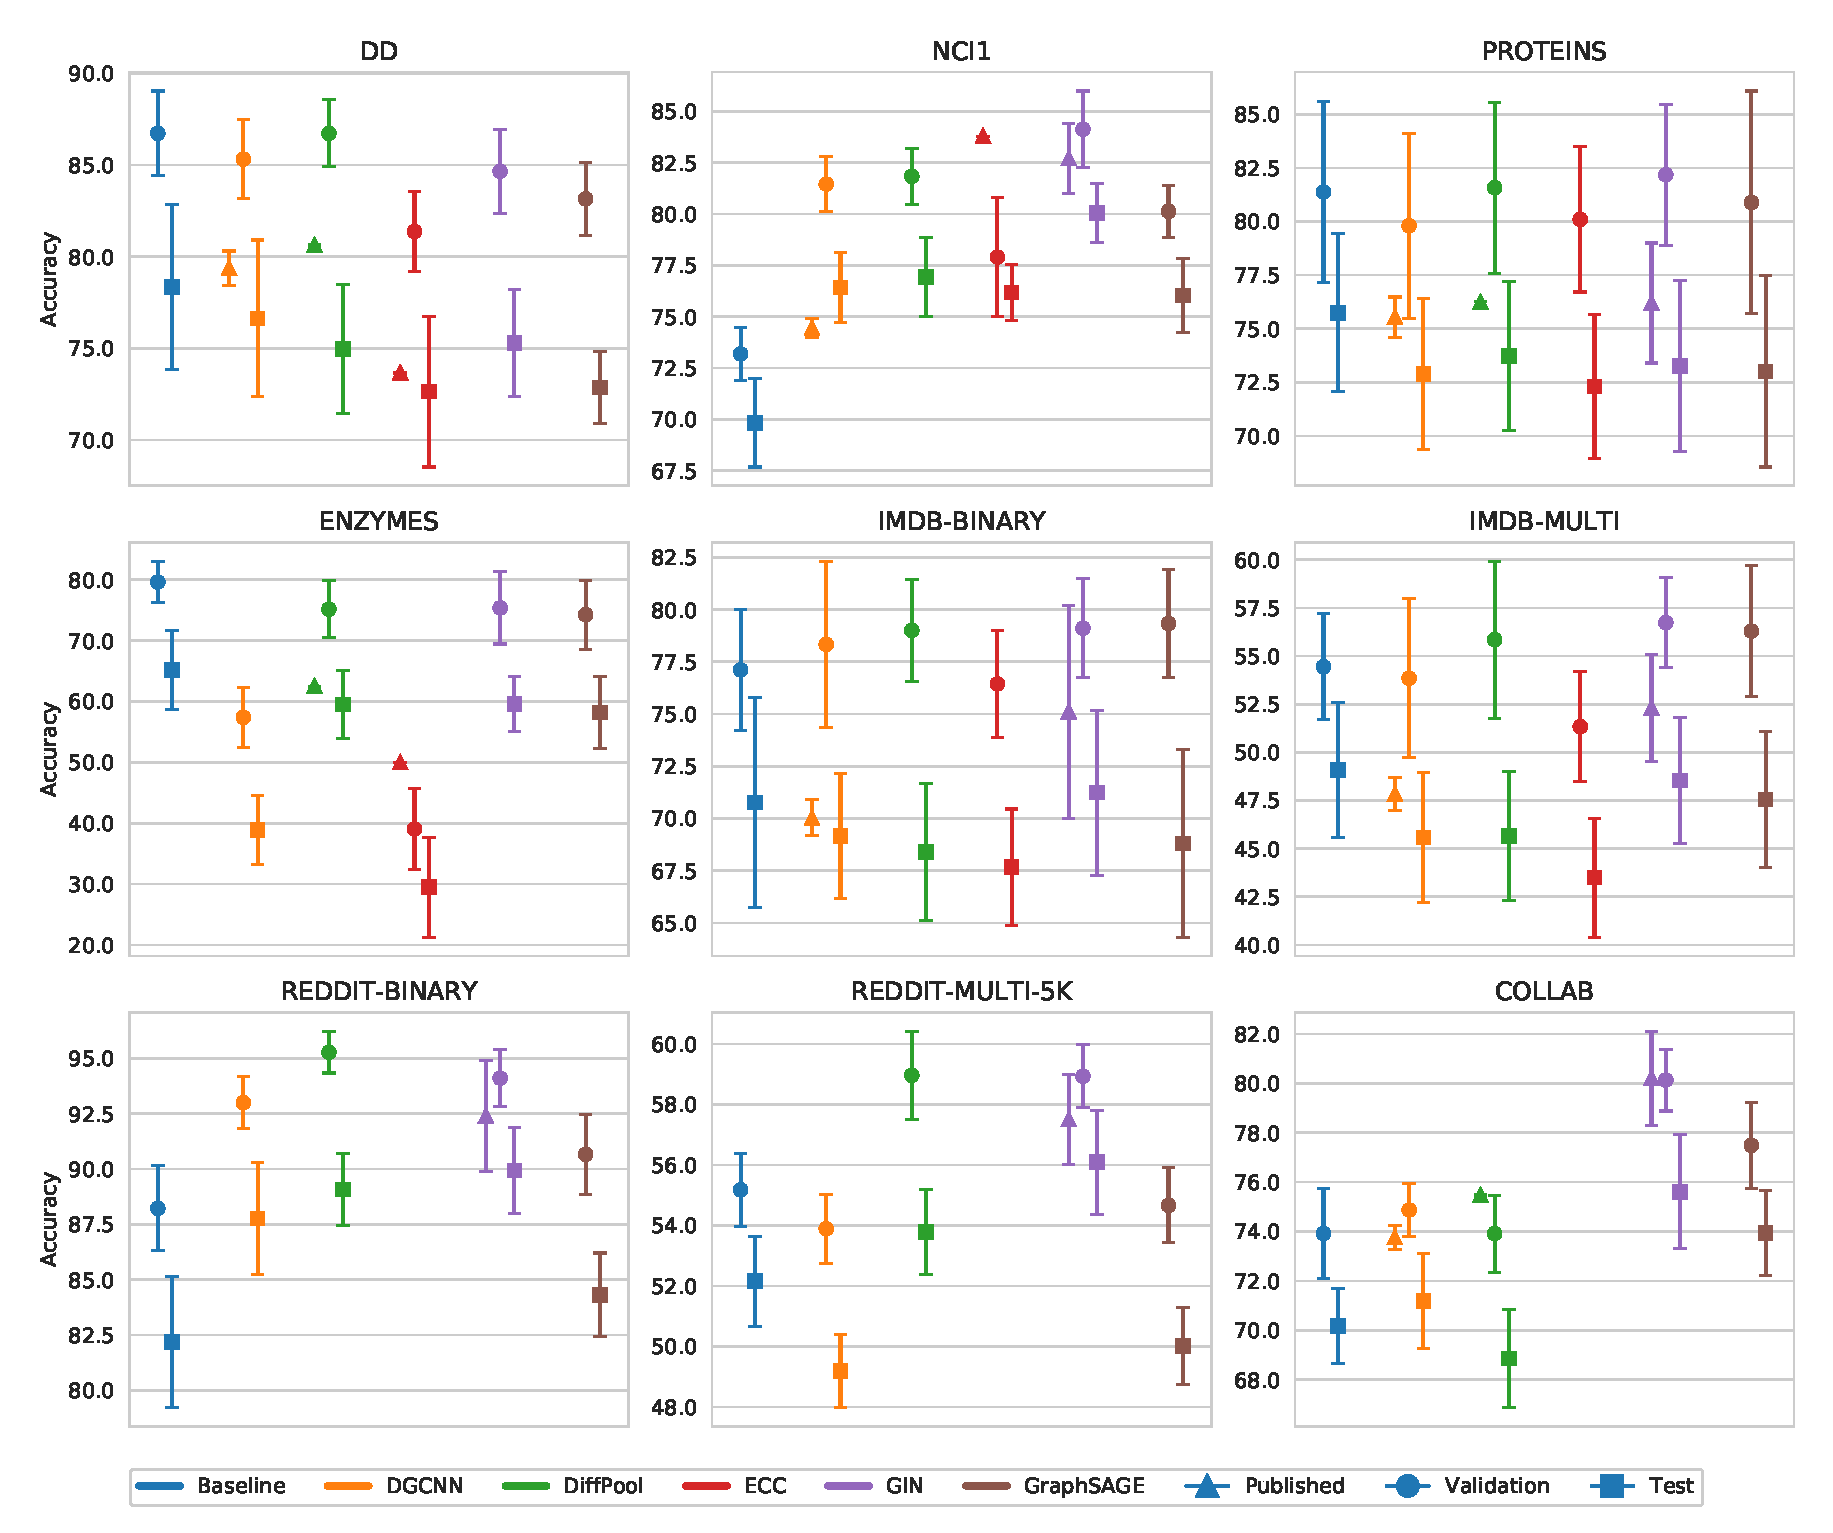
\includegraphics[width=\linewidth]{Figures/Chapter4/07-comparison-results.eps}
    \caption{Results.}
    \label{fig:comparison-plot}
\end{figure}

\section{Conclusions}
In this section, we showed how a rigorous empirical evaluation of \glspl{dgn} can help to design better experiments, and to draw more informed conclusions as regards the potential impact of novel architectures. This has been possible by introducing a clear and reproducible environment for benchmarking current and future \gls{dgn} architectures, as well as with reliable and reproducible results to which \gls{dgn} practitioners can test novel architectures. This work will hopefully prove useful to researchers and practitioners that want to compare \glspl{dgn} in a more rigorous way.

\chapter{Case Study: Prediction of Dynamical Properties of Biochemical Pathways using Deep Graph Networks}\label{ch:prediction-biochemical-dgn}

In this chapter, we present an application of Deep Learning techniques on graphs to a life sciences problem related to computational biology. Specifically, we apply Deep Graph Networks to process biochemical pathways, \ie dynamical systems that model the complex interactions between molecules at the biochemical level. Biochemical pathways can be represented as a particular form of bipartite graphs known as Petri networks, which allow to study several properties of such systems. Here, we focus on the property of concentration robustness. To be measured, concentration robustness requires to perform time-expensive simulations. Here, we opt for an approximate but reliable solution, which is orders of magnitude faster to compute. Through processing of the Petri network associated to the biochemical pathway with Deep Graph Networks, we show experimentally that it is possible to build a model that predicts concentration robustness rapidly and with a satisfactory level of accuracy.

\section{Introduction and Motivation}
In order to understand the mechanisms underlying the functioning of living cells, it is necessary to analyze their activities at the biochemical level. Biochemical pathways (or pathways, in short) are complex dynamical systems in which molecules interact with each other through chemical reactions. In these reactions, molecules can take the role of reactant, product, promoter or inhibitor. The dynamics of a pathway are determined by the variation over time of the concentration of its molecules. To study these dynamics, two methodologies are traditionally employed. One consists in modelling the pathway as a system of \glspl{ode}, derived from the application of chemical kinetics laws such as the law of mass action. In cases where pathways involve molecules available in small concentrations, which make the dynamics of reactions sensitive to random events, stochastic modelling and simulation approaches are preferred. These are usually variants of the well-known Gillespie's simulation algorithm \citep{gillespie1977exact}. The use of these modelling tools allows to investigate dynamical properties of biochemical pathways such as the reachability of steady states, the occurrence of oscillatory behaviors, causalities between molecular species, and robustness. However, quantitatively measuring these properties often requires to execute a large number of numerical or stochastic simulation, which in turn are time-consuming and computationally intensive.

Given their nature, one widely used formalism to represent biochemical pathways is that of graphs. Many different graphical notations of pathways exist in the literature (see, e.g., \citet{karp1994representations,reddy1993petri,le2009systems}), most of which represent molecules as nodes, and reactions as multi-edges or as additional nodes. Using graphs to represent pathways is convenient for three main reasons. Firstly, they provide a quite natural visual representation of the reactions occurring in the pathway. Secondly, they enable the study of the pathway dynamics through methods such as network and structural analysis. Thirdly, graphs can easily be transformed into \glspl{ode} or stochastic models, to apply standard numerical simulation techniques.

In this study, we investigate whether predicting dynamical properties of biochemical pathways from the structure of their associated graphs is possible; and if so, to what extent. In other words, our main assumption is that the dynamics of the biological system modeled by the pathway can be correlated to the structural properties of the graph by which it is represented. If the assumption is correct, the positive implications are two-fold: on one hand, a good predictive model of desired biochemical properties could, in principle, replace numerical or stochastic simulations whenever time and computational budgets are limited. On the other hand, it could allow to predict the properties even in cases where the quantitative information is not available, for example whenever numerical or stochastic simulation methods cannot be applied.

The main idea behind this work is to use of Deep Graph Networks to learn structural features of pathways represented as Petri networks (or Petri nets, in short), which are used to predict a property of interest. Here, we focus on the assessment of the dynamical property of robustness, defined as the the ability of a pathway to preserve its dynamics despite the perturbation of some parameters or initial conditions. More specifically, given a pathway and a pair of molecular species (called \emph{input} and \emph{output} species), the robustness measures how much the concentration of the output species at the steady state is influenced by perturbations of the initial concentration of the input species. This is a notion of \emph{concentration robustness} \citep{kitano2004biological} which is to some extent correlated with the notion of global sensitivity \citep{zi2011sensitivity}. Robustness makes up for a perfect candidate to test our approach, as its assessment is time-consuming and computationally intensive, requiring a huge number of simulations to explore the parameters space.

The initial part of this work focuses on the creation of a dataset suited to train the \gls{dgn}. We start from collecting 706 curated pathway models in SBML format from the BioModels\footnote{BioModels: \url{https://www.ebi.ac.uk/biomodels/}} database \citep{BioModels2010}, which were initially converted into Petri nets. For every pathway in this initial dataset, the robustness of every possible pair of input and output species has been computed through \gls{ode}-based simulations. Then, these robustness values have been transformed into binary indicators of whether robustness holds for a given pathway and input/output species. Lastly, for each pathway and for each input/output species in that pathway, the induced subgraphs containing the input and output nodes (as well as other nodes that influence the pathway dynamics) have been extracted. To summarize, the final dataset obtained with this preparatory phase consists of a set of subgraphs, each associated to a pair of input/output molecular species, and their respective robustness indicator. The predictive task is thus one of binary classification: specifically, given a subgraph and two nodes corresponding to the input and output species, the model should correctly classify them as robust or not.

We model the task with a \gls{dgn} to learn structural features from the subgraphs and compute a graph embedding that is passed to a \gls{mlp} classifier. The performances of the model are assessed according to a rigorous framework similar to the one developed in \ref{sec:comparison-exp-setup}. Our experimental results show that we are indeed able to predict robustness with reasonable accuracy. We also conduct a follow-up investigation of how the architectural choices, such as type of graph convolutional layer and number of layer, impact performances. The analysis suggests that the depth of the \gls{dgn}, in terms of number of layers, plays an important role in capturing the right features that correlate the subgraph structure to the robustness, and that deep \glspl{dgn} perform better at this task.

To our knowledge, this is the first work that addresses the problem of predicting dynamical, properties of pathways on a large scale using Deep Learning. In contrast, other approaches in the literature mainly focus on inferring the parameters of a single pathway, or the relationships between its species. We believe this work has great potential in helping understand the functioning of living cells, by serving as a fast, and computationally friendlier, alternative to performing expensive simulations in the assessment of pathway properties.

\section{Background}\label{sect:background}
In this section, we provide the necessary formal background to understand the modeling of biochemical pathways with Petri nets, and the dynamical property of concentration robustness.

\subsection{Pathway Petri Nets}\label{sec:ppn}
Biochemical pathways are essentially sets of chemical reactions of the form:
\[
c_1 S_1 + c_2 S_2 + \ldots
\xrightarrow{k}
c_1' P_1 + c_2' P_2 \ldots,
\]
where $S_i,P_i$ are molecules (\emph{reactants} and \emph{products}, respectively), $c_i, c_i' \in \Natural$ are \emph{stoichiometric coefficients} expressing the multiplicities of reactants and products involved in the reaction, and $k \in \Real_{\geq 0}$ is the \emph{kinetic constant}, used to compute the reaction rate according to standard chemical kinetic laws such as the law of mass action. Besides reactants and products, the reactions of a biochemical pathway often include in their description other molecules, called \emph{modifiers}. These are not consumed nor produced by the reaction, but act either as \emph{promoters} or as \emph{inhibitors}, meaning that they can increase or decrease the reaction rate, respectively. Although these molecules are not listed among reactants and products, they do have a role in the kinetic formula, which no longer follows the mass action principle in this case. For example, in the SBML language \citep{hucka2018sbml}, a standard XML-based modeling language for biochemical pathways, reactions can be associated with a number of modifiers, whose concentration is used in the kinetic formula of the reaction. In Figure \ref{subfig:example-reactions} we show a table describing the set of reactions describing a biochemical pathway (first column), some of which include a modifier (second column), namely $A$ for the third reaction, and $F$ for the sixth. Each reaction is associated with its kinetic formula (third column), that, for simplicity, we reference through an alias of the form $\mathsf{r}i$ with $i = 1, \ldots, 7$. Using the kinetic formulas of the two reactions with modifiers as an example, it is clear that $A$ acts as a promoter (meaning that the reaction rate is proportional to the concentration of $A$) and that $F$ acts as inhibitor (meaning that the reaction rate is inversely proportional to the concentration of $F$). Kinetic formulas can then be used to construct a system of \glspl{ode} as shown in Figure \ref{subfig:example-odes}.

\begin{figure}
\begin{subfigure}[b]{0.49\linewidth}
    \[\def\arraystretch{1.2}
    \begin{array}{ccl}
      \mbox{Reaction } & \mbox{ Modifiers } & \mbox{ Kinetics}\\
      \hline
      \SF{A} + \SF{B} \rightarrow 2\SF{B} &      & \SF{r}1 = k_1\SF{AB}\\
      \SF{B} \rightarrow \SF{A}      &      & \SF{r}2 = k_2\SF{B}\\
      \SF{C} + \SF{D} \rightarrow \SF{E}  & \SF{A}    & \SF{r}3 = k_3\SF{CDA}\\
      \SF{E} \rightarrow \SF{F}      &      & \SF{r}4 = k_4\SF{E}\\
      \SF{F} \rightarrow \SF{E}      &      & \SF{r}5 = k_5\SF{F}\\
      \SF{G} \rightarrow \SF{H}      & \SF{F}    & \SF{r}6 = \frac{k_6\SF{G}}{1+2 \SF{F}}\\
      \SF{H} \rightarrow \SF{G}      &      & \SF{r}7 = k_7\SF{H}\\
    \end{array}
    \]
\caption{Reactions}\label{subfig:example-reactions}
\end{subfigure}
%
\begin{subfigure}[b]{0.49\linewidth}
\[\def\arraystretch{1.2}
\begin{array}{l}
    \frac{d\SF{A}}{dt} = -k_1\SF{A}B + k_2\SF{B}\\
    \frac{d\SF{B}}{dt} = k_1\SF{AB} - k_2\SF{B}\\
    \frac{d\SF{C}}{dt} = -k_3\SF{CDA}\\
    \frac{d\SF{D}}{dt} = -k_3\SF{CDA}\\
    \frac{d\SF{E}}{dt} = k_3\SF{CDA} - k_4\SF{E} + k_5\SF{F}\\
    \frac{d\SF{F}}{dt} = k_4\SF{E} - k_5\SF{F}\\
    \frac{d\SF{G}}{dt} = -\frac{k_6\SF{G}}{1+2 \SF{F}} + k_7\SF{H}\\
    \frac{d\SF{H}}{dt} = \frac{k_6\SF{G}}{1+2 \SF{F}} - k_7\SF{H}
\end{array}
\]
\caption{ODEs}\label{subfig:example-odes}
\end{subfigure}
%
\caption{An example of biochemical pathway. ({\scriptsize A}) list of reactions with information on modifiers and kinetic formulas. ({\scriptsize B}) the corresponding system of ODEs.}\label{fig:example-pathway}
\end{figure}

A common way to represent biochemical pathways is through Petri nets \citep{?}. The formalism of Petri nets have been originally proposed for the description and analysis of concurrent systems \citep{peterson1977petri}, but has been later adopted to model other kinds of systems, such as biological ones. Several variants of Petri nets have been proposed in the literature. In this work, we consider a version of \emph{continuous} Petri nets \citep{gilbert2007petri} with promotion and inhibition edges and general kinetic functions. We call this biologically inspired variant \gls{ppn}. A \gls{ppn} is essentially a bipartite graph with two types of nodes and three types of labelled edges. According to standard Petri nets terminology, the two types of nodes are called \emph{places} and \emph{transitions}. The semantics of a \gls{ppn} in a continuous setting are described by a system of ODEs, with one equation for each place. In the case of pathways, such system corresponds exactly to the one obtained from the chemical reactions shown in Figure \ref{subfig:example-odes}. The state of a \gls{ppn} (called \emph{marking}) is then defined as an assignment of positive real values to the variables of the ODEs. We denote with $\Cal{M}$ the set of all possible markings.

More formally, a \gls{ppn} can be defined as a tuple $\wp = \Tuple{\Cal{P},\Cal{T},\Cal{A}_{S}, \Cal{A}_{P},\Cal{A}_{I},\vartheta,\varsigma,M_0}$ where:
\begin{itemize}
    \item $\Cal{P}$ and $\Cal{T}$ are finite, non empty disjoint sets of places and transitions, respectively;
    \item $\Cal{A}_{S} = ((\Cal{P}\times \Cal{T}) \cup (\Cal{T}\times \Cal{P})$ is a set of standard directed edges;
    \item $\Cal{A}_{P} \subseteq (\Cal{P} \times \Cal{T})$ is the set of promotion edges;
    \item $\Cal{A}_{I} \subseteq (\Cal{P} \times \Cal{T})$ is the set of inhibition edges;
    \item $\varsigma: \Cal{A}_{S} \shortrightarrow \mathbb{N}^{\geq 0}$ weights every standard edge by non-negative integer values;
    \item $\varsigma:\Cal{T} \shortrightarrow (\Cal{M} \rightarrow \mathbb{R}^{\geq 0})$,  is a function that assigns, to each transition, a function that computes a kinetic formula to every possible marking $M \in \Cal{M}$;
    \item $M_0 \in \Cal{M}$ is the initial marking.
\end{itemize}
A visual representation of the \gls{ppn} corresponding to the pathway in Figure \ref{subfig:example-reactions} is shown in Figure \ref{subfig:pathway-petri-net}. The sets of places $\Cal{P}$ and transitions $\Cal{T}$ of a pathway Petri net represent molecular species and reactants, and are displayed as circles and rectangles, respectively. In the figure, places are labeled with the name of the corresponding molecule. The directed edges, depicted as standard arrows, connect reactants to reactions and reactions to products. The weights of the edges (omitted if equal to one) correspond to the stoichiometric coefficients of reactant/product pairs. The sets of promotion and inhibition edges, $\Cal{A}_{P}$ and $\Cal{A}_{I}$, connect molecules to the reactions they promote or inhibit, respectively, and they are displayed as dotted or T-shaped arrows, respectively. The kinetic formulas of reactions (or rather, their aliases defined as in Figure \ref{subfig:pathway-petri-net}), are shown inside the rectangles of the corresponding transitions. As explained previously, molecules connected through promotion edges give a positive contribution to the value of the kinetic formula, while molecules connected through inhibition edges give a negative (inversely proportional) contribution. Finally, the initial marking $M_0$ is not shown in the figure, and it has to be described separately.
\begin{figure*}[h!]
    \centering
    \resizebox{.6\textwidth}{!}{

\tikzset{every picture/.style={line width=0.75pt}} %set default line width to 0.75pt        

\begin{tikzpicture}[x=0.75pt,y=0.75pt,yscale=-1,xscale=1]
%uncomment if require: \path (0,300); %set diagram left start at 0, and has height of 300

%Straight Lines [id:da3576438741903769] 
\draw    (388,210) -- (414.13,177.34) ;
\draw [shift={(416,175)}, rotate = 488.66] [fill={rgb, 255:red, 0; green, 0; blue, 0 }  ][line width=0.08]  [draw opacity=0] (8.93,-4.29) -- (0,0) -- (8.93,4.29) -- cycle    ;
%Straight Lines [id:da5206527388854192] 
\draw    (350,164) -- (376.13,196.66) ;
\draw [shift={(378,199)}, rotate = 231.34] [fill={rgb, 255:red, 0; green, 0; blue, 0 }  ][line width=0.08]  [draw opacity=0] (8.93,-4.29) -- (0,0) -- (8.93,4.29) -- cycle    ;
%Straight Lines [id:da9664135693242828] 
\draw    (388,110) -- (361.87,142.66) ;
\draw [shift={(360,145)}, rotate = 308.65999999999997] [fill={rgb, 255:red, 0; green, 0; blue, 0 }  ][line width=0.08]  [draw opacity=0] (8.93,-4.29) -- (0,0) -- (8.93,4.29) -- cycle    ;
%Straight Lines [id:da3150124855239005] 
\draw    (426,156) -- (399.87,123.34) ;
\draw [shift={(398,121)}, rotate = 411.34000000000003] [fill={rgb, 255:red, 0; green, 0; blue, 0 }  ][line width=0.08]  [draw opacity=0] (8.93,-4.29) -- (0,0) -- (8.93,4.29) -- cycle    ;
%Straight Lines [id:da2531638133399581] 
\draw    (295,160) -- (335,160) ;
%Straight Lines [id:da7978054588524539] 
\draw    (110,160) -- (157,160) ;
\draw [shift={(160,160)}, rotate = 180] [fill={rgb, 255:red, 0; green, 0; blue, 0 }  ][line width=0.08]  [draw opacity=0] (8.93,-4.29) -- (0,0) -- (8.93,4.29) -- cycle    ;
%Straight Lines [id:da5621074466789615] 
\draw    (235,125) -- (279.4,150.51) ;
\draw [shift={(282,152)}, rotate = 209.88] [fill={rgb, 255:red, 0; green, 0; blue, 0 }  ][line width=0.08]  [draw opacity=0] (8.93,-4.29) -- (0,0) -- (8.93,4.29) -- cycle    ;
%Straight Lines [id:da9432384230142636] 
\draw    (235,195) -- (190.6,169.49) ;
\draw [shift={(188,168)}, rotate = 389.88] [fill={rgb, 255:red, 0; green, 0; blue, 0 }  ][line width=0.08]  [draw opacity=0] (8.93,-4.29) -- (0,0) -- (8.93,4.29) -- cycle    ;
%Straight Lines [id:da2732887752012232] 
\draw    (295,160) -- (252.62,183.54) ;
\draw [shift={(250,185)}, rotate = 330.95] [fill={rgb, 255:red, 0; green, 0; blue, 0 }  ][line width=0.08]  [draw opacity=0] (8.93,-4.29) -- (0,0) -- (8.93,4.29) -- cycle    ;
%Straight Lines [id:da8361705783456022] 
\draw    (175,160) -- (217.38,136.46) ;
\draw [shift={(220,135)}, rotate = 510.95] [fill={rgb, 255:red, 0; green, 0; blue, 0 }  ][line width=0.08]  [draw opacity=0] (8.93,-4.29) -- (0,0) -- (8.93,4.29) -- cycle    ;
%Straight Lines [id:da26704871020062715] 
\draw    (110,90) -- (157.05,81.23) ;
\draw [shift={(160,80.68)}, rotate = 529.44] [fill={rgb, 255:red, 0; green, 0; blue, 0 }  ][line width=0.08]  [draw opacity=0] (8.93,-4.29) -- (0,0) -- (8.93,4.29) -- cycle    ;
%Straight Lines [id:da4846937260313433] 
\draw    (40,80.68) -- (87.05,89.45) ;
\draw [shift={(90,90)}, rotate = 190.56] [fill={rgb, 255:red, 0; green, 0; blue, 0 }  ][line width=0.08]  [draw opacity=0] (8.93,-4.29) -- (0,0) -- (8.93,4.29) -- cycle    ;
%Straight Lines [id:da271105016276878] 
\draw    (105,25) -- (157.47,58.39) ;
\draw [shift={(160,60)}, rotate = 212.47] [fill={rgb, 255:red, 0; green, 0; blue, 0 }  ][line width=0.08]  [draw opacity=0] (8.93,-4.29) -- (0,0) -- (8.93,4.29) -- cycle    ;
%Shape: Rectangle [id:dp9228181661849988] 
\draw  [fill={rgb, 255:red, 255; green, 255; blue, 255 }  ,fill opacity=1 ] (20,50) -- (50,50) -- (50,90) -- (20,90) -- cycle ;
%Straight Lines [id:da06467494297119436] 
\draw    (105,25) -- (52.53,58.39) ;
\draw [shift={(50,60)}, rotate = 327.53] [fill={rgb, 255:red, 0; green, 0; blue, 0 }  ][line width=0.08]  [draw opacity=0] (8.93,-4.29) -- (0,0) -- (8.93,4.29) -- cycle    ;
%Shape: Circle [id:dp49236484975772] 
\draw  [fill={rgb, 255:red, 255; green, 255; blue, 255 }  ,fill opacity=1 ] (90,25) .. controls (90,16.72) and (96.72,10) .. (105,10) .. controls (113.28,10) and (120,16.72) .. (120,25) .. controls (120,33.28) and (113.28,40) .. (105,40) .. controls (96.72,40) and (90,33.28) .. (90,25) -- cycle ;
%Shape: Rectangle [id:dp3146550401206405] 
\draw  [fill={rgb, 255:red, 255; green, 255; blue, 255 }  ,fill opacity=1 ] (160,50) -- (190,50) -- (190,90) -- (160,90) -- cycle ;
%Curve Lines [id:da9984566963389516] 
\draw    (190,70) .. controls (250.06,70.4) and (250.75,-32.96) .. (121.95,19.2) ;
\draw [shift={(120,20)}, rotate = 337.56] [fill={rgb, 255:red, 0; green, 0; blue, 0 }  ][line width=0.08]  [draw opacity=0] (8.93,-4.29) -- (0,0) -- (8.93,4.29) -- cycle    ;
%Shape: Circle [id:dp09345090103745823] 
\draw  [fill={rgb, 255:red, 255; green, 255; blue, 255 }  ,fill opacity=1 ] (90,95) .. controls (90,86.72) and (96.72,80) .. (105,80) .. controls (113.28,80) and (120,86.72) .. (120,95) .. controls (120,103.28) and (113.28,110) .. (105,110) .. controls (96.72,110) and (90,103.28) .. (90,95) -- cycle ;
%Straight Lines [id:da5223576478149881] 
\draw    (105,110) -- (105,131) ;
\draw [shift={(105,131)}, rotate = 90] [color={rgb, 255:red, 0; green, 0; blue, 0 }  ][fill={rgb, 255:red, 0; green, 0; blue, 0 }  ][line width=0.75]      (0, 0) circle [x radius= 3.35, y radius= 3.35]   ;
%Shape: Rectangle [id:dp25364205729175127] 
\draw  [fill={rgb, 255:red, 255; green, 255; blue, 255 }  ,fill opacity=1 ] (90,140) -- (120,140) -- (120,180) -- (90,180) -- cycle ;
%Straight Lines [id:da8084682726089965] 
\draw    (40,140.68) -- (87.05,149.45) ;
\draw [shift={(90,150)}, rotate = 190.56] [fill={rgb, 255:red, 0; green, 0; blue, 0 }  ][line width=0.08]  [draw opacity=0] (8.93,-4.29) -- (0,0) -- (8.93,4.29) -- cycle    ;
%Straight Lines [id:da8278541197200837] 
\draw    (40,180) -- (87.05,171.23) ;
\draw [shift={(90,170.68)}, rotate = 529.44] [fill={rgb, 255:red, 0; green, 0; blue, 0 }  ][line width=0.08]  [draw opacity=0] (8.93,-4.29) -- (0,0) -- (8.93,4.29) -- cycle    ;
%Shape: Circle [id:dp5697702501712039] 
\draw  [fill={rgb, 255:red, 255; green, 255; blue, 255 }  ,fill opacity=1 ] (20,137) .. controls (20,128.72) and (26.72,122) .. (35,122) .. controls (43.28,122) and (50,128.72) .. (50,137) .. controls (50,145.28) and (43.28,152) .. (35,152) .. controls (26.72,152) and (20,145.28) .. (20,137) -- cycle ;
%Shape: Circle [id:dp027027959729662543] 
\draw  [fill={rgb, 255:red, 255; green, 255; blue, 255 }  ,fill opacity=1 ] (20,183) .. controls (20,174.72) and (26.72,168) .. (35,168) .. controls (43.28,168) and (50,174.72) .. (50,183) .. controls (50,191.28) and (43.28,198) .. (35,198) .. controls (26.72,198) and (20,191.28) .. (20,183) -- cycle ;
%Shape: Circle [id:dp7929646959402241] 
\draw  [fill={rgb, 255:red, 255; green, 255; blue, 255 }  ,fill opacity=1 ] (160,160) .. controls (160,151.72) and (166.72,145) .. (175,145) .. controls (183.28,145) and (190,151.72) .. (190,160) .. controls (190,168.28) and (183.28,175) .. (175,175) .. controls (166.72,175) and (160,168.28) .. (160,160) -- cycle ;
%Shape: Rectangle [id:dp05655391624383377] 
\draw  [fill={rgb, 255:red, 255; green, 255; blue, 255 }  ,fill opacity=1 ] (220,115) -- (250,115) -- (250,155) -- (220,155) -- cycle ;
%Shape: Rectangle [id:dp05796590340987029] 
\draw  [fill={rgb, 255:red, 255; green, 255; blue, 255 }  ,fill opacity=1 ] (220,165) -- (250,165) -- (250,205) -- (220,205) -- cycle ;
%Shape: Circle [id:dp13273124949760895] 
\draw  [fill={rgb, 255:red, 255; green, 255; blue, 255 }  ,fill opacity=1 ] (280,160) .. controls (280,151.72) and (286.72,145) .. (295,145) .. controls (303.28,145) and (310,151.72) .. (310,160) .. controls (310,168.28) and (303.28,175) .. (295,175) .. controls (286.72,175) and (280,168.28) .. (280,160) -- cycle ;
%Straight Lines [id:da9347007050049654] 
\draw    (335.29,154.43) -- (335.26,165.81) ;
%Straight Lines [id:da20553639689795267] 
\draw    (336,154.43) -- (335.97,165.81) ;
%Shape: Rectangle [id:dp30165349356224813] 
\draw  [fill={rgb, 255:red, 255; green, 255; blue, 255 }  ,fill opacity=1 ] (380,145) -- (380,175) -- (340,175) -- (340,145) -- cycle ;
%Shape: Rectangle [id:dp05448702121100979] 
\draw  [fill={rgb, 255:red, 255; green, 255; blue, 255 }  ,fill opacity=1 ] (436,145) -- (436,175) -- (396,175) -- (396,145) -- cycle ;
%Shape: Circle [id:dp37659499504730287] 
\draw  [fill={rgb, 255:red, 255; green, 255; blue, 255 }  ,fill opacity=1 ] (373,110) .. controls (373,101.72) and (379.72,95) .. (388,95) .. controls (396.28,95) and (403,101.72) .. (403,110) .. controls (403,118.28) and (396.28,125) .. (388,125) .. controls (379.72,125) and (373,118.28) .. (373,110) -- cycle ;
%Shape: Circle [id:dp13055596917815526] 
\draw  [fill={rgb, 255:red, 255; green, 255; blue, 255 }  ,fill opacity=1 ] (373,210) .. controls (373,201.72) and (379.72,195) .. (388,195) .. controls (396.28,195) and (403,201.72) .. (403,210) .. controls (403,218.28) and (396.28,225) .. (388,225) .. controls (379.72,225) and (373,218.28) .. (373,210) -- cycle ;

% Text Node
\draw (26,62) node [anchor=north west][inner sep=0.75pt]   [align=left] {$\mathsf{r2}$};
% Text Node
\draw (168,62) node [anchor=north west][inner sep=0.75pt]   [align=left] {$\mathsf{r1}$};
% Text Node
\draw (97,153) node [anchor=north west][inner sep=0.75pt]   [align=left] {$\mathsf{r3}$};
% Text Node
\draw (227,127) node [anchor=north west][inner sep=0.75pt]   [align=left] {$\mathsf{r4}$};
% Text Node
\draw (227,178) node [anchor=north west][inner sep=0.75pt]   [align=left] {$\mathsf{r5}$};
% Text Node
\draw (352,154) node [anchor=north west][inner sep=0.75pt]   [align=left] {$\mathsf{r6}$};
% Text Node
\draw (409,154) node [anchor=north west][inner sep=0.75pt]   [align=left] {$\mathsf{r7}$};

% Text Node
\draw (98,18) node [anchor=north west][inner sep=0.75pt]   [align=left] {$\mathsf{B}$};
% Text Node
\draw (98,89) node [anchor=north west][inner sep=0.75pt]   [align=left] {$\mathsf{A}$};
% Text Node
\draw (28,130) node [anchor=north west][inner sep=0.75pt]   [align=left] {$\mathsf{C}$};
% Text Node
\draw (28,177) node [anchor=north west][inner sep=0.75pt]   [align=left] {$\mathsf{D}$};
% Text Node
\draw (168,153) node [anchor=north west][inner sep=0.75pt]   [align=left] {$\mathsf{E}$};
% Text Node
\draw (289,153) node [anchor=north west][inner sep=0.75pt]   [align=left] {$\mathsf{F}$};
% Text Node
\draw (381,103) node [anchor=north west][inner sep=0.75pt]   [align=left] {$\mathsf{G}$};
% Text Node
\draw (381,203) node [anchor=north west][inner sep=0.75pt]   [align=left] {$\mathsf{H}$};
% Text Node
\draw (232,24) node [anchor=north west][inner sep=0.75pt]   [align=left] {$\mathsf{2}$};


\end{tikzpicture}}
    \caption{The Pathway Petri Net corresponding to the reactions described in Figure \ref{subfig:example-reactions}}
    \label{subfig:pathway-petri-net}
\end{figure*}

In this work, we use a variant of \glspl{ppn} where all the information unrelated to the structure of the pathway is discarded. Specifically, we ignore information about:
\begin{itemize}
    \item kinetic formulas;
    \item multiplicities of reactants and products (\ie edge labels);
    \item the initial marking $M_0$.
\end{itemize}
Basically, for our purposes, a \gls{ppn} is a tuple $\wp = \Tuple{\Cal{P},\Cal{T},\Cal{A}_{S}, \Cal{A}_{P},\Cal{A}_{I}}$ where the irrelevant components have been omitted. We rewrite this object, according to the graph notation introduced in Section \ref{sec:graphs}, into a \keyword{pathway graph} $G = \Tuple{\Cal{V}_G, \Cal{E}_G}$. To do so, we first define the following nodes and edges subsets:
\begin{itemize}
    \item $\Cal{V}_{G}^{\Fun{mol}} = \Cal{P}$ is the set of molecules;
    \item $\Cal{V}_{G}^{\Fun{rx}} = \Cal{T}$ is the set of reactions;
    \item $\Cal{E}_{G}^{\Fun{std}} = \Cal{A}_S$ is the set of standard edges;
    \item $\Cal{E}_{G}^{\Fun{pro}} = \Cal{A}_P$ is the set of promoter edges;
    \item $\Cal{E}_{G}^{\Fun{inh}} = \Cal{A}_I$ is the set of inhibitor edges,
\end{itemize}
where $\Cal{V}_{G}^{\Fun{mol}} \Inter \Cal{V}_{G}^{\Fun{rx}} = \emptyset$ and $\Cal{E}_{G}^{\Fun{std}} \Inter \Cal{E}_{G}^{\Fun{pro}} \Inter \Cal{E}_{G}^{\Fun{inh}} = \emptyset$. Then, we simply set $\Cal{V}_G = \Cal{V}_G^{\Fun{mol}} \Union \Cal{V}_G^{\Fun{rx}}$ and $\Cal{E}_G = \Cal{E}_G^{\Fun{std}} \Union \Cal{E}_G^{\Fun{pro}} \Union \Cal{E}_G^{\Fun{inh}}$.
Using the biochemical pathway of Figure \ref{fig:example-pathway} as reference, its associated pathway graph is shown in Figure \ref{fig:pathway-graph}.
\begin{figure*}[h!]
    \centering
    \resizebox{.6\textwidth}{!}{

\tikzset{every picture/.style={line width=0.75pt}} %set default line width to 0.75pt

\begin{tikzpicture}[x=0.75pt,y=0.75pt,yscale=-1,xscale=1]
%uncomment if require: \path (0,300); %set diagram left start at 0, and has height of 300

%Straight Lines [id:da289255485986883]
\draw    (100,56) -- (135.62,83.18) ;
\draw [shift={(138,85)}, rotate = 217.35] [fill={rgb, 255:red, 0; green, 0; blue, 0 }  ][line width=0.08]  [draw opacity=0] (5.36,-2.57) -- (0,0) -- (5.36,2.57) -- cycle    ;

% Text Node
\draw  [fill={rgb, 255:red, 255; green, 255; blue, 255 }  ,fill opacity=1 ]  (38,78) -- (62,78) -- (62,112) -- (38,112) -- cycle  ;
\draw (50,95) node   [align=left] {\begin{minipage}[lt]{13.600000000000001pt}\setlength\topsep{0pt}
\begin{center}
\end{center}

\end{minipage}};
% Text Node
\draw  [fill={rgb, 255:red, 255; green, 255; blue, 255 }  ,fill opacity=1 ]  (100, 55.5) circle [x radius= 13.2, y radius= 13.2]   ;
\draw (100,55.5) node   [align=left] {\begin{minipage}[lt]{14.96pt}\setlength\topsep{0pt}
\begin{center}
\SF{B}
\end{center}

\end{minipage}};
% Text Node
\draw  [fill={rgb, 255:red, 255; green, 255; blue, 255 }  ,fill opacity=1 ]  (138,78) -- (162,78) -- (162,112) -- (138,112) -- cycle  ;
\draw (150,95) node   [align=left] {\begin{minipage}[lt]{13.600000000000001pt}\setlength\topsep{0pt}
\begin{center}
\end{center}

\end{minipage}};
% Text Node
\draw  [fill={rgb, 255:red, 255; green, 255; blue, 255 }  ,fill opacity=1 ]  (100, 135.5) circle [x radius= 13.2, y radius= 13.2]   ;
\draw (100,135.5) node   [align=left] {\begin{minipage}[lt]{14.96pt}\setlength\topsep{0pt}
\begin{center}
\SF{A}
\end{center}

\end{minipage}};
% Text Node
\draw  [fill={rgb, 255:red, 255; green, 255; blue, 255 }  ,fill opacity=1 ]  (39, 175.5) circle [x radius= 13.2, y radius= 13.2]   ;
\draw (39,175.5) node   [align=left] {\begin{minipage}[lt]{14.96pt}\setlength\topsep{0pt}
\begin{center}
\SF{C}
\end{center}

\end{minipage}};
% Text Node
\draw  [fill={rgb, 255:red, 255; green, 255; blue, 255 }  ,fill opacity=1 ]  (39, 215.5) circle [x radius= 13.2, y radius= 13.2]   ;
\draw (39,215.5) node   [align=left] {\begin{minipage}[lt]{14.96pt}\setlength\topsep{0pt}
\begin{center}
\SF{D}
\end{center}

\end{minipage}};
% Text Node
\draw  [fill={rgb, 255:red, 255; green, 255; blue, 255 }  ,fill opacity=1 ]  (88,178) -- (112,178) -- (112,212) -- (88,212) -- cycle  ;
\draw (100,195) node   [align=left] {\begin{minipage}[lt]{13.600000000000001pt}\setlength\topsep{0pt}
\begin{center}
\end{center}

\end{minipage}};
% Text Node
\draw  [fill={rgb, 255:red, 255; green, 255; blue, 255 }  ,fill opacity=1 ]  (159, 195.5) circle [x radius= 13.2, y radius= 13.2]   ;
\draw (159,195.5) node   [align=left] {\begin{minipage}[lt]{14.96pt}\setlength\topsep{0pt}
\begin{center}
\SF{E}
\end{center}

\end{minipage}};
% Text Node
\draw  [fill={rgb, 255:red, 255; green, 255; blue, 255 }  ,fill opacity=1 ]  (198,148) -- (222,148) -- (222,182) -- (198,182) -- cycle  ;
\draw (210,165) node   [align=left] {\begin{minipage}[lt]{13.600000000000001pt}\setlength\topsep{0pt}
\begin{center}
\end{center}

\end{minipage}};
% Text Node
\draw  [fill={rgb, 255:red, 255; green, 255; blue, 255 }  ,fill opacity=1 ]  (198,208) -- (222,208) -- (222,242) -- (198,242) -- cycle  ;
\draw (210,225) node   [align=left] {\begin{minipage}[lt]{13.600000000000001pt}\setlength\topsep{0pt}
\begin{center}
\end{center}

\end{minipage}};
% Text Node
\draw  [fill={rgb, 255:red, 255; green, 255; blue, 255 }  ,fill opacity=1 ]  (269, 195.5) circle [x radius= 13.2, y radius= 13.2]   ;
\draw (269,195.5) node   [align=left] {\begin{minipage}[lt]{14.96pt}\setlength\topsep{0pt}
\begin{center}
\SF{F}
\end{center}

\end{minipage}};
% Text Node
\draw  [fill={rgb, 255:red, 255; green, 255; blue, 255 }  ,fill opacity=1 ]  (318,183) -- (352,183) -- (352,207) -- (318,207) -- cycle  ;
\draw (335,195) node   [align=left] {\begin{minipage}[lt]{20.400000000000002pt}\setlength\topsep{0pt}
\begin{center}
\end{center}

\end{minipage}};
% Text Node
\draw  [fill={rgb, 255:red, 255; green, 255; blue, 255 }  ,fill opacity=1 ]  (398,183) -- (432,183) -- (432,207) -- (398,207) -- cycle  ;
\draw (415,195) node   [align=left] {\begin{minipage}[lt]{20.400000000000002pt}\setlength\topsep{0pt}
\begin{center}
\end{center}

\end{minipage}};
% Text Node
\draw  [fill={rgb, 255:red, 255; green, 255; blue, 255 }  ,fill opacity=1 ]  (374, 155.5) circle [x radius= 13.2, y radius= 13.2]   ;
\draw (374,155.5) node   [align=left] {\begin{minipage}[lt]{14.96pt}\setlength\topsep{0pt}
\begin{center}
\SF{G}
\end{center}

\end{minipage}};
% Text Node
\draw  [fill={rgb, 255:red, 255; green, 255; blue, 255 }  ,fill opacity=1 ]  (374, 234.5) circle [x radius= 13.2, y radius= 13.2]   ;
\draw (374,234.5) node   [align=left] {\begin{minipage}[lt]{14.96pt}\setlength\topsep{0pt}
\begin{center}
\SF{H}
\end{center}

\end{minipage}};
% Connection
\draw    (89.64,63.68) -- (64.35,83.66) ;
\draw [shift={(62,85.52)}, rotate = 321.69] [fill={rgb, 255:red, 0; green, 0; blue, 0 }  ][line width=0.08]  [draw opacity=0] (5.36,-2.57) -- (0,0) -- (5.36,2.57) -- cycle    ;
% Connection
\draw    (62,104.72) -- (87.41,125.3) ;
\draw [shift={(89.74,127.19)}, rotate = 219.01] [fill={rgb, 255:red, 0; green, 0; blue, 0 }  ][line width=0.08]  [draw opacity=0] (5.36,-2.57) -- (0,0) -- (5.36,2.57) -- cycle    ;
% Connection
\draw    (110.26,127.19) -- (135.67,106.61) ;
\draw [shift={(138,104.72)}, rotate = 500.99] [fill={rgb, 255:red, 0; green, 0; blue, 0 }  ][line width=0.08]  [draw opacity=0] (5.36,-2.57) -- (0,0) -- (5.36,2.57) -- cycle    ;
% Connection
\draw    (100,148.7) -- (100,173) ;
\draw [shift={(100,173)}, rotate = 90] [color={rgb, 255:red, 0; green, 0; blue, 0 }  ][fill={rgb, 255:red, 0; green, 0; blue, 0 }  ][line width=0.75]      (0, 0) circle [x radius= 3.35, y radius= 3.35]   ;
% Connection
\draw    (162,89.03) .. controls (203.8,73.44) and (164.07,35.95) .. (114.99,51.28) ;
\draw [shift={(112.74,52.02)}, rotate = 341.03] [fill={rgb, 255:red, 0; green, 0; blue, 0 }  ][line width=0.08]  [draw opacity=0] (5.36,-2.57) -- (0,0) -- (5.36,2.57) -- cycle    ;
% Connection
\draw    (51.58,179.52) -- (85.14,190.25) ;
\draw [shift={(88,191.16)}, rotate = 197.73] [fill={rgb, 255:red, 0; green, 0; blue, 0 }  ][line width=0.08]  [draw opacity=0] (5.36,-2.57) -- (0,0) -- (5.36,2.57) -- cycle    ;
% Connection
\draw    (51.52,211.29) -- (85.16,199.99) ;
\draw [shift={(88,199.03)}, rotate = 521.4200000000001] [fill={rgb, 255:red, 0; green, 0; blue, 0 }  ][line width=0.08]  [draw opacity=0] (5.36,-2.57) -- (0,0) -- (5.36,2.57) -- cycle    ;
% Connection
\draw    (112,195.1) -- (142.8,195.36) ;
\draw [shift={(145.8,195.39)}, rotate = 180.49] [fill={rgb, 255:red, 0; green, 0; blue, 0 }  ][line width=0.08]  [draw opacity=0] (5.36,-2.57) -- (0,0) -- (5.36,2.57) -- cycle    ;
% Connection
\draw    (170.33,188.72) -- (195.43,173.72) ;
\draw [shift={(198,172.18)}, rotate = 509.12] [fill={rgb, 255:red, 0; green, 0; blue, 0 }  ][line width=0.08]  [draw opacity=0] (5.36,-2.57) -- (0,0) -- (5.36,2.57) -- cycle    ;
% Connection
\draw    (222,171.2) -- (254.61,188.06) ;
\draw [shift={(257.27,189.44)}, rotate = 207.34] [fill={rgb, 255:red, 0; green, 0; blue, 0 }  ][line width=0.08]  [draw opacity=0] (5.36,-2.57) -- (0,0) -- (5.36,2.57) -- cycle    ;
% Connection
\draw    (257.19,201.4) -- (224.68,217.66) ;
\draw [shift={(222,219)}, rotate = 333.43] [fill={rgb, 255:red, 0; green, 0; blue, 0 }  ][line width=0.08]  [draw opacity=0] (5.36,-2.57) -- (0,0) -- (5.36,2.57) -- cycle    ;
% Connection
\draw    (198,218.06) -- (173.03,203.61) ;
\draw [shift={(170.43,202.11)}, rotate = 390.05] [fill={rgb, 255:red, 0; green, 0; blue, 0 }  ][line width=0.08]  [draw opacity=0] (5.36,-2.57) -- (0,0) -- (5.36,2.57) -- cycle    ;
% Connection
\draw    (282.2,195.4) -- (315,195.15) ;
\draw [shift={(315,195.15)}, rotate = 539.5699999999999] [color={rgb, 255:red, 0; green, 0; blue, 0 }  ][line width=0.75]    (0,5.59) -- (0,-5.59)   ;
% Connection
\draw    (346.85,207) -- (362.62,222.97) ;
\draw [shift={(364.73,225.11)}, rotate = 225.36] [fill={rgb, 255:red, 0; green, 0; blue, 0 }  ][line width=0.08]  [draw opacity=0] (5.36,-2.57) -- (0,0) -- (5.36,2.57) -- cycle    ;
% Connection
\draw    (383.51,225.34) -- (400.38,209.08) ;
\draw [shift={(402.54,207)}, rotate = 496.07] [fill={rgb, 255:red, 0; green, 0; blue, 0 }  ][line width=0.08]  [draw opacity=0] (5.36,-2.57) -- (0,0) -- (5.36,2.57) -- cycle    ;
% Connection
\draw    (402.54,183) -- (385.67,166.74) ;
\draw [shift={(383.51,164.66)}, rotate = 403.93] [fill={rgb, 255:red, 0; green, 0; blue, 0 }  ][line width=0.08]  [draw opacity=0] (5.36,-2.57) -- (0,0) -- (5.36,2.57) -- cycle    ;
% Connection
\draw    (364.73,164.89) -- (348.96,180.87) ;
\draw [shift={(346.85,183)}, rotate = 314.64] [fill={rgb, 255:red, 0; green, 0; blue, 0 }  ][line width=0.08]  [draw opacity=0] (5.36,-2.57) -- (0,0) -- (5.36,2.57) -- cycle    ;

\end{tikzpicture}}
    \caption{The pathway graph obtained by omitting kinetic formulas and edge labels from the one in Figure \ref{subfig:pathway-petri-net}. Notice that the names of the molecules are displayed for visual aid, but are not included of the pathway graph.}
    \label{fig:pathway-graph}
\end{figure*}
More explicitly, the set of nodes of the pathway graph contains both molecules and reactions. The set of edges of the graph contains an edge (of any type) from a molecule to a reaction if and only if a perturbation in the concentration of the molecule determines a change in the reaction rate (that could in principle be computed through the omitted kinetic formula). Similarly, it contains an edge from a reaction to a molecule if and only if a perturbation in the reaction rate determines a change in the dynamics of the concentration of that molecule. This is intuitive for those molecular species that are products, as the dynamics of the product accumulation is determined by the reaction rate. By construction, a pathway graph is bipartite.

\subsection{Concentration Robustness}\label{sec:robustness}
Robustness is defined as the ability of a system to maintain its functionalities again external and internal perturbations \citep{kitano2004biological}, a property observed in many biological systems. A general notion of robustness has been formalized by Kitano in \cite{kitano2007towards}. This formalization considers a specific functionality of a system and the \emph{viability} of such functionality, defined as the ability of the system (\eg a cell) to carry it out. This could be expressed, for instance, in terms of the synthesis/degradation rate or concentration level of some target substance, in terms of cell growth rate, or in terms of  other suitable quantitative indicators. More specifically, according to Kitano's definition, the robustness $R$ of a system $\mathbb{S}$, with respect to a specific functionality $a$ and against a set of perturbations $P$ is expressed as:
\[
 R^{\mathbb{S}}_{a,P} = \int_p \Psi(p) D_a^\mathbb{S}(p)dp
\]
In the above definition, $\Psi(p)$ is the probability a perturbation $p$, and $D_a(p)$ evaluates the functionality $a$ of the system $\mathbb{S}$ under the perturbation $p$. More precisely, function $D_a(p)$ gives the viability of $a$ under perturbation $p$, in relation to the viability of $a$ under normal conditions. In the absence of perturbations, $D_a(p)=1$, meaning that the functionality $a$ is assumed to be carried out in an optimal way, or equivalently, that perturbations have irrelevant or no influence; conversely, $D_a(p) = 0$ if perturbations cause the system to fail completely in performing $a$, and $0 < D_a(p) < 1$ in the case of relevant perturbations.

An improvement to Kitano's formulation of robustness has been proposed in \citep{rizk2009general}, where functionalities to be maintained are described as linear temporal logic (LTL) formulas. In this formulation, the impact of perturbations is quantified through a notion of \emph{violation degree}, which measures the distance between the dynamics of the perturbed system and the LTL formula. Many more specific definitions exist, differing either in the class of biological systems they apply to, or in the way the functionality to be maintained is expressed \citep{larhlimi2011robustness}.

In the case of biochemical pathways, a common formulation of robustness can be expressed in terms of maintenance of the concentration levels of some species. This definition can be reduced to both general formulations in \citep{kitano2007towards} and \cite{rizk2009general}. In particular, the \emph{absolute concentration robustness} proposed in \cite{shinar2010structural} is based on the comparison of the concentration level of given species at the steady state, against perturbations (either in the kinetic parameters or in the initial concentrations) of some other species.

A generalization of absolute concentration robustness, called \emph{$\alpha$-robustness}, has been proposed in \citep{nasti2018formalizing}, where concentration intervals are introduced both for the perturbed molecules (input species) and for the molecules whose concentration is maintained (output species). Informally speaking, a biochemical pathway is $\alpha$-robust with respect to a given set of initial concentration intervals, if the concentration of a chosen output molecule at the steady state lies in the interval $[k-\alpha/2,k+\alpha/2]$ for some $k \in \mathbb{R}$. A relative version of $\alpha$-robustness can be obtained simply by dividing $\alpha$ by $k$. This notion of $\alpha$-robustness is related to the notion of global sensitivity \citep{zi2011sensitivity}, which typically measures the average effect of a set of perturbations. Hereafter, we use the term robustness to specifically refer to \emph{$\alpha$-robustness} for brevity.

The assessment of robustness usually requires to perform exhaustive numerical simulations in parameter space \citep{rizk2009general,iooss2015review} (where by parameters we intend mainly the kinetic parameters, or the initial concentrations). In some particular cases, one can exploit the biological network structure to avoid performing simulations altogether \citep{shinar2010structural}. Moreover, in cases where the dynamics of the network are monotonic, the number of such simulations can be significantly reduced \citep{gori2019towards}.

\section{Methods}
Here, we provide details about how the raw biological pathways have been converted into the dataset of graphs on which the \gls{dgn} has been trained.

\subsection{Subgraphs Extraction}\label{sec:subgraphs-extraction}
As explained in Section \ref{sec:robustness}, concentration robustness is defined in terms of pathway, and a pair of input and output molecules. However, for a fixed choice of input and output, not all the nodes in a pathway graph contribute to the assessment, but only a specific subset corresponding to an induced subgraph. Given a pathway graph $G$ and an input/output node pair $\mathsf{I}, \mathsf{O} \in \Cal{V}_G^{\Fun{mol}}$ with $\mathsf{I} \neq \mathsf{O}$, we call this subgraph the \emph{subgraph of G induced by the input/output pair} ($\mathsf{I}, \mathsf{O}$). In practice, this induced subgraph allows to focus on the graph portion that is relevant for the assessment of the property, by removing the nodes irrelevant for its computation. Before delving into details, let us first introduce a helper data structure which we call \keyword{enriched pathway graph}. Given a pathway graph $G$, its enriched version $G'$ is defined as follows: initially, $\Cal{V}_{G'}=\Cal{V}_G$, $\Cal{E}_{G'}=\Cal{E}_G$. Then, for every standard edge $(u, v) \in \Cal{E}_{G}^{\Fun{std}}$ where $u \in \Cal{V}_{G}^{\Fun{mol}}$ and $v \in \Cal{E}_{G}^{\Fun{rx}}$, we update the standard edges of $G'$ with a reverse standard edge $(v,u)$, setting $\Cal{E}_{G'}^{\Fun{std}} = \Cal{E}_{G'}^{\Fun{std}} \Union (v, u)$. Note that we do not reverse neither standard edges from reactions to molecules, nor promotion and inhibition edges. The enriched pathway graph obtained from the pathway graph of Figure \ref{fig:pathway-graph} is shown in Figure \ref{fig:pathway-graph-enriched}, where the additional edges are drawn in solid black. Such graph represents influence relationships between molecules and reactions. The reversed edges encode the fact that a perturbation in the reaction rates determines a variation in the reactants consumption. Hence, the enriched pathway graph essentially corresponds to the \emph{influence graph} that could be computed from the Jacobian matrix containing the partial derivatives of the system of ODEs associated to the pathway \citep{fages2008influencegraph}.
\begin{figure*}[h!]
    \centering
    \resizebox{.6\textwidth}{!}{

\tikzset{every picture/.style={line width=0.75pt}} %set default line width to 0.75pt        

\begin{tikzpicture}[x=0.75pt,y=0.75pt,yscale=-1,xscale=1]
%uncomment if require: \path (0,300); %set diagram left start at 0, and has height of 300

%Straight Lines [id:da9814975397164354] 
\draw [color={rgb, 255:red, 155; green, 155; blue, 155 }  ,draw opacity=1 ]   (408,230) -- (434.13,197.34) ;
\draw [shift={(436,195)}, rotate = 488.66] [fill={rgb, 255:red, 155; green, 155; blue, 155 }  ,fill opacity=1 ][line width=0.08]  [draw opacity=0] (8.93,-4.29) -- (0,0) -- (8.93,4.29) -- cycle    ;
%Straight Lines [id:da9406459969344991] 
\draw [color={rgb, 255:red, 155; green, 155; blue, 155 }  ,draw opacity=1 ]   (370,184) -- (396.13,216.66) ;
\draw [shift={(398,219)}, rotate = 231.34] [fill={rgb, 255:red, 155; green, 155; blue, 155 }  ,fill opacity=1 ][line width=0.08]  [draw opacity=0] (8.93,-4.29) -- (0,0) -- (8.93,4.29) -- cycle    ;
%Straight Lines [id:da567762566187695] 
\draw [color={rgb, 255:red, 155; green, 155; blue, 155 }  ,draw opacity=1 ]   (408,130) -- (381.87,162.66) ;
\draw [shift={(380,165)}, rotate = 308.65999999999997] [fill={rgb, 255:red, 155; green, 155; blue, 155 }  ,fill opacity=1 ][line width=0.08]  [draw opacity=0] (8.93,-4.29) -- (0,0) -- (8.93,4.29) -- cycle    ;
%Straight Lines [id:da8407631771019597] 
\draw [color={rgb, 255:red, 155; green, 155; blue, 155 }  ,draw opacity=1 ]   (446,176) -- (419.87,143.34) ;
\draw [shift={(418,141)}, rotate = 411.34000000000003] [fill={rgb, 255:red, 155; green, 155; blue, 155 }  ,fill opacity=1 ][line width=0.08]  [draw opacity=0] (8.93,-4.29) -- (0,0) -- (8.93,4.29) -- cycle    ;
%Straight Lines [id:da18886988900572765] 
\draw [color={rgb, 255:red, 155; green, 155; blue, 155 }  ,draw opacity=1 ]   (315,180) -- (355,180) ;
%Straight Lines [id:da3931805508956303] 
\draw [color={rgb, 255:red, 155; green, 155; blue, 155 }  ,draw opacity=1 ]   (130,180) -- (177,180) ;
\draw [shift={(180,180)}, rotate = 180] [fill={rgb, 255:red, 155; green, 155; blue, 155 }  ,fill opacity=1 ][line width=0.08]  [draw opacity=0] (8.93,-4.29) -- (0,0) -- (8.93,4.29) -- cycle    ;
%Straight Lines [id:da8295871618343293] 
\draw [color={rgb, 255:red, 155; green, 155; blue, 155 }  ,draw opacity=1 ]   (255,145) -- (299.4,170.51) ;
\draw [shift={(302,172)}, rotate = 209.88] [fill={rgb, 255:red, 155; green, 155; blue, 155 }  ,fill opacity=1 ][line width=0.08]  [draw opacity=0] (8.93,-4.29) -- (0,0) -- (8.93,4.29) -- cycle    ;
%Straight Lines [id:da5331508184397238] 
\draw [color={rgb, 255:red, 155; green, 155; blue, 155 }  ,draw opacity=1 ]   (255,215) -- (210.6,189.49) ;
\draw [shift={(208,188)}, rotate = 389.88] [fill={rgb, 255:red, 155; green, 155; blue, 155 }  ,fill opacity=1 ][line width=0.08]  [draw opacity=0] (8.93,-4.29) -- (0,0) -- (8.93,4.29) -- cycle    ;
%Straight Lines [id:da9986006782985726] 
\draw [color={rgb, 255:red, 155; green, 155; blue, 155 }  ,draw opacity=1 ]   (315,180) -- (272.62,203.54) ;
\draw [shift={(270,205)}, rotate = 330.95] [fill={rgb, 255:red, 155; green, 155; blue, 155 }  ,fill opacity=1 ][line width=0.08]  [draw opacity=0] (8.93,-4.29) -- (0,0) -- (8.93,4.29) -- cycle    ;
%Straight Lines [id:da12348680583129257] 
\draw [color={rgb, 255:red, 155; green, 155; blue, 155 }  ,draw opacity=1 ]   (195,180) -- (237.38,156.46) ;
\draw [shift={(240,155)}, rotate = 510.95] [fill={rgb, 255:red, 155; green, 155; blue, 155 }  ,fill opacity=1 ][line width=0.08]  [draw opacity=0] (8.93,-4.29) -- (0,0) -- (8.93,4.29) -- cycle    ;
%Straight Lines [id:da9418451865861617] 
\draw [color={rgb, 255:red, 155; green, 155; blue, 155 }  ,draw opacity=1 ]   (130,110) -- (177.05,101.23) ;
\draw [shift={(180,100.68)}, rotate = 529.44] [fill={rgb, 255:red, 155; green, 155; blue, 155 }  ,fill opacity=1 ][line width=0.08]  [draw opacity=0] (8.93,-4.29) -- (0,0) -- (8.93,4.29) -- cycle    ;
%Straight Lines [id:da4404755375642728] 
\draw [color={rgb, 255:red, 155; green, 155; blue, 155 }  ,draw opacity=1 ]   (60,100.68) -- (107.05,109.45) ;
\draw [shift={(110,110)}, rotate = 190.56] [fill={rgb, 255:red, 155; green, 155; blue, 155 }  ,fill opacity=1 ][line width=0.08]  [draw opacity=0] (8.93,-4.29) -- (0,0) -- (8.93,4.29) -- cycle    ;
%Straight Lines [id:da30142710216357527] 
\draw [color={rgb, 255:red, 155; green, 155; blue, 155 }  ,draw opacity=1 ]   (125,45) -- (177.47,78.39) ;
\draw [shift={(180,80)}, rotate = 212.47] [fill={rgb, 255:red, 155; green, 155; blue, 155 }  ,fill opacity=1 ][line width=0.08]  [draw opacity=0] (8.93,-4.29) -- (0,0) -- (8.93,4.29) -- cycle    ;
%Shape: Rectangle [id:dp08787765148447635] 
\draw  [fill={rgb, 255:red, 255; green, 255; blue, 255 }  ,fill opacity=1 ] (40,70) -- (70,70) -- (70,110) -- (40,110) -- cycle ;
%Straight Lines [id:da003675026654497149] 
\draw [color={rgb, 255:red, 155; green, 155; blue, 155 }  ,draw opacity=1 ]   (125,45) -- (72.53,78.39) ;
\draw [shift={(70,80)}, rotate = 327.53] [fill={rgb, 255:red, 155; green, 155; blue, 155 }  ,fill opacity=1 ][line width=0.08]  [draw opacity=0] (8.93,-4.29) -- (0,0) -- (8.93,4.29) -- cycle    ;
%Shape: Circle [id:dp857493257636351] 
\draw  [fill={rgb, 255:red, 255; green, 255; blue, 255 }  ,fill opacity=1 ] (110,45) .. controls (110,36.72) and (116.72,30) .. (125,30) .. controls (133.28,30) and (140,36.72) .. (140,45) .. controls (140,53.28) and (133.28,60) .. (125,60) .. controls (116.72,60) and (110,53.28) .. (110,45) -- cycle ;
%Shape: Rectangle [id:dp06861100107998075] 
\draw  [fill={rgb, 255:red, 255; green, 255; blue, 255 }  ,fill opacity=1 ] (180,70) -- (210,70) -- (210,110) -- (180,110) -- cycle ;
%Curve Lines [id:da16899155142836797] 
\draw [color={rgb, 255:red, 155; green, 155; blue, 155 }  ,draw opacity=1 ]   (210,90) .. controls (270.06,90.4) and (270.75,-12.96) .. (141.95,39.2) ;
\draw [shift={(140,40)}, rotate = 337.56] [fill={rgb, 255:red, 155; green, 155; blue, 155 }  ,fill opacity=1 ][line width=0.08]  [draw opacity=0] (8.93,-4.29) -- (0,0) -- (8.93,4.29) -- cycle    ;
%Shape: Circle [id:dp6562288539389132] 
\draw  [fill={rgb, 255:red, 255; green, 255; blue, 255 }  ,fill opacity=1 ] (110,115) .. controls (110,106.72) and (116.72,100) .. (125,100) .. controls (133.28,100) and (140,106.72) .. (140,115) .. controls (140,123.28) and (133.28,130) .. (125,130) .. controls (116.72,130) and (110,123.28) .. (110,115) -- cycle ;
%Straight Lines [id:da5109350748561536] 
\draw [color={rgb, 255:red, 155; green, 155; blue, 155 }  ,draw opacity=1 ]   (125,130) -- (125,151) ;
\draw [shift={(125,151)}, rotate = 90] [color={rgb, 255:red, 155; green, 155; blue, 155 }  ,draw opacity=1 ][fill={rgb, 255:red, 155; green, 155; blue, 155 }  ,fill opacity=1 ][line width=0.75]      (0, 0) circle [x radius= 3.35, y radius= 3.35]   ;
%Shape: Rectangle [id:dp023984567760534814] 
\draw  [fill={rgb, 255:red, 255; green, 255; blue, 255 }  ,fill opacity=1 ] (110,160) -- (140,160) -- (140,200) -- (110,200) -- cycle ;
%Straight Lines [id:da035236663145903346] 
\draw [color={rgb, 255:red, 155; green, 155; blue, 155 }  ,draw opacity=1 ]   (60,160.68) -- (107.05,169.45) ;
\draw [shift={(110,170)}, rotate = 190.56] [fill={rgb, 255:red, 155; green, 155; blue, 155 }  ,fill opacity=1 ][line width=0.08]  [draw opacity=0] (8.93,-4.29) -- (0,0) -- (8.93,4.29) -- cycle    ;
%Straight Lines [id:da81539224069834] 
\draw [color={rgb, 255:red, 155; green, 155; blue, 155 }  ,draw opacity=1 ]   (60,200) -- (107.05,191.23) ;
\draw [shift={(110,190.68)}, rotate = 529.44] [fill={rgb, 255:red, 155; green, 155; blue, 155 }  ,fill opacity=1 ][line width=0.08]  [draw opacity=0] (8.93,-4.29) -- (0,0) -- (8.93,4.29) -- cycle    ;
%Shape: Circle [id:dp9606958833911112] 
\draw  [fill={rgb, 255:red, 255; green, 255; blue, 255 }  ,fill opacity=1 ] (40,157) .. controls (40,148.72) and (46.72,142) .. (55,142) .. controls (63.28,142) and (70,148.72) .. (70,157) .. controls (70,165.28) and (63.28,172) .. (55,172) .. controls (46.72,172) and (40,165.28) .. (40,157) -- cycle ;
%Shape: Circle [id:dp05257334197950425] 
\draw  [fill={rgb, 255:red, 255; green, 255; blue, 255 }  ,fill opacity=1 ] (40,203) .. controls (40,194.72) and (46.72,188) .. (55,188) .. controls (63.28,188) and (70,194.72) .. (70,203) .. controls (70,211.28) and (63.28,218) .. (55,218) .. controls (46.72,218) and (40,211.28) .. (40,203) -- cycle ;
%Shape: Circle [id:dp1512689330320689] 
\draw  [fill={rgb, 255:red, 255; green, 255; blue, 255 }  ,fill opacity=1 ] (180,180) .. controls (180,171.72) and (186.72,165) .. (195,165) .. controls (203.28,165) and (210,171.72) .. (210,180) .. controls (210,188.28) and (203.28,195) .. (195,195) .. controls (186.72,195) and (180,188.28) .. (180,180) -- cycle ;
%Shape: Rectangle [id:dp1719311079425654] 
\draw  [fill={rgb, 255:red, 255; green, 255; blue, 255 }  ,fill opacity=1 ] (240,135) -- (270,135) -- (270,175) -- (240,175) -- cycle ;
%Shape: Rectangle [id:dp029118782750540584] 
\draw  [fill={rgb, 255:red, 255; green, 255; blue, 255 }  ,fill opacity=1 ] (240,185) -- (270,185) -- (270,225) -- (240,225) -- cycle ;
%Shape: Circle [id:dp8904310206501505] 
\draw  [fill={rgb, 255:red, 255; green, 255; blue, 255 }  ,fill opacity=1 ] (300,180) .. controls (300,171.72) and (306.72,165) .. (315,165) .. controls (323.28,165) and (330,171.72) .. (330,180) .. controls (330,188.28) and (323.28,195) .. (315,195) .. controls (306.72,195) and (300,188.28) .. (300,180) -- cycle ;
%Straight Lines [id:da781554004447597] 
\draw [color={rgb, 255:red, 155; green, 155; blue, 155 }  ,draw opacity=1 ]   (355.29,174.43) -- (355.26,185.81) ;
%Straight Lines [id:da7582574980289809] 
\draw [color={rgb, 255:red, 155; green, 155; blue, 155 }  ,draw opacity=1 ]   (356,174.43) -- (355.97,185.81) ;
%Shape: Rectangle [id:dp3426485498076772] 
\draw  [fill={rgb, 255:red, 255; green, 255; blue, 255 }  ,fill opacity=1 ] (400,165) -- (400,195) -- (360,195) -- (360,165) -- cycle ;
%Shape: Rectangle [id:dp6338678858875948] 
\draw  [fill={rgb, 255:red, 255; green, 255; blue, 255 }  ,fill opacity=1 ] (456,165) -- (456,195) -- (416,195) -- (416,165) -- cycle ;
%Shape: Circle [id:dp12073790053942313] 
\draw  [fill={rgb, 255:red, 255; green, 255; blue, 255 }  ,fill opacity=1 ] (393,130) .. controls (393,121.72) and (399.72,115) .. (408,115) .. controls (416.28,115) and (423,121.72) .. (423,130) .. controls (423,138.28) and (416.28,145) .. (408,145) .. controls (399.72,145) and (393,138.28) .. (393,130) -- cycle ;
%Shape: Circle [id:dp533012533964861] 
\draw  [fill={rgb, 255:red, 255; green, 255; blue, 255 }  ,fill opacity=1 ] (393,230) .. controls (393,221.72) and (399.72,215) .. (408,215) .. controls (416.28,215) and (423,221.72) .. (423,230) .. controls (423,238.28) and (416.28,245) .. (408,245) .. controls (399.72,245) and (393,238.28) .. (393,230) -- cycle ;
%Curve Lines [id:da884601900599596] 
\draw    (70,90) .. controls (97.73,89.97) and (107.08,81.59) .. (123.22,62.16) ;
\draw [shift={(125,60)}, rotate = 489.47] [fill={rgb, 255:red, 0; green, 0; blue, 0 }  ][line width=0.08]  [draw opacity=0] (8.93,-4.29) -- (0,0) -- (8.93,4.29) -- cycle    ;
%Curve Lines [id:da47207162896041743] 
\draw    (180,90) .. controls (155.94,82.25) and (145.47,83.22) .. (127.04,98.3) ;
\draw [shift={(125,100)}, rotate = 319.76] [fill={rgb, 255:red, 0; green, 0; blue, 0 }  ][line width=0.08]  [draw opacity=0] (8.93,-4.29) -- (0,0) -- (8.93,4.29) -- cycle    ;
%Curve Lines [id:da6901431067530599] 
\draw    (115,160) .. controls (108.24,118.12) and (79.8,135.66) .. (67.49,143.44) ;
\draw [shift={(65,145)}, rotate = 328.53] [fill={rgb, 255:red, 0; green, 0; blue, 0 }  ][line width=0.08]  [draw opacity=0] (8.93,-4.29) -- (0,0) -- (8.93,4.29) -- cycle    ;
%Curve Lines [id:da5177921743405851] 
\draw    (115,200) .. controls (108.24,241.88) and (79.8,224.34) .. (67.49,216.56) ;
\draw [shift={(65,215)}, rotate = 391.47] [fill={rgb, 255:red, 0; green, 0; blue, 0 }  ][line width=0.08]  [draw opacity=0] (8.93,-4.29) -- (0,0) -- (8.93,4.29) -- cycle    ;
%Curve Lines [id:da5942699000639224] 
\draw    (240,145) .. controls (212.64,131.88) and (201.82,149.68) .. (196.12,162.43) ;
\draw [shift={(195,165)}, rotate = 293.04] [fill={rgb, 255:red, 0; green, 0; blue, 0 }  ][line width=0.08]  [draw opacity=0] (8.93,-4.29) -- (0,0) -- (8.93,4.29) -- cycle    ;
%Curve Lines [id:da15566992900671806] 
\draw    (270,215) .. controls (297.36,228.12) and (308.18,210.32) .. (313.88,197.57) ;
\draw [shift={(315,195)}, rotate = 473.04] [fill={rgb, 255:red, 0; green, 0; blue, 0 }  ][line width=0.08]  [draw opacity=0] (8.93,-4.29) -- (0,0) -- (8.93,4.29) -- cycle    ;
%Curve Lines [id:da15566992900671806] 
\draw [color={rgb, 255:red, 155; green, 155; blue, 155 }  ,draw opacity=1 ]   (370,165) .. controls (365.41,131.05) and (378.06,126.08) .. (391.07,123.54) ;
\draw [shift={(394,123)}, rotate = 529.8299999999999] [fill={rgb, 255:red, 155; green, 155; blue, 155 }  ,fill opacity=1 ][line width=0.08]  [draw opacity=0] (8.93,-4.29) -- (0,0) -- (8.93,4.29) -- cycle    ;
%Curve Lines [id:da21250749688448223] 
\draw [color={rgb, 255:red, 0; green, 0; blue, 0 }  ,draw opacity=1 ]   (446.04,195) .. controls (450.63,228.95) and (437.98,233.92) .. (424.97,236.46) ;
\draw [shift={(422.04,237)}, rotate = 349.83000000000004] [fill={rgb, 255:red, 0; green, 0; blue, 0 }  ,fill opacity=1 ][line width=0.08]  [draw opacity=0] (8.93,-4.29) -- (0,0) -- (8.93,4.29) -- cycle    ;
%Curve Lines [id:da8896510092620566] 
\draw [color={rgb, 255:red, 0; green, 0; blue, 0 }  ,draw opacity=1 ]   (370,165) .. controls (365.41,131.05) and (378.06,126.08) .. (391.07,123.54) ;
\draw [shift={(394,123)}, rotate = 529.8299999999999] [fill={rgb, 255:red, 0; green, 0; blue, 0 }  ,fill opacity=1 ][line width=0.08]  [draw opacity=0] (8.93,-4.29) -- (0,0) -- (8.93,4.29) -- cycle    ;


% Text Node
\draw (118.5,38) node [anchor=north west][inner sep=0.75pt]   [align=left] {$\mathsf{B}$};
% Text Node
\draw (118.5,108.5) node [anchor=north west][inner sep=0.75pt]   [align=left] {$\mathsf{A}$};
% Text Node
\draw (48.5,150) node [anchor=north west][inner sep=0.75pt]   [align=left] {$\mathsf{C}$};
% Text Node
\draw (48.5,197) node [anchor=north west][inner sep=0.75pt]   [align=left] {$\mathsf{D}$};
% Text Node
\draw (189,173.5) node [anchor=north west][inner sep=0.75pt]   [align=left] {$\mathsf{E}$};
% Text Node
\draw (310.5,173.5) node [anchor=north west][inner sep=0.75pt]   [align=left] {$\mathsf{F}$};
% Text Node
\draw (401.5,123) node [anchor=north west][inner sep=0.75pt]   [align=left] {$\mathsf{G}$};
% Text Node
\draw (401.5,223) node [anchor=north west][inner sep=0.75pt]   [align=left] {$\mathsf{H}$};


\end{tikzpicture}}
    \caption{The enriched pathway graph obtained from the pathway graph of Figure \ref{fig:pathway-graph}. The edges added with respect to the original graph are shown in black.}
    \label{fig:pathway-graph-enriched}
\end{figure*}
The purpose of the enriched pathway graph is to determine which portion of the associated pathway graph is relevant for the assessment of the robustness. With the help of the enriched graph $G'$, we can introduce the subgraph of $G$ induced by an input pair ($\mathsf{I},\mathsf{O}$) as a graph $S_{\mathsf{I},\mathsf{O}} = \Tuple{\Cal{V}_{S_{\mathsf{I},\mathsf{O}}}, \Cal{E}_{S_{\mathsf{I},\mathsf{O}}}}$, defined informally as follows: $S_{\mathsf{I},\mathsf{O}}$ is the smallest subgraph of $G$ whose node set contains $\mathsf{I}$, $\mathsf{O}$, as well as nodes in every possible oriented path from $\mathsf{I}$ to $\mathsf{O}$ in $G'$. We remark that $S_{\mathsf{I},\mathsf{O}}$ is a subgraph of $G$, although its node set is computed on the basis of the paths in $G'$. Figure \ref{fig:subgraphs} shows some examples of induced subgraphs extracted from the graph in Figure \ref{fig:pathway-graph}.
\begin{figure*}[h!]
    \begin{subfigure}[b]{0.24\linewidth}
        \centering
        \resizebox{.9\textwidth}{!}{

\tikzset{every picture/.style={line width=0.75pt}} %set default line width to 0.75pt        

\begin{tikzpicture}[x=0.75pt,y=0.75pt,yscale=-1,xscale=1]
%uncomment if require: \path (0,142); %set diagram left start at 0, and has height of 142

%Straight Lines [id:da45933977980943075] 
\draw    (130,110) -- (177.05,101.23) ;
\draw [shift={(180,100.68)}, rotate = 529.44] [fill={rgb, 255:red, 0; green, 0; blue, 0 }  ][line width=0.08]  [draw opacity=0] (8.93,-4.29) -- (0,0) -- (8.93,4.29) -- cycle    ;
%Straight Lines [id:da664463868690055] 
\draw    (60,100.68) -- (107.05,109.45) ;
\draw [shift={(110,110)}, rotate = 190.56] [fill={rgb, 255:red, 0; green, 0; blue, 0 }  ][line width=0.08]  [draw opacity=0] (8.93,-4.29) -- (0,0) -- (8.93,4.29) -- cycle    ;
%Straight Lines [id:da3574578184910957] 
\draw    (125,45) -- (177.47,78.39) ;
\draw [shift={(180,80)}, rotate = 212.47] [fill={rgb, 255:red, 0; green, 0; blue, 0 }  ][line width=0.08]  [draw opacity=0] (8.93,-4.29) -- (0,0) -- (8.93,4.29) -- cycle    ;
%Shape: Rectangle [id:dp6093756470807308] 
\draw  [fill={rgb, 255:red, 255; green, 255; blue, 255 }  ,fill opacity=1 ] (40,70) -- (70,70) -- (70,110) -- (40,110) -- cycle ;
%Straight Lines [id:da4792886661318454] 
\draw    (125,45) -- (72.53,78.39) ;
\draw [shift={(70,80)}, rotate = 327.53] [fill={rgb, 255:red, 0; green, 0; blue, 0 }  ][line width=0.08]  [draw opacity=0] (8.93,-4.29) -- (0,0) -- (8.93,4.29) -- cycle    ;
%Shape: Circle [id:dp1215746373296942] 
\draw  [fill={rgb, 255:red, 255; green, 255; blue, 255 }  ,fill opacity=1 ] (110,45) .. controls (110,36.72) and (116.72,30) .. (125,30) .. controls (133.28,30) and (140,36.72) .. (140,45) .. controls (140,53.28) and (133.28,60) .. (125,60) .. controls (116.72,60) and (110,53.28) .. (110,45) -- cycle ;
%Shape: Rectangle [id:dp3355669008063715] 
\draw  [fill={rgb, 255:red, 255; green, 255; blue, 255 }  ,fill opacity=1 ] (180,70) -- (210,70) -- (210,110) -- (180,110) -- cycle ;
%Curve Lines [id:da5662597241143124] 
\draw    (210,90) .. controls (270.06,90.4) and (270.75,-12.96) .. (141.95,39.2) ;
\draw [shift={(140,40)}, rotate = 337.56] [fill={rgb, 255:red, 0; green, 0; blue, 0 }  ][line width=0.08]  [draw opacity=0] (8.93,-4.29) -- (0,0) -- (8.93,4.29) -- cycle    ;
%Shape: Circle [id:dp5814166449818703] 
\draw  [fill={rgb, 255:red, 255; green, 255; blue, 255 }  ,fill opacity=1 ] (110,115) .. controls (110,106.72) and (116.72,100) .. (125,100) .. controls (133.28,100) and (140,106.72) .. (140,115) .. controls (140,123.28) and (133.28,130) .. (125,130) .. controls (116.72,130) and (110,123.28) .. (110,115) -- cycle ;

% Text Node
\draw (121.5,38) node [anchor=north west][inner sep=0.75pt]   [align=left] {$\mathsf{I}$};
% Text Node
\draw (118,108.5) node [anchor=north west][inner sep=0.75pt]   [align=left] {$\mathsf{O}$};


\end{tikzpicture}}
        \caption{$\mathsf{I}=\mathsf{B},\, \mathsf{O}=\mathsf{A}$}\label{subfig:subgraph1}
    \end{subfigure}
    %
    \begin{subfigure}[b]{0.29\linewidth}
        \centering
        \resizebox{.9\textwidth}{!}{

\tikzset{every picture/.style={line width=0.75pt}} %set default line width to 0.75pt        

\begin{tikzpicture}[x=0.75pt,y=0.75pt,yscale=-1,xscale=1]
%uncomment if require: \path (0,124); %set diagram left start at 0, and has height of 124

%Straight Lines [id:da2794685751925654] 
\draw    (110,60) -- (157,60) ;
\draw [shift={(160,60)}, rotate = 180] [fill={rgb, 255:red, 0; green, 0; blue, 0 }  ][line width=0.08]  [draw opacity=0] (8.93,-4.29) -- (0,0) -- (8.93,4.29) -- cycle    ;
%Straight Lines [id:da11200592307268153] 
\draw    (235,25) -- (279.4,50.51) ;
\draw [shift={(282,52)}, rotate = 209.88] [fill={rgb, 255:red, 0; green, 0; blue, 0 }  ][line width=0.08]  [draw opacity=0] (8.93,-4.29) -- (0,0) -- (8.93,4.29) -- cycle    ;
%Straight Lines [id:da6349507540783699] 
\draw    (235,95) -- (190.6,69.49) ;
\draw [shift={(188,68)}, rotate = 389.88] [fill={rgb, 255:red, 0; green, 0; blue, 0 }  ][line width=0.08]  [draw opacity=0] (8.93,-4.29) -- (0,0) -- (8.93,4.29) -- cycle    ;
%Straight Lines [id:da4335361499619024] 
\draw    (295,60) -- (252.62,83.54) ;
\draw [shift={(250,85)}, rotate = 330.95] [fill={rgb, 255:red, 0; green, 0; blue, 0 }  ][line width=0.08]  [draw opacity=0] (8.93,-4.29) -- (0,0) -- (8.93,4.29) -- cycle    ;
%Straight Lines [id:da5883664316194253] 
\draw    (175,60) -- (217.38,36.46) ;
\draw [shift={(220,35)}, rotate = 510.95] [fill={rgb, 255:red, 0; green, 0; blue, 0 }  ][line width=0.08]  [draw opacity=0] (8.93,-4.29) -- (0,0) -- (8.93,4.29) -- cycle    ;
%Shape: Rectangle [id:dp5757107172700091] 
\draw  [fill={rgb, 255:red, 255; green, 255; blue, 255 }  ,fill opacity=1 ] (90,40) -- (120,40) -- (120,80) -- (90,80) -- cycle ;
%Straight Lines [id:da7461092093999353] 
\draw    (40,40.68) -- (87.05,49.45) ;
\draw [shift={(90,50)}, rotate = 190.56] [fill={rgb, 255:red, 0; green, 0; blue, 0 }  ][line width=0.08]  [draw opacity=0] (8.93,-4.29) -- (0,0) -- (8.93,4.29) -- cycle    ;
%Straight Lines [id:da1443795005741062] 
\draw    (40,80) -- (87.05,71.23) ;
\draw [shift={(90,70.68)}, rotate = 529.44] [fill={rgb, 255:red, 0; green, 0; blue, 0 }  ][line width=0.08]  [draw opacity=0] (8.93,-4.29) -- (0,0) -- (8.93,4.29) -- cycle    ;
%Shape: Circle [id:dp9857795721241902] 
\draw  [fill={rgb, 255:red, 255; green, 255; blue, 255 }  ,fill opacity=1 ] (20,37) .. controls (20,28.72) and (26.72,22) .. (35,22) .. controls (43.28,22) and (50,28.72) .. (50,37) .. controls (50,45.28) and (43.28,52) .. (35,52) .. controls (26.72,52) and (20,45.28) .. (20,37) -- cycle ;
%Shape: Circle [id:dp8261157329365902] 
\draw  [fill={rgb, 255:red, 255; green, 255; blue, 255 }  ,fill opacity=1 ] (20,83) .. controls (20,74.72) and (26.72,68) .. (35,68) .. controls (43.28,68) and (50,74.72) .. (50,83) .. controls (50,91.28) and (43.28,98) .. (35,98) .. controls (26.72,98) and (20,91.28) .. (20,83) -- cycle ;
%Shape: Circle [id:dp3484714581084458] 
\draw  [fill={rgb, 255:red, 255; green, 255; blue, 255 }  ,fill opacity=1 ] (160,60) .. controls (160,51.72) and (166.72,45) .. (175,45) .. controls (183.28,45) and (190,51.72) .. (190,60) .. controls (190,68.28) and (183.28,75) .. (175,75) .. controls (166.72,75) and (160,68.28) .. (160,60) -- cycle ;
%Shape: Rectangle [id:dp09007628135127943] 
\draw  [fill={rgb, 255:red, 255; green, 255; blue, 255 }  ,fill opacity=1 ] (220,15) -- (250,15) -- (250,55) -- (220,55) -- cycle ;
%Shape: Rectangle [id:dp5023308762515009] 
\draw  [fill={rgb, 255:red, 255; green, 255; blue, 255 }  ,fill opacity=1 ] (220,65) -- (250,65) -- (250,105) -- (220,105) -- cycle ;
%Shape: Circle [id:dp4947479857082342] 
\draw  [fill={rgb, 255:red, 255; green, 255; blue, 255 }  ,fill opacity=1 ] (280,60) .. controls (280,51.72) and (286.72,45) .. (295,45) .. controls (303.28,45) and (310,51.72) .. (310,60) .. controls (310,68.28) and (303.28,75) .. (295,75) .. controls (286.72,75) and (280,68.28) .. (280,60) -- cycle ;

% Text Node
\draw (31.5,30) node [anchor=north west][inner sep=0.75pt]   [align=left] {$\mathsf{I}$};
% Text Node
\draw (288.5,53) node [anchor=north west][inner sep=0.75pt]   [align=left] {$\mathsf{O}$};


\end{tikzpicture}}
        \caption{$\mathsf{I}=\mathsf{C},\, \mathsf{O}=\mathsf{F}$}\label{subfig:subgraph2}
    \end{subfigure}
    %
    \begin{subfigure}[b]{0.44\linewidth}
        \centering
        \resizebox{.9\textwidth}{!}{

\tikzset{every picture/.style={line width=0.75pt}} %set default line width to 0.75pt        

\begin{tikzpicture}[x=0.75pt,y=0.75pt,yscale=-1,xscale=1]
%uncomment if require: \path (0,263); %set diagram left start at 0, and has height of 263

%Straight Lines [id:da9076248721928286] 
\draw    (408,230) -- (434.13,197.34) ;
\draw [shift={(436,195)}, rotate = 488.66] [fill={rgb, 255:red, 0; green, 0; blue, 0 }  ][line width=0.08]  [draw opacity=0] (8.93,-4.29) -- (0,0) -- (8.93,4.29) -- cycle    ;
%Straight Lines [id:da8310282669133191] 
\draw    (370,184) -- (396.13,216.66) ;
\draw [shift={(398,219)}, rotate = 231.34] [fill={rgb, 255:red, 0; green, 0; blue, 0 }  ][line width=0.08]  [draw opacity=0] (8.93,-4.29) -- (0,0) -- (8.93,4.29) -- cycle    ;
%Straight Lines [id:da21056116046945594] 
\draw    (408,130) -- (381.87,162.66) ;
\draw [shift={(380,165)}, rotate = 308.65999999999997] [fill={rgb, 255:red, 0; green, 0; blue, 0 }  ][line width=0.08]  [draw opacity=0] (8.93,-4.29) -- (0,0) -- (8.93,4.29) -- cycle    ;
%Straight Lines [id:da5752373273055789] 
\draw    (446,176) -- (419.87,143.34) ;
\draw [shift={(418,141)}, rotate = 411.34000000000003] [fill={rgb, 255:red, 0; green, 0; blue, 0 }  ][line width=0.08]  [draw opacity=0] (8.93,-4.29) -- (0,0) -- (8.93,4.29) -- cycle    ;
%Straight Lines [id:da16579110027769128] 
\draw    (315,180) -- (355,180) ;
%Straight Lines [id:da4838109924037106] 
\draw    (130,180) -- (177,180) ;
\draw [shift={(180,180)}, rotate = 180] [fill={rgb, 255:red, 0; green, 0; blue, 0 }  ][line width=0.08]  [draw opacity=0] (8.93,-4.29) -- (0,0) -- (8.93,4.29) -- cycle    ;
%Straight Lines [id:da1725280869298207] 
\draw    (255,145) -- (299.4,170.51) ;
\draw [shift={(302,172)}, rotate = 209.88] [fill={rgb, 255:red, 0; green, 0; blue, 0 }  ][line width=0.08]  [draw opacity=0] (8.93,-4.29) -- (0,0) -- (8.93,4.29) -- cycle    ;
%Straight Lines [id:da34654117341962776] 
\draw    (255,215) -- (210.6,189.49) ;
\draw [shift={(208,188)}, rotate = 389.88] [fill={rgb, 255:red, 0; green, 0; blue, 0 }  ][line width=0.08]  [draw opacity=0] (8.93,-4.29) -- (0,0) -- (8.93,4.29) -- cycle    ;
%Straight Lines [id:da2572335252881772] 
\draw    (315,180) -- (272.62,203.54) ;
\draw [shift={(270,205)}, rotate = 330.95] [fill={rgb, 255:red, 0; green, 0; blue, 0 }  ][line width=0.08]  [draw opacity=0] (8.93,-4.29) -- (0,0) -- (8.93,4.29) -- cycle    ;
%Straight Lines [id:da9569901142124524] 
\draw    (195,180) -- (237.38,156.46) ;
\draw [shift={(240,155)}, rotate = 510.95] [fill={rgb, 255:red, 0; green, 0; blue, 0 }  ][line width=0.08]  [draw opacity=0] (8.93,-4.29) -- (0,0) -- (8.93,4.29) -- cycle    ;
%Straight Lines [id:da920112653947581] 
\draw    (130,110) -- (177.05,101.23) ;
\draw [shift={(180,100.68)}, rotate = 529.44] [fill={rgb, 255:red, 0; green, 0; blue, 0 }  ][line width=0.08]  [draw opacity=0] (8.93,-4.29) -- (0,0) -- (8.93,4.29) -- cycle    ;
%Straight Lines [id:da7419253152894756] 
\draw    (60,100.68) -- (107.05,109.45) ;
\draw [shift={(110,110)}, rotate = 190.56] [fill={rgb, 255:red, 0; green, 0; blue, 0 }  ][line width=0.08]  [draw opacity=0] (8.93,-4.29) -- (0,0) -- (8.93,4.29) -- cycle    ;
%Straight Lines [id:da9584629103768068] 
\draw    (125,45) -- (177.47,78.39) ;
\draw [shift={(180,80)}, rotate = 212.47] [fill={rgb, 255:red, 0; green, 0; blue, 0 }  ][line width=0.08]  [draw opacity=0] (8.93,-4.29) -- (0,0) -- (8.93,4.29) -- cycle    ;
%Shape: Rectangle [id:dp7470169028080813] 
\draw  [fill={rgb, 255:red, 255; green, 255; blue, 255 }  ,fill opacity=1 ] (40,70) -- (70,70) -- (70,110) -- (40,110) -- cycle ;
%Straight Lines [id:da7129571423389669] 
\draw    (125,45) -- (72.53,78.39) ;
\draw [shift={(70,80)}, rotate = 327.53] [fill={rgb, 255:red, 0; green, 0; blue, 0 }  ][line width=0.08]  [draw opacity=0] (8.93,-4.29) -- (0,0) -- (8.93,4.29) -- cycle    ;
%Shape: Circle [id:dp7911048844652653] 
\draw  [fill={rgb, 255:red, 255; green, 255; blue, 255 }  ,fill opacity=1 ] (110,45) .. controls (110,36.72) and (116.72,30) .. (125,30) .. controls (133.28,30) and (140,36.72) .. (140,45) .. controls (140,53.28) and (133.28,60) .. (125,60) .. controls (116.72,60) and (110,53.28) .. (110,45) -- cycle ;
%Shape: Rectangle [id:dp7683065667775133] 
\draw  [fill={rgb, 255:red, 255; green, 255; blue, 255 }  ,fill opacity=1 ] (180,70) -- (210,70) -- (210,110) -- (180,110) -- cycle ;
%Curve Lines [id:da44464433303214457] 
\draw    (210,90) .. controls (270.06,90.4) and (270.75,-12.96) .. (141.95,39.2) ;
\draw [shift={(140,40)}, rotate = 337.56] [fill={rgb, 255:red, 0; green, 0; blue, 0 }  ][line width=0.08]  [draw opacity=0] (8.93,-4.29) -- (0,0) -- (8.93,4.29) -- cycle    ;
%Shape: Circle [id:dp6369849547820912] 
\draw  [fill={rgb, 255:red, 255; green, 255; blue, 255 }  ,fill opacity=1 ] (110,115) .. controls (110,106.72) and (116.72,100) .. (125,100) .. controls (133.28,100) and (140,106.72) .. (140,115) .. controls (140,123.28) and (133.28,130) .. (125,130) .. controls (116.72,130) and (110,123.28) .. (110,115) -- cycle ;
%Straight Lines [id:da8558653638989671] 
\draw    (125,130) -- (125,151) ;
\draw [shift={(125,151)}, rotate = 90] [color={rgb, 255:red, 0; green, 0; blue, 0 }  ][fill={rgb, 255:red, 0; green, 0; blue, 0 }  ][line width=0.75]      (0, 0) circle [x radius= 3.35, y radius= 3.35]   ;
%Shape: Rectangle [id:dp2555616169207473] 
\draw  [fill={rgb, 255:red, 255; green, 255; blue, 255 }  ,fill opacity=1 ] (110,160) -- (140,160) -- (140,200) -- (110,200) -- cycle ;
%Straight Lines [id:da025173975162050777] 
\draw    (60,160.68) -- (107.05,169.45) ;
\draw [shift={(110,170)}, rotate = 190.56] [fill={rgb, 255:red, 0; green, 0; blue, 0 }  ][line width=0.08]  [draw opacity=0] (8.93,-4.29) -- (0,0) -- (8.93,4.29) -- cycle    ;
%Straight Lines [id:da2606365706970364] 
\draw    (60,200) -- (107.05,191.23) ;
\draw [shift={(110,190.68)}, rotate = 529.44] [fill={rgb, 255:red, 0; green, 0; blue, 0 }  ][line width=0.08]  [draw opacity=0] (8.93,-4.29) -- (0,0) -- (8.93,4.29) -- cycle    ;
%Shape: Circle [id:dp04449919596066709] 
\draw  [fill={rgb, 255:red, 255; green, 255; blue, 255 }  ,fill opacity=1 ] (40,157) .. controls (40,148.72) and (46.72,142) .. (55,142) .. controls (63.28,142) and (70,148.72) .. (70,157) .. controls (70,165.28) and (63.28,172) .. (55,172) .. controls (46.72,172) and (40,165.28) .. (40,157) -- cycle ;
%Shape: Circle [id:dp22634666421190697] 
\draw  [fill={rgb, 255:red, 255; green, 255; blue, 255 }  ,fill opacity=1 ] (40,203) .. controls (40,194.72) and (46.72,188) .. (55,188) .. controls (63.28,188) and (70,194.72) .. (70,203) .. controls (70,211.28) and (63.28,218) .. (55,218) .. controls (46.72,218) and (40,211.28) .. (40,203) -- cycle ;
%Shape: Circle [id:dp8370082251852078] 
\draw  [fill={rgb, 255:red, 255; green, 255; blue, 255 }  ,fill opacity=1 ] (180,180) .. controls (180,171.72) and (186.72,165) .. (195,165) .. controls (203.28,165) and (210,171.72) .. (210,180) .. controls (210,188.28) and (203.28,195) .. (195,195) .. controls (186.72,195) and (180,188.28) .. (180,180) -- cycle ;
%Shape: Rectangle [id:dp939444556732205] 
\draw  [fill={rgb, 255:red, 255; green, 255; blue, 255 }  ,fill opacity=1 ] (240,135) -- (270,135) -- (270,175) -- (240,175) -- cycle ;
%Shape: Rectangle [id:dp6023598592965531] 
\draw  [fill={rgb, 255:red, 255; green, 255; blue, 255 }  ,fill opacity=1 ] (240,185) -- (270,185) -- (270,225) -- (240,225) -- cycle ;
%Shape: Circle [id:dp39166844545870805] 
\draw  [fill={rgb, 255:red, 255; green, 255; blue, 255 }  ,fill opacity=1 ] (300,180) .. controls (300,171.72) and (306.72,165) .. (315,165) .. controls (323.28,165) and (330,171.72) .. (330,180) .. controls (330,188.28) and (323.28,195) .. (315,195) .. controls (306.72,195) and (300,188.28) .. (300,180) -- cycle ;
%Straight Lines [id:da6302251066776063] 
\draw    (355.29,174.43) -- (355.26,185.81) ;
%Straight Lines [id:da09616421048913337] 
\draw    (356,174.43) -- (355.97,185.81) ;
%Shape: Rectangle [id:dp49358854050629763] 
\draw  [fill={rgb, 255:red, 255; green, 255; blue, 255 }  ,fill opacity=1 ] (400,165) -- (400,195) -- (360,195) -- (360,165) -- cycle ;
%Shape: Rectangle [id:dp10449510627567582] 
\draw  [fill={rgb, 255:red, 255; green, 255; blue, 255 }  ,fill opacity=1 ] (456,165) -- (456,195) -- (416,195) -- (416,165) -- cycle ;
%Shape: Circle [id:dp5901019515208137] 
\draw  [fill={rgb, 255:red, 255; green, 255; blue, 255 }  ,fill opacity=1 ] (393,130) .. controls (393,121.72) and (399.72,115) .. (408,115) .. controls (416.28,115) and (423,121.72) .. (423,130) .. controls (423,138.28) and (416.28,145) .. (408,145) .. controls (399.72,145) and (393,138.28) .. (393,130) -- cycle ;
%Shape: Circle [id:dp23856981879081252] 
\draw  [fill={rgb, 255:red, 255; green, 255; blue, 255 }  ,fill opacity=1 ] (393,230) .. controls (393,221.72) and (399.72,215) .. (408,215) .. controls (416.28,215) and (423,221.72) .. (423,230) .. controls (423,238.28) and (416.28,245) .. (408,245) .. controls (399.72,245) and (393,238.28) .. (393,230) -- cycle ;

% Text Node
\draw (121.5,108) node [anchor=north west][inner sep=0.75pt]   [align=left] {$\mathsf{I}$};
% Text Node
\draw (401.5,223) node [anchor=north west][inner sep=0.75pt]   [align=left] {$\mathsf{O}$};


\end{tikzpicture}}
        \caption{$\mathsf{I}=\mathsf{A},\, \mathsf{O}=\mathsf{H}$}\label{subfig:subgraph3}
    \end{subfigure}
    \caption{Examples of subgraphs of the pathway graph in Figure \ref{fig:pathway-graph} induced by different input/output node pairs $(\mathsf{I},\mathsf{O})$.}\label{fig:subgraphs}
\end{figure*}

\subsection{Robustness Computation}\label{sec:robustness-computation}
The robustness values used to label the induced subgraphs are computed following the relative $\alpha$-robustness approach. The dynamics of each biochemical pathway has been simulated by applying a numerical solver (the \texttt{libRoadRunner} Python library by \cite{somogyi2015libroadrunner}) to its ODEs representation. Reference initial concentrations of involved molecules have been obtained from the original SBML model of each pathway. Moreover, 100 simulations have been performed for each molecule, by perturbing its initial concentration in the range $[-20\%,+20\%]$. The termination of each simulation has been set to the achievement of the steady state, with a timeout of 250 simulated time units.\footnote{The concentration values obtained at the end of the simulation are considered as steady state values also in the cases in which a timeout has been reached.} Given a subgraph $S_{\mathsf{I}, \mathsf{O}}$, we computed the width $\alpha$ of the range of concentrations reached by the output molecules $\mathsf{O}$ by varying the input $\mathsf{I}$ (as per definition of $\alpha$-robustness). A relative robustness $\overline{\alpha}$ has then been obtained by dividing $\alpha$ by the concentration reached by the output when the initial concentration of the input is the reference one (no perturbation). The final robustness value $r_{\mathsf{I}, \mathsf{O}} \in [0,1]$ has been computed by comparing $\overline{\alpha}$ (a relative representation of the output range) with $0.4$ (a relative representation of the initial input range, that is $40\%$) as follows:
\[
    r_{\mathsf{I}, \mathsf{O}} = 1 - min (1,\frac{\overline{\alpha}}{0.4})
\]

\subsection{Data Preprocessing}\label{subsec:data-collection}
Our initial data collection consisted of 706 SBML models of biochemical pathways, downloaded from the BioModels database \cite{le2006biomodels}. Specifically, the data correspond to the complete set of manually curated models present in the database at the time we started the construction of the dataset\footnote{May 2019.}. We removed empty models (not containing any node) and discarded duplicates, reducing the number of SBML models to 484. These models were first transformed into \glspl{ppn} representations and saved in DOT format\footnote{The DOT graph description language specification, available at: \url{https://graphviz.gitlab.io/_pages/doc/info/lang.html}}. For the translation of the SMBL models into \glspl{ppn}, we developed a Python script that, for each reaction in the SMBL model extracts reactants, products and modifiers. Furthermore, it also checks the kinetic formula in order to determine whether each modifier is either promoter or an inhibitor. With the conversion of each \gls{ppn} into a pathway graph, we obtained a collection $\Cal{G} = \Set{G_i}_{i=1}^{484}$ of pathway graphs. Each of these pathway graphs has been transformed into a set containing one induced subgraph (whose size does not exceed 100 nodes, for computational reasons) for every possible input/output combination of pathway graph nodes representing molecules, according to the procedure detailed in Section \ref{sec:subgraphs-extraction}. For each induced subgraph, the associated robustness has been calculated as explained in Section \ref{sec:robustness-computation}. The result of this preprocessing is a training dataset:
$$\mathbb{G} = \bigcup\limits_{G \in \Cal{G}} \Set{(S_{\mathsf{I},\mathsf{O}}, \overline{r}_{{\mathsf{I},\mathsf{O}}}) \mid \forall (\mathsf{I},\mathsf{O}) \in \Cal{V}_{G}^{\Fun{mol}}},$$
where $\overline{r}_{\mathsf{I}, \mathsf{O}} = \mathbb{I}[r_{\mathsf{I}, \mathsf{O}} > 0.5]$ are robustness indicators used as the labels for the associated binary classification task. The total number of subgraphs in the preprocessed dataset is 44928.

\subsection{Subgraph Features}
We encoded information such as node type, edge type, and input/output pair of the induced subgraphs in their node and feature vectors. Specifically, for each subgraph node, we associate a binary 3-dimensional feature vector which encodes whether the node is a molecule or a reaction, whether the node is an input node or not, and whether a node. Given an induced subgraph $S_{\mathsf{I},\mathsf{O}}$ and one of its nodes $v \in \Cal{V}_{S_{\mathsf{I},\mathsf{O}}}$, we define its 3-dimensional vector of node features $\Elem{x}{v} \in \Vector{x}_{S_{\mathsf{I},\mathsf{O}}}$ component by component as follows:
\begin{align*}
    \Elem{x}{v, 1} = \begin{cases}
        1  & \mathrm{if}\; v \in \Cal{V}_{G}^{\Fun{mol}}\\
        0  & \mathrm{if}\; v \in \Cal{V}_{G}^{\Fun{rx}},
    \end{cases}
    \hspace{1.5em}
    \Elem{x}{v, 2} = \begin{cases}
        1  & \mathrm{if}\; v = \mathsf{I}\\
        0  & \mathrm{otherwise},
    \end{cases}
    \hspace{1.5em}
    \Elem{x}{v, 3} = \begin{cases}
        1  & \mathrm{if}\; v = \mathsf{O}\\
        0  & \mathrm{otherwise},
    \end{cases}
\end{align*}
where the notation $\Elem{x}{v, i}$ indicates the $i$-th component of the node feature vector $\Elem{x}{v}$.
Similarly, for each subgraph edge, we encode its edge type as a one-hot vector out of the three possibilities (standard, promoter or inhibitor). Given an edge $(u,v) \in \Cal{E}_{S(\mathsf{I},\mathsf{O})}$, we define its 3-dimensional vector of edge features $\Elem{e}{u, v} \in \Vector{e}_{S_{\mathsf{I},\mathsf{O}}}$ component by component as follows:
\begin{align*}
    \Elem{e}{u, v, 1} = \mathbb{I}[(u,v) \in \Cal{E}_{G}^{\Fun{std}}], \quad
    \Elem{e}{u, v, 2} = \mathbb{I}[(u,v) \in \Cal{E}_{G}^{\Fun{pro}}], \quad
    \Elem{e}{u, v, 3} = \mathbb{I}[(u,v) \in \Cal{E}_{G}^{\Fun{inh}}],
\end{align*}
where $\mathbb{I}$ is the indicator function, and the notation $\Elem{e}{u, v, i}$ identifies the $i$-th component of the edge feature vector $\Elem{e}{u, v}$. In practice, the edge features encode the edge type as a one-hot vector. Figure \ref{fig:pathway-graph-features} shows the induced subgraph of Figure \ref{subfig:subgraph3} with the corresponding feature vectors in place of its nodes and edges.
\begin{figure*}[h!]
    \centering
    \resizebox{.8\textwidth}{!}{

\tikzset{every picture/.style={line width=0.75pt}} %set default line width to 0.75pt        

\begin{tikzpicture}[x=0.75pt,y=0.75pt,yscale=-1,xscale=1]
%uncomment if require: \path (0,300); %set diagram left start at 0, and has height of 300

%Straight Lines [id:da5482291659625731] 
\draw    (485,165) -- (438.77,140.92) ;
\draw [shift={(437,140)}, rotate = 387.51] [color={rgb, 255:red, 0; green, 0; blue, 0 }  ][line width=0.75]    (10.93,-3.29) .. controls (6.95,-1.4) and (3.31,-0.3) .. (0,0) .. controls (3.31,0.3) and (6.95,1.4) .. (10.93,3.29)   ;
%Straight Lines [id:da3558653268261338] 
\draw    (125,55) -- (78.77,79.08) ;
\draw [shift={(77,80)}, rotate = 332.49] [color={rgb, 255:red, 0; green, 0; blue, 0 }  ][line width=0.75]    (10.93,-3.29) .. controls (6.95,-1.4) and (3.31,-0.3) .. (0,0) .. controls (3.31,0.3) and (6.95,1.4) .. (10.93,3.29)   ;
%Straight Lines [id:da8145950972698188] 
\draw    (124,55) -- (170.23,79.08) ;
\draw [shift={(172,80)}, rotate = 207.51] [color={rgb, 255:red, 0; green, 0; blue, 0 }  ][line width=0.75]    (10.93,-3.29) .. controls (6.95,-1.4) and (3.31,-0.3) .. (0,0) .. controls (3.31,0.3) and (6.95,1.4) .. (10.93,3.29)   ;
%Curve Lines [id:da32133946156304494] 
\draw    (200,85) .. controls (246.69,65.62) and (232.66,40.97) .. (141.38,54.79) ;
\draw [shift={(140,55)}, rotate = 351.23] [color={rgb, 255:red, 0; green, 0; blue, 0 }  ][line width=0.75]    (10.93,-3.29) .. controls (6.95,-1.4) and (3.31,-0.3) .. (0,0) .. controls (3.31,0.3) and (6.95,1.4) .. (10.93,3.29)   ;
%Straight Lines [id:da041273036913917815] 
\draw    (65,85) -- (111.23,109.08) ;
\draw [shift={(113,110)}, rotate = 207.51] [color={rgb, 255:red, 0; green, 0; blue, 0 }  ][line width=0.75]    (10.93,-3.29) .. controls (6.95,-1.4) and (3.31,-0.3) .. (0,0) .. controls (3.31,0.3) and (6.95,1.4) .. (10.93,3.29)   ;
%Straight Lines [id:da8146569411368974] 
\draw    (125,115) -- (171.23,90.92) ;
\draw [shift={(173,90)}, rotate = 512.49] [color={rgb, 255:red, 0; green, 0; blue, 0 }  ][line width=0.75]    (10.93,-3.29) .. controls (6.95,-1.4) and (3.31,-0.3) .. (0,0) .. controls (3.31,0.3) and (6.95,1.4) .. (10.93,3.29)   ;
%Straight Lines [id:da3865035702712529] 
\draw    (125,115) -- (125,155) ;
\draw [shift={(125,155)}, rotate = 90] [color={rgb, 255:red, 0; green, 0; blue, 0 }  ][fill={rgb, 255:red, 0; green, 0; blue, 0 }  ][line width=0.75]      (0, 0) circle [x radius= 3.35, y radius= 3.35]   ;
%Straight Lines [id:da4717469304122126] 
\draw    (65,135) -- (111.23,159.08) ;
\draw [shift={(113,160)}, rotate = 207.51] [color={rgb, 255:red, 0; green, 0; blue, 0 }  ][line width=0.75]    (10.93,-3.29) .. controls (6.95,-1.4) and (3.31,-0.3) .. (0,0) .. controls (3.31,0.3) and (6.95,1.4) .. (10.93,3.29)   ;
%Straight Lines [id:da4798120333163296] 
\draw    (65,195) -- (111.23,170.92) ;
\draw [shift={(113,170)}, rotate = 512.49] [color={rgb, 255:red, 0; green, 0; blue, 0 }  ][line width=0.75]    (10.93,-3.29) .. controls (6.95,-1.4) and (3.31,-0.3) .. (0,0) .. controls (3.31,0.3) and (6.95,1.4) .. (10.93,3.29)   ;
%Straight Lines [id:da1936073846930204] 
\draw    (125,165) -- (168,165) ;
\draw [shift={(170,165)}, rotate = 180] [color={rgb, 255:red, 0; green, 0; blue, 0 }  ][line width=0.75]    (10.93,-3.29) .. controls (6.95,-1.4) and (3.31,-0.3) .. (0,0) .. controls (3.31,0.3) and (6.95,1.4) .. (10.93,3.29)   ;
%Straight Lines [id:da3160956298558728] 
\draw    (185,165) -- (231.23,140.92) ;
\draw [shift={(233,140)}, rotate = 512.49] [color={rgb, 255:red, 0; green, 0; blue, 0 }  ][line width=0.75]    (10.93,-3.29) .. controls (6.95,-1.4) and (3.31,-0.3) .. (0,0) .. controls (3.31,0.3) and (6.95,1.4) .. (10.93,3.29)   ;
%Straight Lines [id:da7125824842249591] 
\draw    (245,195) -- (198.77,170.92) ;
\draw [shift={(197,170)}, rotate = 387.51] [color={rgb, 255:red, 0; green, 0; blue, 0 }  ][line width=0.75]    (10.93,-3.29) .. controls (6.95,-1.4) and (3.31,-0.3) .. (0,0) .. controls (3.31,0.3) and (6.95,1.4) .. (10.93,3.29)   ;
%Straight Lines [id:da8854866739999274] 
\draw    (245,135) -- (291.23,159.08) ;
\draw [shift={(293,160)}, rotate = 207.51] [color={rgb, 255:red, 0; green, 0; blue, 0 }  ][line width=0.75]    (10.93,-3.29) .. controls (6.95,-1.4) and (3.31,-0.3) .. (0,0) .. controls (3.31,0.3) and (6.95,1.4) .. (10.93,3.29)   ;
%Straight Lines [id:da7803086702083197] 
\draw    (306,165) -- (259.77,189.08) ;
\draw [shift={(258,190)}, rotate = 332.49] [color={rgb, 255:red, 0; green, 0; blue, 0 }  ][line width=0.75]    (10.93,-3.29) .. controls (6.95,-1.4) and (3.31,-0.3) .. (0,0) .. controls (3.31,0.3) and (6.95,1.4) .. (10.93,3.29)   ;
%Straight Lines [id:da12899164332476598] 
\draw    (305,165) -- (347,165) ;
%Straight Lines [id:da7198750206752396] 
\draw    (425,135) -- (378.77,159.08) ;
\draw [shift={(377,160)}, rotate = 332.49] [color={rgb, 255:red, 0; green, 0; blue, 0 }  ][line width=0.75]    (10.93,-3.29) .. controls (6.95,-1.4) and (3.31,-0.3) .. (0,0) .. controls (3.31,0.3) and (6.95,1.4) .. (10.93,3.29)   ;
%Straight Lines [id:da9791465068682561] 
\draw    (364,165) -- (410.23,189.08) ;
\draw [shift={(412,190)}, rotate = 207.51] [color={rgb, 255:red, 0; green, 0; blue, 0 }  ][line width=0.75]    (10.93,-3.29) .. controls (6.95,-1.4) and (3.31,-0.3) .. (0,0) .. controls (3.31,0.3) and (6.95,1.4) .. (10.93,3.29)   ;
%Straight Lines [id:da6188188450953276] 
\draw    (425,195) -- (471.23,170.92) ;
\draw [shift={(473,170)}, rotate = 512.49] [color={rgb, 255:red, 0; green, 0; blue, 0 }  ][line width=0.75]    (10.93,-3.29) .. controls (6.95,-1.4) and (3.31,-0.3) .. (0,0) .. controls (3.31,0.3) and (6.95,1.4) .. (10.93,3.29)   ;
%Rounded Rect [id:dp8474040727349201] 
\draw  [fill={rgb, 255:red, 255; green, 255; blue, 255 }  ,fill opacity=1 ] (50,82) .. controls (50,80.9) and (50.9,80) .. (52,80) -- (78,80) .. controls (79.1,80) and (80,80.9) .. (80,82) -- (80,88) .. controls (80,89.1) and (79.1,90) .. (78,90) -- (52,90) .. controls (50.9,90) and (50,89.1) .. (50,88) -- cycle ;
%Straight Lines [id:da009868227811821173] 
\draw [fill={rgb, 255:red, 255; green, 255; blue, 255 }  ,fill opacity=1 ]   (60,80) -- (60,90) ;
%Straight Lines [id:da5531588010244222] 
\draw [fill={rgb, 255:red, 255; green, 255; blue, 255 }  ,fill opacity=1 ]   (70,80) -- (70,90) ;

%Rounded Rect [id:dp051842740859017855] 
\draw  [fill={rgb, 255:red, 255; green, 255; blue, 255 }  ,fill opacity=1 ] (110,52) .. controls (110,50.9) and (110.9,50) .. (112,50) -- (138,50) .. controls (139.1,50) and (140,50.9) .. (140,52) -- (140,58) .. controls (140,59.1) and (139.1,60) .. (138,60) -- (112,60) .. controls (110.9,60) and (110,59.1) .. (110,58) -- cycle ;
%Straight Lines [id:da9057225391135502] 
\draw [fill={rgb, 255:red, 255; green, 255; blue, 255 }  ,fill opacity=1 ]   (120,50) -- (120,60) ;
%Straight Lines [id:da6644491257645591] 
\draw [fill={rgb, 255:red, 255; green, 255; blue, 255 }  ,fill opacity=1 ]   (130,50) -- (130,60) ;

%Rounded Rect [id:dp6566561531995281] 
\draw  [fill={rgb, 255:red, 255; green, 255; blue, 255 }  ,fill opacity=1 ] (170,82) .. controls (170,80.9) and (170.9,80) .. (172,80) -- (198,80) .. controls (199.1,80) and (200,80.9) .. (200,82) -- (200,88) .. controls (200,89.1) and (199.1,90) .. (198,90) -- (172,90) .. controls (170.9,90) and (170,89.1) .. (170,88) -- cycle ;
%Straight Lines [id:da36189750423984623] 
\draw [fill={rgb, 255:red, 255; green, 255; blue, 255 }  ,fill opacity=1 ]   (180,80) -- (180,90) ;
%Straight Lines [id:da18569956496814277] 
\draw [fill={rgb, 255:red, 255; green, 255; blue, 255 }  ,fill opacity=1 ]   (190,80) -- (190,90) ;

%Rounded Rect [id:dp9774949153925689] 
\draw  [fill={rgb, 255:red, 255; green, 255; blue, 255 }  ,fill opacity=1 ] (110,112) .. controls (110,110.9) and (110.9,110) .. (112,110) -- (138,110) .. controls (139.1,110) and (140,110.9) .. (140,112) -- (140,118) .. controls (140,119.1) and (139.1,120) .. (138,120) -- (112,120) .. controls (110.9,120) and (110,119.1) .. (110,118) -- cycle ;
%Straight Lines [id:da8835613843611245] 
\draw [fill={rgb, 255:red, 255; green, 255; blue, 255 }  ,fill opacity=1 ]   (120,110) -- (120,120) ;
%Straight Lines [id:da046921024126330035] 
\draw [fill={rgb, 255:red, 255; green, 255; blue, 255 }  ,fill opacity=1 ]   (130,110) -- (130,120) ;

%Rounded Rect [id:dp9110792228160389] 
\draw  [fill={rgb, 255:red, 255; green, 255; blue, 255 }  ,fill opacity=1 ] (110,162) .. controls (110,160.9) and (110.9,160) .. (112,160) -- (138,160) .. controls (139.1,160) and (140,160.9) .. (140,162) -- (140,168) .. controls (140,169.1) and (139.1,170) .. (138,170) -- (112,170) .. controls (110.9,170) and (110,169.1) .. (110,168) -- cycle ;
%Straight Lines [id:da9579570207903243] 
\draw [fill={rgb, 255:red, 255; green, 255; blue, 255 }  ,fill opacity=1 ]   (120,160) -- (120,170) ;
%Straight Lines [id:da12487673944125555] 
\draw [fill={rgb, 255:red, 255; green, 255; blue, 255 }  ,fill opacity=1 ]   (130,160) -- (130,170) ;

%Rounded Rect [id:dp6019071628472181] 
\draw  [fill={rgb, 255:red, 255; green, 255; blue, 255 }  ,fill opacity=1 ] (50,132) .. controls (50,130.9) and (50.9,130) .. (52,130) -- (78,130) .. controls (79.1,130) and (80,130.9) .. (80,132) -- (80,138) .. controls (80,139.1) and (79.1,140) .. (78,140) -- (52,140) .. controls (50.9,140) and (50,139.1) .. (50,138) -- cycle ;
%Straight Lines [id:da07709686395947624] 
\draw [fill={rgb, 255:red, 255; green, 255; blue, 255 }  ,fill opacity=1 ]   (60,130) -- (60,140) ;
%Straight Lines [id:da4386719436852351] 
\draw [fill={rgb, 255:red, 255; green, 255; blue, 255 }  ,fill opacity=1 ]   (70,130) -- (70,140) ;

%Rounded Rect [id:dp7005531294638312] 
\draw  [fill={rgb, 255:red, 255; green, 255; blue, 255 }  ,fill opacity=1 ] (50,192) .. controls (50,190.9) and (50.9,190) .. (52,190) -- (78,190) .. controls (79.1,190) and (80,190.9) .. (80,192) -- (80,198) .. controls (80,199.1) and (79.1,200) .. (78,200) -- (52,200) .. controls (50.9,200) and (50,199.1) .. (50,198) -- cycle ;
%Straight Lines [id:da5611530770018562] 
\draw [fill={rgb, 255:red, 255; green, 255; blue, 255 }  ,fill opacity=1 ]   (60,190) -- (60,200) ;
%Straight Lines [id:da017232921254101363] 
\draw [fill={rgb, 255:red, 255; green, 255; blue, 255 }  ,fill opacity=1 ]   (70,190) -- (70,200) ;

%Rounded Rect [id:dp4827173759682435] 
\draw  [fill={rgb, 255:red, 255; green, 255; blue, 255 }  ,fill opacity=1 ] (170,162) .. controls (170,160.9) and (170.9,160) .. (172,160) -- (198,160) .. controls (199.1,160) and (200,160.9) .. (200,162) -- (200,168) .. controls (200,169.1) and (199.1,170) .. (198,170) -- (172,170) .. controls (170.9,170) and (170,169.1) .. (170,168) -- cycle ;
%Straight Lines [id:da9642172775022364] 
\draw [fill={rgb, 255:red, 255; green, 255; blue, 255 }  ,fill opacity=1 ]   (180,160) -- (180,170) ;
%Straight Lines [id:da7596136700374254] 
\draw [fill={rgb, 255:red, 255; green, 255; blue, 255 }  ,fill opacity=1 ]   (190,160) -- (190,170) ;

%Rounded Rect [id:dp6674528307093845] 
\draw  [fill={rgb, 255:red, 255; green, 255; blue, 255 }  ,fill opacity=1 ] (230,132) .. controls (230,130.9) and (230.9,130) .. (232,130) -- (258,130) .. controls (259.1,130) and (260,130.9) .. (260,132) -- (260,138) .. controls (260,139.1) and (259.1,140) .. (258,140) -- (232,140) .. controls (230.9,140) and (230,139.1) .. (230,138) -- cycle ;
%Straight Lines [id:da2821204278394096] 
\draw [fill={rgb, 255:red, 255; green, 255; blue, 255 }  ,fill opacity=1 ]   (240,130) -- (240,140) ;
%Straight Lines [id:da12264275434933958] 
\draw [fill={rgb, 255:red, 255; green, 255; blue, 255 }  ,fill opacity=1 ]   (250,130) -- (250,140) ;

%Rounded Rect [id:dp35957703897594406] 
\draw  [fill={rgb, 255:red, 255; green, 255; blue, 255 }  ,fill opacity=1 ] (290,162) .. controls (290,160.9) and (290.9,160) .. (292,160) -- (318,160) .. controls (319.1,160) and (320,160.9) .. (320,162) -- (320,168) .. controls (320,169.1) and (319.1,170) .. (318,170) -- (292,170) .. controls (290.9,170) and (290,169.1) .. (290,168) -- cycle ;
%Straight Lines [id:da523669754182625] 
\draw [fill={rgb, 255:red, 255; green, 255; blue, 255 }  ,fill opacity=1 ]   (300,160) -- (300,170) ;
%Straight Lines [id:da3829127214939474] 
\draw [fill={rgb, 255:red, 255; green, 255; blue, 255 }  ,fill opacity=1 ]   (310,160) -- (310,170) ;

%Rounded Rect [id:dp42701231482854474] 
\draw  [fill={rgb, 255:red, 255; green, 255; blue, 255 }  ,fill opacity=1 ] (230,192) .. controls (230,190.9) and (230.9,190) .. (232,190) -- (258,190) .. controls (259.1,190) and (260,190.9) .. (260,192) -- (260,198) .. controls (260,199.1) and (259.1,200) .. (258,200) -- (232,200) .. controls (230.9,200) and (230,199.1) .. (230,198) -- cycle ;
%Straight Lines [id:da42410503561121105] 
\draw [fill={rgb, 255:red, 255; green, 255; blue, 255 }  ,fill opacity=1 ]   (240,190) -- (240,200) ;
%Straight Lines [id:da3684047905504595] 
\draw [fill={rgb, 255:red, 255; green, 255; blue, 255 }  ,fill opacity=1 ]   (250,190) -- (250,200) ;

%Rounded Rect [id:dp11445404510516877] 
\draw  [fill={rgb, 255:red, 255; green, 255; blue, 255 }  ,fill opacity=1 ] (350,162) .. controls (350,160.9) and (350.9,160) .. (352,160) -- (378,160) .. controls (379.1,160) and (380,160.9) .. (380,162) -- (380,168) .. controls (380,169.1) and (379.1,170) .. (378,170) -- (352,170) .. controls (350.9,170) and (350,169.1) .. (350,168) -- cycle ;
%Straight Lines [id:da43972531825515127] 
\draw [fill={rgb, 255:red, 255; green, 255; blue, 255 }  ,fill opacity=1 ]   (360,160) -- (360,170) ;
%Straight Lines [id:da5041547924292167] 
\draw [fill={rgb, 255:red, 255; green, 255; blue, 255 }  ,fill opacity=1 ]   (370,160) -- (370,170) ;

%Rounded Rect [id:dp4489618141059677] 
\draw  [fill={rgb, 255:red, 255; green, 255; blue, 255 }  ,fill opacity=1 ] (410,132) .. controls (410,130.9) and (410.9,130) .. (412,130) -- (438,130) .. controls (439.1,130) and (440,130.9) .. (440,132) -- (440,138) .. controls (440,139.1) and (439.1,140) .. (438,140) -- (412,140) .. controls (410.9,140) and (410,139.1) .. (410,138) -- cycle ;
%Straight Lines [id:da13613343685552803] 
\draw [fill={rgb, 255:red, 255; green, 255; blue, 255 }  ,fill opacity=1 ]   (420,130) -- (420,140) ;
%Straight Lines [id:da1649141879778826] 
\draw [fill={rgb, 255:red, 255; green, 255; blue, 255 }  ,fill opacity=1 ]   (430,130) -- (430,140) ;

%Rounded Rect [id:dp085382714873663] 
\draw  [fill={rgb, 255:red, 255; green, 255; blue, 255 }  ,fill opacity=1 ] (470,162) .. controls (470,160.9) and (470.9,160) .. (472,160) -- (498,160) .. controls (499.1,160) and (500,160.9) .. (500,162) -- (500,168) .. controls (500,169.1) and (499.1,170) .. (498,170) -- (472,170) .. controls (470.9,170) and (470,169.1) .. (470,168) -- cycle ;
%Straight Lines [id:da7027806909135705] 
\draw [fill={rgb, 255:red, 255; green, 255; blue, 255 }  ,fill opacity=1 ]   (480,160) -- (480,170) ;
%Straight Lines [id:da6677143633674809] 
\draw [fill={rgb, 255:red, 255; green, 255; blue, 255 }  ,fill opacity=1 ]   (490,160) -- (490,170) ;

%Rounded Rect [id:dp23601106803709837] 
\draw  [fill={rgb, 255:red, 255; green, 255; blue, 255 }  ,fill opacity=1 ] (410,192) .. controls (410,190.9) and (410.9,190) .. (412,190) -- (438,190) .. controls (439.1,190) and (440,190.9) .. (440,192) -- (440,198) .. controls (440,199.1) and (439.1,200) .. (438,200) -- (412,200) .. controls (410.9,200) and (410,199.1) .. (410,198) -- cycle ;
%Straight Lines [id:da7303797329340842] 
\draw [fill={rgb, 255:red, 255; green, 255; blue, 255 }  ,fill opacity=1 ]   (420,190) -- (420,200) ;
%Straight Lines [id:da7412443437267568] 
\draw [fill={rgb, 255:red, 255; green, 255; blue, 255 }  ,fill opacity=1 ]   (430,190) -- (430,200) ;

%Straight Lines [id:da011003964046166548] 
\draw    (347,160) -- (347,170) ;
%Straight Lines [id:da9806624892870546] 
\draw    (348,160) -- (348,170) ;

%Rounded Same Side Corner Rect [id:dp3768094591748803] 
\draw  [fill={rgb, 255:red, 128; green, 128; blue, 128 }  ,fill opacity=1 ] (112,120) .. controls (110.9,120) and (110,119.1) .. (110,118) -- (110,112) .. controls (110,110.9) and (110.9,110) .. (112,110) -- (120,110) .. controls (120,110) and (120,110) .. (120,110) -- (120,120) .. controls (120,120) and (120,120) .. (120,120) -- cycle ;
%Rounded Same Side Corner Rect [id:dp9234675571457911] 
\draw  [fill={rgb, 255:red, 128; green, 128; blue, 128 }  ,fill opacity=1 ] (52,140) .. controls (50.9,140) and (50,139.1) .. (50,138) -- (50,132) .. controls (50,130.9) and (50.9,130) .. (52,130) -- (60,130) .. controls (60,130) and (60,130) .. (60,130) -- (60,140) .. controls (60,140) and (60,140) .. (60,140) -- cycle ;
%Rounded Same Side Corner Rect [id:dp5054471322165766] 
\draw  [fill={rgb, 255:red, 128; green, 128; blue, 128 }  ,fill opacity=1 ] (52,200) .. controls (50.9,200) and (50,199.1) .. (50,198) -- (50,192) .. controls (50,190.9) and (50.9,190) .. (52,190) -- (60,190) .. controls (60,190) and (60,190) .. (60,190) -- (60,200) .. controls (60,200) and (60,200) .. (60,200) -- cycle ;
%Rounded Same Side Corner Rect [id:dp3931764941128213] 
\draw  [fill={rgb, 255:red, 128; green, 128; blue, 128 }  ,fill opacity=1 ] (112,60) .. controls (110.9,60) and (110,59.1) .. (110,58) -- (110,52) .. controls (110,50.9) and (110.9,50) .. (112,50) -- (120,50) .. controls (120,50) and (120,50) .. (120,50) -- (120,60) .. controls (120,60) and (120,60) .. (120,60) -- cycle ;
%Rounded Same Side Corner Rect [id:dp2835639273199655] 
\draw  [fill={rgb, 255:red, 128; green, 128; blue, 128 }  ,fill opacity=1 ] (172,170) .. controls (170.9,170) and (170,169.1) .. (170,168) -- (170,162) .. controls (170,160.9) and (170.9,160) .. (172,160) -- (180,160) .. controls (180,160) and (180,160) .. (180,160) -- (180,170) .. controls (180,170) and (180,170) .. (180,170) -- cycle ;
%Rounded Same Side Corner Rect [id:dp9984840474478471] 
\draw  [fill={rgb, 255:red, 128; green, 128; blue, 128 }  ,fill opacity=1 ] (292,170) .. controls (290.9,170) and (290,169.1) .. (290,168) -- (290,162) .. controls (290,160.9) and (290.9,160) .. (292,160) -- (300,160) .. controls (300,160) and (300,160) .. (300,160) -- (300,170) .. controls (300,170) and (300,170) .. (300,170) -- cycle ;
%Rounded Same Side Corner Rect [id:dp9874301673779244] 
\draw  [fill={rgb, 255:red, 128; green, 128; blue, 128 }  ,fill opacity=1 ] (412,140) .. controls (410.9,140) and (410,139.1) .. (410,138) -- (410,132) .. controls (410,130.9) and (410.9,130) .. (412,130) -- (420,130) .. controls (420,130) and (420,130) .. (420,130) -- (420,140) .. controls (420,140) and (420,140) .. (420,140) -- cycle ;
%Rounded Same Side Corner Rect [id:dp17981279327281907] 
\draw  [fill={rgb, 255:red, 128; green, 128; blue, 128 }  ,fill opacity=1 ] (412,200) .. controls (410.9,200) and (410,199.1) .. (410,198) -- (410,192) .. controls (410,190.9) and (410.9,190) .. (412,190) -- (420,190) .. controls (420,190) and (420,190) .. (420,190) -- (420,200) .. controls (420,200) and (420,200) .. (420,200) -- cycle ;
%Shape: Rectangle [id:dp9896265723760629] 
\draw  [fill={rgb, 255:red, 128; green, 128; blue, 128 }  ,fill opacity=1 ] (120,110) -- (130,110) -- (130,120) -- (120,120) -- cycle ;
%Rounded Same Side Corner Rect [id:dp6704577445807436] 
\draw  [fill={rgb, 255:red, 128; green, 128; blue, 128 }  ,fill opacity=1 ] (438,190) .. controls (439.1,190) and (440,190.9) .. (440,192) -- (440,198) .. controls (440,199.1) and (439.1,200) .. (438,200) -- (430,200) .. controls (430,200) and (430,200) .. (430,200) -- (430,190) .. controls (430,190) and (430,190) .. (430,190) -- cycle ;
%Rounded Rect [id:dp11409130649511323] 
\draw  [fill={rgb, 255:red, 255; green, 255; blue, 255 }  ,fill opacity=1 ] (288,60) .. controls (289.1,60) and (290,60.9) .. (290,62) -- (290,88) .. controls (290,89.1) and (289.1,90) .. (288,90) -- (282,90) .. controls (280.9,90) and (280,89.1) .. (280,88) -- (280,62) .. controls (280,60.9) and (280.9,60) .. (282,60) -- cycle ;
%Straight Lines [id:da8566613339394187] 
\draw [fill={rgb, 255:red, 255; green, 255; blue, 255 }  ,fill opacity=1 ]   (290,70) -- (280,70) ;
%Straight Lines [id:da6431189043654337] 
\draw [fill={rgb, 255:red, 255; green, 255; blue, 255 }  ,fill opacity=1 ]   (290,80) -- (280,80) ;

%Curve Lines [id:da9261031951036094] 
\draw [color={rgb, 255:red, 155; green, 155; blue, 155 }  ,draw opacity=1 ]   (260,75) .. controls (193.53,87.09) and (227.36,135.17) .. (126.53,135.01) ;
\draw [shift={(125,135)}, rotate = 360.36] [fill={rgb, 255:red, 155; green, 155; blue, 155 }  ,fill opacity=1 ][line width=0.08]  [draw opacity=0] (8.93,-4.29) -- (0,0) -- (8.93,4.29) -- cycle    ;
%Shape: Circle [id:dp642495337158681] 
\draw  [color={rgb, 255:red, 155; green, 155; blue, 155 }  ,draw opacity=1 ][dash pattern={on 4.5pt off 4.5pt}] (260,75) .. controls (260,61.19) and (271.19,50) .. (285,50) .. controls (298.81,50) and (310,61.19) .. (310,75) .. controls (310,88.81) and (298.81,100) .. (285,100) .. controls (271.19,100) and (260,88.81) .. (260,75) -- cycle ;
%Rounded Rect [id:dp7279380411207359] 
\draw  [fill={rgb, 255:red, 255; green, 255; blue, 255 }  ,fill opacity=1 ] (358,60) .. controls (359.1,60) and (360,60.9) .. (360,62) -- (360,88) .. controls (360,89.1) and (359.1,90) .. (358,90) -- (352,90) .. controls (350.9,90) and (350,89.1) .. (350,88) -- (350,62) .. controls (350,60.9) and (350.9,60) .. (352,60) -- cycle ;
%Straight Lines [id:da643323388211388] 
\draw [fill={rgb, 255:red, 255; green, 255; blue, 255 }  ,fill opacity=1 ]   (360,70) -- (350,70) ;
%Straight Lines [id:da9235014852609569] 
\draw [fill={rgb, 255:red, 255; green, 255; blue, 255 }  ,fill opacity=1 ]   (360,80) -- (350,80) ;

%Shape: Circle [id:dp14795654137945813] 
\draw  [color={rgb, 255:red, 155; green, 155; blue, 155 }  ,draw opacity=1 ][dash pattern={on 4.5pt off 4.5pt}] (330,75) .. controls (330,61.19) and (341.19,50) .. (355,50) .. controls (368.81,50) and (380,61.19) .. (380,75) .. controls (380,88.81) and (368.81,100) .. (355,100) .. controls (341.19,100) and (330,88.81) .. (330,75) -- cycle ;
%Curve Lines [id:da714596365164035] 
\draw [color={rgb, 255:red, 155; green, 155; blue, 155 }  ,draw opacity=1 ]   (355,100) .. controls (354.49,138.16) and (337.75,124.67) .. (334.24,162.02) ;
\draw [shift={(334,165)}, rotate = 274.01] [fill={rgb, 255:red, 155; green, 155; blue, 155 }  ,fill opacity=1 ][line width=0.08]  [draw opacity=0] (8.93,-4.29) -- (0,0) -- (8.93,4.29) -- cycle    ;
%Rounded Rect [id:dp7787064930154233] 
\draw  [fill={rgb, 255:red, 255; green, 255; blue, 255 }  ,fill opacity=1 ] (428,60) .. controls (429.1,60) and (430,60.9) .. (430,62) -- (430,88) .. controls (430,89.1) and (429.1,90) .. (428,90) -- (422,90) .. controls (420.9,90) and (420,89.1) .. (420,88) -- (420,62) .. controls (420,60.9) and (420.9,60) .. (422,60) -- cycle ;
%Straight Lines [id:da6888394852686113] 
\draw [fill={rgb, 255:red, 255; green, 255; blue, 255 }  ,fill opacity=1 ]   (430,70) -- (420,70) ;
%Straight Lines [id:da5007706839755712] 
\draw [fill={rgb, 255:red, 255; green, 255; blue, 255 }  ,fill opacity=1 ]   (430,80) -- (420,80) ;

%Shape: Circle [id:dp9185294933885089] 
\draw  [color={rgb, 255:red, 155; green, 155; blue, 155 }  ,draw opacity=1 ][dash pattern={on 4.5pt off 4.5pt}] (400,75) .. controls (400,61.19) and (411.19,50) .. (425,50) .. controls (438.81,50) and (450,61.19) .. (450,75) .. controls (450,88.81) and (438.81,100) .. (425,100) .. controls (411.19,100) and (400,88.81) .. (400,75) -- cycle ;
%Curve Lines [id:da2587793508415681] 
\draw [color={rgb, 255:red, 155; green, 155; blue, 155 }  ,draw opacity=1 ]   (450,80) .. controls (482.54,81.72) and (461.1,106.72) .. (460.04,149.37) ;
\draw [shift={(460,152)}, rotate = 270.26] [fill={rgb, 255:red, 155; green, 155; blue, 155 }  ,fill opacity=1 ][line width=0.08]  [draw opacity=0] (8.93,-4.29) -- (0,0) -- (8.93,4.29) -- cycle    ;
%Rounded Same Side Corner Rect [id:dp9448859813691737] 
\draw  [fill={rgb, 255:red, 128; green, 128; blue, 128 }  ,fill opacity=1 ] (360,88) .. controls (360,89.1) and (359.1,90) .. (358,90) -- (352,90) .. controls (350.9,90) and (350,89.1) .. (350,88) -- (350,80) .. controls (350,80) and (350,80) .. (350,80) -- (360,80) .. controls (360,80) and (360,80) .. (360,80) -- cycle ;
%Rounded Same Side Corner Rect [id:dp22917183902440952] 
\draw  [fill={rgb, 255:red, 128; green, 128; blue, 128 }  ,fill opacity=1 ] (420,62) .. controls (420,60.9) and (420.9,60) .. (422,60) -- (428,60) .. controls (429.1,60) and (430,60.9) .. (430,62) -- (430,70) .. controls (430,70) and (430,70) .. (430,70) -- (420,70) .. controls (420,70) and (420,70) .. (420,70) -- cycle ;
%Shape: Rectangle [id:dp6259213163981312] 
\draw  [fill={rgb, 255:red, 128; green, 128; blue, 128 }  ,fill opacity=1 ] (280,70) -- (290,70) -- (290,80) -- (280,80) -- cycle ;




\end{tikzpicture}}
    \caption{A representation of the node and edge feature vectors of the induced subgraph shown in Figure \ref{subfig:subgraph3}. Each node is represented as a 3-dimensional binary vector, where 1 is indicated with dark grey and 0 with white. To avoid visual cluttering, we only show one example of edge feature vector per edge type (the column vectors inside the dashed circles).}
    \label{fig:pathway-graph-features}
\end{figure*}

\section{Experiments}\label{sec:pathway-experiments}
In this section, we provide all the necessary details concerning our experimental procedures. In particular, we describe the architecture of the \gls{dgn} in detail, and discuss the assessment protocol by which we evaluated the proposed model on the predictive task.

The proposed \gls{dgn} architecture for robustness prediction, shown at a high level in Figure \ref{fig:architecture}, consists in a series of $L$ graph convolutional layers, followed by a node readout that aggregates the hidden states at each layer into node representations by concatenation, a graph readout that aggregates the node representations into a graph representation, and a downstream \gls{mlp} classifier which uses the graph representation to compute a probability of whether the graph is robust or not.
\begin{figure*}[h!]
    \centering
    \resizebox{.95\textwidth}{!}{

\tikzset{every picture/.style={line width=0.75pt}} %set default line width to 0.75pt

\begin{tikzpicture}[x=0.75pt,y=0.75pt,yscale=-1,xscale=1]
%uncomment if require: \path (0,222); %set diagram left start at 0, and has height of 222

%Straight Lines [id:da10249777348922673]
\draw    (105,55) -- (58.77,79.08) ;
\draw [shift={(57,80)}, rotate = 332.49] [color={rgb, 255:red, 0; green, 0; blue, 0 }  ][line width=0.75]    (10.93,-3.29) .. controls (6.95,-1.4) and (3.31,-0.3) .. (0,0) .. controls (3.31,0.3) and (6.95,1.4) .. (10.93,3.29)   ;
%Straight Lines [id:da8543699837088969]
\draw    (104,55) -- (150.23,79.08) ;
\draw [shift={(152,80)}, rotate = 207.51] [color={rgb, 255:red, 0; green, 0; blue, 0 }  ][line width=0.75]    (10.93,-3.29) .. controls (6.95,-1.4) and (3.31,-0.3) .. (0,0) .. controls (3.31,0.3) and (6.95,1.4) .. (10.93,3.29)   ;
%Curve Lines [id:da718018348959689]
\draw    (180,85) .. controls (226.69,65.62) and (212.66,40.97) .. (121.38,54.79) ;
\draw [shift={(120,55)}, rotate = 351.23] [color={rgb, 255:red, 0; green, 0; blue, 0 }  ][line width=0.75]    (10.93,-3.29) .. controls (6.95,-1.4) and (3.31,-0.3) .. (0,0) .. controls (3.31,0.3) and (6.95,1.4) .. (10.93,3.29)   ;
%Straight Lines [id:da40161395618619355]
\draw    (45,85) -- (91.23,109.08) ;
\draw [shift={(93,110)}, rotate = 207.51] [color={rgb, 255:red, 0; green, 0; blue, 0 }  ][line width=0.75]    (10.93,-3.29) .. controls (6.95,-1.4) and (3.31,-0.3) .. (0,0) .. controls (3.31,0.3) and (6.95,1.4) .. (10.93,3.29)   ;
%Straight Lines [id:da9404547371703709]
\draw    (105,115) -- (151.23,90.92) ;
\draw [shift={(153,90)}, rotate = 512.49] [color={rgb, 255:red, 0; green, 0; blue, 0 }  ][line width=0.75]    (10.93,-3.29) .. controls (6.95,-1.4) and (3.31,-0.3) .. (0,0) .. controls (3.31,0.3) and (6.95,1.4) .. (10.93,3.29)   ;
%Rounded Rect [id:dp8918717737625625]
\draw  [fill={rgb, 255:red, 255; green, 255; blue, 255 }  ,fill opacity=1 ] (30,82) .. controls (30,80.9) and (30.9,80) .. (32,80) -- (58,80) .. controls (59.1,80) and (60,80.9) .. (60,82) -- (60,88) .. controls (60,89.1) and (59.1,90) .. (58,90) -- (32,90) .. controls (30.9,90) and (30,89.1) .. (30,88) -- cycle ;
%Straight Lines [id:da2840220975641643]
\draw [fill={rgb, 255:red, 255; green, 255; blue, 255 }  ,fill opacity=1 ]   (40,80) -- (40,90) ;
%Straight Lines [id:da9928129104895596]
\draw [fill={rgb, 255:red, 255; green, 255; blue, 255 }  ,fill opacity=1 ]   (50,80) -- (50,90) ;

%Rounded Rect [id:dp657055048085913]
\draw  [fill={rgb, 255:red, 255; green, 255; blue, 255 }  ,fill opacity=1 ] (90,52) .. controls (90,50.9) and (90.9,50) .. (92,50) -- (118,50) .. controls (119.1,50) and (120,50.9) .. (120,52) -- (120,58) .. controls (120,59.1) and (119.1,60) .. (118,60) -- (92,60) .. controls (90.9,60) and (90,59.1) .. (90,58) -- cycle ;
%Straight Lines [id:da38800902985878216]
\draw [fill={rgb, 255:red, 255; green, 255; blue, 255 }  ,fill opacity=1 ]   (100,50) -- (100,60) ;
%Straight Lines [id:da35157806490529486]
\draw [fill={rgb, 255:red, 255; green, 255; blue, 255 }  ,fill opacity=1 ]   (110,50) -- (110,60) ;

%Rounded Rect [id:dp8042816045609678]
\draw  [fill={rgb, 255:red, 255; green, 255; blue, 255 }  ,fill opacity=1 ] (150,82) .. controls (150,80.9) and (150.9,80) .. (152,80) -- (178,80) .. controls (179.1,80) and (180,80.9) .. (180,82) -- (180,88) .. controls (180,89.1) and (179.1,90) .. (178,90) -- (152,90) .. controls (150.9,90) and (150,89.1) .. (150,88) -- cycle ;
%Straight Lines [id:da6303967094544072]
\draw [fill={rgb, 255:red, 255; green, 255; blue, 255 }  ,fill opacity=1 ]   (160,80) -- (160,90) ;
%Straight Lines [id:da38699794541515686]
\draw [fill={rgb, 255:red, 255; green, 255; blue, 255 }  ,fill opacity=1 ]   (170,80) -- (170,90) ;

%Rounded Rect [id:dp30617610846254983]
\draw  [fill={rgb, 255:red, 255; green, 255; blue, 255 }  ,fill opacity=1 ] (90,112) .. controls (90,110.9) and (90.9,110) .. (92,110) -- (118,110) .. controls (119.1,110) and (120,110.9) .. (120,112) -- (120,118) .. controls (120,119.1) and (119.1,120) .. (118,120) -- (92,120) .. controls (90.9,120) and (90,119.1) .. (90,118) -- cycle ;
%Straight Lines [id:da5849892704416262]
\draw [fill={rgb, 255:red, 255; green, 255; blue, 255 }  ,fill opacity=1 ]   (100,110) -- (100,120) ;
%Straight Lines [id:da5154765063607318]
\draw [fill={rgb, 255:red, 255; green, 255; blue, 255 }  ,fill opacity=1 ]   (110,110) -- (110,120) ;

%Rounded Same Side Corner Rect [id:dp16054859719249248]
\draw  [fill={rgb, 255:red, 128; green, 128; blue, 128 }  ,fill opacity=1 ] (92,120) .. controls (90.9,120) and (90,119.1) .. (90,118) -- (90,112) .. controls (90,110.9) and (90.9,110) .. (92,110) -- (100,110) .. controls (100,110) and (100,110) .. (100,110) -- (100,120) .. controls (100,120) and (100,120) .. (100,120) -- cycle ;
%Rounded Same Side Corner Rect [id:dp4777662533474829]
\draw  [fill={rgb, 255:red, 128; green, 128; blue, 128 }  ,fill opacity=1 ] (92,60) .. controls (90.9,60) and (90,59.1) .. (90,58) -- (90,52) .. controls (90,50.9) and (90.9,50) .. (92,50) -- (100,50) .. controls (100,50) and (100,50) .. (100,50) -- (100,60) .. controls (100,60) and (100,60) .. (100,60) -- cycle ;
%Rounded Rect [id:dp2612266462776953]
\draw   (220,46) .. controls (220,42.69) and (222.69,40) .. (226,40) -- (244,40) .. controls (247.31,40) and (250,42.69) .. (250,46) -- (250,124) .. controls (250,127.31) and (247.31,130) .. (244,130) -- (226,130) .. controls (222.69,130) and (220,127.31) .. (220,124) -- cycle ;
%Rounded Rect [id:dp6049233789003581]
\draw   (270,46) .. controls (270,42.69) and (272.69,40) .. (276,40) -- (294,40) .. controls (297.31,40) and (300,42.69) .. (300,46) -- (300,124) .. controls (300,127.31) and (297.31,130) .. (294,130) -- (276,130) .. controls (272.69,130) and (270,127.31) .. (270,124) -- cycle ;
%Rounded Rect [id:dp9219708545047745]
\draw   (360,46) .. controls (360,42.69) and (362.69,40) .. (366,40) -- (384,40) .. controls (387.31,40) and (390,42.69) .. (390,46) -- (390,124) .. controls (390,127.31) and (387.31,130) .. (384,130) -- (366,130) .. controls (362.69,130) and (360,127.31) .. (360,124) -- cycle ;
%Rounded Rect [id:dp06877784323777258]
\draw   (410,46) .. controls (410,42.69) and (412.69,40) .. (416,40) -- (434,40) .. controls (437.31,40) and (440,42.69) .. (440,46) -- (440,124) .. controls (440,127.31) and (437.31,130) .. (434,130) -- (416,130) .. controls (412.69,130) and (410,127.31) .. (410,124) -- cycle ;
%Straight Lines [id:da3242474162330802]
\draw    (105,20) -- (105,40) ;
%Straight Lines [id:da3678823594719134]
\draw    (105,20) -- (375,20) ;
%Straight Lines [id:da48488761692333315]
\draw    (200,85) -- (218,85) ;
\draw [shift={(220,85)}, rotate = 180] [color={rgb, 255:red, 0; green, 0; blue, 0 }  ][line width=0.75]    (10.93,-3.29) .. controls (6.95,-1.4) and (3.31,-0.3) .. (0,0) .. controls (3.31,0.3) and (6.95,1.4) .. (10.93,3.29)   ;
%Straight Lines [id:da7353824116605796]
\draw    (250,85) -- (268,85) ;
\draw [shift={(270,85)}, rotate = 180] [color={rgb, 255:red, 0; green, 0; blue, 0 }  ][line width=0.75]    (10.93,-3.29) .. controls (6.95,-1.4) and (3.31,-0.3) .. (0,0) .. controls (3.31,0.3) and (6.95,1.4) .. (10.93,3.29)   ;
%Straight Lines [id:da621667250955845]
\draw    (300,85) -- (318,85) ;
\draw [shift={(320,85)}, rotate = 180] [color={rgb, 255:red, 0; green, 0; blue, 0 }  ][line width=0.75]    (10.93,-3.29) .. controls (6.95,-1.4) and (3.31,-0.3) .. (0,0) .. controls (3.31,0.3) and (6.95,1.4) .. (10.93,3.29)   ;
%Straight Lines [id:da0389620564663371]
\draw    (340,85) -- (358,85) ;
\draw [shift={(360,85)}, rotate = 180] [color={rgb, 255:red, 0; green, 0; blue, 0 }  ][line width=0.75]    (10.93,-3.29) .. controls (6.95,-1.4) and (3.31,-0.3) .. (0,0) .. controls (3.31,0.3) and (6.95,1.4) .. (10.93,3.29)   ;
%Straight Lines [id:da49854406681907104]
\draw    (235,20) -- (235,38) ;
\draw [shift={(235,40)}, rotate = 270] [color={rgb, 255:red, 0; green, 0; blue, 0 }  ][line width=0.75]    (10.93,-3.29) .. controls (6.95,-1.4) and (3.31,-0.3) .. (0,0) .. controls (3.31,0.3) and (6.95,1.4) .. (10.93,3.29)   ;
%Straight Lines [id:da3320143976606864]
\draw    (285,20) -- (285,38) ;
\draw [shift={(285,40)}, rotate = 270] [color={rgb, 255:red, 0; green, 0; blue, 0 }  ][line width=0.75]    (10.93,-3.29) .. controls (6.95,-1.4) and (3.31,-0.3) .. (0,0) .. controls (3.31,0.3) and (6.95,1.4) .. (10.93,3.29)   ;
%Straight Lines [id:da0031583922795141994]
\draw    (375,20) -- (375,38) ;
\draw [shift={(375,40)}, rotate = 270] [color={rgb, 255:red, 0; green, 0; blue, 0 }  ][line width=0.75]    (10.93,-3.29) .. controls (6.95,-1.4) and (3.31,-0.3) .. (0,0) .. controls (3.31,0.3) and (6.95,1.4) .. (10.93,3.29)   ;
%Straight Lines [id:da6752204950269405]
\draw    (440,85) -- (458,85) ;
\draw [shift={(460,85)}, rotate = 180] [color={rgb, 255:red, 0; green, 0; blue, 0 }  ][line width=0.75]    (10.93,-3.29) .. controls (6.95,-1.4) and (3.31,-0.3) .. (0,0) .. controls (3.31,0.3) and (6.95,1.4) .. (10.93,3.29)   ;
%Rounded Rect [id:dp17194220548550754]
\draw   (460,46) .. controls (460,42.69) and (462.69,40) .. (466,40) -- (484,40) .. controls (487.31,40) and (490,42.69) .. (490,46) -- (490,124) .. controls (490,127.31) and (487.31,130) .. (484,130) -- (466,130) .. controls (462.69,130) and (460,127.31) .. (460,124) -- cycle ;
%Straight Lines [id:da6487892442997589]
\draw    (490,85) -- (508,85) ;
\draw [shift={(510,85)}, rotate = 180] [color={rgb, 255:red, 0; green, 0; blue, 0 }  ][line width=0.75]    (10.93,-3.29) .. controls (6.95,-1.4) and (3.31,-0.3) .. (0,0) .. controls (3.31,0.3) and (6.95,1.4) .. (10.93,3.29)   ;
%Straight Lines [id:da05300848730559804]
\draw    (235,130) -- (235,150) ;
%Straight Lines [id:da3909014389203407]
\draw    (285,130) -- (285,150) ;
%Straight Lines [id:da6126666581003337]
\draw    (375,130) -- (375,150) ;
%Straight Lines [id:da02140734221954288]
\draw    (425,150) -- (425,132) ;
\draw [shift={(425,130)}, rotate = 450] [color={rgb, 255:red, 0; green, 0; blue, 0 }  ][line width=0.75]    (10.93,-3.29) .. controls (6.95,-1.4) and (3.31,-0.3) .. (0,0) .. controls (3.31,0.3) and (6.95,1.4) .. (10.93,3.29)   ;
%Straight Lines [id:da951914950788185]
\draw    (235,150) -- (425,150) ;
%Rounded Rect [id:dp02585435349200571]
\draw   (510,46) .. controls (510,42.69) and (512.69,40) .. (516,40) -- (534,40) .. controls (537.31,40) and (540,42.69) .. (540,46) -- (540,124) .. controls (540,127.31) and (537.31,130) .. (534,130) -- (516,130) .. controls (512.69,130) and (510,127.31) .. (510,124) -- cycle ;
%Straight Lines [id:da6345268220344737]
\draw    (540,85) -- (568.46,108.72) ;
\draw [shift={(570,110)}, rotate = 219.81] [color={rgb, 255:red, 0; green, 0; blue, 0 }  ][line width=0.75]    (10.93,-3.29) .. controls (6.95,-1.4) and (3.31,-0.3) .. (0,0) .. controls (3.31,0.3) and (6.95,1.4) .. (10.93,3.29)   ;
%Straight Lines [id:da603900144364321]
\draw    (540,85) -- (568.46,61.28) ;
\draw [shift={(570,60)}, rotate = 500.19] [color={rgb, 255:red, 0; green, 0; blue, 0 }  ][line width=0.75]    (10.93,-3.29) .. controls (6.95,-1.4) and (3.31,-0.3) .. (0,0) .. controls (3.31,0.3) and (6.95,1.4) .. (10.93,3.29)   ;
%Shape: Rectangle [id:dp46978661229215835]
\draw  [fill={rgb, 255:red, 128; green, 128; blue, 128 }  ,fill opacity=1 ] (100,50) -- (110,50) -- (110,60) -- (100,60) -- cycle ;
%Rounded Same Side Corner Rect [id:dp24282480800994288]
\draw  [fill={rgb, 255:red, 128; green, 128; blue, 128 }  ,fill opacity=1 ] (118,110) .. controls (119.1,110) and (120,110.9) .. (120,112) -- (120,118) .. controls (120,119.1) and (119.1,120) .. (118,120) -- (110,120) .. controls (110,120) and (110,120) .. (110,120) -- (110,110) .. controls (110,110) and (110,110) .. (110,110) -- cycle ;

% Text Node
\draw (228.5,105) node [anchor=north west][inner sep=0.75pt]  [font=\footnotesize,rotate=-270] [align=left] {GCL 1};
% Text Node
\draw (278.5,105) node [anchor=north west][inner sep=0.75pt]  [font=\footnotesize,rotate=-270] [align=left] {GCL 2};
% Text Node
\draw (322,83) node [anchor=north west][inner sep=0.75pt]  [align=left] {...};
% Text Node
\draw (368.5,105) node [anchor=north west][inner sep=0.75pt]  [font=\footnotesize,rotate=-270] [align=left] {GCL $\displaystyle L$};
% Text Node
\draw (418.5,125) node [anchor=north west][inner sep=0.75pt]  [font=\footnotesize,rotate=-270] [align=left] {Node Readout};
% Text Node
\draw (468.5,128) node [anchor=north west][inner sep=0.75pt]  [font=\footnotesize,rotate=-270] [align=left] {Graph Readout};
% Text Node
\draw (518.5,112) node [anchor=north west][inner sep=0.75pt]  [font=\footnotesize,rotate=-270] [align=left] {Classifier};
% Text Node
\draw (571,52) node [anchor=north west][inner sep=0.75pt]  [font=\footnotesize] [align=left] {Robust};
% Text Node
\draw (571,104) node [anchor=north west][inner sep=0.75pt]  [font=\footnotesize] [align=left] {Not Robust};


\end{tikzpicture}}
    \caption{Model Architecture.}
    \label{fig:architecture}
\end{figure*}
Some hyper-parameters of the network are fixed before-hand: the downstream MLP used for classification has two hidden layers of size 128 and 64, respectively, interleaved by ReLU non-linearities. As output layer, since our interest is to compute robustness probabilities, we used a sigmoid function that maps its input to the $(0, 1)$ range. All models are trained with \gls{mle} using \gls{sgd}, by minimizing the \gls{bce} loss function as usual in binary classification tasks. For the minimization, we used the Adam optimizer, with a learning rate of 0.001 and scheduled learning rate annealing with a shrinking factor of 0.6 every 50 epochs. To prevent overfitting, we use two strategies: the hidden layers are regularized via Dropout, with drop probability of 0.1; and we used early stopping with a maximum number of epochs of 500, and patience parameter of 100 epochs.

Since this is the first time \glspl{dgn} are applied to this task, we also report a baseline, which is simply a model that always predict the most frequent class (robust, in this case). Its purpose is to serve as reference point to understand whether the task is being learned to some extent or not.

Our experiments are divided in two sequential phases. The experimental protocol is detailed at a high level as follows:
\begin{itemize}
    \item in a first phase, which we abbreviate as \textbf{E1}, we performed model assessment on a smaller dataset of induced subgraphs. The rationale of this phase is to get a sense of which architectural choices, \eg with respect to the type of \gls{gcl}, are most promising to carry out the full-fledged evaluation on the entire dataset;
    \item in the second phase, termed \textbf{E2}, we perform a final evaluation of the architecture on the full dataset, fixing some architectural components guided by the results obtained in \textbf{E1}.
\end{itemize}
In both experiments, the evaluation procedure consists of an external 5-fold \gls{cv} for model evaluation, with an internal hold-out split of 90\% training and 10\% validation for model selection. After a set of hyper-parameters is selected by the inner model selection, the winning configuration is trained and evaluated 3 times in the corresponding test fold, to mitigate the effect of random initialization. The score of the model for that fold is given by the average of these 3 trials. Following, we detail about the hyper-parameters and the evaluation metrics used in both experiments.

\subsection{E1 Setup}
As explained before, the first evaluation of the model is carried out a subset of induced subgraphs, speficially those with number of nodes $<= 40$. This resulted in a dataset with a total of 7036 induced subgraphs, which we term $\mathbb{G}_{\Fun{small}}$. In this phase, we evaluate the model selecting among the following hyper-parameters:
\begin{itemize}
    \item number of \gls{gcl} layers $L$, choosing between 1 and 8;
    \item hidden state size $h$, which once chosen remains fixed across all the $L$ layers, choosing between 128 and 64;
    \item type of \gls{gcl};
    \item whether the \gls{gcl} handles the contribution of the different edge types or not;
    \item type of graph readout function, choosing between sum, mean and max.
\end{itemize}
Specifically to the third point, we evaluate the following \gls{gcl} variants:
\begin{itemize}
    \item Graph Convolutional Network (GCN), as described in Section \ref{sec:graph-conv-layers};
    \item Graph Isomorphism Network (GIN), as described in Section \ref{sec:comparison-architectures};
    \item Weifeiler Lehman Graph Convolution (WLGCN), \ie the \gls{gcl} layer presented in \citep{morris2019weisfeilerlehmangoneural}, whose implementation is the following:
    $$\Elem{h}{v}^{\ell} = \Fun{ReLU}\Paren{\Matrix{W}_{\ell}^{\Transpose} \Elem{h}{v}^{\ell-1} + \Matrix{U}_{\ell}^{\Transpose} \sum_{u \in \Cal{N}(v)} e_{uv}\, \Elem{h}{u}^{\ell-1}},$$
    where $e_{uv} \in \Real$ is a learned scalar that weighs the connections between the current node and its neighbors.
\end{itemize}
For each considered \gls{gcl}, we evaluate a vanilla variant, which does not take into account the different edge types, as well as an edge-aware variant as described in Section \ref{sec:graph-conv-layers}, using three different weight matrices (one for each edge type) for the neighborhood aggregation. More specifically, given an induced subgraph $G$\footnote{For consistency, we slightly change notation and refer to induced subgraphs with the letter $G$ instead of $S$ from now on.} and one of its nodes $v \in \Cal{V}_G$, the edge-aware neighborhood function used to select neighbors of a certain type is the following:
$$\Cal{N}_c(v) = \Set{u \in \Cal{N}(v) \mid \mathbb{I}[ (u,v) \in \Cal{E}_{G}^c]},$$
where $c \in \Cal{C} = \Set{\Fun{std}, \Fun{pro}, \Fun{inh}}$.

\paragraph{Evaluation Metrics} As performances metric, we used accuracy on the predictions, defined as usual as the number of correct predictions out of the total number of predictions. We remark that the model outputs probabilities; hence, we round the prediction to the nearest integer (which is either 0 or 1) to compute a \quotes{hard} prediction, which is used in the accuracy calculations. Formally, if: \begin{itemize}
    \item $TP$ is the number of true positives, \ie the number of correctly predicted robust subgraphs;
    \item $TN$ is the number of true negatives, \ie the number of correctly predicted not robust subgraphs;
    \item $FP$ is the number of false positive, \ie the number of subgraphs wrongly predicted as robust;
    \item $FN$ is the number of false negatives, \ie the number of subgraphs wrongly predicted as not robust,
\end{itemize}
the accuracy is defined as:
$$ \Fun{ACC} = \frac{TP + TN}{TP + TN + FP + FN}.$$

\subsection{E2 Setup}
In the second experiment, we fix the \gls{gcl} (and the fact that it handles edge types or not) to the one that obtains the best evaluation score in \textbf{E1}.
The other hyper-parameters evaluated are the same as in \textbf{E1}, though the selection is now performed on the full dataset $\mathbb{G}$.

\paragraph{Evaluation Metrics} In this experiments, there is a high imbalance in favor of the positive class ($\approx 90\%$) with respect to the negative class in the dataset, which is not so dramatic for the small dataset ($\approx 70\%$ in favor of the positive class). When the disproportion is so high, in fact, the accuracy can be misleading. Thus, besides accuracy, we evaluate the performances of the model using other metrics related to the accuracy such as:
\begin{itemize}
    \item Sensitivity, also known as True Positive Rate (TPR), defined as $\Frac{TP}{TP + FN}$, which intuitively measures how good is the classifier to detect the positive (robust) class;
    \item Specificity, defined as $\Frac{TN}{TN + FP}$, which intuitively measures how good is the classifier to detect the negative (not robust) class.
\end{itemize}
Another metric we evaluated, which is not related to the accuracy, is the Area under the Receiver Operating Characteristics curve (AUROC), which quantifies the ability of the classifier to discriminate between negative and positive examples. The AUROC is computed as the integral of a ROC curve, which measures how the TPR and the False Positive Rate $\Fun{FPR} = 1 - \Fun{TPR}$ vary as one moves a threshold parameter $\beta$. It is drawn as a curve plot where the x-axis represents the false positive rate, and the y-axis represents the true positive rate, both with values between 0 and 1. A point of the curve has thus coordinates ($\Fun{FPR}(\beta), \Fun{TPR}(\beta))$, for a fixed value of $\beta$, with point (0; 0) being associated with $\beta = 1$ and point (1; 1) being associated with $\beta = 0$. The point (0; 1) is the optimum of the curve, since the false positive rate is minimized and the true positive rate is maximized. An example of ROC curve is shown in Figure \ref{fig:roc}.

\begin{figure}[h!]
    \centering
    \includegraphics[width=.8\textwidth]{Figures/Chapter5/roc}
    \caption{An example of ROC curve. The dashed line is the ROC curve of a random classifier.}
    \label{fig:roc}
\end{figure}
To illustrate the behavior of the curve, it is useful to consider three extreme cases:
\begin{enumerate}
\item for a perfect classifier, which makes no errors, the curve goes from point $(0;0)$, to point $(1;0)$, to point $(1;1)$;
\item for a completely random classifier, which whatever the threshold always produces the same number of false positives and true positives, the curve created is the line segment bounded by the points $(0;0)$ and $\,(1;1)$;
\item no reasonable classifier is assumed to produce a ROC curve whose points are located under the $(0;0)$, $\,(1;1)$ segment.
\end{enumerate}
An AUROC value of 0.5 describes a completely random classifier (since it is equal to the area of the triangle described by the extreme case 2), while an AUROC of 1 describes a perfect classifier (since it is equal to the area of the square described by the extreme case 1). Good classifiers have an AUROC score generally equal or higher than 0.8. Besides being a metric independent of class proportions, the AUROC also offers a probabilistic interpretation of its value, since it is equals to the probability that the classifier will rank a randomly chosen positive example higher than a randomly chosen negative example. For an extensive survey of ROC curves, see for example \cite{fawcett2006roc}.

\section{Results}
Here, we present the results obtained on the two experiments, \textbf{E1} and \textbf{E2}. Subsequently, we present an analysis of the performances obtained by the model on two use cases: one on synthetic data, and one on a real-world pathway.

\subsection{Results on the E1 Experiment}
Table \ref{tab:e1-results} shows the average accuracy on the 5 test folds obtained by each of the examined architectures on the \textbf{E1} experiment. Even though these results are obtained on a dataset approximately 15\% the size of the original one (consisting of 7036 induced subgraphs), we can already make some interesting observations about the task and the models:
\begin{itemize}
    \item the task can be learned, as evidenced by the gap between the baseline and all the examined models, which is approximately 13\% on average. This result verifies our initial assumption that it is indeed possible to predict robustness using only pathway structure;
    \item the comparison between the various \glspl{gcl} highlights the fact that there is no clear winner between the three tested architectures, which obtain very similar results when assessed on the same experimental conditions (\ie all models with/withour edge handling capabilities);
    \item as expected, adding edge handling to the \glspl{gcl} is beneficial to improve performances. On average, the models obtain a 1.8\% improvement in accuracy when edge handling is used.
\end{itemize}


\begin{table}[h!]
    \renewcommand\arraystretch{1.1}
    \caption{Results of the 5-fold CV evaluation of different \gls{dgn} architectures on the \textbf{E1} experiment, as explained in Section \ref{sec:pathway-experiments}. The suffix \quotes{-vanilla} indicates that the corresponding graph convolutional layer does not handle different edge contributions.}\label{tab:e1-results}
    \centering
    \begin{tabular}{lc}
        \toprule
            \Thead{Model}&  \Thead{Test Accuracy}\\
        \midrule
            Baseline & $0.7322\pm0.0000$\\
        \midrule
            GCN-vanilla & $0.8573\pm0.0087$ \\
            GIN-vanilla & $0.8567\pm0.0137$\\
            WLGCN-vanilla & $0.8624\pm0.0088$\\
        \midrule
            GCN & $0.8692\pm0.0140$\\
            GIN & $0.8684\pm0.0078$\\
            WLGCN & $0.8687\pm0.0117$\\
        \bottomrule
    \end{tabular}

\end{table}

In a second experiment, we assess whether depth (intendended as number of \gls{dgn} layers) is a good inductive for this task.To do so, we perform a \posthoc study the validation scores, to see how they relate to number of \gls{dgn} layers. Specifically, for each model, and for each number of layers from 1 to 8, we compute the average validation score obtained by all hyper-parameters configurations with an identical number of layers. Note that, although validation accuracy is in general an over-estimate of the true accuracy, the relative difference in performance as the number of layers change stays proportional independently of which specific data is used. In other words, we are not interested in the score by itself, but rather to the trend (increase or decrease) in performance in relation to the number of \gls{dgn} layers. Figure \ref{fig:e1-layering} clearly shows that, in all cases, increasing the number of layers improves accuracy, up to a certain depth (around 4-5 layers on average) where performances start to plateau. This provides evidence that depth is a good inductive bias for \glspl{dgn} on this task, up to some extent.

\begin{figure}[h!]
    \centering
    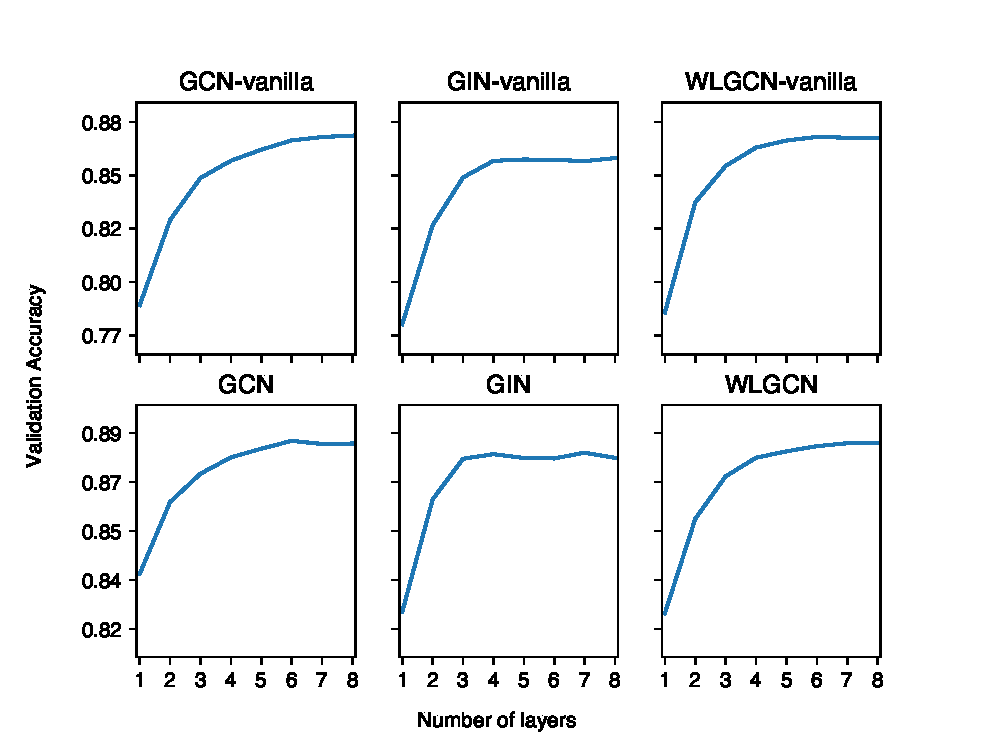
\includegraphics[width=.8\textwidth]{Figures/Chapter5/e1-layering}
    \caption{The effect of the number of \gls{dgn} layers to the performances of the models.}
    \label{fig:e1-layering}
\end{figure}

\subsection{Results on the E2 Experiments}\label{sec:e2-results}
For the second round of experiments, we fix the \gls{gcl} to the \gls{gcn} model with edge-handling capabilities, since it is the model that obtains the highest accuracy in \textbf{E1}.
The results of our experiments are reported in Table \ref{tab:e2-results}, where we average the computed metrics across the 5 test folds as usual.
\begin{table}[h!]
    \caption{Results of the 5-fold CV evaluation on various performance metrics. We report the global results (on the last row) as well as the results stratified by number of nodes per subgraph. For each stratification, we also report the related support (\ie the average number of graphs in the strata).}\label{tab:e2-results}
    \centering
    \footnotesize
    \renewcommand{\arraystretch}{1.2}
    \setlength{\tabcolsep}{0.7em}
    \begin{tabular}{lccccc}
      \toprule
      \Thead{Strata} & \Thead{Support} & \Thead{Accuracy} & \Thead{Sensitivity} & \Thead{Specificity} & \Thead{AUROC} \\
      \midrule
         1-10  & $243 (19)$ & $0.729 (0.020)$ & $0.851 (0.073)$ & $0.526 (0.113)$ & $0.820 (0.034)$\\
        11-20  & $711 (30)$ & $0.843 (0.006)$ & $0.919 (0.021)$ & $0.629 (0.050)$ & $0.892 (0.008)$\\
        21-30  & $526 (19)$ & $0.921 (0.008)$ & $0.969 (0.010)$ & $0.740 (0.052)$ & $0.954 (0.015)$\\
        31-40  & $967 (27)$ & $0.889 (0.012)$ & $0.937 (0.005)$ & $0.757 (0.040)$ & $0.950 (0.009)$\\
        41-50  & $1512 (21)$ & $0.928 (0.004)$ & $0.970 (0.008)$ & $0.635 (0.064)$ & $0.944 (0.011)$\\
        51-60  & $1679 (28)$ & $0.921 (0.004)$ & $0.971 (0.006)$ & $0.588 (0.038)$ & $0.950 (0.005)$\\
        61-70  & $1439 (23)$ & $0.947 (0.005)$ & $0.982 (0.006)$ & $0.644 (0.058)$ & $0.967 (0.005)$\\
        71-80  & $1159 (28)$ & $0.941 (0.006)$ & $0.980 (0.010)$ & $0.712 (0.087)$ & $0.972 (0.007)$\\
        81-90  & $372 (20)$ & $0.957 (0.008)$ & $0.998 (0.002)$ & $0.037 (0.075)$ & $0.925 (0.010)$\\
        91-100 & $378 (14)$ & $0.850 (0.017)$ & $0.964 (0.024)$ & $0.536 (0.061)$ & $0.888 (0.026)$\\
        \midrule
        \textbf{Overall} & $\mathbf{8985} (1)$ & $\mathbf{0.913} (0.003)$ & $\mathbf{0.965} (0.006)$ & $\mathbf{0.646} (0.042)$ & $\mathbf{0.948} (0.004)$\\
      \bottomrule
    \end{tabular}
\end{table}
In this case, we stratify the performances by number of nodes, in order to also analyze the model performances in relation to the size of the input subgraph. From the results, one can immediately see, by looking at the last row, how the model accurately predicts robustness better than all models tested in the \textbf{E1} phase by a large margin: this is probably caused by the largest size of the dataset, which usually results in major improvements with any \gls{ml} model, and in particular with \gls{dl} models. Specifically, we report an overall accuracy of $0.913 \pm 0.003$, as well as an AUROC of $0.948 \pm 0.004$. The model shows very high sensitivity ($0.965 \pm 0.006$) but a low specificity in comparison ($0.646 \pm 0.042$); this indicates that it is \quotes{harder} for the model to predict induced subgraphs that are not robust. This effect is a probable consequence of the class misproportion between negative and positive examples, which is around 86\% in favor of the positive class for this data sample. One result that is consistent across all measurements are the the very narrow standard deviations of the estimates, which indicate stable predictions regardless of the specific folds on which they are computed. To display this trend visually, we plot in Figure \ref{fig:e2-rolling-acc} the ROC curves obtained on the 5 test folds. Their similarity strongly indicates that the model performances are consistent across different test samples.
\begin{figure}
    \centering
    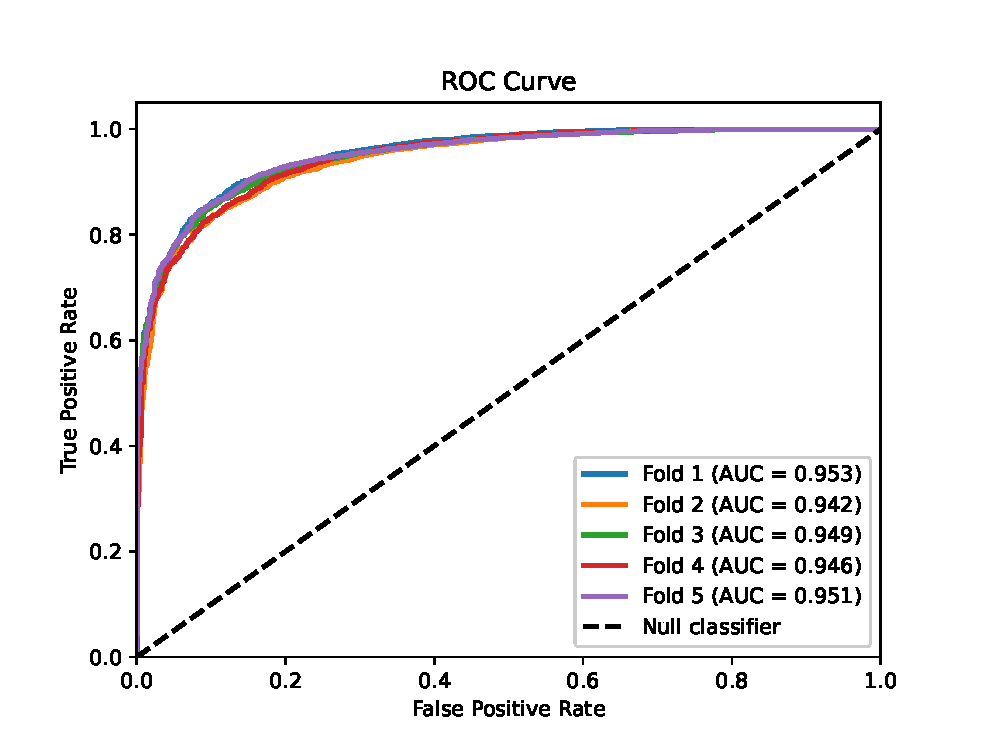
\includegraphics[width=.65\textwidth]{Figures/Chapter5/e2-roc-curve.eps}
    \caption{ROC curves for each of the five test folds. The black dashed line shows the performance of a baseline (\quotes{Null}) classifier that always predicts one class.}\label{fig:e2-roc-curve}
\end{figure}
The results of Table \ref{tab:e2-results} show a good performance of the model under the several stratifications tested. In particular, it performs better when dealing on subgraphs with 21-80 nodes, reaching an average in that strata AUROC of over 0.955. To better visualize this trend, we plot in Figure \ref{fig:e2-roc-curve} the rolling accuracy of the model, using a window size of 20, and averaging across the 5 test folds as usual. The plot clearly shows the improvement in accuracy as the number of nodes increases. Interestingly, when the size of the graph exceeds 80 nodes, the model performances start to decrease. This might be a consequence of the smaller sample sizes of subgraph with 81-100 nodes which occur in the dataset 3 times less on average than subgraphs with 21-80 nodes. The same trend can be noticed for smaller subgraphs, with up to 20 nodes. Finally, Figure \ref{fig:e2-conf-matrix} shows the confusion matrix of the predictions computed by the model, where the entries are the averages computed across the five test folds. In the plot, we can visualize the good performances of the model as regards the number of correctly predicted subgraphs (on the diagonal) with respect to the cases where the model makes wrong predictions. Looking at the anti-diagonal the confusion matrix, we can also see that the model has a higher rate of false positives than false negative. Again, this is expected behaviour due to class misproportion in the dataset.
\begin{figure}[h!]
    \begin{subfigure}[b]{0.48\linewidth}
    \centering
        \includegraphics[height=130px]{Figures/Chapter5/e2-rolling-acc.eps}
        \subcaption{}\label{fig:e2-rolling-acc}
    \end{subfigure}
    %
    \begin{subfigure}[b]{0.48\linewidth}
        \centering
        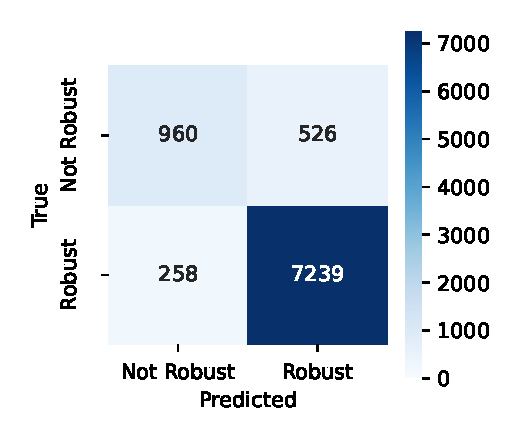
\includegraphics[height=130px]{Figures/Chapter5/e2-conf-matrix.eps}
        \subcaption{}\label{fig:e2-conf-matrix}
    \end{subfigure}
    \caption{({\scriptsize A}) Rolling mean accuracy (with a window of size 20), averaged over the 5 test folds, showing an increasing trend in performance as the number of graph nodes grows. ({\scriptsize B}) Confusion Matrix of the predictions computed by the model. Each entry of the matrix is the average of the corresponding entries in the five different confusion matrices of the test folds.}
\end{figure}

Lastly, we emphasize the fact that, once trained, the time needed to obtain a prediction from the model is in the order of milliseconds, while performing numerical simulations can be orders of magnitude slower. For this specific case, the simulation of most of the considered models (as detailed in Section \ref{sec:robustness-computation}) requires a amount of time in the order of minutes, while bigger models can take many hours to produce an output value. While training and evaluating the model is expensive, and can take hours, it needs to be performed only once. To conclude, we believe that, once perfected, methods inspired by our approach have the potential of enabling faster advances in understanding the functioning of cells through pathway modelling.

Following, we present two application cases of the model: the first is on the synthetic pathway shown in Figure \ref{fig:example-pathway}, and serves as an explanation tool of why the model performs sub-par in cases of smaller subgraphs; the second is an example of how the model can correctly infer the robustness relations in a real-world pathway.

\subsection{Application on Synthetic Data}
The lower prediction accuracy in the case of small graphs (1-10 nodes) can be put into perspective, in light of the fact the fact we trained the model with subgraphs in which kinetic, stoichiometric and initial concentration parameters have been omitted (as explained in Section \ref{sec:ppn}). In general, the smaller the graph, the higher the influence on its dynamics these parameters exert. As an example, let us consider the synthetic example of biochemical pathway introduced in Figure \ref{fig:example-pathway} and the corresponding pathway graph of Figure \ref{fig:pathway-graph}. Let us now consider the following kinetic and initial concentration (marking) parameters:
\begin{gather*}
  k1 = 1.0 \quad
  k3 = 0.01 \quad
  k5 = 0.01 \quad
  k7 = 0.3  \quad
  k2 = 5.0  \quad
  k4 = 0.1  \quad
  k6 = 5.0 \\
  m_0(A) = 50\quad
  m_0(B) = 50\quad
  m_0(C) = 100\quad
  m_0(D) = 100\\
  m_0(E) = 0\quad
  m_0(F) = 0\quad
  m_0(G) = 100\quad
  m_0(H) = 0.
\end{gather*}
We used these parameters to simulate the ODEs of Figure \ref{subfig:example-odes}, calculating the corresponding robustness by varying the initial concentration of each molecule in the interval $[-20\%,+20\%]$. The robustness values obtained with the simulations are displayed in Table \ref{tab:uc1-odes}. Analogously, in Table \ref{tab:uc1-predictions} we list the average and standard deviations obtained by the 5 different models evaluated in Section \ref{sec:e2-results} (one trained on the respective CV fold), when tasked to predict the robustness probabilities of some input/output pairs of interest.
\begin{table}[h!]
    % \scriptsize
    \centering
    \caption{({\scriptsize A}) Robustness values computed by numerical simulation of the ODEs in Figure \ref{fig:example-pathway}. Input molecules with initial concentration equal to 0 are omitted. Output molecules with identical robustness values are merged. ({\scriptsize B}) Probabilities of robustness obtained from the model for some relevant input/output combinations.}
    \begin{subtable}[b]{.59\linewidth}
      \centering
        \begin{tabular}{cccccc}
            \toprule
            \multirow{2}{*}{\textbf{Input}} & \multicolumn{5}{c}{\textbf{Output}}\\
             & \Thead{A} & \Thead{B} & \Thead{C/D} & \Thead{E/F} & \Thead{G/H}\\
            \midrule
              \textbf{A} & 1.00 & 0.73 & 0.99 & 1.00  & 1.00  \\
              \textbf{B} & 1.00 & 0.73 & 0.99 & 1.00  & 1.00  \\
              \textbf{C} & 1.00 & 1.00  & 0.00  & 0.99 & 0.99 \\
              \textbf{D} & 1.00 & 1.00  & 0.00  & 0.99 & 0.99 \\
              \textbf{G} & 1.00 & 1.00  & 1.00  & 1.00  & 0.50  \\
            \bottomrule
        \end{tabular}
        \caption{}\label{tab:uc1-odes}
    \end{subtable}%
    \begin{subtable}[b]{.39\linewidth}
        \centering
        \begin{tabular}{cc}
            \toprule
            \Thead{In/Out} & \Thead{Probability}\\
            \midrule
                $B/A$ & $0.3798 \pm 0.12$\\
                $A/F$ & $0.7254 \pm 0.18$\\
                $A/H$ & $0.8835 \pm 0.05$\\
                $C/F$ & $0.0793 \pm 0.11$\\
                $G/H$ & $0.2351 \pm 0.01$\\
            \bottomrule
        \end{tabular}
        \caption{}\label{tab:uc1-predictions}
    \end{subtable}
\end{table}
We remark that values in these two tables are not directly comparable: those in Table \ref{tab:uc1-odes} are exact robustness values, while those in Table \ref{tab:uc1-predictions} are probabilities of the robustness values to be greater than 0.5. In this specific case, the prediction turns out to be accurate in the case of input/output pairs corresponding to big induced subgraphs. This happens in the cases of the input/output pairs $A/F$ and $A/H$, whose induced subgraphs are among the largest ones. In contrast, the prediction is incorrect for $C/F$: in this case, the models predicts a small robustness probability, while the simulations give 0.99. We observe that the robustness value of this input/output combination is sensitive to the perturbation of parameters that have been discarded when constructing the dataset. In particular, if the initial (omitted) concentration of $C$ was $80$ instead of $100$, the robustness value of the pair $C/F$ would become $0.5$ rather than $0.99$. Another case when the model prediction is wrong is that of the pair The prediction turns out to be wrong also in the case of input $B/A$. In this case, the probability given by the network is under $0.50$, which contrasts to a value of $1$ obtained by the ODEs simulation. Even in this case, we notice that the parameters that have been omitted in the dataset might have a strong influence on the robustness, such as kinetic formulas and the multiplicity of the edge directed to node $B$. Finally, in the case of the pair $G/H$, the prediction gives a small probability of robustness and indeed the actual measured value is borderline ($0.50$). More in general, we observe that smaller subgraphs are less frequent than medium-sized subgraphs in the dataset. Thus, it is possible that the model has learned to be more accurate on the latter subgraphs (to maximize the accuracy), at the expense of making more errors when predicting the former.

\subsection{Application on a model of the EGF Pathway}
As a second use case, we consider the SBML model of the Epidermal Growth Factor (EGF) pathway proposed by Sivakumar et al. in \citep{sivakumar2011systems}. This model corresponds to model \texttt{BIOMD0000000394} of the BioModels database, and is shown in Figure \ref{fig:EGF} as represented by the CellDesigner tool \citep{funahashi2003celldesigners}. We adopt this visual representation style for this case study for readability, but the pathway can can be trivially translated into a \gls{ppn}.
\begin{figure}[t]
    \centering
    \includegraphics[width=12cm]{Figures/Chapter5/pathway394}
\caption{A model of the EGF pathway by Sivakumar et al. \citep{sivakumar2011systems}.Image generated form the SMBL file in the BioModels database using the CellDesigner tool.}\label{fig:EGF}
\end{figure}
The pathway describes, in a simplified way, the transduction of the EGF signal, and the consequent activation of the mitogenesis and cell differentiation processes (modelled as an abstract species in the pathway). When the EGF signal protein is available in the cell environment, it can be perceived by the receptor protein EGFR (where R stands for Receptor), which then initiates a cascade of reactions inside the cell, ultimately leading to the activation of mitogenesis and differentiation. The initial steps of the pathway give rise to a rather big complex, involving an activated EGFR dimer and a number of other proteins (the big box in the upper-left corner of Figure \ref{fig:EGF}). The formation of such complex is described in a very simplified way in this pathway model, by concentrating everything in only two reactions. The big complex then promotes a cascade of reactions inside the cell, which are modelled more in detail.

Considering the mitogenesis and differentiation (abstract) species as output (in pink, bottom left corner of Figure \ref{fig:EGF}), with respect to EGF and EGFR as input (in green and yellow, respectively, top left corner of Figure \ref{fig:EGF}), numerical simulations assign a very high robustness ($>0.995$) in both cases. This is actually expected in a signal transduction pathway, since it behaves as an amplifier that must be able to activate the target cell process despite of perturbations in the signal and receptor concentrations. On the other hand, if we look at the robustness of the first portion of the pathway up to the creation of the big complex, we can then observe a different behavior. Specifically, if we consider the big complex as output and EGF as input, we still obtain a very high robustness ($>0.999$). However, when the input is EGFR, we obtain a robustness value of only $0.19$. Again, this is not surprising, since EGF is modelled in the pathway as a promoter of the first reaction (\ie, it is not consumed), while EGFR is a reactant and it will be included in the big complex.

In this case, the model correctly captures the different roles of EGF and EGFR. Indeed, using EGF as input and the big complex as output, the model gives $0.9474 \pm 0.014$ as probability of robustness, whereas it gives $0.145 \pm 0.121$ when the input is with EGFR. The model captured also captures the robustness of the whole model, namely the previous case where either EGF or EGFR were considered as input, and the abstract mitogenesis and differentiation as output. Precisely, it gives probability $0.973 \pm 0.005$ with EGF as input and $0.970 \pm 0.008$ with EGFR as input.

\section{Conclusion and Further Work}
This work shows experimentally, and for the first time, that we can correlate structural properties of biological pathways to their dynamical properties. We consider this result very promising and deserving of further investigation. Indeed, the promise of this approach if that of creating a novel class of learning methods for pathways, which could help to better study the functioning of living cells.

We consider this approach impacting for two main reasons. Firstly, predicting dynamical properties of pathways with Deep Learning methods is faster than performing numerical or stochastic simulations. While the training process is expensive in terms of time required, it needs to be performed only once, and can be amortized nicely as more and larger subgraphs are used. Secondly, our approach works considering only a minimal amount of information regarding the pathway: its structure, an input and output node, and the types of nodes and relations between them. Hence, it is applicable even in cases where other information, such as kinetic constants, is not available.

One research direction to pursue in the immediate future concerns evaluating this architecture on datasets where the information we omitted in the present study has been added. For example, it would be interesting to assess how the addition of edge labels (multiplicities of reactants/products), or kinetic formulas, would affect performances. These additional information could be useful, for example, to help the preditions of the model in case of smaller subgraphs. Moreover, one could think to extend this approach to the assessment of other related dynamical properties of pathways, such as other notions of robustness, or even completely different ones such as monotonicity, or oscillatory and bistability properties.

We also believe this work opens up fascinating research scenarios to pursue in the medium term. One important aspect that needs further investigation is model explainability. Even though their predictive result are very often excellent, neural networks are sometimes seen as black-box since the exact function (in this case, from pathway structure to robustness) they approximate is difficult to characterize. One possible research direction is to investigate generative models, to uncover the underlying structure of pathway space and help design better predictive models, as well as provide better explanations to the decisions they take.

\part{Deep Generative Learning on Graphs and Applications to Computational Chemistry}\label{part:generative}
\chapter{Deep Generative Learning on Graphs} % Main chapter title
\label{ch:deep-generative-learning-graphs}
In this chapter, we discuss the graph generation problem. The term \quotes{graph generation} is purposedly kept broad, to include a variety of methodologies which learn processes that generate graphs from a set of training examples. This research field originates from generative models of graphs for the theoretical understanding of graph properties, which have been studied thoroughly since the '50s in the field of graph theory. The first known generative model is the  Erd\"{o}s-R\'{e}nyi (ER) model \cite{erdos1959randomgraphs}. The ER model studies random graphs, where the connectivity among graph nodes is modeled independently. This model is useful to study theoretical properties of graphs, such as how the global connectivity of the graph evolves as its size grows. Another historical model of graphs is the  Watts-Strogatz (WS)  model \cite{watts1998smallworld}. The WS model concerns \quotes{small world} graphs, \ie graphs where it is possible to reach any other node in the graph with very short paths, regardless of their ize. This property arises in several real-world graphs such as social and electrical networks. Lastly, the Barab{\'a}si-Albert (BA) model \cite{barabasi1999prefatt}, which models the so-called \quotes{preferential attachment} property, where the connectivity potential of a node is directly proportional to its number of neighbors. While being useful to the study and understanding of graph properties, these models usually fail to generalize to real-world graph distributions, because they can only model one or a limited number of graph properties, and that their parameters cannot be learned from data in general. Other methods such as stochastic block models \citep{airoldi2008mixedstochasticblock}, exponential random graphs \citep{robins2007exponentialrandomgraphs}, and Kronecker graphs \citep{leskovec2010kronecker} can approximate more complex graph distributions such as graphs with communities, but are still limited to specific kinds of graphs and scale poorly to large datasets.
These limitations clearly highlight that, in order to generate graphs for practical applications, a more powerful class of learning models is needed. In this chapter, we review a variety of generative models of graphs based on Deep Learning approaches. The advantages of such models are the possibility to approximate complex distributions efficiently and effectively, and the flexibility to use different generative paradigms to adapt to the task at hand.

\section{The Challenges of Graph Generation}
The problem of generating graph structures from arbitrary distributions is arguably harder than their predictive modeling. Some of the challenges that need to be addressed when designing deep generative models of graphs are related to the complexity of graph spaces. In particular, we report the following:
\begin{itemize}
    \item \emph{size of graphs spaces}. Graphs spaces are combinatorial, and thus very large. For example, the size of the space of undirected graphs with $m$ nodes is ${m \choose 2} = \frac{m(m-1)}{2}$, which becomes very large even for graphs with a moderate number of nodes. Thus, trivial approaches such as exhaustive enumeration are generally intractable. Moreover, real-world graph distributions are usually defined over attributed graphs with variable size, which makes the search space even larger;
    \item \emph{discreteness of graphs spaces}. Graphs are discrete objects. This contrasts with the nature of neural networks, which can backpropagate only through continuous and differentiable objects. Hence, the learning process must be accomodated to work with discrete structures;
    \item \emph{sparsity of graphs spaces}. For most generative tasks, only very small subsets of graph space contain graphs with non-zero probability. Thus, any generative method should be designed to focus on regions where interesting graphs are contained, to avoid efficiency issues;
    \item \emph{complex dependencies}. Most real-world graph have hard structural constraints that are very difficult to enforce on a generative model (which is inherently stochastic). For example, cycle graphs are such that if only one edge is missplaced, the graph is not a cycle anymore;
    \item \emph{non-unique representations}. In general, graphs are invariant under node permutation. Thus, the same graph can be potentially represented by up to $n!$ possible adjacency matrices, depending on the node permutation. This poses constraints on the kind of graph representations a generative model can learn. For example, generative methods that map graphs into a latent space must take into account that different node permutations of the same graph must map to the same latent vector. While invariance to node permutation can be addressed by assuming an order of the graph nodes, this introduces the necessity to maintain order consistency among different graphs.
\end{itemize}

\section{Generative Tasks}
The family of \glspl{dgm} of graphs is flexible enough to model different kinds of generative tasks. Loosely following the taxonomy proposed by \citet{guo2020systematicreviewgenerativegraphs}, we distinguish two main tasks related to graph generation:
\begin{itemize}
    \item \emph{unconditional generation}, where the task is to explicitly learn a distribution $p(\Graph{g})$ over graphs, or some parametrized function that produces samples from it. Here, the term \quotes{unconditional} refers to the fact that the generation starts with drawing a vector $\Vector{z} \in \Real^z$ from some easy to sample prior distribution $p(\Vector{z})$, which is usually assumed to be an isotropic Gaussian or a uniform distribution;
    \item \emph{conditional generation}, where the aim is to learn a conditional distribution $p(\Graph{g} \given \Vector{y})$ with $\Vector{y} \in \Real^y$, or the corresponding parameterized sampling mechanism. The purpose of the conditioning vector is to drive the generative process towards producing a graph with desired characteristics. For example, one might want to generate a graph whose structure resembles that of a graph given as input to the \gls{dgm}. In this case, $\Vector{y}$ is the representation of the conditioning graph.
\end{itemize}
Hereafter, we consider the task of unconditional generation, where we assume access to a dataset of graphs $\Data = \Set{\Graph{g}_i}_{i=1}^n$. Notice from the notation that, at least for the moment, we focus on unattributed graphs. Broadly speaking, defining a \gls{dgm} of graphs requires to specify two components: a \emph{graph decoder}, which takes care of generating a graph, and an end-to-end generative framework used to optimize the model parameters. As regards the latter, common generative frameworks include \glspl{vae}, \glspl{gan}, and flow-based models \citep{rezende2015normalizingflows}. Here, we only describe approaches based on the first two.

\section{Graph Decoders}
The graph decoder is the architectural component that outputs some conditional distribution, which can be sampled to generate a graph. If the framwork in which the decoder is placed allows for inference (such as the \gls{vae}), the conditional is also learned with maximum likelihood; otherwise, (such as with \glspl{gan}) it is used only for sampling, and its parameters are optimized with adversarial training. Ideally, graph decoders should generate permutation invariant graphs; however, this is rarely the case. The major hurdle to devise permutation invariant graph decoders is their computational cost; even though some methods do exist \citep{ermon2020permutationinvariantgraphgeneration}, they are still too inefficient to be deployed in real world scenarios. Thus, in the following, we assume non-invariance.
One particular caveat that needs to be addressed during the training phase of a graph decoder is maintaining the differentiability of the architecture while still generating hard graph samples. This is critical especially in \gls{gan}-like architectures, where the discriminator must be trained with actual graphs. As with sequence generation with \glspl{rnn}, the same techniques (straight-trough gradient estimation, reparameterization, or even reinforcement learning-based techniques \cite{williams1992reinforce}) can be used for this purpose. There are two main paradigms to implement adaptive graph decoders, which we detail in the following.

\subsubsection*{One-shot Decoders}
This class of graph decoders outputs a dense probabilistic adjacency matrix $\ProbAdjMatrix{g} \in \Real^{n \times n}$, where $n$ is the maximum number of nodes allowed. The probabilistic matrix is sampled entry by entry to produce an actual adjacency matrix. The entries of the matrix are modeled as independent Bernoulli variables, which indicate the presence or absence of an edge. In some cases, the elements in the adjacency matrix $a_{ii}$ are modeled as independent Bernoulli variables that specify if a node belongs to the graph or not. In practice, the entries of the matrix are produced by a neural network with sigmoid outputs that predicts an $n \times n$ vector. Thus, the adjacency matrix can be sampled in parallel (hence the term \quotes{one-shot}). Two possible approaches to specify a one-shot decoder are:

\begin{itemize}
    \item \emph{graph-based} decoders, which require a graph representation $\Vector{z}$. In this case, the decoder models the conditional as follows:
    $$p(\ProbAdjMatrix{g} \given \Vector{z}) \approx \prod_{i=1}^n \prod_{j=1}^n p_{\Param}(a_{ij} \given \Vector{z}),$$
    where $p_{\Param}$ is a neural network that predicts the matrix from the graph representation;
    \item \emph{node-based} decoders, which require a matrix of node representations $\Matrix{Z} \in \Real^{n \times z}$. In this case, the decoder models the conditional as follows:
    $$p(\ProbAdjMatrix{g} \given \Matrix{z}) \approx \prod_{i=1}^n \prod_{j=1}^n p_{\Param}(a_{ij} \given \Vector{z}_i, \Vector{z}_j),$$
    where $i$ and $j$ range over the matrix rows. In this case, $p_{\Param}$ is a neural network that takes as input pair of node representations, and applies a sigmoid function to their dot product. The idea is that nodes that are close in representation space should be more likely to be connected.
\end{itemize}
One-shot approaches are usually fast to train and to take samples from. However, they are too simplistic, in that they assume the edges are generated independently (which is usually not the case for real-world graphs). Furthermore, the maximum number of nodes must be pre-specified, which makes them unable to generalize to larger graphs.

\subsubsection*{Autoregressive Decoders}
Autoregressive decoders assume that graphs are generated by some sequential process that involves its set of nodes. Specifically, the generative process is the following:
$$p(\Graph{s}) = \int p(\Graph{s}, \pi)\, d\pi = \int p(\Graph{s} \given \pi)\, q(\pi)\, d\pi,$$
where $\Graph{s}$ are sequences that generate graphs one component at a time, and the order of generation is given directly or indirectly by a nodes permutation drawn from a prior $q(\pi)$. The idea is to decompose the generating sequence autoregressively as follows:
$$p(\Graph{s}) = \int p(\Graph{s}_i \given \Graph{s}_{[<i]}, \pi)\, q(\pi)\, d\pi.$$
However, this requires to integrate over all $n!$ possible node permutations, which becomes intractable for moderately large graphs. An approximate solution to this issue is to assume some ordering and create the sequences before training, as a preprocessing step. Once the sequence are fixed, the chain-rule decomposition becomes tractable:
$$p(\Graph{s}) \approx p_{\Param}^{\pi}(\Graph{s}) = p_{\Param}^{\pi}(\Graph{s}_i \given \Graph{s}_{[<i]}).$$
Depending on the nature of the graph generating sequence, we distinguish four possible approaches to develop autoregressive graph decoders:
\begin{itemize}
    \item \emph{node-based} approaches decompose the graph as a sequence of actions performed on an initially empty graph. These action correspond to decisions such as whether to add a node to the existing graph, and which nodes it must be connected to. In this case, $\Graph{s}_{[<i]}$ is a vector that represents the current state of the graph. For all these models, one has two options as to how to implement the autoregressive network. One approach is to use a hierarchy of \glspl{rnn}: one keeps track of the state of the nodes added to the graph, and the other is responsible to connect newly added nodes to the current graph, given the state of the first \citep{you2018graphrnn}. The other choice is to update the state of the current graph with a \gls{dgn}, which is passed to the networks responsible of deciding which action to perform \citep{li2018learningdeepgmg};
    \item \emph{edge-based} approaches decompose the graph as a sequence of edges. To produce an ordered sequence of edges, one must first order its nodes, then label the nodes with progressive integers, and then sort its set of edges in lexicographic order. In this case, $\Graph{s}_{[<i]}$ represents the state of the graph indirectly, by keeping memory of the edges of the sequence already generated. These approaches are mostly implemented with \glspl{rnn} \citep{goyal2020graphgen,bacciu2019edgegraphgenrnn};
    \item \emph{rule-based} approaches can be applied in cases where the graph generation can be decomposed in a sequence of production rules over some known grammar (\eg molecules or computer programs) \citep{kusner2017grammarvae,dai2018sdvae}. In this case, the model generates a sequence of production rules to construct a desired graph;
    \item \emph{motif-based} approaches decompose the graph as a sequence (or even a tree) of \emph{motifs}, \ie very small and manageable subgraphs, which are combined together adaptively. Here, the challenge is mainly how to decompose the graphs into sequences of motifs,
\end{itemize}
A special kind of sequential decomposition for graphs is one applied to molecules. In fact, molecular graphs can be linearized with approximated graph canonization into strings of the so-called \gls{smiles} language \citep{weininger1988smiles}. In practice, the SMILES encoding consists in transforming a molecular graph in a \gls{dpag}, breaking cycles in a certain order. Than, the \gls{dpag} is traversed in depth-first order, and a character is associated in an orderly manner to the atoms, chemical bonds and other chemical constructs. The result is a string representing the graph structure. Various canonization techniques can be applied during the process, such that the obtained string is unique for each unique graph (up to a few degenerate cases).

When a domain-specific linearization techniques such as SMILES are not available, the sequences representing the graph generative process are constructed based on some node ordering strategy. One general strategy to do so is to choose one node at random, then visit the graph nodes with a depth-first or breadth-first traversal. The order by which the nodes are visited is used to determine the order of the elements in the sequences. Clearly, this approach is not optimal since it heavily depends on the starting node, and may produce very different sequences for different starting node choices. However, it has been shown to work empirically \citep{you2018graphrnn,li2018learningdeepgmg,bacciu2019edgegraphgenrnn,goyal2020graphgen}. The pros and cons of autoregressive decoders are orthogonal to those of one-shot decoders: briefly, they allow to generate variable-sized graphs seamlessly, and they can model dependencies between nodes and edges by means of the autoregressive property. However, both training and sampling processes are slower in terms of computational time, because the graphs are reconstructed one sequence element at a time and not in parallel.

\section{Performance Evaluation}\label{sec:evaluation-generative-graphs}
The desired end result of training a generative model is that the structure of samples generated by the network should resemble that of graphs in the training set, without being identical. This is a very different setting with respect to predictive tasks, since the samples of a generative model do not exist until they are generated. Hence, one does not have access to held-out ground truth values to measure generalization. Furthermore, the model can very easily obtain deceptive-looking performances by learning to replicate training graphs exactly, or repeating the same graph typology over and over. Thus, one critical aspect of using generative models of graphs is how to assess performances. Below, we define two broad classes of metrics that allow the evaluation of graph models, assuming the availability of a training sample $\TrainingSample \subseteq \Data = \Set{\Graph{g}}_{i=1}^n$ , and a collection\footnote{Here, we use the term \quotes{collection} to indicate a multiset, meaning that it can possibly contain duplicate elements.} $\GeneratedSample = \Set{\Graph{g'}}_{i=1}^m$ of samples generated by the model.

\subsection{Quantitative Metrics}
\emph{Quantitative} metrics measure the rate at which the generative model produces diverse and heterogeneous graphs, without taking into account structural similarity. The three main quantitative matrics considered in the literature are:
\begin{itemize}
    \item \emph{novelty} measures the ratio of generated samples that are not training samples. A high novelty indicates that the model has not learned to replicate training graphs. Formally, it is measured as $1 - \frac{|\GeneratedSample \Inter \TrainingSample|}{|\TrainingSample|}$;
    \item \emph{uniqueness} measures the ratio of unique graphs with respect to the total number of graphs generated. A low uniqueness rate might indicate that the model has overfit one specific typology of graph. To calculate uniqueness, one first checks every graph for isomorphism with every other graph in the generated sample, removing them. If the resulting set of unique graphs is indicated by $\UniqueSample$, uniqueness can be simply calculated as $\frac{|\UniqueSample|}{|\GeneratedSample|}$.
    \item \emph{validity} measures the ratio of generated graphs that respect some validity constraint, out of the total number of graphs generated. To calculate validity, one needs to check wheter every generated graph satisfies some structural constraint or not (\eg the presence of a cycle). If $\ValidSample$ is the collection of graphs that satisfy the structural constraints, validity is calculated as $\frac{|\ValidSample|}{|\GeneratedSample|}$. This metric is particularly useful in molecular generation tasks, since chemically invalid molecules are useless. When assessing validity is required, novelty and uniqueness are usually conditioned on validity first, meaning that the all the invalid graphs are removed from $\GeneratedSample$ before calculating these two metrics.
\end{itemize}

\subsection{Qualitative Metrics}
Quantitative metrics give only one side of the spectrum relatively to how a generative model is performing. For example, assessing novelty alone might be misleading, since a high novelty rate can also be associated to underfitting (meaning that the model generates graphs very different from the training sample, which are trivially novel). Thus, a proper evaluation of generative models must also include a series of metrics that consider the structural properties of the generated graphs. We call such metrics \emph{qualitative}. The framework under which qualitative metrics are assessed consists of comparing the empirical distribution of a certain graph property in the training sample, to the empirical distribution on the generated sample. Given a generic graph with $d$ nodes, coming from one of the two samples indifferently, a relevant subset of such properties includes:
\begin{itemize}
    \item node degree distribution, that is, an $d$-dimensional vector where each position contains the degree of the corresponding node. Notice the the length of the vector may differ across different graphs, since their number of nodes may change;
    \item clustering coefficient distribution. The clustering coefficient of a node $v$ is defined as the ratio between the number of actual connections between neighbors of $v$ out of the total number of possible connections. In other words, it is a relative measure of how many \quotes{closed triangles} (fully connected graphs with three nodes) the node is part of. Similarly to the node degree distribution, it consists of an $d$-dimensional vector where each position contains the clustering coefficient of the corresponding node;
    \item number of nodes of the graph, which is a single integer;
    \item number of edges of the graph, which is again a single integer;
    \item average orbit counts. Orbits are subgraph with 4 nodes. Counting orbits in a graph can be viewed as a generalization of the clustering coefficient to 4-node subgraphs instead of triangles. In practice, it consists in a $dk$-dimensional vector, where $k$ is the number of orbits considered;
    \item \gls{nspdk} \citep{costa2010nspdk}, which measures the similarity between two graphs by counting the number of matching induced subgraphs between them. The subgraphs are derived node-wise, by considering neighborhoods of a node comprising nodes at increasing path lengths. Differently from the other qualitative metrics, the \gls{nspdk} provides a global measure of similarity between graphs, since it is based on multiple subgraph matchings. In practice, it is a vector of length $m-1$ ($n-1$, respectively), where each position measures the similarity of the graph with another graph in the sample.
\end{itemize}
Once the graph properties are calculated for each graph in the sample, there are two options to measure the distance between the empirical distribution of the training sample versus the generated sample, based on their respective number of elements:
\begin{itemize}
    \item if $n = m$, one can compute their empirical \gls{kld} as follows:
    $$\EKLD{\Prop(\GeneratedSample)}{\Prop(\TrainingSample)} = \frac{1}{n} \sum_{i=1}^{n} \Prop(\Graph{g}_{(i)}) \log \Par{\frac{\Prop(\Graph{g'}_{(i)})}{\Prop(\Graph{g}_{(i)})}},$$
    where $\Prop$ is one of the properties mentioned above;
    \item if $n \neq m$, one can either concatenate all the values of the property for each each in the sample, and then fit a histogram with an equal number of bins to make their length match in order to apply the empirical \gls{kld}. Another, more general, approach to compare distribution when the two samples have different lengths is to compute their \gls{mmd} \citep{gretton2012mmdkernel}. Intuitively, the \gls{mmd} measures the distance between two distributions as the sum of the distances of between their matching moments. The computation of these distances can be generalized to an infinite space of moments by applying a kernel trick \citep{smola2008kernels}.
\end{itemize}

\section{A Model for Edge-Based Graph Generation}
\subsection{Introduction}
In this section, we present an original contribution. Specifically, we introduce a novel generative model for graphs, capable of generating unattributed graphs coming from very different graph distributions. We transform graphs into sequences of ordered edges, from which we extract two sequences derived from the edge endpoints. We use a model composed of two \glspl{rnn} to learn the probability distribution of such sequences: the first is an autoregressive network which generates a specification of the graph to produce, which is completed into a graph by the second network. We experiment extensively with the proposed model, comparing its performances with a pool of baselines, one of which is a \gls{dgm} of graphs that holds state-of-the-art performances at the generative task. The experimental framework has been designed to evaluate the proposed model on concerning both quantitative and qualitative aspects, as discussed in Section \ref{sec:evaluation-generative-graphs}. Our experiments demonstrate that, under our evaluation framework, the proposed model is able to perform at, and sometimes surpass, the state-of-the-art in the task of generating graphs coming from very different distributions. Furthermore, we study the effect of changing the order of the edge sequence by experimenting with different node orderings. We show that the chosen node ordering strategy  is more effective for learning complex dependencies than the alternatives, and produces graphs of better quality.

\subsection{Methods}
In this section, we present the methodologies used to develop the model. In particular, we formally introduce the concept of ordered edge sequences, we develop the model,and  we show how it is trained and how graph generation is achieved.

\subsubsection*{Ordered Edge Sequences}
Let $\Graph{g} = \Tuple{\Nodes{g}, \Edges{g}}$ be a fully connected unattributed graph with $n$ nodes and $m$ edges. We assume $\Graph{g}$ is undirected for simplicity, without loss of generality. Let $\gamma: \Nodes{g} \shortrightarrow \Natural_{+}$ be a bijective node labelling function which assigns a unique positive integer (which we call node ID) to each node in the graph; thus, $\gamma$ defines a total order over the nodes of $\Graph{g}$. The \emph{ordered edge sequence} $\Cal{S}$ of graph $\Graph{g}$ is the sequence of pairs:
$$\OES{S}_{\Graph{g}} = ((s_1, e_1), (s_2, e_2), \ldots, (s_m, e_m)),$$
where $(\gamma^{-1}(s_i), \gamma^{-1}(e_i)) \in \Edges{g}$, and such that it is ordered lexicographically according to the IDs assigned to the nodes, \ie $(s_i,e_i) \leq (s_j,e_j)$ if and only if $s_i < s_j$, or $s_i = s_j$ and $e_i \leq e_j$. Given a generic pair $(s_i,e_i) \in \OES{S}_{\Graph{g}}$, we call $s_i \in \Natural_{+}$ its \emph{starting node} and $e_i \in \Natural_{+}$ its \emph{ending node}. Finally, let us define the \emph{starting sequence} $\Start{\OES{S}_{\Graph{g}}} = (s_1, s_2, \ldots, s_m)$, the sequence corresponding of starting nodes ordered as in $\Graph{e}$, and analogously, the \emph{ending sequence} $\End{\OES{S}_{\Graph{g}}} = (e_1, e_2, \ldots, e_m)$, corresponding to the ending nodes ordered as in $\OES{S}$. For conciseness, let us omit the dependece of $\OES{S}_{\Graph{g}}$ on the graph $\Graph{g}$, and of the starting and ending sequences from $\OES{S}_{\Graph{g}}$ whenever they are clear from the context. Clearly, the choice of the labelling function $\gamma$ is critical in determining the ordered sequence of a graph. Given the graph $\Graph{g}$, we choose to implement $\gamma$ with the following algorithm:
\begin{itemize}
    \item first, select a node $v_1$ at random from its set of nodes $\Nodes{g}$, and set its node ID as $\gamma(v_1) = \SF{1}$;
    \item then, traverse the graph in breadth-first order. Let $V = (v_2, v_3, \ldots, v_{n})$ be the ordered sequence of nodes visited during the traversal, excluding $v_s$. Assign node ID $\gamma(v_i) = \SF{i},\, \forall v_i \in V,\, i=2, \ldots, n$.
\end{itemize}
Assuming graph $\Graph{g}$ has the structure shown in Figure \ref{fig:example-graph}, and that node $v_1$ is chosen as the root node for the visit, an example of how the graph nodes are labelled by $\gamma$ is shown in Figure \ref{fig:labelled-graph}. Notice that $\gamma$ is trivially bijective, since it assigns a different integer to each node. Once the nodes are labelled, the ordered edge sequence of $\Graph{g}$ is $\OES{S} = (\OElem{1}{2},\OElem{1}{3},\OElem{1}{4},\OElem{3}{4},\OElem{3}{5})$, with $\tau_S = (\SF{1},\SF{1},\SF{1},\SF{3},\SF{3})$ and $\tau_E = (\SF{2},\SF{3},\SF{4},\SF{4},\SF{5})$. Notice that the graph can be readily reconstructed from its orderd edge sequence by first applying the inverse function $\gamma^{-1}$ to each element of its pairs to obtain $\Edges{g}$, which in turn gives $\Nodes{g}$ since we assumed that $\Graph{g}$ is fully connected.

\begin{figure*}[h!]
    \begin{subfigure}[b]{0.48\linewidth}
        \centering
        \resizebox{.8\textwidth}{!}{

\tikzset{every picture/.style={line width=0.75pt}} %set default line width to 0.75pt

\begin{tikzpicture}[x=0.75pt,y=0.75pt,yscale=-1,xscale=1]
%uncomment if require: \path (0,169); %set diagram left start at 0, and has height of 169


% Text Node
\draw  [line width=2.25]   (45, 32) circle [x radius= 14.21, y radius= 14.21]   ;
\draw (45,32) node   [align=left] {\begin{minipage}[lt]{13.600000000000001pt}\setlength\topsep{0pt}
\begin{center}
$\displaystyle v_{1}$
\end{center}

\end{minipage}};
% Text Node
\draw    (115, 42) circle [x radius= 14.21, y radius= 14.21]   ;
\draw (115,42) node   [align=left] {\begin{minipage}[lt]{13.600000000000001pt}\setlength\topsep{0pt}
\begin{center}
$ $
\end{center}

\end{minipage}};
% Text Node
\draw    (35, 92) circle [x radius= 14.21, y radius= 14.21]   ;
\draw (35,92) node   [align=left] {\begin{minipage}[lt]{13.600000000000001pt}\setlength\topsep{0pt}
\begin{center}
$ $
\end{center}

\end{minipage}};
% Text Node
\draw    (105, 132) circle [x radius= 14.21, y radius= 14.21]   ;
\draw (105,132) node   [align=left] {\begin{minipage}[lt]{13.600000000000001pt}\setlength\topsep{0pt}
\begin{center}
\end{center}

\end{minipage}};
% Text Node
\draw    (165, 102) circle [x radius= 14.21, y radius= 14.21]   ;
\draw (165,102) node   [align=left] {\begin{minipage}[lt]{13.600000000000001pt}\setlength\topsep{0pt}
\begin{center}
$ $
\end{center}

\end{minipage}};
% Connection
\draw    (42.66,46.02) -- (37.34,77.98) ;
% Connection
\draw    (59.07,34.01) -- (100.93,39.99) ;
% Connection
\draw    (52.31,44.19) -- (97.69,119.81) ;
% Connection
\draw    (113.43,56.13) -- (106.57,117.87) ;
% Connection
\draw    (117.71,125.64) -- (152.29,108.36) ;

\end{tikzpicture}}
        \caption{}
        \label{fig:example-graph}
    \end{subfigure}
    \begin{subfigure}[b]{0.48\linewidth}
        \centering
        \resizebox{.8\textwidth}{!}{\input{Figures/Chapter6/labelled-graph.tex}}
        \caption{}
        \label{fig:labelled-graph}
    \end{subfigure}
    \caption{({\scriptsize A}): an example graph, where the starting node $v_1$ of the labelling algorithm is marked with a thicker border. ({\scriptsize B}): the same graph, where nodes are labelled according to a breadth-first visit of the graph rooted at $v_1$.}
    \label{fig:labelling-example}
\end{figure*}

\subsubsection*{Model}
Our goal is to model $p(\OES{S})$, the probability of ordered edge sequences, using a dataset $\Data = \Set{\OES{S}_{(i)}}_{i=1}^n$. Our key observation is that any ordered edge sequence $\OES{S}$ is uniquely defined by its starting and ending sequences. Therefore, instead of working on the ordered edge sequence directly, we work on their starting and ending sequences. Specifically, we model the probability of sampling $\OES{S}$ from $p(\OES{S})$ as follows:
$$p(\OES{S}) = p(\tau_S, \tau_E) = p(\tau_E \given \tau_S)\, q(\tau_S) = \prod_{i=1}^{|\OES{S}|} p(e_i \given s_i)\, \prod_{j=1}^{|\OES{S}|} q(s_j \given s_{[<j]}).$$
Intuitively, the generative process specified by the distribution is the following:
\begin{itemize}
    \item first, one samples $\tau_S$ from a prior probability $q(\tau_S)$, which is modeled autoregressively;
    \item once $\tau_S$ is available, it is used to condition the prediction of the ending sequence $\tau_E$.
\end{itemize}
Once both $\tau_S$ and $\tau_E$ are available, the ordered edge sequence (and thus, the corresponding graph) an be reconstructed simply pairing their elements. Here, we make an important remark. Notice that the the probability of $q(\tau_S)$ is modeled autoregressively, while the conditional $p(\tau_E \given \tau_S)$ is not. This means that to generate a sequence, the only stochastic part in the model relates to $q(\tau_S)$, while predicting $\tau_E$ is deterministic once $\tau_S$ is known. One possible interpretation of $q(\tau_S)$ is that it acts as a \quotes{soft prior} of the structure of the graph: in fact, it specifies a subset of relevant nodes for the generation and their degree, expressed as the number of times they appear in the starting sequence. The conditional $p(\tau_E \given \tau_S)$ uses this information to \quotes{complete} the graph based on the information provided by the prior.

\subsubsection*{Training}
The model specified above is implemented as two \glspl{rnn} in cascade, which we refer to as $q_{\EncParam}$ and $p_{\DecParam}$ respectively. The two sequences (starting and ending) are first encoded as sequences of $(k+2)$-dimensional one-hot vectors, where $k$ is the largest node ID assigned by $\gamma$ to any node in the dataset, and $+2$ is added for the start of sequence and end of sequence tokens. We indicate the one-hot encoded starting sequence with the notation $\Vector{s} = (\Elem{s}{1}, \ldots, \Elem{s}{|\tau_S|}, \EOS)$, where $\Elem{s}{i} \in \Real^{k+2}$, and analogously, we use $\Vector{e} = (\Elem{e}{1}, \ldots, \Elem{e}{|\tau_E|})$ for the one-hot encoded ending sequence, with $\Vector{e}_i \in \Real^{k+2}$. Notice that an end of sequence token is added to $\Vector{s}$: when it is predicted, the autoregressive process that yields $\Vector{s}$ is interrupted. Our dataset is has thus the following form: $\Data = \Set{(\Vector{s}_{(i)}, \Vector{e}_{(i)})}_{i=1}^n$. Focusing on a single training pair $(\Vector{s}, \Vector{e})$, we explain the feed-forward phase of the network. Firstly, the sequence $\Vector{s}$ is processed by $q_{\EncParam}$. Given an element $\Elem{s}{i} \in \Vector{s}$, the per-element output of $q_{\EncParam}$ is obtained as follows:
\begin{align*}
    \Elem{h}{i} &= \Op{GRU}_{\EncParam}(\Elem{h}{i-1}, \Matrix{E}^{\Transpose}\Elem{s}{i-1})\\
    \Elem{o}{i} &= \softmax(\Matrix{V}_{\EncParam}\Elem{h}{i} + \Vector{b}).
\end{align*}
In the formula above, $\Matrix{E} \in \Real^{k \times h}$ is an \emph{embedding matrix} whose entries are learnable, and the dot product selects the column of $\Vector{E}$ corresponding to the embedding of the node ID assigned to $\Elem{s}{i}$. Furthermore, $\Elem{h}{i} \in \Real^h$ is a hidden state, $\Op{GRU}_{\EncParam}$ is a multi-layer GRU network, $\Matrix{V}_{\EncParam} \in \Real^{h \times (k+2)}$ is an output weight matrix,  $\Vector{b} \in \Real^{k+2}$ is a bias vector, and $\Elem{o}{i}$ is an output distribution over all the possible node IDs. The process is initialized by setting $\Elem{s}{0} = \SOS$ and $\Elem{h}{0} = \Zeros$. We use teacher forcing, meaning that, at each step, the input of the network is the ground truth value taken from $\Vector{s}$, rather than the output predicted by the network. Lastly, the output $\Elem{o}{i}$ is compared to the ground truth value $\Elem{s}{i}$ using the \gls{ce} loss function. For the whole starting sequence, the computed loss is the following:
$$\Loss(\EncParam, \Vector{s}) = \frac{1}{|\Vector{s}|+1} \sum_{i=1}^{|\Vector{s}|+1} \mathrm{CE}(\Elem{s}{i}, \Elem{o}{i}).$$
After the starting sequence $\Vector{s}$ has been processed by $q_{\EncParam}$, the control flow passes onto $p_{\DecParam}$. The function computed by $p_{\DecParam}$ is similar to the one implemented by the first \gls{rnn}. Specifically, it is the following:
\begin{align*}
    \Elem{h'}{i} &= \Op{GRU}_{\DecParam}(\Elem{h'}{i-1}, \Matrix{E}^{\Transpose}\Elem{s}{i})\\
    \Elem{o'}{i} &= \softmax(\Matrix{V}_{\DecParam}\Elem{h'}{i} + \Vector{b'}),
\end{align*}
where $\Elem{h'}{0} = \Elem{h}{|\tau_S|}$, \ie the second network is initialized with the last hidden state of the first. Moreover, $\Elem{h'}{i} \in \Real^h$ is a hidden state, $\Op{GRU}_{\DecParam}$ is a multi-layer GRU network, $\Matrix{V}_{\DecParam} \in \Real^{h \times (k+2)}$ is an output weight matrix,  $\Vector{b'} \in \Real^{k+2}$ is a bias vector, $\Elem{o}{i}$ is an output distribution over all the possible node IDs, and $\Matrix{E}$ is the same embedding matrix used by $q_{\EncParam}$.  Lastly, the output $\Elem{o'}{i}$ is compared to the ground truth value $\Elem{e}{i}$ using the \gls{ce} loss function, similarly as before. For the whole ending sequence, the computed loss is the following:
$$\Loss(\DecParam, (\Vector{s}, \Vector{e})) = \frac{1}{|\Vector{e}|} \sum_{i=1}^{|\Vector{e}|} \mathrm{CE}(\Elem{e}{i}, \Elem{o'}{i}).$$
The whole network is trained with \gls{mle} by minimizing the following objective function:
$$\argmin_{\Param} \frac{1}{n} \sum_{(\Vector{s},\Vector{e}) \in \Data} \Loss(\EncParam, \Vector{s}) + \Loss(\DecParam, (\Vector{s}, \Vector{e})),$$
where $\Param = (\DecParam, \EncParam)$. Figure \ref{fig:model-training} shows the architecture during training.

\begin{figure*}[h!]
    \centering
    \resizebox{.8\textwidth}{!}{

\tikzset{every picture/.style={line width=0.75pt}} %set default line width to 0.75pt

\begin{tikzpicture}[x=0.75pt,y=0.75pt,yscale=-1,xscale=1]
%uncomment if require: \path (0,400); %set diagram left start at 0, and has height of 400

%Curve Lines [id:da14509372882198068]
\draw    (100,62) .. controls (121.77,94.16) and (107.54,229.5) .. (126.13,268.3) ;
\draw [shift={(127,270)}, rotate = 241.3] [color={rgb, 255:red, 0; green, 0; blue, 0 }  ][line width=0.75]    (6.56,-1.97) .. controls (4.17,-0.84) and (1.99,-0.18) .. (0,0) .. controls (1.99,0.18) and (4.17,0.84) .. (6.56,1.97)   ;
%Curve Lines [id:da32690755901594937]
\draw    (150,62) .. controls (171.77,94.16) and (157.54,229.5) .. (176.13,268.3) ;
\draw [shift={(177,270)}, rotate = 241.3] [color={rgb, 255:red, 0; green, 0; blue, 0 }  ][line width=0.75]    (6.56,-1.97) .. controls (4.17,-0.84) and (1.99,-0.18) .. (0,0) .. controls (1.99,0.18) and (4.17,0.84) .. (6.56,1.97)   ;
%Curve Lines [id:da8801757764435838]
\draw    (200,62) .. controls (221.77,94.16) and (207.54,229.5) .. (226.13,268.3) ;
\draw [shift={(227,270)}, rotate = 241.3] [color={rgb, 255:red, 0; green, 0; blue, 0 }  ][line width=0.75]    (6.56,-1.97) .. controls (4.17,-0.84) and (1.99,-0.18) .. (0,0) .. controls (1.99,0.18) and (4.17,0.84) .. (6.56,1.97)   ;

% Text Node
\draw  [fill={rgb, 255:red, 255; green, 255; blue, 255 }  ,fill opacity=1 ]  (78,278) .. controls (78,273.58) and (81.58,270) .. (86,270) -- (484,270) .. controls (488.42,270) and (492,273.58) .. (492,278) -- (492,294) .. controls (492,298.42) and (488.42,302) .. (484,302) -- (86,302) .. controls (81.58,302) and (78,298.42) .. (78,294) -- cycle  ;
\draw (285,286) node   [align=left] {\begin{minipage}[lt]{278.8pt}\setlength\topsep{0pt}
\begin{center}
Embedding
\end{center}

\end{minipage}};
% Text Node
\draw (95,286) node   [align=left] {\begin{minipage}[lt]{20.400000000000002pt}\setlength\topsep{0pt}
\begin{center}
\end{center}

\end{minipage}};
% Text Node
\draw (145,286) node   [align=left] {\begin{minipage}[lt]{20.400000000000002pt}\setlength\topsep{0pt}
\begin{center}
\end{center}

\end{minipage}};
% Text Node
\draw (195,286) node   [align=left] {\begin{minipage}[lt]{20.400000000000002pt}\setlength\topsep{0pt}
\begin{center}
\end{center}

\end{minipage}};
% Text Node
\draw (245,286) node   [align=left] {\begin{minipage}[lt]{20.400000000000002pt}\setlength\topsep{0pt}
\begin{center}
\end{center}

\end{minipage}};
% Text Node
\draw    (78,218) .. controls (78,213.58) and (81.58,210) .. (86,210) -- (104,210) .. controls (108.42,210) and (112,213.58) .. (112,218) -- (112,234) .. controls (112,238.42) and (108.42,242) .. (104,242) -- (86,242) .. controls (81.58,242) and (78,238.42) .. (78,234) -- cycle  ;
\draw (95,226) node   [align=left] {\begin{minipage}[lt]{20.400000000000002pt}\setlength\topsep{0pt}
\begin{center}
$\displaystyle \boldsymbol{h}_{[ 1]}$
\end{center}

\end{minipage}};
% Text Node
\draw    (128,218) .. controls (128,213.58) and (131.58,210) .. (136,210) -- (154,210) .. controls (158.42,210) and (162,213.58) .. (162,218) -- (162,234) .. controls (162,238.42) and (158.42,242) .. (154,242) -- (136,242) .. controls (131.58,242) and (128,238.42) .. (128,234) -- cycle  ;
\draw (145,226) node   [align=left] {\begin{minipage}[lt]{20.400000000000002pt}\setlength\topsep{0pt}
\begin{center}
$\displaystyle \boldsymbol{h}_{[ 2]}$
\end{center}

\end{minipage}};
% Text Node
\draw    (178,218) .. controls (178,213.58) and (181.58,210) .. (186,210) -- (204,210) .. controls (208.42,210) and (212,213.58) .. (212,218) -- (212,234) .. controls (212,238.42) and (208.42,242) .. (204,242) -- (186,242) .. controls (181.58,242) and (178,238.42) .. (178,234) -- cycle  ;
\draw (195,226) node   [align=left] {\begin{minipage}[lt]{20.400000000000002pt}\setlength\topsep{0pt}
\begin{center}
$\displaystyle \dotsc $
\end{center}

\end{minipage}};
% Text Node
\draw    (228,218) .. controls (228,213.58) and (231.58,210) .. (236,210) -- (254,210) .. controls (258.42,210) and (262,213.58) .. (262,218) -- (262,234) .. controls (262,238.42) and (258.42,242) .. (254,242) -- (236,242) .. controls (231.58,242) and (228,238.42) .. (228,234) -- cycle  ;
\draw (245,226) node   [align=left] {\begin{minipage}[lt]{20.400000000000002pt}\setlength\topsep{0pt}
\begin{center}
$\displaystyle \boldsymbol{h}_{[ m]}$
\end{center}

\end{minipage}};
% Text Node
\draw    (78,158) .. controls (78,153.58) and (81.58,150) .. (86,150) -- (104,150) .. controls (108.42,150) and (112,153.58) .. (112,158) -- (112,174) .. controls (112,178.42) and (108.42,182) .. (104,182) -- (86,182) .. controls (81.58,182) and (78,178.42) .. (78,174) -- cycle  ;
\draw (95,166) node   [align=left] {\begin{minipage}[lt]{20.400000000000002pt}\setlength\topsep{0pt}
\begin{center}
$\displaystyle \boldsymbol{o}_{[ 1]}$
\end{center}

\end{minipage}};
% Text Node
\draw    (128,158) .. controls (128,153.58) and (131.58,150) .. (136,150) -- (154,150) .. controls (158.42,150) and (162,153.58) .. (162,158) -- (162,174) .. controls (162,178.42) and (158.42,182) .. (154,182) -- (136,182) .. controls (131.58,182) and (128,178.42) .. (128,174) -- cycle  ;
\draw (145,166) node   [align=left] {\begin{minipage}[lt]{20.400000000000002pt}\setlength\topsep{0pt}
\begin{center}
$\displaystyle \boldsymbol{o}_{[ 2]}$
\end{center}

\end{minipage}};
% Text Node
\draw    (178,158) .. controls (178,153.58) and (181.58,150) .. (186,150) -- (204,150) .. controls (208.42,150) and (212,153.58) .. (212,158) -- (212,174) .. controls (212,178.42) and (208.42,182) .. (204,182) -- (186,182) .. controls (181.58,182) and (178,178.42) .. (178,174) -- cycle  ;
\draw (195,166) node   [align=left] {\begin{minipage}[lt]{20.400000000000002pt}\setlength\topsep{0pt}
\begin{center}
$\displaystyle \dotsc $
\end{center}

\end{minipage}};
% Text Node
\draw    (228,158) .. controls (228,153.58) and (231.58,150) .. (236,150) -- (254,150) .. controls (258.42,150) and (262,153.58) .. (262,158) -- (262,174) .. controls (262,178.42) and (258.42,182) .. (254,182) -- (236,182) .. controls (231.58,182) and (228,178.42) .. (228,174) -- cycle  ;
\draw (245,166) node   [align=left] {\begin{minipage}[lt]{20.400000000000002pt}\setlength\topsep{0pt}
\begin{center}
$\displaystyle \boldsymbol{o}_{[ m]}$
\end{center}

\end{minipage}};
% Text Node
\draw    (308,339) .. controls (308,334.58) and (311.58,331) .. (316,331) -- (334,331) .. controls (338.42,331) and (342,334.58) .. (342,339) -- (342,355) .. controls (342,359.42) and (338.42,363) .. (334,363) -- (316,363) .. controls (311.58,363) and (308,359.42) .. (308,355) -- cycle  ;
\draw (325,347) node   [align=left] {\begin{minipage}[lt]{20.400000000000002pt}\setlength\topsep{0pt}
\begin{center}
$\displaystyle \boldsymbol{s}_{[ 1]}$
\end{center}

\end{minipage}};
% Text Node
\draw (325,287) node   [align=left] {\begin{minipage}[lt]{20.400000000000002pt}\setlength\topsep{0pt}
\begin{center}
\end{center}

\end{minipage}};
% Text Node
\draw    (358,339) .. controls (358,334.58) and (361.58,331) .. (366,331) -- (384,331) .. controls (388.42,331) and (392,334.58) .. (392,339) -- (392,355) .. controls (392,359.42) and (388.42,363) .. (384,363) -- (366,363) .. controls (361.58,363) and (358,359.42) .. (358,355) -- cycle  ;
\draw (375,347) node   [align=left] {\begin{minipage}[lt]{20.400000000000002pt}\setlength\topsep{0pt}
\begin{center}
$\displaystyle \boldsymbol{s}_{[ 2]}$
\end{center}

\end{minipage}};
% Text Node
\draw    (408,339) .. controls (408,334.58) and (411.58,331) .. (416,331) -- (434,331) .. controls (438.42,331) and (442,334.58) .. (442,339) -- (442,355) .. controls (442,359.42) and (438.42,363) .. (434,363) -- (416,363) .. controls (411.58,363) and (408,359.42) .. (408,355) -- cycle  ;
\draw (425,347) node   [align=left] {\begin{minipage}[lt]{20.400000000000002pt}\setlength\topsep{0pt}
\begin{center}
$\displaystyle \dotsc $
\end{center}

\end{minipage}};
% Text Node
\draw    (458,339) .. controls (458,334.58) and (461.58,331) .. (466,331) -- (484,331) .. controls (488.42,331) and (492,334.58) .. (492,339) -- (492,355) .. controls (492,359.42) and (488.42,363) .. (484,363) -- (466,363) .. controls (461.58,363) and (458,359.42) .. (458,355) -- cycle  ;
\draw (475,347) node   [align=left] {\begin{minipage}[lt]{20.400000000000002pt}\setlength\topsep{0pt}
\begin{center}
$\displaystyle \boldsymbol{s}_{[ m]}$
\end{center}

\end{minipage}};
% Text Node
\draw (375,287) node   [align=left] {\begin{minipage}[lt]{20.400000000000002pt}\setlength\topsep{0pt}
\begin{center}
\end{center}

\end{minipage}};
% Text Node
\draw (425,287) node   [align=left] {\begin{minipage}[lt]{20.400000000000002pt}\setlength\topsep{0pt}
\begin{center}
\end{center}

\end{minipage}};
% Text Node
\draw (475,287) node   [align=left] {\begin{minipage}[lt]{20.400000000000002pt}\setlength\topsep{0pt}
\begin{center}
\end{center}

\end{minipage}};
% Text Node
\draw    (308,219) .. controls (308,214.58) and (311.58,211) .. (316,211) -- (334,211) .. controls (338.42,211) and (342,214.58) .. (342,219) -- (342,235) .. controls (342,239.42) and (338.42,243) .. (334,243) -- (316,243) .. controls (311.58,243) and (308,239.42) .. (308,235) -- cycle  ;
\draw (325,227) node   [align=left] {\begin{minipage}[lt]{20.400000000000002pt}\setlength\topsep{0pt}
\begin{center}
$\displaystyle \boldsymbol{h'}_{[ 1]}$
\end{center}

\end{minipage}};
% Text Node
\draw    (358,219) .. controls (358,214.58) and (361.58,211) .. (366,211) -- (384,211) .. controls (388.42,211) and (392,214.58) .. (392,219) -- (392,235) .. controls (392,239.42) and (388.42,243) .. (384,243) -- (366,243) .. controls (361.58,243) and (358,239.42) .. (358,235) -- cycle  ;
\draw (375,227) node   [align=left] {\begin{minipage}[lt]{20.400000000000002pt}\setlength\topsep{0pt}
\begin{center}
$\displaystyle \boldsymbol{h'}_{[ 2]}$
\end{center}

\end{minipage}};
% Text Node
\draw    (408,219) .. controls (408,214.58) and (411.58,211) .. (416,211) -- (434,211) .. controls (438.42,211) and (442,214.58) .. (442,219) -- (442,235) .. controls (442,239.42) and (438.42,243) .. (434,243) -- (416,243) .. controls (411.58,243) and (408,239.42) .. (408,235) -- cycle  ;
\draw (425,227) node   [align=left] {\begin{minipage}[lt]{20.400000000000002pt}\setlength\topsep{0pt}
\begin{center}
$\displaystyle \dotsc $
\end{center}

\end{minipage}};
% Text Node
\draw    (458,219) .. controls (458,214.58) and (461.58,211) .. (466,211) -- (484,211) .. controls (488.42,211) and (492,214.58) .. (492,219) -- (492,235) .. controls (492,239.42) and (488.42,243) .. (484,243) -- (466,243) .. controls (461.58,243) and (458,239.42) .. (458,235) -- cycle  ;
\draw (475,227) node   [align=left] {\begin{minipage}[lt]{20.400000000000002pt}\setlength\topsep{0pt}
\begin{center}
$\displaystyle \boldsymbol{h'}_{[ m]}$
\end{center}

\end{minipage}};
% Text Node
\draw    (308,159) .. controls (308,154.58) and (311.58,151) .. (316,151) -- (334,151) .. controls (338.42,151) and (342,154.58) .. (342,159) -- (342,175) .. controls (342,179.42) and (338.42,183) .. (334,183) -- (316,183) .. controls (311.58,183) and (308,179.42) .. (308,175) -- cycle  ;
\draw (325,167) node   [align=left] {\begin{minipage}[lt]{20.400000000000002pt}\setlength\topsep{0pt}
\begin{center}
$\displaystyle \boldsymbol{o'}_{[ 1]}$
\end{center}

\end{minipage}};
% Text Node
\draw    (358,159) .. controls (358,154.58) and (361.58,151) .. (366,151) -- (384,151) .. controls (388.42,151) and (392,154.58) .. (392,159) -- (392,175) .. controls (392,179.42) and (388.42,183) .. (384,183) -- (366,183) .. controls (361.58,183) and (358,179.42) .. (358,175) -- cycle  ;
\draw (375,167) node   [align=left] {\begin{minipage}[lt]{20.400000000000002pt}\setlength\topsep{0pt}
\begin{center}
$\displaystyle \boldsymbol{o'}_{[ 2]}$
\end{center}

\end{minipage}};
% Text Node
\draw    (408,159) .. controls (408,154.58) and (411.58,151) .. (416,151) -- (434,151) .. controls (438.42,151) and (442,154.58) .. (442,159) -- (442,175) .. controls (442,179.42) and (438.42,183) .. (434,183) -- (416,183) .. controls (411.58,183) and (408,179.42) .. (408,175) -- cycle  ;
\draw (425,167) node   [align=left] {\begin{minipage}[lt]{20.400000000000002pt}\setlength\topsep{0pt}
\begin{center}
$\displaystyle \dotsc $
\end{center}

\end{minipage}};
% Text Node
\draw    (458,159) .. controls (458,154.58) and (461.58,151) .. (466,151) -- (484,151) .. controls (488.42,151) and (492,154.58) .. (492,159) -- (492,175) .. controls (492,179.42) and (488.42,183) .. (484,183) -- (466,183) .. controls (461.58,183) and (458,179.42) .. (458,175) -- cycle  ;
\draw (475,167) node   [align=left] {\begin{minipage}[lt]{20.400000000000002pt}\setlength\topsep{0pt}
\begin{center}
$\displaystyle \boldsymbol{o'}_{[ m]}$
\end{center}

\end{minipage}};
% Text Node
\draw    (95, 106) circle [x radius= 14.87, y radius= 14.87]   ;
\draw (95,106) node   [align=left] {\begin{minipage}[lt]{13.600000000000001pt}\setlength\topsep{0pt}
\begin{center}
$\displaystyle \mathcal{L}$
\end{center}

\end{minipage}};
% Text Node
\draw    (145, 106) circle [x radius= 14.87, y radius= 14.87]   ;
\draw (145,106) node   [align=left] {\begin{minipage}[lt]{13.600000000000001pt}\setlength\topsep{0pt}
\begin{center}
$\displaystyle \mathcal{L}$
\end{center}

\end{minipage}};
% Text Node
\draw    (195, 106) circle [x radius= 14.87, y radius= 14.87]   ;
\draw (195,106) node   [align=left] {\begin{minipage}[lt]{13.600000000000001pt}\setlength\topsep{0pt}
\begin{center}
$\displaystyle \mathcal{L}$
\end{center}

\end{minipage}};
% Text Node
\draw    (245, 106) circle [x radius= 14.87, y radius= 14.87]   ;
\draw (245,106) node   [align=left] {\begin{minipage}[lt]{13.600000000000001pt}\setlength\topsep{0pt}
\begin{center}
$\displaystyle \mathcal{L}$
\end{center}

\end{minipage}};
% Text Node
\draw    (325, 106) circle [x radius= 14.87, y radius= 14.87]   ;
\draw (325,106) node   [align=left] {\begin{minipage}[lt]{13.600000000000001pt}\setlength\topsep{0pt}
\begin{center}
$\displaystyle \mathcal{L}$
\end{center}

\end{minipage}};
% Text Node
\draw    (375, 106) circle [x radius= 14.87, y radius= 14.87]   ;
\draw (375,106) node   [align=left] {\begin{minipage}[lt]{13.600000000000001pt}\setlength\topsep{0pt}
\begin{center}
$\displaystyle \mathcal{L}$
\end{center}

\end{minipage}};
% Text Node
\draw    (425, 106) circle [x radius= 14.87, y radius= 14.87]   ;
\draw (425,106) node   [align=left] {\begin{minipage}[lt]{13.600000000000001pt}\setlength\topsep{0pt}
\begin{center}
$\displaystyle \mathcal{L}$
\end{center}

\end{minipage}};
% Text Node
\draw    (475, 106) circle [x radius= 14.87, y radius= 14.87]   ;
\draw (475,106) node   [align=left] {\begin{minipage}[lt]{13.600000000000001pt}\setlength\topsep{0pt}
\begin{center}
$\displaystyle \mathcal{L}$
\end{center}

\end{minipage}};
% Text Node
\draw    (78,38) .. controls (78,33.58) and (81.58,30) .. (86,30) -- (104,30) .. controls (108.42,30) and (112,33.58) .. (112,38) -- (112,54) .. controls (112,58.42) and (108.42,62) .. (104,62) -- (86,62) .. controls (81.58,62) and (78,58.42) .. (78,54) -- cycle  ;
\draw (95,46) node   [align=left] {\begin{minipage}[lt]{20.400000000000002pt}\setlength\topsep{0pt}
\begin{center}
$\displaystyle \boldsymbol{s}_{[ 1]}$
\end{center}

\end{minipage}};
% Text Node
\draw    (128,38) .. controls (128,33.58) and (131.58,30) .. (136,30) -- (154,30) .. controls (158.42,30) and (162,33.58) .. (162,38) -- (162,54) .. controls (162,58.42) and (158.42,62) .. (154,62) -- (136,62) .. controls (131.58,62) and (128,58.42) .. (128,54) -- cycle  ;
\draw (145,46) node   [align=left] {\begin{minipage}[lt]{20.400000000000002pt}\setlength\topsep{0pt}
\begin{center}
$\displaystyle \boldsymbol{s}_{[ 2]}$
\end{center}

\end{minipage}};
% Text Node
\draw    (178,38) .. controls (178,33.58) and (181.58,30) .. (186,30) -- (204,30) .. controls (208.42,30) and (212,33.58) .. (212,38) -- (212,54) .. controls (212,58.42) and (208.42,62) .. (204,62) -- (186,62) .. controls (181.58,62) and (178,58.42) .. (178,54) -- cycle  ;
\draw (195,46) node   [align=left] {\begin{minipage}[lt]{20.400000000000002pt}\setlength\topsep{0pt}
\begin{center}
$\displaystyle \dotsc $
\end{center}

\end{minipage}};
% Text Node
\draw    (228,38) .. controls (228,33.58) and (231.58,30) .. (236,30) -- (254,30) .. controls (258.42,30) and (262,33.58) .. (262,38) -- (262,54) .. controls (262,58.42) and (258.42,62) .. (254,62) -- (236,62) .. controls (231.58,62) and (228,58.42) .. (228,54) -- cycle  ;
\draw (245,46) node   [align=left] {\begin{minipage}[lt]{20.400000000000002pt}\setlength\topsep{0pt}
\begin{center}
$\displaystyle \langle \mathsf{E} \rangle $
\end{center}

\end{minipage}};
% Text Node
\draw    (308,39) .. controls (308,34.58) and (311.58,31) .. (316,31) -- (334,31) .. controls (338.42,31) and (342,34.58) .. (342,39) -- (342,55) .. controls (342,59.42) and (338.42,63) .. (334,63) -- (316,63) .. controls (311.58,63) and (308,59.42) .. (308,55) -- cycle  ;
\draw (325,47) node   [align=left] {\begin{minipage}[lt]{20.400000000000002pt}\setlength\topsep{0pt}
\begin{center}
$\displaystyle \boldsymbol{e}_{[ 1]}$
\end{center}

\end{minipage}};
% Text Node
\draw    (358,39) .. controls (358,34.58) and (361.58,31) .. (366,31) -- (384,31) .. controls (388.42,31) and (392,34.58) .. (392,39) -- (392,55) .. controls (392,59.42) and (388.42,63) .. (384,63) -- (366,63) .. controls (361.58,63) and (358,59.42) .. (358,55) -- cycle  ;
\draw (375,47) node   [align=left] {\begin{minipage}[lt]{20.400000000000002pt}\setlength\topsep{0pt}
\begin{center}
$\displaystyle \boldsymbol{e}_{[ 2]}$
\end{center}

\end{minipage}};
% Text Node
\draw    (408,39) .. controls (408,34.58) and (411.58,31) .. (416,31) -- (434,31) .. controls (438.42,31) and (442,34.58) .. (442,39) -- (442,55) .. controls (442,59.42) and (438.42,63) .. (434,63) -- (416,63) .. controls (411.58,63) and (408,59.42) .. (408,55) -- cycle  ;
\draw (425,47) node   [align=left] {\begin{minipage}[lt]{20.400000000000002pt}\setlength\topsep{0pt}
\begin{center}
$\displaystyle \dotsc $
\end{center}

\end{minipage}};
% Text Node
\draw    (458,39) .. controls (458,34.58) and (461.58,31) .. (466,31) -- (484,31) .. controls (488.42,31) and (492,34.58) .. (492,39) -- (492,55) .. controls (492,59.42) and (488.42,63) .. (484,63) -- (466,63) .. controls (461.58,63) and (458,59.42) .. (458,55) -- cycle  ;
\draw (475,47) node   [align=left] {\begin{minipage}[lt]{20.400000000000002pt}\setlength\topsep{0pt}
\begin{center}
$\displaystyle \boldsymbol{e}_{[ m]}$
\end{center}

\end{minipage}};
% Text Node
\draw    (28,218) .. controls (28,213.58) and (31.58,210) .. (36,210) -- (54,210) .. controls (58.42,210) and (62,213.58) .. (62,218) -- (62,234) .. controls (62,238.42) and (58.42,242) .. (54,242) -- (36,242) .. controls (31.58,242) and (28,238.42) .. (28,234) -- cycle  ;
\draw (45,226) node   [align=left] {\begin{minipage}[lt]{20.400000000000002pt}\setlength\topsep{0pt}
\begin{center}
$\displaystyle \boldsymbol{h}_{[ 0]}$
\end{center}

\end{minipage}};
% Text Node
\draw    (78,338) .. controls (78,333.58) and (81.58,330) .. (86,330) -- (104,330) .. controls (108.42,330) and (112,333.58) .. (112,338) -- (112,354) .. controls (112,358.42) and (108.42,362) .. (104,362) -- (86,362) .. controls (81.58,362) and (78,358.42) .. (78,354) -- cycle  ;
\draw (95,346) node   [align=left] {\begin{minipage}[lt]{20.400000000000002pt}\setlength\topsep{0pt}
\begin{center}
$\displaystyle \langle \mathsf{S} \rangle $
\end{center}

\end{minipage}};
% Connection
\draw    (325,331) -- (325,305) ;
\draw [shift={(325,303)}, rotate = 450] [color={rgb, 255:red, 0; green, 0; blue, 0 }  ][line width=0.75]    (6.56,-1.97) .. controls (4.17,-0.84) and (1.99,-0.18) .. (0,0) .. controls (1.99,0.18) and (4.17,0.84) .. (6.56,1.97)   ;
% Connection
\draw    (375,331) -- (375,305) ;
\draw [shift={(375,303)}, rotate = 450] [color={rgb, 255:red, 0; green, 0; blue, 0 }  ][line width=0.75]    (6.56,-1.97) .. controls (4.17,-0.84) and (1.99,-0.18) .. (0,0) .. controls (1.99,0.18) and (4.17,0.84) .. (6.56,1.97)   ;
% Connection
\draw    (425,331) -- (425,305) ;
\draw [shift={(425,303)}, rotate = 450] [color={rgb, 255:red, 0; green, 0; blue, 0 }  ][line width=0.75]    (6.56,-1.97) .. controls (4.17,-0.84) and (1.99,-0.18) .. (0,0) .. controls (1.99,0.18) and (4.17,0.84) .. (6.56,1.97)   ;
% Connection
\draw    (475,331) -- (475,305) ;
\draw [shift={(475,303)}, rotate = 450] [color={rgb, 255:red, 0; green, 0; blue, 0 }  ][line width=0.75]    (6.56,-1.97) .. controls (4.17,-0.84) and (1.99,-0.18) .. (0,0) .. controls (1.99,0.18) and (4.17,0.84) .. (6.56,1.97)   ;
% Connection
\draw    (95,270) -- (95,244) ;
\draw [shift={(95,242)}, rotate = 450] [color={rgb, 255:red, 0; green, 0; blue, 0 }  ][line width=0.75]    (6.56,-1.97) .. controls (4.17,-0.84) and (1.99,-0.18) .. (0,0) .. controls (1.99,0.18) and (4.17,0.84) .. (6.56,1.97)   ;
% Connection
\draw    (145,270) -- (145,244) ;
\draw [shift={(145,242)}, rotate = 450] [color={rgb, 255:red, 0; green, 0; blue, 0 }  ][line width=0.75]    (6.56,-1.97) .. controls (4.17,-0.84) and (1.99,-0.18) .. (0,0) .. controls (1.99,0.18) and (4.17,0.84) .. (6.56,1.97)   ;
% Connection
\draw    (195,270) -- (195,244) ;
\draw [shift={(195,242)}, rotate = 450] [color={rgb, 255:red, 0; green, 0; blue, 0 }  ][line width=0.75]    (6.56,-1.97) .. controls (4.17,-0.84) and (1.99,-0.18) .. (0,0) .. controls (1.99,0.18) and (4.17,0.84) .. (6.56,1.97)   ;
% Connection
\draw    (245,270) -- (245,244) ;
\draw [shift={(245,242)}, rotate = 450] [color={rgb, 255:red, 0; green, 0; blue, 0 }  ][line width=0.75]    (6.56,-1.97) .. controls (4.17,-0.84) and (1.99,-0.18) .. (0,0) .. controls (1.99,0.18) and (4.17,0.84) .. (6.56,1.97)   ;
% Connection
\draw    (325,271) -- (325,245) ;
\draw [shift={(325,243)}, rotate = 450] [color={rgb, 255:red, 0; green, 0; blue, 0 }  ][line width=0.75]    (6.56,-1.97) .. controls (4.17,-0.84) and (1.99,-0.18) .. (0,0) .. controls (1.99,0.18) and (4.17,0.84) .. (6.56,1.97)   ;
% Connection
\draw    (375,271) -- (375,245) ;
\draw [shift={(375,243)}, rotate = 450] [color={rgb, 255:red, 0; green, 0; blue, 0 }  ][line width=0.75]    (6.56,-1.97) .. controls (4.17,-0.84) and (1.99,-0.18) .. (0,0) .. controls (1.99,0.18) and (4.17,0.84) .. (6.56,1.97)   ;
% Connection
\draw    (425,271) -- (425,245) ;
\draw [shift={(425,243)}, rotate = 450] [color={rgb, 255:red, 0; green, 0; blue, 0 }  ][line width=0.75]    (6.56,-1.97) .. controls (4.17,-0.84) and (1.99,-0.18) .. (0,0) .. controls (1.99,0.18) and (4.17,0.84) .. (6.56,1.97)   ;
% Connection
\draw    (475,271) -- (475,245) ;
\draw [shift={(475,243)}, rotate = 450] [color={rgb, 255:red, 0; green, 0; blue, 0 }  ][line width=0.75]    (6.56,-1.97) .. controls (4.17,-0.84) and (1.99,-0.18) .. (0,0) .. controls (1.99,0.18) and (4.17,0.84) .. (6.56,1.97)   ;
% Connection
\draw    (112,226) -- (126,226) ;
\draw [shift={(128,226)}, rotate = 180] [color={rgb, 255:red, 0; green, 0; blue, 0 }  ][line width=0.75]    (6.56,-1.97) .. controls (4.17,-0.84) and (1.99,-0.18) .. (0,0) .. controls (1.99,0.18) and (4.17,0.84) .. (6.56,1.97)   ;
% Connection
\draw    (162,226) -- (176,226) ;
\draw [shift={(178,226)}, rotate = 180] [color={rgb, 255:red, 0; green, 0; blue, 0 }  ][line width=0.75]    (6.56,-1.97) .. controls (4.17,-0.84) and (1.99,-0.18) .. (0,0) .. controls (1.99,0.18) and (4.17,0.84) .. (6.56,1.97)   ;
% Connection
\draw    (212,226) -- (226,226) ;
\draw [shift={(228,226)}, rotate = 180] [color={rgb, 255:red, 0; green, 0; blue, 0 }  ][line width=0.75]    (6.56,-1.97) .. controls (4.17,-0.84) and (1.99,-0.18) .. (0,0) .. controls (1.99,0.18) and (4.17,0.84) .. (6.56,1.97)   ;
% Connection
\draw    (262,226.21) -- (306,226.76) ;
\draw [shift={(308,226.79)}, rotate = 180.72] [color={rgb, 255:red, 0; green, 0; blue, 0 }  ][line width=0.75]    (6.56,-1.97) .. controls (4.17,-0.84) and (1.99,-0.18) .. (0,0) .. controls (1.99,0.18) and (4.17,0.84) .. (6.56,1.97)   ;
% Connection
\draw    (342,227) -- (356,227) ;
\draw [shift={(358,227)}, rotate = 180] [color={rgb, 255:red, 0; green, 0; blue, 0 }  ][line width=0.75]    (6.56,-1.97) .. controls (4.17,-0.84) and (1.99,-0.18) .. (0,0) .. controls (1.99,0.18) and (4.17,0.84) .. (6.56,1.97)   ;
% Connection
\draw    (392,227) -- (406,227) ;
\draw [shift={(408,227)}, rotate = 180] [color={rgb, 255:red, 0; green, 0; blue, 0 }  ][line width=0.75]    (6.56,-1.97) .. controls (4.17,-0.84) and (1.99,-0.18) .. (0,0) .. controls (1.99,0.18) and (4.17,0.84) .. (6.56,1.97)   ;
% Connection
\draw    (442,227) -- (456,227) ;
\draw [shift={(458,227)}, rotate = 180] [color={rgb, 255:red, 0; green, 0; blue, 0 }  ][line width=0.75]    (6.56,-1.97) .. controls (4.17,-0.84) and (1.99,-0.18) .. (0,0) .. controls (1.99,0.18) and (4.17,0.84) .. (6.56,1.97)   ;
% Connection
\draw    (95,210) -- (95,184) ;
\draw [shift={(95,182)}, rotate = 450] [color={rgb, 255:red, 0; green, 0; blue, 0 }  ][line width=0.75]    (6.56,-1.97) .. controls (4.17,-0.84) and (1.99,-0.18) .. (0,0) .. controls (1.99,0.18) and (4.17,0.84) .. (6.56,1.97)   ;
% Connection
\draw    (145,210) -- (145,184) ;
\draw [shift={(145,182)}, rotate = 450] [color={rgb, 255:red, 0; green, 0; blue, 0 }  ][line width=0.75]    (6.56,-1.97) .. controls (4.17,-0.84) and (1.99,-0.18) .. (0,0) .. controls (1.99,0.18) and (4.17,0.84) .. (6.56,1.97)   ;
% Connection
\draw    (195,210) -- (195,184) ;
\draw [shift={(195,182)}, rotate = 450] [color={rgb, 255:red, 0; green, 0; blue, 0 }  ][line width=0.75]    (6.56,-1.97) .. controls (4.17,-0.84) and (1.99,-0.18) .. (0,0) .. controls (1.99,0.18) and (4.17,0.84) .. (6.56,1.97)   ;
% Connection
\draw    (245,210) -- (245,184) ;
\draw [shift={(245,182)}, rotate = 450] [color={rgb, 255:red, 0; green, 0; blue, 0 }  ][line width=0.75]    (6.56,-1.97) .. controls (4.17,-0.84) and (1.99,-0.18) .. (0,0) .. controls (1.99,0.18) and (4.17,0.84) .. (6.56,1.97)   ;
% Connection
\draw    (325,211) -- (325,185) ;
\draw [shift={(325,183)}, rotate = 450] [color={rgb, 255:red, 0; green, 0; blue, 0 }  ][line width=0.75]    (6.56,-1.97) .. controls (4.17,-0.84) and (1.99,-0.18) .. (0,0) .. controls (1.99,0.18) and (4.17,0.84) .. (6.56,1.97)   ;
% Connection
\draw    (375,211) -- (375,185) ;
\draw [shift={(375,183)}, rotate = 450] [color={rgb, 255:red, 0; green, 0; blue, 0 }  ][line width=0.75]    (6.56,-1.97) .. controls (4.17,-0.84) and (1.99,-0.18) .. (0,0) .. controls (1.99,0.18) and (4.17,0.84) .. (6.56,1.97)   ;
% Connection
\draw    (425,211) -- (425,185) ;
\draw [shift={(425,183)}, rotate = 450] [color={rgb, 255:red, 0; green, 0; blue, 0 }  ][line width=0.75]    (6.56,-1.97) .. controls (4.17,-0.84) and (1.99,-0.18) .. (0,0) .. controls (1.99,0.18) and (4.17,0.84) .. (6.56,1.97)   ;
% Connection
\draw    (475,211) -- (475,185) ;
\draw [shift={(475,183)}, rotate = 450] [color={rgb, 255:red, 0; green, 0; blue, 0 }  ][line width=0.75]    (6.56,-1.97) .. controls (4.17,-0.84) and (1.99,-0.18) .. (0,0) .. controls (1.99,0.18) and (4.17,0.84) .. (6.56,1.97)   ;
% Connection
\draw    (95,150) -- (95,122.87) ;
\draw [shift={(95,120.87)}, rotate = 450] [color={rgb, 255:red, 0; green, 0; blue, 0 }  ][line width=0.75]    (6.56,-1.97) .. controls (4.17,-0.84) and (1.99,-0.18) .. (0,0) .. controls (1.99,0.18) and (4.17,0.84) .. (6.56,1.97)   ;
% Connection
\draw    (145,150) -- (145,122.87) ;
\draw [shift={(145,120.87)}, rotate = 450] [color={rgb, 255:red, 0; green, 0; blue, 0 }  ][line width=0.75]    (6.56,-1.97) .. controls (4.17,-0.84) and (1.99,-0.18) .. (0,0) .. controls (1.99,0.18) and (4.17,0.84) .. (6.56,1.97)   ;
% Connection
\draw    (195,150) -- (195,122.87) ;
\draw [shift={(195,120.87)}, rotate = 450] [color={rgb, 255:red, 0; green, 0; blue, 0 }  ][line width=0.75]    (6.56,-1.97) .. controls (4.17,-0.84) and (1.99,-0.18) .. (0,0) .. controls (1.99,0.18) and (4.17,0.84) .. (6.56,1.97)   ;
% Connection
\draw    (245,150) -- (245,122.87) ;
\draw [shift={(245,120.87)}, rotate = 450] [color={rgb, 255:red, 0; green, 0; blue, 0 }  ][line width=0.75]    (6.56,-1.97) .. controls (4.17,-0.84) and (1.99,-0.18) .. (0,0) .. controls (1.99,0.18) and (4.17,0.84) .. (6.56,1.97)   ;
% Connection
\draw    (325,151) -- (325,122.87) ;
\draw [shift={(325,120.87)}, rotate = 450] [color={rgb, 255:red, 0; green, 0; blue, 0 }  ][line width=0.75]    (6.56,-1.97) .. controls (4.17,-0.84) and (1.99,-0.18) .. (0,0) .. controls (1.99,0.18) and (4.17,0.84) .. (6.56,1.97)   ;
% Connection
\draw    (375,151) -- (375,122.87) ;
\draw [shift={(375,120.87)}, rotate = 450] [color={rgb, 255:red, 0; green, 0; blue, 0 }  ][line width=0.75]    (6.56,-1.97) .. controls (4.17,-0.84) and (1.99,-0.18) .. (0,0) .. controls (1.99,0.18) and (4.17,0.84) .. (6.56,1.97)   ;
% Connection
\draw    (425,151) -- (425,122.87) ;
\draw [shift={(425,120.87)}, rotate = 450] [color={rgb, 255:red, 0; green, 0; blue, 0 }  ][line width=0.75]    (6.56,-1.97) .. controls (4.17,-0.84) and (1.99,-0.18) .. (0,0) .. controls (1.99,0.18) and (4.17,0.84) .. (6.56,1.97)   ;
% Connection
\draw    (475,151) -- (475,122.87) ;
\draw [shift={(475,120.87)}, rotate = 450] [color={rgb, 255:red, 0; green, 0; blue, 0 }  ][line width=0.75]    (6.56,-1.97) .. controls (4.17,-0.84) and (1.99,-0.18) .. (0,0) .. controls (1.99,0.18) and (4.17,0.84) .. (6.56,1.97)   ;
% Connection
\draw    (95,62) -- (95,89.13) ;
\draw [shift={(95,91.13)}, rotate = 270] [color={rgb, 255:red, 0; green, 0; blue, 0 }  ][line width=0.75]    (6.56,-1.97) .. controls (4.17,-0.84) and (1.99,-0.18) .. (0,0) .. controls (1.99,0.18) and (4.17,0.84) .. (6.56,1.97)   ;
% Connection
\draw    (145,62) -- (145,89.13) ;
\draw [shift={(145,91.13)}, rotate = 270] [color={rgb, 255:red, 0; green, 0; blue, 0 }  ][line width=0.75]    (6.56,-1.97) .. controls (4.17,-0.84) and (1.99,-0.18) .. (0,0) .. controls (1.99,0.18) and (4.17,0.84) .. (6.56,1.97)   ;
% Connection
\draw    (195,62) -- (195,89.13) ;
\draw [shift={(195,91.13)}, rotate = 270] [color={rgb, 255:red, 0; green, 0; blue, 0 }  ][line width=0.75]    (6.56,-1.97) .. controls (4.17,-0.84) and (1.99,-0.18) .. (0,0) .. controls (1.99,0.18) and (4.17,0.84) .. (6.56,1.97)   ;
% Connection
\draw    (245,62) -- (245,89.13) ;
\draw [shift={(245,91.13)}, rotate = 270] [color={rgb, 255:red, 0; green, 0; blue, 0 }  ][line width=0.75]    (6.56,-1.97) .. controls (4.17,-0.84) and (1.99,-0.18) .. (0,0) .. controls (1.99,0.18) and (4.17,0.84) .. (6.56,1.97)   ;
% Connection
\draw    (325,63) -- (325,89.13) ;
\draw [shift={(325,91.13)}, rotate = 270] [color={rgb, 255:red, 0; green, 0; blue, 0 }  ][line width=0.75]    (6.56,-1.97) .. controls (4.17,-0.84) and (1.99,-0.18) .. (0,0) .. controls (1.99,0.18) and (4.17,0.84) .. (6.56,1.97)   ;
% Connection
\draw    (375,63) -- (375,89.13) ;
\draw [shift={(375,91.13)}, rotate = 270] [color={rgb, 255:red, 0; green, 0; blue, 0 }  ][line width=0.75]    (6.56,-1.97) .. controls (4.17,-0.84) and (1.99,-0.18) .. (0,0) .. controls (1.99,0.18) and (4.17,0.84) .. (6.56,1.97)   ;
% Connection
\draw    (425,63) -- (425,89.13) ;
\draw [shift={(425,91.13)}, rotate = 270] [color={rgb, 255:red, 0; green, 0; blue, 0 }  ][line width=0.75]    (6.56,-1.97) .. controls (4.17,-0.84) and (1.99,-0.18) .. (0,0) .. controls (1.99,0.18) and (4.17,0.84) .. (6.56,1.97)   ;
% Connection
\draw    (475,63) -- (475,89.13) ;
\draw [shift={(475,91.13)}, rotate = 270] [color={rgb, 255:red, 0; green, 0; blue, 0 }  ][line width=0.75]    (6.56,-1.97) .. controls (4.17,-0.84) and (1.99,-0.18) .. (0,0) .. controls (1.99,0.18) and (4.17,0.84) .. (6.56,1.97)   ;
% Connection
\draw    (62,226) -- (76,226) ;
\draw [shift={(78,226)}, rotate = 180] [color={rgb, 255:red, 0; green, 0; blue, 0 }  ][line width=0.75]    (6.56,-1.97) .. controls (4.17,-0.84) and (1.99,-0.18) .. (0,0) .. controls (1.99,0.18) and (4.17,0.84) .. (6.56,1.97)   ;
% Connection
\draw    (95,330) -- (95,304) ;
\draw [shift={(95,302)}, rotate = 450] [color={rgb, 255:red, 0; green, 0; blue, 0 }  ][line width=0.75]    (10.93,-3.29) .. controls (6.95,-1.4) and (3.31,-0.3) .. (0,0) .. controls (3.31,0.3) and (6.95,1.4) .. (10.93,3.29)   ;

\end{tikzpicture}}
    \caption{A depiction of the proposed architecture during training. We set $|\tau_S| = |\tau_E| = m$ to avoid cluttering. Notice that the embedding matrix is shared between the two networks.}
    \label{fig:model-training}
\end{figure*}

\subsubsection*{Generation}
To generate an ordered edge sequence, one first generates a starting sequence $\Vector{\tilde{s}}$ from the first network in autoregressive sampling mode. The generative process is started by passing the $\SOS$ token to the network. The categorical distribution corresponding to all the possible Node IDs is sampled at each step, and the resulting node ID is used as input for the next step. The autoregressive sampling is interrupted once the $\EOS$ token is sampled. At this point, the sampled starting sequence $\Vector{\tilde{s}}$ is used as input for the second network, which predicts the ending sequence. This time, the output distribution is not sampled, but the token with the highest probability $\Elem{\hat{e}}{i}$ is chosen at each step. This method is also known as \emph{greedy sampling}, and corresponds to applying the $\argmax$ operator to the distribution vector, which gives the ID of the chosen node. After all elements have been predicted, we end up with a starting sequence $\Vector{\tilde{s}}$, and an ending sequence $\Vector{\hat{e}}$. The two sequences are paired together to obtain the ordered edge sequence of the generated graph. Figure \ref{fig:model-sampling} shows this process visually.
\begin{figure*}[h!]
    \centering
    \resizebox{.8\textwidth}{!}{

\tikzset{every picture/.style={line width=0.75pt}} %set default line width to 0.75pt

\begin{tikzpicture}[x=0.75pt,y=0.75pt,yscale=-1,xscale=1]
%uncomment if require: \path (0,355); %set diagram left start at 0, and has height of 355

%Curve Lines [id:da898021526375558]
\draw    (81,45) .. controls (102.77,77.16) and (88.54,212.5) .. (107.13,251.3) ;
\draw [shift={(108,253)}, rotate = 241.3] [color={rgb, 255:red, 0; green, 0; blue, 0 }  ][line width=0.75]    (6.56,-1.97) .. controls (4.17,-0.84) and (1.99,-0.18) .. (0,0) .. controls (1.99,0.18) and (4.17,0.84) .. (6.56,1.97)   ;
%Curve Lines [id:da8193603993553868]
\draw    (131,45) .. controls (152.77,77.16) and (138.54,212.5) .. (157.13,251.3) ;
\draw [shift={(158,253)}, rotate = 241.3] [color={rgb, 255:red, 0; green, 0; blue, 0 }  ][line width=0.75]    (6.56,-1.97) .. controls (4.17,-0.84) and (1.99,-0.18) .. (0,0) .. controls (1.99,0.18) and (4.17,0.84) .. (6.56,1.97)   ;
%Curve Lines [id:da9217609497584229]
\draw    (181,45) .. controls (202.77,77.16) and (188.54,212.5) .. (207.13,251.3) ;
\draw [shift={(208,253)}, rotate = 241.3] [color={rgb, 255:red, 0; green, 0; blue, 0 }  ][line width=0.75]    (6.56,-1.97) .. controls (4.17,-0.84) and (1.99,-0.18) .. (0,0) .. controls (1.99,0.18) and (4.17,0.84) .. (6.56,1.97)   ;

% Text Node
\draw  [fill={rgb, 255:red, 255; green, 255; blue, 255 }  ,fill opacity=1 ]  (58,261) .. controls (58,256.58) and (61.58,253) .. (66,253) -- (464,253) .. controls (468.42,253) and (472,256.58) .. (472,261) -- (472,277) .. controls (472,281.42) and (468.42,285) .. (464,285) -- (66,285) .. controls (61.58,285) and (58,281.42) .. (58,277) -- cycle  ;
\draw (265,269) node   [align=left] {\begin{minipage}[lt]{278.8pt}\setlength\topsep{0pt}
\begin{center}
Embedding
\end{center}

\end{minipage}};
% Text Node
\draw (75,269) node   [align=left] {\begin{minipage}[lt]{20.400000000000002pt}\setlength\topsep{0pt}
\begin{center}
\end{center}

\end{minipage}};
% Text Node
\draw (125,269) node   [align=left] {\begin{minipage}[lt]{20.400000000000002pt}\setlength\topsep{0pt}
\begin{center}
\end{center}

\end{minipage}};
% Text Node
\draw (175,269) node   [align=left] {\begin{minipage}[lt]{20.400000000000002pt}\setlength\topsep{0pt}
\begin{center}
\end{center}

\end{minipage}};
% Text Node
\draw (225,269) node   [align=left] {\begin{minipage}[lt]{20.400000000000002pt}\setlength\topsep{0pt}
\begin{center}
\end{center}

\end{minipage}};
% Text Node
\draw    (58,201) .. controls (58,196.58) and (61.58,193) .. (66,193) -- (84,193) .. controls (88.42,193) and (92,196.58) .. (92,201) -- (92,217) .. controls (92,221.42) and (88.42,225) .. (84,225) -- (66,225) .. controls (61.58,225) and (58,221.42) .. (58,217) -- cycle  ;
\draw (75,209) node   [align=left] {\begin{minipage}[lt]{20.400000000000002pt}\setlength\topsep{0pt}
\begin{center}
$\displaystyle \boldsymbol{h}_{[ 1]}$
\end{center}

\end{minipage}};
% Text Node
\draw    (108,201) .. controls (108,196.58) and (111.58,193) .. (116,193) -- (134,193) .. controls (138.42,193) and (142,196.58) .. (142,201) -- (142,217) .. controls (142,221.42) and (138.42,225) .. (134,225) -- (116,225) .. controls (111.58,225) and (108,221.42) .. (108,217) -- cycle  ;
\draw (125,209) node   [align=left] {\begin{minipage}[lt]{20.400000000000002pt}\setlength\topsep{0pt}
\begin{center}
$\displaystyle \boldsymbol{h}_{[ 2]}$
\end{center}

\end{minipage}};
% Text Node
\draw    (158,201) .. controls (158,196.58) and (161.58,193) .. (166,193) -- (184,193) .. controls (188.42,193) and (192,196.58) .. (192,201) -- (192,217) .. controls (192,221.42) and (188.42,225) .. (184,225) -- (166,225) .. controls (161.58,225) and (158,221.42) .. (158,217) -- cycle  ;
\draw (175,209) node   [align=left] {\begin{minipage}[lt]{20.400000000000002pt}\setlength\topsep{0pt}
\begin{center}
$\displaystyle \dotsc $
\end{center}

\end{minipage}};
% Text Node
\draw    (208,201) .. controls (208,196.58) and (211.58,193) .. (216,193) -- (234,193) .. controls (238.42,193) and (242,196.58) .. (242,201) -- (242,217) .. controls (242,221.42) and (238.42,225) .. (234,225) -- (216,225) .. controls (211.58,225) and (208,221.42) .. (208,217) -- cycle  ;
\draw (225,209) node   [align=left] {\begin{minipage}[lt]{20.400000000000002pt}\setlength\topsep{0pt}
\begin{center}
$\displaystyle \boldsymbol{h}_{[ m]}$
\end{center}

\end{minipage}};
% Text Node
\draw    (58,141) .. controls (58,136.58) and (61.58,133) .. (66,133) -- (84,133) .. controls (88.42,133) and (92,136.58) .. (92,141) -- (92,157) .. controls (92,161.42) and (88.42,165) .. (84,165) -- (66,165) .. controls (61.58,165) and (58,161.42) .. (58,157) -- cycle  ;
\draw (75,149) node   [align=left] {\begin{minipage}[lt]{20.400000000000002pt}\setlength\topsep{0pt}
\begin{center}
$\displaystyle \boldsymbol{o}_{[ 1]}$
\end{center}

\end{minipage}};
% Text Node
\draw    (108,141) .. controls (108,136.58) and (111.58,133) .. (116,133) -- (134,133) .. controls (138.42,133) and (142,136.58) .. (142,141) -- (142,157) .. controls (142,161.42) and (138.42,165) .. (134,165) -- (116,165) .. controls (111.58,165) and (108,161.42) .. (108,157) -- cycle  ;
\draw (125,149) node   [align=left] {\begin{minipage}[lt]{20.400000000000002pt}\setlength\topsep{0pt}
\begin{center}
$\displaystyle \boldsymbol{o}_{[ 2]}$
\end{center}

\end{minipage}};
% Text Node
\draw    (158,141) .. controls (158,136.58) and (161.58,133) .. (166,133) -- (184,133) .. controls (188.42,133) and (192,136.58) .. (192,141) -- (192,157) .. controls (192,161.42) and (188.42,165) .. (184,165) -- (166,165) .. controls (161.58,165) and (158,161.42) .. (158,157) -- cycle  ;
\draw (175,149) node   [align=left] {\begin{minipage}[lt]{20.400000000000002pt}\setlength\topsep{0pt}
\begin{center}
$\displaystyle \dotsc $
\end{center}

\end{minipage}};
% Text Node
\draw    (208,141) .. controls (208,136.58) and (211.58,133) .. (216,133) -- (234,133) .. controls (238.42,133) and (242,136.58) .. (242,141) -- (242,157) .. controls (242,161.42) and (238.42,165) .. (234,165) -- (216,165) .. controls (211.58,165) and (208,161.42) .. (208,157) -- cycle  ;
\draw (225,149) node   [align=left] {\begin{minipage}[lt]{20.400000000000002pt}\setlength\topsep{0pt}
\begin{center}
$\displaystyle \boldsymbol{o}_{[ m]}$
\end{center}

\end{minipage}};
% Text Node
\draw    (288,322) .. controls (288,317.58) and (291.58,314) .. (296,314) -- (314,314) .. controls (318.42,314) and (322,317.58) .. (322,322) -- (322,338) .. controls (322,342.42) and (318.42,346) .. (314,346) -- (296,346) .. controls (291.58,346) and (288,342.42) .. (288,338) -- cycle  ;
\draw (305,330) node   [align=left] {\begin{minipage}[lt]{20.400000000000002pt}\setlength\topsep{0pt}
\begin{center}
$\displaystyle \tilde{\boldsymbol{s}}_{[ 1]}$
\end{center}

\end{minipage}};
% Text Node
\draw (305,270) node   [align=left] {\begin{minipage}[lt]{20.400000000000002pt}\setlength\topsep{0pt}
\begin{center}
\end{center}

\end{minipage}};
% Text Node
\draw    (338,322) .. controls (338,317.58) and (341.58,314) .. (346,314) -- (364,314) .. controls (368.42,314) and (372,317.58) .. (372,322) -- (372,338) .. controls (372,342.42) and (368.42,346) .. (364,346) -- (346,346) .. controls (341.58,346) and (338,342.42) .. (338,338) -- cycle  ;
\draw (355,330) node   [align=left] {\begin{minipage}[lt]{20.400000000000002pt}\setlength\topsep{0pt}
\begin{center}
$\displaystyle \tilde{\boldsymbol{s}}_{[ 2]}$
\end{center}

\end{minipage}};
% Text Node
\draw    (388,322) .. controls (388,317.58) and (391.58,314) .. (396,314) -- (414,314) .. controls (418.42,314) and (422,317.58) .. (422,322) -- (422,338) .. controls (422,342.42) and (418.42,346) .. (414,346) -- (396,346) .. controls (391.58,346) and (388,342.42) .. (388,338) -- cycle  ;
\draw (405,330) node   [align=left] {\begin{minipage}[lt]{20.400000000000002pt}\setlength\topsep{0pt}
\begin{center}
$\displaystyle \dotsc $
\end{center}

\end{minipage}};
% Text Node
\draw    (438,322) .. controls (438,317.58) and (441.58,314) .. (446,314) -- (464,314) .. controls (468.42,314) and (472,317.58) .. (472,322) -- (472,338) .. controls (472,342.42) and (468.42,346) .. (464,346) -- (446,346) .. controls (441.58,346) and (438,342.42) .. (438,338) -- cycle  ;
\draw (455,330) node   [align=left] {\begin{minipage}[lt]{20.400000000000002pt}\setlength\topsep{0pt}
\begin{center}
$\displaystyle \tilde{\boldsymbol{s}}_{[ m]}$
\end{center}

\end{minipage}};
% Text Node
\draw (355,270) node   [align=left] {\begin{minipage}[lt]{20.400000000000002pt}\setlength\topsep{0pt}
\begin{center}
\end{center}

\end{minipage}};
% Text Node
\draw (405,270) node   [align=left] {\begin{minipage}[lt]{20.400000000000002pt}\setlength\topsep{0pt}
\begin{center}
\end{center}

\end{minipage}};
% Text Node
\draw (455,270) node   [align=left] {\begin{minipage}[lt]{20.400000000000002pt}\setlength\topsep{0pt}
\begin{center}
\end{center}

\end{minipage}};
% Text Node
\draw    (288,202) .. controls (288,197.58) and (291.58,194) .. (296,194) -- (314,194) .. controls (318.42,194) and (322,197.58) .. (322,202) -- (322,218) .. controls (322,222.42) and (318.42,226) .. (314,226) -- (296,226) .. controls (291.58,226) and (288,222.42) .. (288,218) -- cycle  ;
\draw (305,210) node   [align=left] {\begin{minipage}[lt]{20.400000000000002pt}\setlength\topsep{0pt}
\begin{center}
$\displaystyle \boldsymbol{h'}_{[ 1]}$
\end{center}

\end{minipage}};
% Text Node
\draw    (338,202) .. controls (338,197.58) and (341.58,194) .. (346,194) -- (364,194) .. controls (368.42,194) and (372,197.58) .. (372,202) -- (372,218) .. controls (372,222.42) and (368.42,226) .. (364,226) -- (346,226) .. controls (341.58,226) and (338,222.42) .. (338,218) -- cycle  ;
\draw (355,210) node   [align=left] {\begin{minipage}[lt]{20.400000000000002pt}\setlength\topsep{0pt}
\begin{center}
$\displaystyle \boldsymbol{h'}_{[ 2]}$
\end{center}

\end{minipage}};
% Text Node
\draw    (388,202) .. controls (388,197.58) and (391.58,194) .. (396,194) -- (414,194) .. controls (418.42,194) and (422,197.58) .. (422,202) -- (422,218) .. controls (422,222.42) and (418.42,226) .. (414,226) -- (396,226) .. controls (391.58,226) and (388,222.42) .. (388,218) -- cycle  ;
\draw (405,210) node   [align=left] {\begin{minipage}[lt]{20.400000000000002pt}\setlength\topsep{0pt}
\begin{center}
$\displaystyle \dotsc $
\end{center}

\end{minipage}};
% Text Node
\draw    (438,202) .. controls (438,197.58) and (441.58,194) .. (446,194) -- (464,194) .. controls (468.42,194) and (472,197.58) .. (472,202) -- (472,218) .. controls (472,222.42) and (468.42,226) .. (464,226) -- (446,226) .. controls (441.58,226) and (438,222.42) .. (438,218) -- cycle  ;
\draw (455,210) node   [align=left] {\begin{minipage}[lt]{20.400000000000002pt}\setlength\topsep{0pt}
\begin{center}
$\displaystyle \boldsymbol{h'}_{[ m]}$
\end{center}

\end{minipage}};
% Text Node
\draw    (288,142) .. controls (288,137.58) and (291.58,134) .. (296,134) -- (314,134) .. controls (318.42,134) and (322,137.58) .. (322,142) -- (322,158) .. controls (322,162.42) and (318.42,166) .. (314,166) -- (296,166) .. controls (291.58,166) and (288,162.42) .. (288,158) -- cycle  ;
\draw (305,150) node   [align=left] {\begin{minipage}[lt]{20.400000000000002pt}\setlength\topsep{0pt}
\begin{center}
$\displaystyle \boldsymbol{o'}_{[ 1]}$
\end{center}

\end{minipage}};
% Text Node
\draw    (338,142) .. controls (338,137.58) and (341.58,134) .. (346,134) -- (364,134) .. controls (368.42,134) and (372,137.58) .. (372,142) -- (372,158) .. controls (372,162.42) and (368.42,166) .. (364,166) -- (346,166) .. controls (341.58,166) and (338,162.42) .. (338,158) -- cycle  ;
\draw (355,150) node   [align=left] {\begin{minipage}[lt]{20.400000000000002pt}\setlength\topsep{0pt}
\begin{center}
$\displaystyle \boldsymbol{o'}_{[ 2]}$
\end{center}

\end{minipage}};
% Text Node
\draw    (388,142) .. controls (388,137.58) and (391.58,134) .. (396,134) -- (414,134) .. controls (418.42,134) and (422,137.58) .. (422,142) -- (422,158) .. controls (422,162.42) and (418.42,166) .. (414,166) -- (396,166) .. controls (391.58,166) and (388,162.42) .. (388,158) -- cycle  ;
\draw (405,150) node   [align=left] {\begin{minipage}[lt]{20.400000000000002pt}\setlength\topsep{0pt}
\begin{center}
$\displaystyle \dotsc $
\end{center}

\end{minipage}};
% Text Node
\draw    (438,142) .. controls (438,137.58) and (441.58,134) .. (446,134) -- (464,134) .. controls (468.42,134) and (472,137.58) .. (472,142) -- (472,158) .. controls (472,162.42) and (468.42,166) .. (464,166) -- (446,166) .. controls (441.58,166) and (438,162.42) .. (438,158) -- cycle  ;
\draw (455,150) node   [align=left] {\begin{minipage}[lt]{20.400000000000002pt}\setlength\topsep{0pt}
\begin{center}
$\displaystyle \boldsymbol{o'}_{[ m]}$
\end{center}

\end{minipage}};
% Text Node
\draw (75,89) node   [align=left] {\begin{minipage}[lt]{13.600000000000001pt}\setlength\topsep{0pt}
\begin{center}
$\displaystyle \sim $
\end{center}

\end{minipage}};
% Text Node
\draw (125,89) node   [align=left] {\begin{minipage}[lt]{13.600000000000001pt}\setlength\topsep{0pt}
\begin{center}
$\displaystyle \sim $
\end{center}

\end{minipage}};
% Text Node
\draw (175,89) node   [align=left] {\begin{minipage}[lt]{13.600000000000001pt}\setlength\topsep{0pt}
\begin{center}
$\displaystyle \sim $
\end{center}

\end{minipage}};
% Text Node
\draw (225,89) node   [align=left] {\begin{minipage}[lt]{13.600000000000001pt}\setlength\topsep{0pt}
\begin{center}
$\displaystyle \sim $
\end{center}

\end{minipage}};
% Text Node
\draw    (58,21) .. controls (58,16.58) and (61.58,13) .. (66,13) -- (84,13) .. controls (88.42,13) and (92,16.58) .. (92,21) -- (92,37) .. controls (92,41.42) and (88.42,45) .. (84,45) -- (66,45) .. controls (61.58,45) and (58,41.42) .. (58,37) -- cycle  ;
\draw (75,29) node   [align=left] {\begin{minipage}[lt]{20.400000000000002pt}\setlength\topsep{0pt}
\begin{center}
$\displaystyle \tilde{\boldsymbol{s}}_{[ 1]}$
\end{center}

\end{minipage}};
% Text Node
\draw    (108,21) .. controls (108,16.58) and (111.58,13) .. (116,13) -- (134,13) .. controls (138.42,13) and (142,16.58) .. (142,21) -- (142,37) .. controls (142,41.42) and (138.42,45) .. (134,45) -- (116,45) .. controls (111.58,45) and (108,41.42) .. (108,37) -- cycle  ;
\draw (125,29) node   [align=left] {\begin{minipage}[lt]{20.400000000000002pt}\setlength\topsep{0pt}
\begin{center}
$\displaystyle \tilde{\boldsymbol{s}}_{[ 2]}$
\end{center}

\end{minipage}};
% Text Node
\draw    (158,21) .. controls (158,16.58) and (161.58,13) .. (166,13) -- (184,13) .. controls (188.42,13) and (192,16.58) .. (192,21) -- (192,37) .. controls (192,41.42) and (188.42,45) .. (184,45) -- (166,45) .. controls (161.58,45) and (158,41.42) .. (158,37) -- cycle  ;
\draw (175,29) node   [align=left] {\begin{minipage}[lt]{20.400000000000002pt}\setlength\topsep{0pt}
\begin{center}
$\displaystyle \dotsc $
\end{center}

\end{minipage}};
% Text Node
\draw    (208,21) .. controls (208,16.58) and (211.58,13) .. (216,13) -- (234,13) .. controls (238.42,13) and (242,16.58) .. (242,21) -- (242,37) .. controls (242,41.42) and (238.42,45) .. (234,45) -- (216,45) .. controls (211.58,45) and (208,41.42) .. (208,37) -- cycle  ;
\draw (225,29) node   [align=left] {\begin{minipage}[lt]{20.400000000000002pt}\setlength\topsep{0pt}
\begin{center}
$\displaystyle \langle \mathtt{E} \rangle $
\end{center}

\end{minipage}};
% Text Node
\draw    (288,22) .. controls (288,17.58) and (291.58,14) .. (296,14) -- (314,14) .. controls (318.42,14) and (322,17.58) .. (322,22) -- (322,38) .. controls (322,42.42) and (318.42,46) .. (314,46) -- (296,46) .. controls (291.58,46) and (288,42.42) .. (288,38) -- cycle  ;
\draw (305,30) node   [align=left] {\begin{minipage}[lt]{20.400000000000002pt}\setlength\topsep{0pt}
\begin{center}
$\displaystyle \hat{\boldsymbol{e}}_{[ 1]}$
\end{center}

\end{minipage}};
% Text Node
\draw    (338,22) .. controls (338,17.58) and (341.58,14) .. (346,14) -- (364,14) .. controls (368.42,14) and (372,17.58) .. (372,22) -- (372,38) .. controls (372,42.42) and (368.42,46) .. (364,46) -- (346,46) .. controls (341.58,46) and (338,42.42) .. (338,38) -- cycle  ;
\draw (355,30) node   [align=left] {\begin{minipage}[lt]{20.400000000000002pt}\setlength\topsep{0pt}
\begin{center}
$\displaystyle \hat{\boldsymbol{e}}_{[ 2]}$
\end{center}

\end{minipage}};
% Text Node
\draw    (388,22) .. controls (388,17.58) and (391.58,14) .. (396,14) -- (414,14) .. controls (418.42,14) and (422,17.58) .. (422,22) -- (422,38) .. controls (422,42.42) and (418.42,46) .. (414,46) -- (396,46) .. controls (391.58,46) and (388,42.42) .. (388,38) -- cycle  ;
\draw (405,30) node   [align=left] {\begin{minipage}[lt]{20.400000000000002pt}\setlength\topsep{0pt}
\begin{center}
$\displaystyle \dotsc $
\end{center}

\end{minipage}};
% Text Node
\draw    (438,22) .. controls (438,17.58) and (441.58,14) .. (446,14) -- (464,14) .. controls (468.42,14) and (472,17.58) .. (472,22) -- (472,38) .. controls (472,42.42) and (468.42,46) .. (464,46) -- (446,46) .. controls (441.58,46) and (438,42.42) .. (438,38) -- cycle  ;
\draw (455,30) node   [align=left] {\begin{minipage}[lt]{20.400000000000002pt}\setlength\topsep{0pt}
\begin{center}
$\displaystyle \hat{\boldsymbol{e}}_{[ m]}$
\end{center}

\end{minipage}};
% Text Node
\draw    (8,201) .. controls (8,196.58) and (11.58,193) .. (16,193) -- (34,193) .. controls (38.42,193) and (42,196.58) .. (42,201) -- (42,217) .. controls (42,221.42) and (38.42,225) .. (34,225) -- (16,225) .. controls (11.58,225) and (8,221.42) .. (8,217) -- cycle  ;
\draw (25,209) node   [align=left] {\begin{minipage}[lt]{20.400000000000002pt}\setlength\topsep{0pt}
\begin{center}
$\displaystyle \boldsymbol{h}_{[ 0]}$
\end{center}

\end{minipage}};
% Text Node
\draw    (58,321) .. controls (58,316.58) and (61.58,313) .. (66,313) -- (84,313) .. controls (88.42,313) and (92,316.58) .. (92,321) -- (92,337) .. controls (92,341.42) and (88.42,345) .. (84,345) -- (66,345) .. controls (61.58,345) and (58,341.42) .. (58,337) -- cycle  ;
\draw (75,329) node   [align=left] {\begin{minipage}[lt]{20.400000000000002pt}\setlength\topsep{0pt}
\begin{center}
$\displaystyle \langle \mathtt{S} \rangle $
\end{center}

\end{minipage}};
% Text Node
\draw  [fill={rgb, 255:red, 255; green, 255; blue, 255 }  ,fill opacity=1 ]  (288,81) .. controls (288,76.58) and (291.58,73) .. (296,73) -- (464,73) .. controls (468.42,73) and (472,76.58) .. (472,81) -- (472,97) .. controls (472,101.42) and (468.42,105) .. (464,105) -- (296,105) .. controls (291.58,105) and (288,101.42) .. (288,97) -- cycle  ;
\draw (380,89) node   [align=left] {\begin{minipage}[lt]{122.4pt}\setlength\topsep{0pt}
\begin{center}
Argmax
\end{center}

\end{minipage}};
% Text Node
\draw (305,90) node   [align=left] {\begin{minipage}[lt]{20.400000000000002pt}\setlength\topsep{0pt}
\begin{center}
\end{center}

\end{minipage}};
% Text Node
\draw (355,90) node   [align=left] {\begin{minipage}[lt]{20.400000000000002pt}\setlength\topsep{0pt}
\begin{center}
\end{center}

\end{minipage}};
% Text Node
\draw (405,90) node   [align=left] {\begin{minipage}[lt]{20.400000000000002pt}\setlength\topsep{0pt}
\begin{center}
\end{center}

\end{minipage}};
% Text Node
\draw (455,90) node   [align=left] {\begin{minipage}[lt]{20.400000000000002pt}\setlength\topsep{0pt}
\begin{center}
\end{center}

\end{minipage}};
% Connection
\draw    (305,314) -- (305,288) ;
\draw [shift={(305,286)}, rotate = 450] [color={rgb, 255:red, 0; green, 0; blue, 0 }  ][line width=0.75]    (6.56,-1.97) .. controls (4.17,-0.84) and (1.99,-0.18) .. (0,0) .. controls (1.99,0.18) and (4.17,0.84) .. (6.56,1.97)   ;
% Connection
\draw    (355,314) -- (355,288) ;
\draw [shift={(355,286)}, rotate = 450] [color={rgb, 255:red, 0; green, 0; blue, 0 }  ][line width=0.75]    (6.56,-1.97) .. controls (4.17,-0.84) and (1.99,-0.18) .. (0,0) .. controls (1.99,0.18) and (4.17,0.84) .. (6.56,1.97)   ;
% Connection
\draw    (405,314) -- (405,288) ;
\draw [shift={(405,286)}, rotate = 450] [color={rgb, 255:red, 0; green, 0; blue, 0 }  ][line width=0.75]    (6.56,-1.97) .. controls (4.17,-0.84) and (1.99,-0.18) .. (0,0) .. controls (1.99,0.18) and (4.17,0.84) .. (6.56,1.97)   ;
% Connection
\draw    (455,314) -- (455,288) ;
\draw [shift={(455,286)}, rotate = 450] [color={rgb, 255:red, 0; green, 0; blue, 0 }  ][line width=0.75]    (6.56,-1.97) .. controls (4.17,-0.84) and (1.99,-0.18) .. (0,0) .. controls (1.99,0.18) and (4.17,0.84) .. (6.56,1.97)   ;
% Connection
\draw    (75,253) -- (75,227) ;
\draw [shift={(75,225)}, rotate = 450] [color={rgb, 255:red, 0; green, 0; blue, 0 }  ][line width=0.75]    (6.56,-1.97) .. controls (4.17,-0.84) and (1.99,-0.18) .. (0,0) .. controls (1.99,0.18) and (4.17,0.84) .. (6.56,1.97)   ;
% Connection
\draw    (125,253) -- (125,227) ;
\draw [shift={(125,225)}, rotate = 450] [color={rgb, 255:red, 0; green, 0; blue, 0 }  ][line width=0.75]    (6.56,-1.97) .. controls (4.17,-0.84) and (1.99,-0.18) .. (0,0) .. controls (1.99,0.18) and (4.17,0.84) .. (6.56,1.97)   ;
% Connection
\draw    (175,253) -- (175,227) ;
\draw [shift={(175,225)}, rotate = 450] [color={rgb, 255:red, 0; green, 0; blue, 0 }  ][line width=0.75]    (6.56,-1.97) .. controls (4.17,-0.84) and (1.99,-0.18) .. (0,0) .. controls (1.99,0.18) and (4.17,0.84) .. (6.56,1.97)   ;
% Connection
\draw    (225,253) -- (225,227) ;
\draw [shift={(225,225)}, rotate = 450] [color={rgb, 255:red, 0; green, 0; blue, 0 }  ][line width=0.75]    (6.56,-1.97) .. controls (4.17,-0.84) and (1.99,-0.18) .. (0,0) .. controls (1.99,0.18) and (4.17,0.84) .. (6.56,1.97)   ;
% Connection
\draw    (305,254) -- (305,228) ;
\draw [shift={(305,226)}, rotate = 450] [color={rgb, 255:red, 0; green, 0; blue, 0 }  ][line width=0.75]    (6.56,-1.97) .. controls (4.17,-0.84) and (1.99,-0.18) .. (0,0) .. controls (1.99,0.18) and (4.17,0.84) .. (6.56,1.97)   ;
% Connection
\draw    (355,254) -- (355,228) ;
\draw [shift={(355,226)}, rotate = 450] [color={rgb, 255:red, 0; green, 0; blue, 0 }  ][line width=0.75]    (6.56,-1.97) .. controls (4.17,-0.84) and (1.99,-0.18) .. (0,0) .. controls (1.99,0.18) and (4.17,0.84) .. (6.56,1.97)   ;
% Connection
\draw    (405,254) -- (405,228) ;
\draw [shift={(405,226)}, rotate = 450] [color={rgb, 255:red, 0; green, 0; blue, 0 }  ][line width=0.75]    (6.56,-1.97) .. controls (4.17,-0.84) and (1.99,-0.18) .. (0,0) .. controls (1.99,0.18) and (4.17,0.84) .. (6.56,1.97)   ;
% Connection
\draw    (455,254) -- (455,228) ;
\draw [shift={(455,226)}, rotate = 450] [color={rgb, 255:red, 0; green, 0; blue, 0 }  ][line width=0.75]    (6.56,-1.97) .. controls (4.17,-0.84) and (1.99,-0.18) .. (0,0) .. controls (1.99,0.18) and (4.17,0.84) .. (6.56,1.97)   ;
% Connection
\draw    (92,209) -- (106,209) ;
\draw [shift={(108,209)}, rotate = 180] [color={rgb, 255:red, 0; green, 0; blue, 0 }  ][line width=0.75]    (6.56,-1.97) .. controls (4.17,-0.84) and (1.99,-0.18) .. (0,0) .. controls (1.99,0.18) and (4.17,0.84) .. (6.56,1.97)   ;
% Connection
\draw    (142,209) -- (156,209) ;
\draw [shift={(158,209)}, rotate = 180] [color={rgb, 255:red, 0; green, 0; blue, 0 }  ][line width=0.75]    (6.56,-1.97) .. controls (4.17,-0.84) and (1.99,-0.18) .. (0,0) .. controls (1.99,0.18) and (4.17,0.84) .. (6.56,1.97)   ;
% Connection
\draw    (192,209) -- (206,209) ;
\draw [shift={(208,209)}, rotate = 180] [color={rgb, 255:red, 0; green, 0; blue, 0 }  ][line width=0.75]    (6.56,-1.97) .. controls (4.17,-0.84) and (1.99,-0.18) .. (0,0) .. controls (1.99,0.18) and (4.17,0.84) .. (6.56,1.97)   ;
% Connection
\draw    (242,209.21) -- (286,209.76) ;
\draw [shift={(288,209.79)}, rotate = 180.72] [color={rgb, 255:red, 0; green, 0; blue, 0 }  ][line width=0.75]    (6.56,-1.97) .. controls (4.17,-0.84) and (1.99,-0.18) .. (0,0) .. controls (1.99,0.18) and (4.17,0.84) .. (6.56,1.97)   ;
% Connection
\draw    (322,210) -- (336,210) ;
\draw [shift={(338,210)}, rotate = 180] [color={rgb, 255:red, 0; green, 0; blue, 0 }  ][line width=0.75]    (6.56,-1.97) .. controls (4.17,-0.84) and (1.99,-0.18) .. (0,0) .. controls (1.99,0.18) and (4.17,0.84) .. (6.56,1.97)   ;
% Connection
\draw    (372,210) -- (386,210) ;
\draw [shift={(388,210)}, rotate = 180] [color={rgb, 255:red, 0; green, 0; blue, 0 }  ][line width=0.75]    (6.56,-1.97) .. controls (4.17,-0.84) and (1.99,-0.18) .. (0,0) .. controls (1.99,0.18) and (4.17,0.84) .. (6.56,1.97)   ;
% Connection
\draw    (422,210) -- (436,210) ;
\draw [shift={(438,210)}, rotate = 180] [color={rgb, 255:red, 0; green, 0; blue, 0 }  ][line width=0.75]    (6.56,-1.97) .. controls (4.17,-0.84) and (1.99,-0.18) .. (0,0) .. controls (1.99,0.18) and (4.17,0.84) .. (6.56,1.97)   ;
% Connection
\draw    (75,193) -- (75,167) ;
\draw [shift={(75,165)}, rotate = 450] [color={rgb, 255:red, 0; green, 0; blue, 0 }  ][line width=0.75]    (6.56,-1.97) .. controls (4.17,-0.84) and (1.99,-0.18) .. (0,0) .. controls (1.99,0.18) and (4.17,0.84) .. (6.56,1.97)   ;
% Connection
\draw    (125,193) -- (125,167) ;
\draw [shift={(125,165)}, rotate = 450] [color={rgb, 255:red, 0; green, 0; blue, 0 }  ][line width=0.75]    (6.56,-1.97) .. controls (4.17,-0.84) and (1.99,-0.18) .. (0,0) .. controls (1.99,0.18) and (4.17,0.84) .. (6.56,1.97)   ;
% Connection
\draw    (175,193) -- (175,167) ;
\draw [shift={(175,165)}, rotate = 450] [color={rgb, 255:red, 0; green, 0; blue, 0 }  ][line width=0.75]    (6.56,-1.97) .. controls (4.17,-0.84) and (1.99,-0.18) .. (0,0) .. controls (1.99,0.18) and (4.17,0.84) .. (6.56,1.97)   ;
% Connection
\draw    (225,193) -- (225,167) ;
\draw [shift={(225,165)}, rotate = 450] [color={rgb, 255:red, 0; green, 0; blue, 0 }  ][line width=0.75]    (6.56,-1.97) .. controls (4.17,-0.84) and (1.99,-0.18) .. (0,0) .. controls (1.99,0.18) and (4.17,0.84) .. (6.56,1.97)   ;
% Connection
\draw    (305,194) -- (305,168) ;
\draw [shift={(305,166)}, rotate = 450] [color={rgb, 255:red, 0; green, 0; blue, 0 }  ][line width=0.75]    (6.56,-1.97) .. controls (4.17,-0.84) and (1.99,-0.18) .. (0,0) .. controls (1.99,0.18) and (4.17,0.84) .. (6.56,1.97)   ;
% Connection
\draw    (355,194) -- (355,168) ;
\draw [shift={(355,166)}, rotate = 450] [color={rgb, 255:red, 0; green, 0; blue, 0 }  ][line width=0.75]    (6.56,-1.97) .. controls (4.17,-0.84) and (1.99,-0.18) .. (0,0) .. controls (1.99,0.18) and (4.17,0.84) .. (6.56,1.97)   ;
% Connection
\draw    (405,194) -- (405,168) ;
\draw [shift={(405,166)}, rotate = 450] [color={rgb, 255:red, 0; green, 0; blue, 0 }  ][line width=0.75]    (6.56,-1.97) .. controls (4.17,-0.84) and (1.99,-0.18) .. (0,0) .. controls (1.99,0.18) and (4.17,0.84) .. (6.56,1.97)   ;
% Connection
\draw    (455,194) -- (455,168) ;
\draw [shift={(455,166)}, rotate = 450] [color={rgb, 255:red, 0; green, 0; blue, 0 }  ][line width=0.75]    (6.56,-1.97) .. controls (4.17,-0.84) and (1.99,-0.18) .. (0,0) .. controls (1.99,0.18) and (4.17,0.84) .. (6.56,1.97)   ;
% Connection
\draw    (75,133) -- (75,102) ;
\draw [shift={(75,100)}, rotate = 450] [color={rgb, 255:red, 0; green, 0; blue, 0 }  ][line width=0.75]    (6.56,-1.97) .. controls (4.17,-0.84) and (1.99,-0.18) .. (0,0) .. controls (1.99,0.18) and (4.17,0.84) .. (6.56,1.97)   ;
% Connection
\draw    (125,133) -- (125,102) ;
\draw [shift={(125,100)}, rotate = 450] [color={rgb, 255:red, 0; green, 0; blue, 0 }  ][line width=0.75]    (6.56,-1.97) .. controls (4.17,-0.84) and (1.99,-0.18) .. (0,0) .. controls (1.99,0.18) and (4.17,0.84) .. (6.56,1.97)   ;
% Connection
\draw    (175,133) -- (175,102) ;
\draw [shift={(175,100)}, rotate = 450] [color={rgb, 255:red, 0; green, 0; blue, 0 }  ][line width=0.75]    (6.56,-1.97) .. controls (4.17,-0.84) and (1.99,-0.18) .. (0,0) .. controls (1.99,0.18) and (4.17,0.84) .. (6.56,1.97)   ;
% Connection
\draw    (225,133) -- (225,102) ;
\draw [shift={(225,100)}, rotate = 450] [color={rgb, 255:red, 0; green, 0; blue, 0 }  ][line width=0.75]    (6.56,-1.97) .. controls (4.17,-0.84) and (1.99,-0.18) .. (0,0) .. controls (1.99,0.18) and (4.17,0.84) .. (6.56,1.97)   ;
% Connection
\draw    (42,209) -- (56,209) ;
\draw [shift={(58,209)}, rotate = 180] [color={rgb, 255:red, 0; green, 0; blue, 0 }  ][line width=0.75]    (6.56,-1.97) .. controls (4.17,-0.84) and (1.99,-0.18) .. (0,0) .. controls (1.99,0.18) and (4.17,0.84) .. (6.56,1.97)   ;
% Connection
\draw    (75,313) -- (75,287) ;
\draw [shift={(75,285)}, rotate = 450] [color={rgb, 255:red, 0; green, 0; blue, 0 }  ][line width=0.75]    (10.93,-3.29) .. controls (6.95,-1.4) and (3.31,-0.3) .. (0,0) .. controls (3.31,0.3) and (6.95,1.4) .. (10.93,3.29)   ;
% Connection
\draw    (75,78) -- (75,47) ;
\draw [shift={(75,45)}, rotate = 450] [color={rgb, 255:red, 0; green, 0; blue, 0 }  ][line width=0.75]    (6.56,-1.97) .. controls (4.17,-0.84) and (1.99,-0.18) .. (0,0) .. controls (1.99,0.18) and (4.17,0.84) .. (6.56,1.97)   ;
% Connection
\draw    (125,78) -- (125,47) ;
\draw [shift={(125,45)}, rotate = 450] [color={rgb, 255:red, 0; green, 0; blue, 0 }  ][line width=0.75]    (6.56,-1.97) .. controls (4.17,-0.84) and (1.99,-0.18) .. (0,0) .. controls (1.99,0.18) and (4.17,0.84) .. (6.56,1.97)   ;
% Connection
\draw    (175,78) -- (175,47) ;
\draw [shift={(175,45)}, rotate = 450] [color={rgb, 255:red, 0; green, 0; blue, 0 }  ][line width=0.75]    (6.56,-1.97) .. controls (4.17,-0.84) and (1.99,-0.18) .. (0,0) .. controls (1.99,0.18) and (4.17,0.84) .. (6.56,1.97)   ;
% Connection
\draw    (225,78) -- (225,47) ;
\draw [shift={(225,45)}, rotate = 450] [color={rgb, 255:red, 0; green, 0; blue, 0 }  ][line width=0.75]    (6.56,-1.97) .. controls (4.17,-0.84) and (1.99,-0.18) .. (0,0) .. controls (1.99,0.18) and (4.17,0.84) .. (6.56,1.97)   ;
% Connection
\draw    (305,134) -- (305,108) ;
\draw [shift={(305,106)}, rotate = 450] [color={rgb, 255:red, 0; green, 0; blue, 0 }  ][line width=0.75]    (6.56,-1.97) .. controls (4.17,-0.84) and (1.99,-0.18) .. (0,0) .. controls (1.99,0.18) and (4.17,0.84) .. (6.56,1.97)   ;
% Connection
\draw    (355,134) -- (355,108) ;
\draw [shift={(355,106)}, rotate = 450] [color={rgb, 255:red, 0; green, 0; blue, 0 }  ][line width=0.75]    (6.56,-1.97) .. controls (4.17,-0.84) and (1.99,-0.18) .. (0,0) .. controls (1.99,0.18) and (4.17,0.84) .. (6.56,1.97)   ;
% Connection
\draw    (405,134) -- (405,108) ;
\draw [shift={(405,106)}, rotate = 450] [color={rgb, 255:red, 0; green, 0; blue, 0 }  ][line width=0.75]    (6.56,-1.97) .. controls (4.17,-0.84) and (1.99,-0.18) .. (0,0) .. controls (1.99,0.18) and (4.17,0.84) .. (6.56,1.97)   ;
% Connection
\draw    (455,134) -- (455,108) ;
\draw [shift={(455,106)}, rotate = 450] [color={rgb, 255:red, 0; green, 0; blue, 0 }  ][line width=0.75]    (6.56,-1.97) .. controls (4.17,-0.84) and (1.99,-0.18) .. (0,0) .. controls (1.99,0.18) and (4.17,0.84) .. (6.56,1.97)   ;
% Connection
\draw    (305,74) -- (305,48) ;
\draw [shift={(305,46)}, rotate = 450] [color={rgb, 255:red, 0; green, 0; blue, 0 }  ][line width=0.75]    (6.56,-1.97) .. controls (4.17,-0.84) and (1.99,-0.18) .. (0,0) .. controls (1.99,0.18) and (4.17,0.84) .. (6.56,1.97)   ;
% Connection
\draw    (355,74) -- (355,48) ;
\draw [shift={(355,46)}, rotate = 450] [color={rgb, 255:red, 0; green, 0; blue, 0 }  ][line width=0.75]    (6.56,-1.97) .. controls (4.17,-0.84) and (1.99,-0.18) .. (0,0) .. controls (1.99,0.18) and (4.17,0.84) .. (6.56,1.97)   ;
% Connection
\draw    (405,74) -- (405,48) ;
\draw [shift={(405,46)}, rotate = 450] [color={rgb, 255:red, 0; green, 0; blue, 0 }  ][line width=0.75]    (6.56,-1.97) .. controls (4.17,-0.84) and (1.99,-0.18) .. (0,0) .. controls (1.99,0.18) and (4.17,0.84) .. (6.56,1.97)   ;
% Connection
\draw    (455,74) -- (455,48) ;
\draw [shift={(455,46)}, rotate = 450] [color={rgb, 255:red, 0; green, 0; blue, 0 }  ][line width=0.75]    (6.56,-1.97) .. controls (4.17,-0.84) and (1.99,-0.18) .. (0,0) .. controls (1.99,0.18) and (4.17,0.84) .. (6.56,1.97)   ;

\end{tikzpicture}}
    \caption{Graph generation. The output of the network are two sequences: one is a stochastic sequence $\Vector{\tilde{s}}$ representing the starting sequence of the graph. The other is a an ending sequence $\Vector{\hat{e}}$, predicted using $\Vector{\tilde{s}}$ as input. The two sequences are ultimately combined to produce the ordered edge sequence of a novel graph.}
    \label{fig:model-sampling}
\end{figure*}

\subsubsection*{Implementation details}\label{sec:implementation}
The model is implemented using the \texttt{PyTorch}\footnote{\url{https://github.com/marcopodda/grapher}} \cite{paszke2017pytorch} library; after an initial exploratory phase (not reported), some hyper-parameters (such as the number of recurrent layers) were fixed in advance. We used model selection with a 80\%-10\% splits to select the other hyper-parameters. We choose among 32 and 64 for the embedding dimension $d$, 128 and 256 for the recurrent state size $h$. we applied a dropout layer to the embedding layer, whose rate $p_{\mathrm{keep}}$ was chosen between 0.25 and 0.35. As recurrent cells, we used 2 layers of Gated Recurrent Units (GRU) \cite{cho2014gru}. We used the Adam \cite{kingma2015adam} optimizer with learning rate of 0.001, halved every 200 epochs. We trained all models for a maximum of 2000 epochs, stopping training whenever the loss started to plateau (we found a suitable empirical threshold after running a number of exploratory training instances).

\subsection{Experiments}
Following, we detail the experiments to assess our model, describing the datasets used for learning, the baselines we compared to, and the framework used for evaluation.

\subsubsection*{Datasets}\label{sec:datasets}
In our experiments, we evaluate our model on 5 datasets. We choose a heterogeneous set of graph datasets in order to evaluate whether our approach is general enough to give good performances on very different graph distributions. Concretely, we used the following datasets:

\begin{itemize}
    \item LADDERS, a synthetic dataset of ladder graphs. We created the dataset generating all possible ladder graphs having number of nodes $2N, N = 2, \ldots, 20$, and replicated them 10 times, resulting in a total size of 180 graphs. This dataset is inspired from the grids dataset employed in \citep{you2018graphrnn}. However, we resorted to ladder graphs because they have a similar node degree distribution, while being manageable computationally speaking. An example of ladder graph is shown in Figure \ref{fig:ladder};
    \item COMMUNITY, a synthetic dataset of graphs with two-community structure, \ie graphs composed of two densely connected clusters of nodes, which are weakly connected between themselves. Here, the model has to capture both the strong connectivity inside the cluster, as well as the weaker connectivity between the two clusters. These kind of dependencies are common in biological settings: for example, densely connected communities in metabolic networks often represent functional groups (see \eg \citep{girvan2002commstructsocialbionet}). To generate graphs for this dataset, we firstly generate two clique graphs of random size between $8 \leq N \leq 20$. We then remove some edges randomly from the two clusters with probability $0.4$, and then connect the two communities with 1 or 2 edges at random. The generated dataset is composed of 1000 graphs. This dataset is similar to the COMMUNITY dataset used in \citep{you2018graphrnn}, which unfortunately we could not reproduce. An example of community graph is shown in Figure \ref{fig:community};
    \item EGO, a dataset of ego networks extracted from the Citeseer dataset \citep{giles1998citeseer}. In this case, the dependency to capture is the presence of a focal node (the \quotes{ego} node), which is connected to the majority of nodes in the graph, while the other nodes (the \quotes{alter} nodes) have weaker connectivity. This dependency is observed in social networks, and is usually modeled with the BA model for preferential attachment. In our experiments, we extracted all possible ego networks of radius 2, which means that the path length between the ego node and the alter nodes is at most 2. This resulted in a total size of 1719 graphs. An example of ego graph is shown in Figure \ref{fig:ego};
    \item ENZYMES, a subset of 436 graphs taken from the ENZYMES dataset \citep{schomburg2004enzymes} (see Section \ref{sec:datasets} for details);
    \item PROTEINS, a subset of 794 graphs taken from the Dobson and Doig dataset \citep{dobson2003dd} (see Section \ref{sec:datasets} for details). In these two last datasets, the model should capture patterns of connectivity typical of molecules, such as functional groups or aromatic rings.
\end{itemize}
All datasets have a number of nodes comprised between 4 and 40, and a number of edges comprised between 2 and 130. Before training, we held out a portion of the dataset from testing purposes. In particular, for all datasets except LADDERS, we held out 30\% of graphs, and used them for evaluation. This held-out set acts as a random sample drawn from the corresponding unknown graph distribution.
\begin{figure*}[h!]
    \begin{subfigure}[b]{0.25\linewidth}
        \centering
        \resizebox{.55\textwidth}{!}{

\tikzset{every picture/.style={line width=0.75pt}} %set default line width to 0.75pt

\begin{tikzpicture}[x=0.75pt,y=0.75pt,yscale=-1,xscale=1]
%uncomment if require: \path (0,166); %set diagram left start at 0, and has height of 166


% Text Node
\draw    (40, 30) circle [x radius= 15.56, y radius= 15.56]   ;
\draw (40,30) node   [align=left] {\begin{minipage}[lt]{13.600000000000001pt}\setlength\topsep{0pt}

\end{minipage}};
% Text Node
\draw    (90, 30) circle [x radius= 15.56, y radius= 15.56]   ;
\draw (90,30) node   [align=left] {\begin{minipage}[lt]{13.600000000000001pt}\setlength\topsep{0pt}

\end{minipage}};
% Text Node
\draw    (40, 80) circle [x radius= 15.56, y radius= 15.56]   ;
\draw (40,80) node   [align=left] {\begin{minipage}[lt]{13.600000000000001pt}\setlength\topsep{0pt}

\end{minipage}};
% Text Node
\draw    (90, 80) circle [x radius= 15.56, y radius= 15.56]   ;
\draw (90,80) node   [align=left] {\begin{minipage}[lt]{13.600000000000001pt}\setlength\topsep{0pt}

\end{minipage}};
% Text Node
\draw    (40, 130) circle [x radius= 15.56, y radius= 15.56]   ;
\draw (40,130) node   [align=left] {\begin{minipage}[lt]{13.600000000000001pt}\setlength\topsep{0pt}

\end{minipage}};
% Text Node
\draw    (90, 130) circle [x radius= 15.56, y radius= 15.56]   ;
\draw (90,130) node   [align=left] {\begin{minipage}[lt]{13.600000000000001pt}\setlength\topsep{0pt}

\end{minipage}};
% Connection
\draw    (55.56,30) -- (74.44,30) ;
% Connection
\draw    (40,45.56) -- (40,64.44) ;
% Connection
\draw    (90,45.56) -- (90,64.44) ;
% Connection
\draw    (40,95.56) -- (40,114.44) ;
% Connection
\draw    (90,95.56) -- (90,114.44) ;
% Connection
\draw    (55.56,130) -- (74.44,130) ;
% Connection
\draw    (55.56,80) -- (74.44,80) ;

\end{tikzpicture}}
        \caption{Ladder graph.}
        \label{fig:ladder}
    \end{subfigure}
    \begin{subfigure}[b]{0.43\linewidth}
        \centering
        \resizebox{.8\textwidth}{!}{

\tikzset{every picture/.style={line width=0.75pt}} %set default line width to 0.75pt

\begin{tikzpicture}[x=0.75pt,y=0.75pt,yscale=-1,xscale=1]
%uncomment if require: \path (0,158); %set diagram left start at 0, and has height of 158


% Text Node
\draw    (32.4, 26) circle [x radius= 15.56, y radius= 15.56]   ;
\draw (32.4,26) node   [align=left] {\begin{minipage}[lt]{13.600000000000001pt}\setlength\topsep{0pt}

\end{minipage}};
% Text Node
\draw    (90, 20) circle [x radius= 15.56, y radius= 15.56]   ;
\draw (90,20) node   [align=left] {\begin{minipage}[lt]{13.600000000000001pt}\setlength\topsep{0pt}

\end{minipage}};
% Text Node
\draw    (60, 81) circle [x radius= 15.56, y radius= 15.56]   ;
\draw (60,81) node   [align=left] {\begin{minipage}[lt]{13.600000000000001pt}\setlength\topsep{0pt}

\end{minipage}};
% Text Node
\draw    (120, 61) circle [x radius= 15.56, y radius= 15.56]   ;
\draw (120,61) node   [align=left] {\begin{minipage}[lt]{13.600000000000001pt}\setlength\topsep{0pt}

\end{minipage}};
% Text Node
\draw    (30, 121) circle [x radius= 15.56, y radius= 15.56]   ;
\draw (30,121) node   [align=left] {\begin{minipage}[lt]{13.600000000000001pt}\setlength\topsep{0pt}

\end{minipage}};
% Text Node
\draw    (100, 111) circle [x radius= 15.56, y radius= 15.56]   ;
\draw (100,111) node   [align=left] {\begin{minipage}[lt]{13.600000000000001pt}\setlength\topsep{0pt}

\end{minipage}};
% Text Node
\draw    (230, 30) circle [x radius= 15.56, y radius= 15.56]   ;
\draw (230,30) node   [align=left] {\begin{minipage}[lt]{13.600000000000001pt}\setlength\topsep{0pt}

\end{minipage}};
% Text Node
\draw    (200, 61.5) circle [x radius= 15.56, y radius= 15.56]   ;
\draw (200,61.5) node   [align=left] {\begin{minipage}[lt]{13.600000000000001pt}\setlength\topsep{0pt}

\end{minipage}};
% Text Node
\draw    (260, 61) circle [x radius= 15.56, y radius= 15.56]   ;
\draw (260,61) node   [align=left] {\begin{minipage}[lt]{13.600000000000001pt}\setlength\topsep{0pt}

\end{minipage}};
% Text Node
\draw    (200, 101) circle [x radius= 15.56, y radius= 15.56]   ;
\draw (200,101) node   [align=left] {\begin{minipage}[lt]{13.600000000000001pt}\setlength\topsep{0pt}

\end{minipage}};
% Text Node
\draw    (250, 111) circle [x radius= 15.56, y radius= 15.56]   ;
\draw (250,111) node   [align=left] {\begin{minipage}[lt]{13.600000000000001pt}\setlength\topsep{0pt}

\end{minipage}};
% Connection
\draw    (219.27,41.26) -- (210.73,50.24) ;
% Connection
\draw    (240.82,41.18) -- (249.18,49.82) ;
% Connection
\draw    (211.06,72.44) -- (238.94,100.06) ;
% Connection
\draw    (247.05,69.63) -- (212.95,92.37) ;
% Connection
\draw    (215.26,104.05) -- (234.74,107.95) ;
% Connection
\draw    (253.05,95.74) -- (256.95,76.26) ;
% Connection
\draw    (186.06,68.4) -- (113.94,104.1) ;
% Connection
\draw    (114.22,75.45) -- (105.78,96.55) ;
% Connection
\draw    (110.81,48.44) -- (99.19,32.56) ;
% Connection
\draw    (105.55,55.23) -- (46.85,31.77) ;
% Connection
\draw    (32.01,41.55) -- (30.39,105.45) ;
% Connection
\draw    (39.38,39.91) -- (53.02,67.09) ;
% Connection
\draw    (47.87,24.39) -- (74.53,21.61) ;
% Connection
\draw    (50.67,93.45) -- (39.33,108.55) ;
% Connection
\draw    (45.4,118.8) -- (84.6,113.2) ;
% Connection
\draw    (72.45,90.33) -- (87.55,101.67) ;
% Connection
\draw    (74.76,76.08) -- (105.24,65.92) ;
% Connection
\draw    (186.08,94.04) -- (133.92,67.96) ;
% Connection
\draw    (215.56,61.37) -- (244.44,61.13) ;

\end{tikzpicture}}
        \caption{Community graph.}
        \label{fig:community}
    \end{subfigure}
    \begin{subfigure}[b]{0.30\linewidth}
        \centering
        \resizebox{.8\textwidth}{!}{

\tikzset{every picture/.style={line width=0.75pt}} %set default line width to 0.75pt

\begin{tikzpicture}[x=0.75pt,y=0.75pt,yscale=-1,xscale=1]
%uncomment if require: \path (0,194); %set diagram left start at 0, and has height of 194


% Text Node
\draw    (40, 30) circle [x radius= 15.56, y radius= 15.56]   ;
\draw (40,30) node   [align=left] {\begin{minipage}[lt]{13.600000000000001pt}\setlength\topsep{0pt}

\end{minipage}};
% Text Node
\draw    (100, 100) circle [x radius= 15.56, y radius= 15.56]   ;
\draw (100,100) node   [align=left] {\begin{minipage}[lt]{13.600000000000001pt}\setlength\topsep{0pt}

\end{minipage}};
% Text Node
\draw    (110, 40) circle [x radius= 15.56, y radius= 15.56]   ;
\draw (110,40) node   [align=left] {\begin{minipage}[lt]{13.600000000000001pt}\setlength\topsep{0pt}

\end{minipage}};
% Text Node
\draw    (170, 70) circle [x radius= 15.56, y radius= 15.56]   ;
\draw (170,70) node   [align=left] {\begin{minipage}[lt]{13.600000000000001pt}\setlength\topsep{0pt}

\end{minipage}};
% Text Node
\draw    (160, 140) circle [x radius= 15.56, y radius= 15.56]   ;
\draw (160,140) node   [align=left] {\begin{minipage}[lt]{13.600000000000001pt}\setlength\topsep{0pt}

\end{minipage}};
% Text Node
\draw    (110, 160) circle [x radius= 15.56, y radius= 15.56]   ;
\draw (110,160) node   [align=left] {\begin{minipage}[lt]{13.600000000000001pt}\setlength\topsep{0pt}

\end{minipage}};
% Text Node
\draw    (50, 150) circle [x radius= 15.56, y radius= 15.56]   ;
\draw (50,150) node   [align=left] {\begin{minipage}[lt]{13.600000000000001pt}\setlength\topsep{0pt}

\end{minipage}};
% Text Node
\draw    (30, 90) circle [x radius= 15.56, y radius= 15.56]   ;
\draw (30,90) node   [align=left] {\begin{minipage}[lt]{13.600000000000001pt}\setlength\topsep{0pt}

\end{minipage}};
% Connection
\draw    (89.88,88.19) -- (50.12,41.81) ;
% Connection
\draw    (89,111) -- (61,139) ;
% Connection
\draw    (102.56,115.35) -- (107.44,144.65) ;
% Connection
\draw    (112.95,108.63) -- (147.05,131.37) ;
% Connection
\draw    (114.3,93.87) -- (155.7,76.13) ;
% Connection
\draw    (102.56,84.65) -- (107.44,55.35) ;
% Connection
\draw    (123.92,46.96) -- (156.08,63.04) ;
% Connection
\draw    (37.44,45.35) -- (32.56,74.65) ;

\end{tikzpicture}}
        \caption{Ego graph.}
        \label{fig:ego}
    \end{subfigure}
    \caption{Three simplified examples of the synthetic graphs from datasets used during the evaluation.}
    \label{fig:synthetic-graphs}
\end{figure*}
For the LADDERS dataset, we held out 10\% of graphs in a stratified fashion, meaning that the held-out set for LADDERS is composed of the same 18 unique ladder graphs found in the training set. To motivate this choice, let us clarify the role of the LADDERS dataset: its purpose is not to evaluate generalization capability, but to show that adaptive models can overfit hard dependencies among nodes, while non-adaptive models cannot. In fact, ladder graph nodes have an almost constant node degree of 3, except for nodes at the corner, which have degree of 2. This dependency is indeed very unlikely to be learned modelling connectivity in a random fashion. Dataset statistics are presented in Table \ref{tab:generation-datasets}.

\begin{table}[h!]
    \footnotesize
    \centering
    \caption{Statistics of datasets used in the experiments.}
    \label{tab:generation-datasets}
    \renewcommand{\arraystretch}{1.2}
    \begin{tabular}{lcccc}
        \toprule
         \textbf{Dataset} & \textbf{No. of graphs} & \textbf{Test size} & \textbf{Avg. no. of nodes} & \textbf{Avg. no. of edges}\\
         \midrule
         LADDERS & 180 & 18 & 21.00 & 29.50 \\
         COMMUNITY & 1000 & 300 & 24.38 & 88.58 \\
         EGO & 1719 & 516 & 13.02 & 18.51 \\
         TREES & 780 & 180 & 109.14 & 108.14 \\
         ENZYMES & 436 & 130 & 26.14 & 51.16 \\
         PROTEINS & 794 & 238 & 20.49 & 38.67 \\
        \bottomrule
    \end{tabular}
\end{table}

\subsubsection*{Baselines}
We compare against four baseline models. Two of them are classical generative models of graphs coming from graph theory literature, namely the ER and BA models. The rationale behind this choice is to assess whether our model is able to perform better than random models that do not take into account edge dependencies (ER), or consider just one simple edge dependency (BA, where the dependency is the number of nodes in a graph a new node gets attached to).

The ER model has two parameters: $N$, the number of nodes of the graph to be generated, and $P$, the probability of adding an edge between a pair of nodes. The generative process that they enforce can be described informally as follows: first, pick $N$, then, for each possible pair of nodes, sample a Bernoulli random variable with probability $P$, and connect the two nodes according to the sampled value. We optimize these two parameters picking $N$ among the number of nodes of graphs in the training sample, and choosing $P$ from a grid of possible values. As loss function, we used the earth mover distance between the training graph statistics and the generated graph statistics is minimized.


The BA model has two parameters as well: besides $N$, it has a parameter $M$ that specifies the number of edges to attach from a new node to nodes existing in the current graph. The generative process for a BA graph proceeds incrementally: given an already formed graph, add a new node and connect it (or not) to  a destination node with success probability proportional to its degree. In our experiments, the two parameters of the BA model are optimized in a similar fashion as the ER model.

We compared our model to the GraphRNN model of \citet{you2018graphrnn}. This choice is mainly motivated by the fact that we wanted to compare the performances of our model against a strong, state-of-the-art competitor. We implemented the model according to the original code repository provided by the authors, following their implementation and their hyper-parameters configuration closely.

Lastly, we introduce a third baseline model, a recurrent neural network with GRU cells that is trained to predict the adjacency matrix of the graph, entry by entry. We will call this baseline GRU-B(aseline) from now on. It is arguably the simplest model one can come up with to model graph generation in a recurrent fashion, with the limitation that it has to sample $n(n-1)/2$ entries to fully specify the adjacency matrix of an undirected graph with $n$ nodes, making it prone to learning issues induced by long-term dependencies \citep{bengio1994learninglongtermdependenciesdifficult}. Another drawback of this model is that, since it is trained on adjacency matrices alone, it can hardly learn higher-order motifs. In this sense, it has limited expressiveness with respect to the proposed approach and GraphRNN, which are, at least in principle, capable of learning higher-order connectivity patterns.

\subsubsection*{Evaluation Framework}
We assess our model against the competitors following the quantitative and qualitative approach described in Section \ref{sec:evaluation-generative-graphs}. In a first, quantitative experiment, we evaluate how models are able to keep generating different graphs on large samples. This is a crucial aspect, as generated copies of graphs seen on the training set, as well as multiple copies of the same graphs, are clear signs of overfitting. Moreover, to detect such overfitting, generated samples must be large, as small samples might misleadingly indicate good generalization just as a consequence of a \quotes{lucky} draw. Thus, we generate two samples of size 1000 and 5000 from our model and the baselines, and for each of the two samples we measure the novelty and uniqueness of the generated graphs. Despite using chemical datasets (ENZYMES and PROTEINS) we do not evaluate chemical validity because we are concerned about generating unlabelled graphs; thus, chemical validity cannot be assessed in our case. Finally, we also measure the time that each model takes to generate the 5000 graph sample.

In a second, qualitative experiment, we assess how much samples from the models resemble a random sample from the graph distribution of reference. To do so, we sample from all the models a number of graphs equal in size to the held-out test set, and evaluate the Kullback-Leibler Divergence \gls{kld} between a set of graph statistics collected both on our samples and on the test sample. In this work, we choose to evaluate:
\begin{itemize}
    \item Average Degree Distribution (ADD);
    \item Average Clustering Coefficient (ACC);
    \item Average Orbit Count (AOC).
\end{itemize}
All these metrics, and the evaluation framework, are detailed in Section \ref{sec:evaluation-generative-graphs}. Since each graph can have a different number of nodes, the vectors of statistics for each graph have different lengths; hence, we concatenate each of these vectors further into a unique vector for the whole sample, and we fit an histogram of 100 bins to its values. All measurements are repeated 10 times, each time drawing a novel sample from the models.

\subsection{Results}
Here, we present the results of our experiments. We divide the analysis of the results into a quantitative and qualitative sections for readability purposes.

\subsubsection*{Quantitative Analysis}
Table \ref{tab:graph-quantitative} shows the results of our quantitative experiments. The best performances in terms of novelty and uniqueness are obtained consistently by the ER and BA models; this was expected, since by definition they produce random graphs, hence very likely to be different from the ones in the training set, as well as different with respect to other graphs in the generated sample. One exception is the EGO dataset, where random models score poorly with respect to the competitors. We argue that this result is due to the nature of the EGO dataset, which is composed of graphs with very scarce connectivity (except for the ego nodes) and a very low number of cycles. With such characteristics, it is easier for a random model to produce duplicates or overfit the training sample, just by setting the parameters that regulate connectivity to small values.
\begin{table}[h!]
    \footnotesize
    \centering
    \caption{Results of the quantitative analysis of the generated samples. In the leftmost column, both the metric of interest as well as the sample size (either 1000 or 5000) is specified. Best performances of models based on RNNs are bolded.}
    \label{tab:graph-quantitative}
    \renewcommand{\arraystretch}{1.2}
    \begin{tabular}{lcccccccc}
        \toprule
         \textbf{Dataset} & \textbf{Metric} & \textbf{ER} & \textbf{BA} & \textbf{GRU-B} & \textbf{GraphRNN} & \textbf{Ours} \\
         \midrule
          & Novelty@1000              & $\mathbf{1.00}$ & $\mathbf{1.00}$ & $0.81$          & $0.99$          & $\mathbf{1.00}$\\
          & Novelty@5000              & $\mathbf{1.00}$ & $\mathbf{1.00}$ & $0.83$          & $\mathbf{1.00}$          & $\mathbf{1.00}$\\
          LADDERS & Uniqueness@1000   & $0.93$ & $0.68$ & $0.06$          & $\mathbf{0.54}$ & $0.27$\\
          & Uniqueness@5000           & $0.89$ & $0.51$ & $0.03$          & $\mathbf{0.41}$ & $0.23$\\
          & Time@5000                 & $<$1s    & 1s       & 6m32s             & 17m06s            & 3m38s\\
         \midrule
          & Novelty@1000              & $\mathbf{1.00}$ & $\mathbf{1.00}$ & $\mathbf{1.00}$ & $\mathbf{1.00}$ & $\mathbf{1.00}$\\
          & Novelty@5000              & $\mathbf{1.00}$ & $\mathbf{1.00}$ & $\mathbf{1.00}$ & $\mathbf{1.00}$ & $\mathbf{1.00}$\\
          COMMUNITY & Uniqueness@1000 & $\mathbf{1.00}$ & $\mathbf{1.00}$ & $\mathbf{1.00}$ & $\mathbf{1.00}$ & $\mathbf{1.00}$\\
          & Uniqueness@5000           & $\mathbf{1.00}$ & $\mathbf{1.00}$ & $\mathbf{1.00}$ & $\mathbf{1.000}$ & $\mathbf{1.00}$\\
          & Time@5000                 & 3s       & 5s       & 7m25s             & 52m26s            & 8m58s\\
         \midrule
          & Novelty@1000              & $0.81$ & $0.85$ & $0.74$          & $\mathbf{1.00}$ & $0.96$\\
          & Novelty@5000              & $0.85$ & $0.81$ & $0.72$          & $\mathbf{1.00}$ & $0.96$\\
          EGO & Uniqueness@1000       & $0.65$ & $0.76$ & $0.61$          & $\mathbf{1.00}$ & $0.95$\\
          & Uniqueness@5000           & $0.53$ & $0.65$ & $0.47$          & $\mathbf{1.00}$ & $0.90$\\
          & Time@5000                 & 1s       & 1s       & 6m01s             & 1h10m16s          & 3m23s\\
         \midrule
          & Novelty@1000              & $\mathbf{1.00}$ & $\mathbf{1.00}$ & $\mathbf{1.00}$          & $0.97$          & $\mathbf{1.00}$\\
          & Novelty@5000              & $\mathbf{1.00}$ & $\mathbf{1.00}$ & $\mathbf{1.00}$          & $0.98$          & $\mathbf{1.00}$\\
          ENZYMES & Uniqueness@1000   & $0.99$ & $0.98$ & $0.77$          & $\mathbf{0.99}$ & $0.98$\\
          & Uniqueness@5000           & $\mathbf{1.00}$ & $0.97$ & $0.54$          & $\mathbf{0.97}$ & $\mathbf{0.97}$\\
          & Time@5000                 & 3s       & 3s       & 7m19s             & 52m24s            & 4m41s\\
        \midrule
          & Novelty@1000              & $0.99$ & $\mathbf{1.00}$ & $0.91$          & $0.86$          & $\mathbf{0.91}$\\
          & Novelty@5000              & $\mathbf{1.00}$ & $\mathbf{1.00}$ & $0.91$          & $0.87$          & $\mathbf{0.93}$\\
          PROTEIN & Uniqueness@1000  & $0.97$ & $0.91$ & $0.74$          & $0.90$          & $\mathbf{0.93}$\\
          & Uniqueness@5000           & $0.95$ & $0.89$ & $0.47$          & $0.83$          & $\mathbf{0.88}$\\
          & Time@5000                 & $<$1s    & 4s       & 6m29s             & 54m07s            & 3m44s\\
          \bottomrule
    \end{tabular}
\end{table}
In contrast, our model and GraphRNN consistently generate graphs with high novelty and uniqueness rates in almost all scenarios. The only exception to this trend is the ladders dataset, where both our model and GraphRNN score poorly, while random models score higher. However, we remark that LADDERS is an ill-constructed dataset, as mentioned in Section \ref{sec:datasets}. The main purpose of that particular dataset is not to quantify novelty or uniqueness of the samples, but to show that random models are unable to learn the strong edge dependency of ladder graphs. In a sense, the fact that random models score higher provides evidence  that they are unable to reproduce the connectivity patterns of ladder graphs: higher scores are likely due to the fact that they have fit random connectivity parameters to the training sample, resulting in very heterogeneous graphs. For further evidence, we refer the reader to the qualitative analysis, where results show clearly that random models generate low quality ladder graphs.

The GRU-B model greatly under-performs in all but the COMMUNITY dataset. One could legitimately infer that the model is overfitting and has just memorized training adjacency matrices, instead of more general connectivity paths; however, both from the qualitative analysis and by observing that the training loss (not shown) for the model has plateaued at a high loss, it is safe to affirm that the model cannot perform any better. This provides evidence that a simple recurrent model such as GRU-B, at least in this form, is not well suited for the task of graph generation.

Our model performs close to a 1.0 rate in novelty and uniqueness in every dataset except LADDERS (for reasons explained above), with the notable mention of the PROTEINS dataset, where it obtains the best performances in every scored metric with a margin of 0.02 to 0.06 points with respect to the GraphRNN model. On the other hand, the GraphRNN model obtains the best scores in the EGO dataset, scoring 1.0 in every considered metric, beating our model with a margin of 0.3 to 0.1 points. However, our model is the most consistent across all the datsets, performing over 0.87 in all considered scores in every dataset except LADDERS.

Note how all models generate novel and unique graphs in the COMMUNITY dataset, with a rate of 1.0 or very close. This can be explained by considering the nature of the COMMUNITY dataset, whose graphs are essentially composed by two random graphs weakly connected among each other. Thus, since generating a graph from that distribution is very similar to generating one at random, samples are highly likely to be different from each other.

As regards sampling time, we note that random models are the fastest during generation; this was expected as well, since they have only 2 parameters to sample from, while all RNN-based models have a larger number of parameters. Among the RNN-based models, our model is the fastest at generating new samples, the only exception being the COMMUNITY dataset, where however it elapses only 1 minute more than the winning model, GRU-B. In contrast, the GraphRNN model has sampling times 5 to 20 times slower than our model. For completeness, however, we report that while we sampled from the GraphRNN model with batch size of 1 to achieve a fair comparison, its implementation allows to draw samples in batches, greatly speeding up the sampling process.

Table \ref{tab:graph-quantitative-rank} shows the mean rank of the models for each considered metric (except time), averaged over all datasets. More precisely, given one metric, we collect the scores of all models on that particular metric, sort the corresponding vector in descending order from highest to lowest score, and assign as rank the index associated to the position of the models performance in the sorted vector. The ranks are finally averaged over all datasets, to provide a measure of how models behave globally. Results show that the BA model has the highest mean rank as regards novelty on a sample size of 1000 (for the reasons discussed above), while GraphRNN has the highest mean rank as regards novelty on a sample of 5000. Our model obtains the highest mean rank on uniqueness, on both sample sizes, and also on novelty for a sample size of 1000 among RNN-based models.
\begin{table}[h!]
    \footnotesize
    \centering
    \caption{Mean ranks on all considered quantitative metrics except time, obtained by the examined models over all datasets. Best performances of models based on RNNs are bolded.}
    \label{tab:graph-quantitative-rank}
    \renewcommand{\arraystretch}{1.2}
    \begin{tabular}{cccccccc}
          \toprule
          \textbf{Metric} & \textbf{ER} & \textbf{BA} & \textbf{GRU-B} & \textbf{GraphRNN} & \textbf{Ours} \\
          \midrule
          Novelty@1000    & $3.00$ & $2.60$ & $3.20$ & $3.20$          & $\textbf{3.00}$\\
          Novelty@5000    & $3.00$ & $2.60$          & $4.00$ & $\textbf{2.40}$ & $3.00$\\
          Uniqueness@1000 & $2.60$ & $3.40$          & $3.20$ & $3.40$          & $\textbf{2.40}$\\
          Uniqueness@5000 & $2.60$ & $4.00$          & $3.40$ & $2.80$          & $\textbf{2.20}$\\
          \bottomrule
    \end{tabular}
\end{table}

\subsubsection*{Qualitative Analysis}
Table \ref{tab:graph-qualitative} shows the results of the qualitative evaluation of the models.
It can be clearly seen how random models are not able to learn complex dependencies, scoring poorly on all datasets in every considered metric, in contrast with the RNN-based models. One exception is the EGO dataset, where both the ER and BA model obtain the best KLD for the AOC metric (orbit counts) with 0.07 and 0.09, respectively (standard deviation intervals overlap). This good result is in accordance with the argument exposed in the quantitative analysis, where we explained that random models have likely fitted the dataset with very small values of the parameters that regulate connectivity. Indeed, ego graphs have usually a very low higher-order connectivity, hence generating graphs with weak connectivity results in capturing the correct orbit counts distribution. As regards the LADDERS dataset, the BA model obtains the best ACC (clustering coefficient), scoring $0$ in all the repeated experiments. Again, a similar argument can be formulated to explain such good performance: the clustering coefficient of ladder graph nodes, which is 0 by construction, can be easily captured by random models by generating very weakly connected graphs. However, note how the BA model completely fails at generating graphs with the correct node degree distribution (most likely generating graphs with degree of 1 in most nodes), scoring the worst among all datasets. The same argument applies to the ER model, providing evidence that random models are only able to capture a limited set of graph properties, sacrificing many others.
\begin{table}[h!]
    \scriptsize
    \caption{Results of the qualitative analysis of the generated samples. The three metrics considered are KLDs calculated on Average Degree Distribution (ADD), Average Clustering Coefficient (ACC), and Average Orbit Count (AOD). Best performances are bolded.}
    \label{tab:graph-qualitative}
    \renewcommand{\arraystretch}{1.2}
    \makebox[\textwidth]{
    \begin{tabular}{lcccccc}
        \toprule
         \textbf{Dataset} & \textbf{Metric} & \textbf{ER} & \textbf{BA} & \textbf{GRU-B} & \textbf{GraphRNN} & \textbf{Ours} \\
         \midrule
          & ADD          & $0.634 \pm 0.060$ & $1.009 \pm 0.153$ & $0.627 \pm 0.134$ & $\textbf{0.001} \pm 0.001$ & $\textbf{0.010} \pm 0.004$\\
         LADDERS & ACC   & $0.215 \pm 0.057$ & $\textbf{0.000} \pm 0.000$ & $\textbf{0.005} \pm 0.006$ & $\textbf{0.001} \pm 0.001$ & $\textbf{0.005} \pm 0.005$\\
          & AOC          & $1.693 \pm 0.482$ & $1.390 \pm 0.375$ & $1.783 \pm 0.307$ & $0.756 \pm 0.053$ & $\textbf{0.301} \pm 0.100$\\
         \midrule
          & ADD          & $1.775 \pm 0.079$ & $0.463 \pm 0.017$ & $0.155 \pm 0.020$ & $0.089 \pm 0.006$ & $\textbf{0.017} \pm 0.003$\\
         COMMUNITY & ACC & $1.140 \pm 0.211$ & $0.261 \pm 0.015$ & $0.164 \pm 0.022$ & $\textbf{0.099} \pm 0.008$ & $\textbf{0.093} \pm 0.020$\\
          & AOC          & $3.449 \pm 1.268$ & $2.281 \pm 0.171$ & $2.567 \pm 0.071$ & $\textbf{0.076} \pm 0.006$ & $\textbf{0.054} \pm 0.017$\\
         \midrule
          & ADD          & $0.254 \pm 0.016$ & $0.695 \pm 0.036$ & $0.319 \pm 0.006$ & $0.120 \pm 0.039$ & $\textbf{0.022} \pm 0.005$\\
         EGO & ACC       & $0.733 \pm 0.114$ & $0.522 \pm 0.057$ & $0.901 \pm 0.196$ & $0.331 \pm 0.051$ & $\textbf{0.066} \pm 0.010$\\
          & AOC          & $\textbf{0.078} \pm 0.010$ & $\textbf{0.094} \pm 0.007$ & $1.180 \pm 0.073$ & $0.424 \pm 0.078$ & $0.114 \pm 0.010$\\
         \midrule
          & ADD          & $3.152 \pm 0.155$ & $1.988 \pm 0.086$ & $0.523 \pm 0.035$ & $\textbf{0.016} \pm 0.005$ & $\textbf{0.017} \pm 0.004$\\
         ENZYMES & ACC   & $2.197 \pm 0.265$ & $1.229 \pm 0.024$ & $0.588 \pm 0.195$ & $\textbf{0.055} \pm 0.012$ & $\textbf{0.054} \pm 0.028$\\
          & AOC          & $3.973 \pm 0.971$ & $4.074 \pm 0.290$ & $0.964 \pm 0.141$ & $\textbf{0.052} \pm 0.012$ & $0.106 \pm 0.021$\\
         \midrule
          & ADD          & $2.307 \pm 0.120$ & $1.910 \pm 0.058$ & $0.485 \pm 0.038$ & $\textbf{0.038} \pm 0.004$ & $0.059 \pm 0.008$\\
         PROTEINS & ACC  & $1.613 \pm 0.084$ & $1.183 \pm 0.040$ & $0.354 \pm 0.045$ & $\textbf{0.077} \pm 0.014$ & $\textbf{0.064} \pm 0.017$\\
          & AOC          & $2.638 \pm 0.130$ & $2.598 \pm 0.098$ & $0.620 \pm 0.083$ & $0.101 \pm 0.018$ & $\textbf{0.048} \pm 0.008$\\
         \bottomrule

    \end{tabular}}
\end{table}
Results also highlight how the GRU-B model is not able to generate good quality graphs, and especially fails at capturing orbit count distributions: this poor performance can be motivated by the fact that higher-order dependencies are hardly learnable using the adjacency matrix alone. Note that this performance confirms the argument stated in the quantitative analysis, where we affirm that poor results on quantitative metrics are not a consequence of overfitting (otherwise the model would have scored higher simply by replicating graphs found in the training set), but of a limited expressiveness instead.

Among all models, GraphRNN and ours perform consistently at the state of the art as regards the quality of generated graphs. In most datasets, they perform indistinguishably, meaning that the interval spanned by the standard deviations on the metric overlap. In one case, namely the EGO dataset, our model outperforms GraphRNN in all considered metrics. However, for fairness, we remind that results on the EGO dataset are probably slightly biased in favor of our model with respect to GraphRNN, because samples drawn from our model have a lower uniqueness and novelty rate, as per the quantitative analysis. As such, performances might be biased from repetitions of "good" graphs. While we did not investigate this issue any further, we also note that the margin by which our model outperforms GraphRNN is the highest among all datasets, with GraphRNN trailing by margins from 0.1 to 0.3 points. In contrast, note that whenever our model performs worse than GraphRNN, margins are instead noticeably narrower (the largest being 0.05 in the ENZYMES dataset on the AOC metric).

Global performances of the models across all datasets are summarized in Table \ref{tab:graph-qualitative-rank}, where the mean rank of all models is computed in a similar fashion as reported in the quantitative analysis. Our model records the highest mean ranking in all considered qualitative metrics, confirming once again that our approach is able to approximate structural feature distributions of very heterogeneous graphs with high accuracy.
\begin{table}[h!]
    \footnotesize
    \centering
    \caption{Mean ranks obtained on the evaluated qualitative metrics by the examined models over all datasets. Best performances are bolded.}
    \label{tab:graph-qualitative-rank}
    \renewcommand{\arraystretch}{1.2}
    \begin{tabular}{cccccccc}
          \toprule
          \textbf{Metric} & \textbf{ER} & \textbf{BA} & \textbf{GRU-B} & \textbf{GRNN} & \textbf{Ours} \\
          \midrule
          ADD    & $4.40$ & $4.60$ & $2.60$ & $2.00$ & $\textbf{1.40}$\\
          ACC    & $4.40$ & $4.00$ & $2.80$ & $2.40$ & $\textbf{1.40}$\\
          AOC    & $4.00$ & $3.80$ & $3.00$ & $2.20$ & $\textbf{2.00}$\\
          \bottomrule
    \end{tabular}
\end{table}
To strengthen this concept, in Figure \ref{fig:distributions} we plot the empirical distribution of the considered metrics obtained on the test sample, versus samples generated by our model in every considered dataset. The plots show that, even in cases where the test empirical distribution is skewed or multimodal, the distribution of structural features of the generated samples matches with good precision all the relevant test distribution features, such as long tails or peaks.
\begin{figure}[h!]
\centering
\includegraphics[width=\textwidth]{Figures/Chapter6/distributions.eps}
\caption{Plot of the three qualitative statistics of test samples compared to samples generated by our model. Metrics are displayed by column, dataset by rows. The distribution of the test sample is shown in blue, while the distribution of samples drawn from our model is shown in orange. Scales are omitted since they are normalized, hence not informative.}
\label{fig:distributions}
\end{figure}
Finally, in Figure \ref{fig:samples} we show graphs drawn from our model against real graphs drawn from three out of five datasets. Indeed, visual inspection confirms that generated graphs display connectivity patterns detectable in real graphs, for example ego nodes in ego graphs, cliques in protein graphs, and densely connected clusters in the Community dataset.
\begin{figure}[h!]
\centering
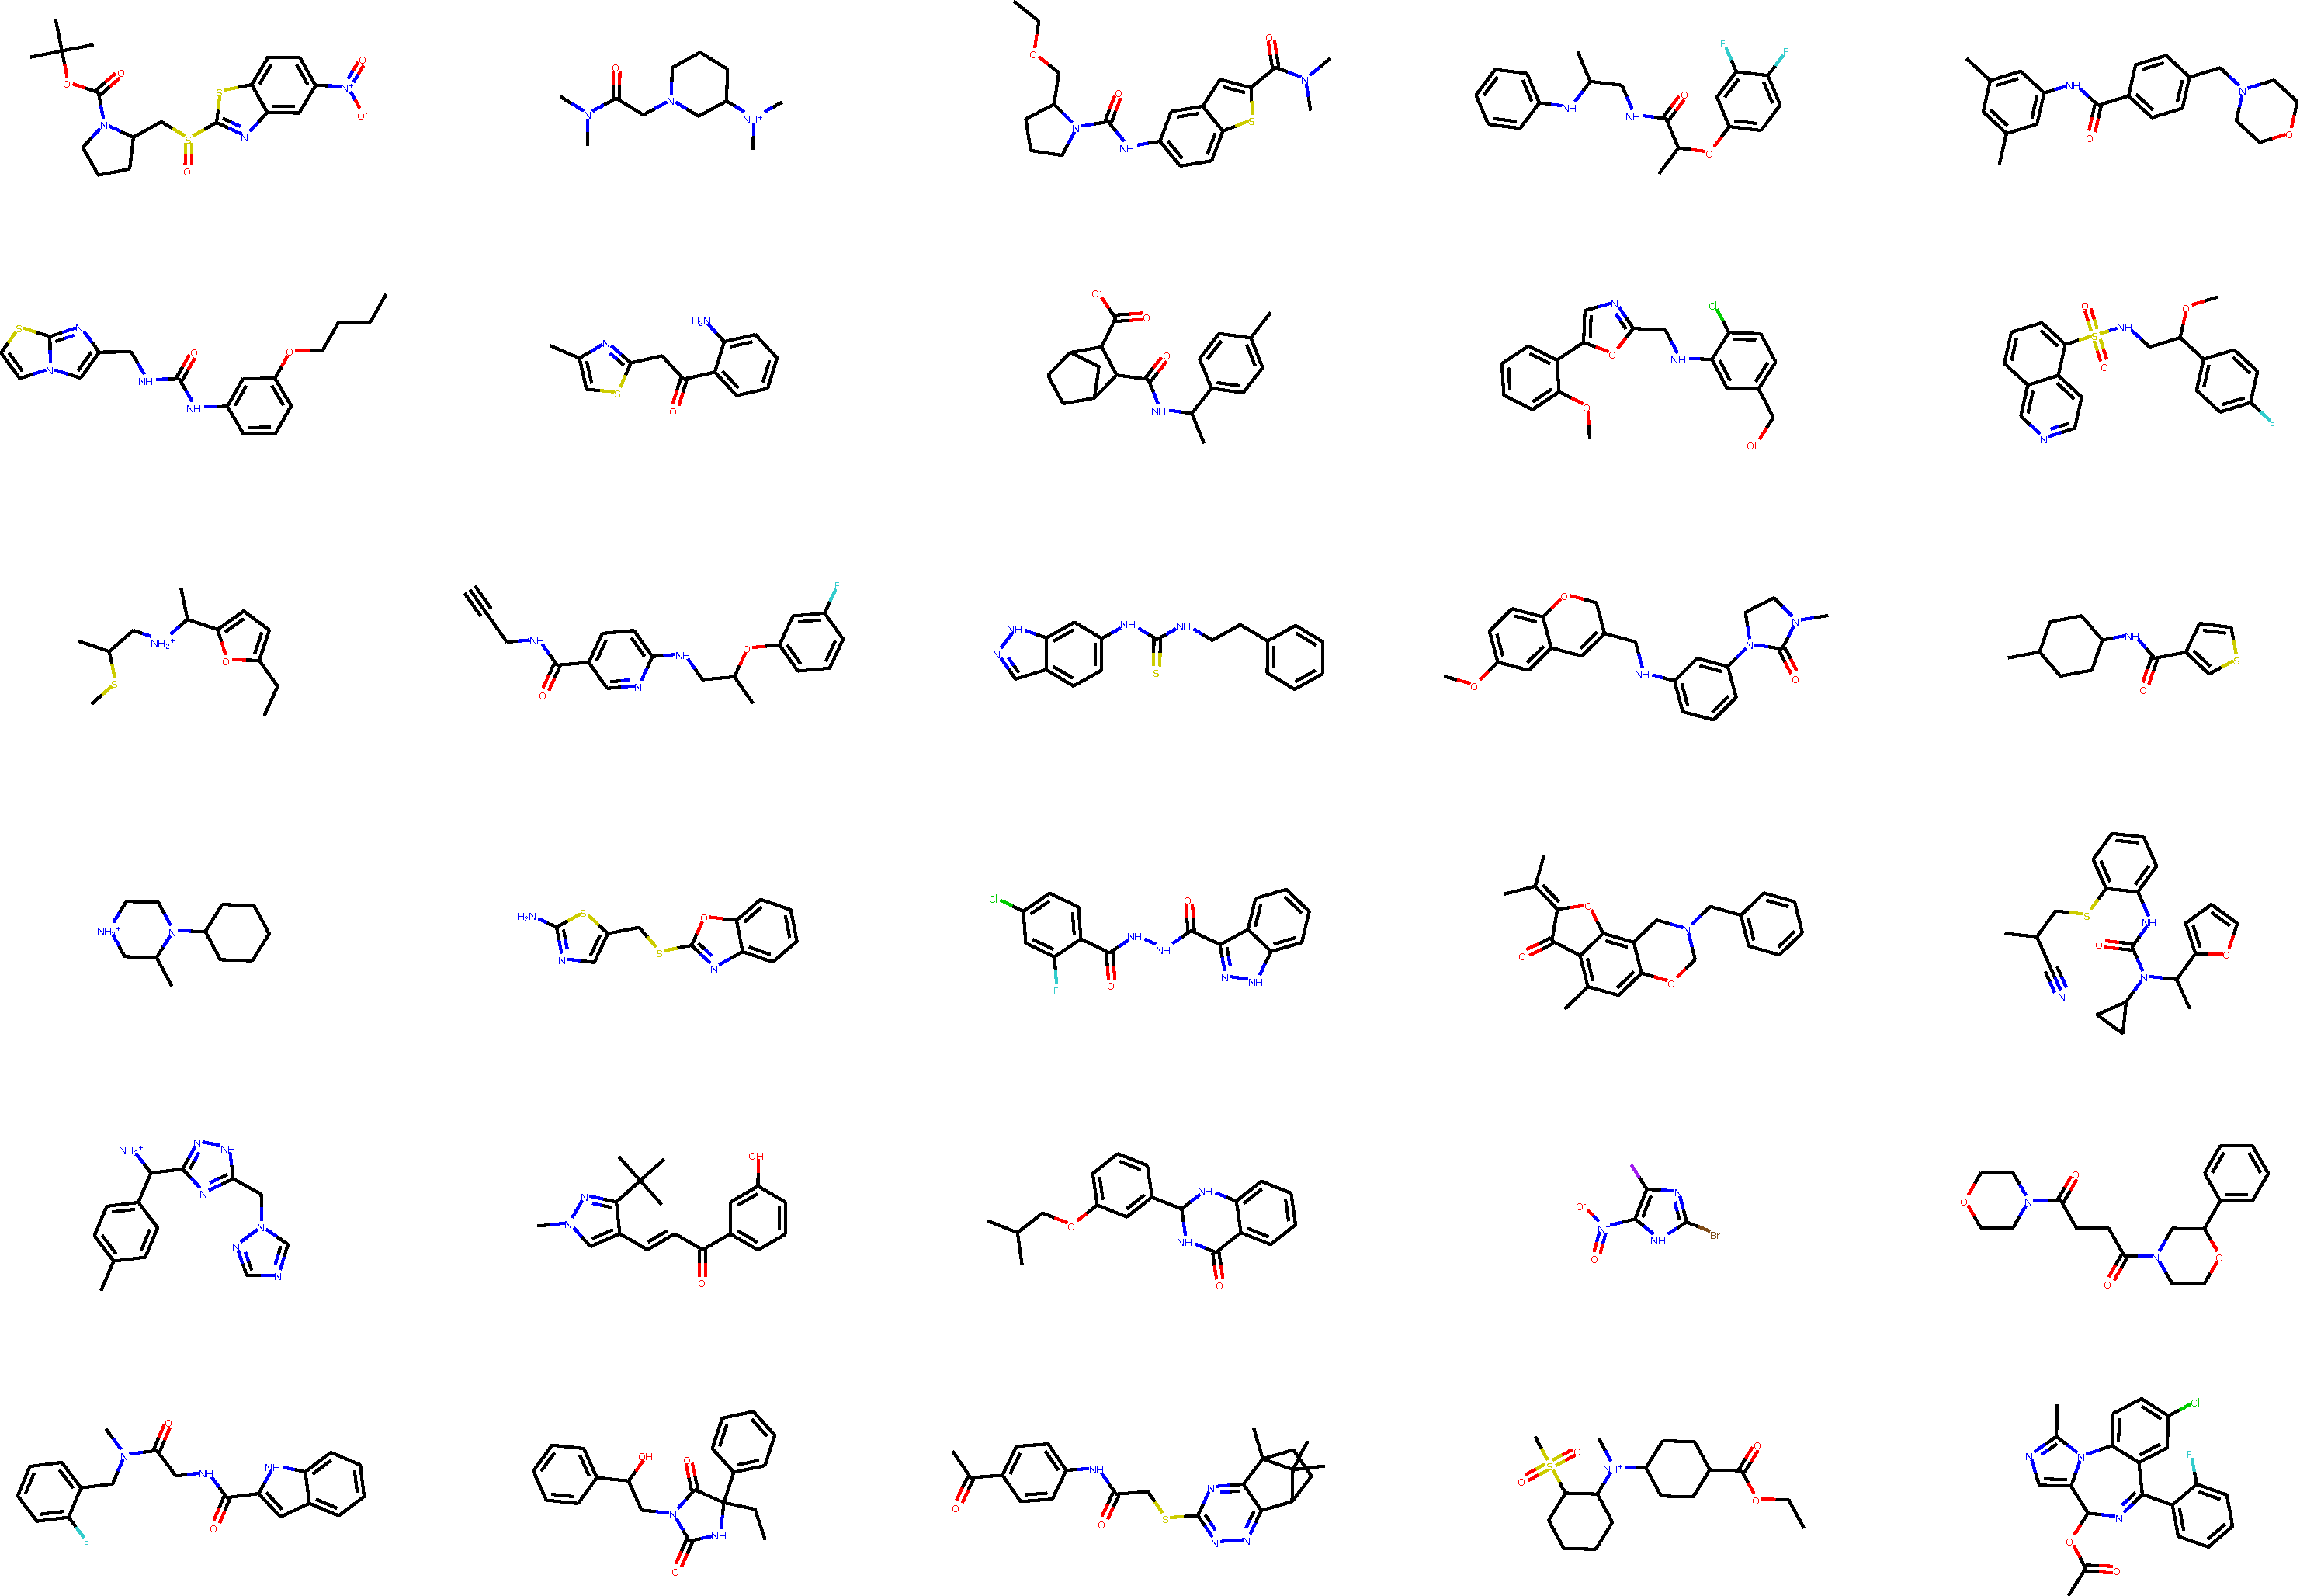
\includegraphics[width=\textwidth]{Figures/Chapter6/samples.eps}
\caption{Five randomly chosen graphs, both from the training sample (left) and generated by our model (right), on each considered dataset (displayed by row). Notice how our generative model has picked up all the characterizing connectivity patterns.}
\label{fig:samples}
\end{figure}

\subsubsection*{Effect of Node Ordering}
As we mentioned earlier, our model is strongly dependent on the type of ordering that is superimposed on graph nodes before training. To this end, we compared our model with 5 variants trained with different ordering strategies. Choices include:

\begin{itemize}
    \item a complete random strategy, which consist in randomly shuffling the node IDs before training, for each graph in the training set. This strategy is expected to perform very poorly, since the model does not see consistent connectivity patterns during training;
    \item the node ordering strategy proposed by \citet{you2018graphrnn}, which we term BF random. Such strategy is very similar to ours (in fact, our strategy is inspired by this), but differs in the fact that the starting node for the breadth-first visit of the graph is selected at random at each epoch. This in principle means that the model is trained on every possible node permutation induced by a breadth-first visit of the graph. On one hand this strategy acts as a regularizer, since at each epoch the training set changes completely. On the other hand, however, changing the node ordering at each epoch could in principle prevent our model from focusing on useful connectivity patterns, simply because they are "masked" away by different node permutations;
    \item a variant of the above mentioned BF random strategy which uses Depth-First Search (DFS) instead of BFS;
    \item only for the Enzymes and Protein datasets, a node ordering strategy induced by the SMILES encoding of the corresponding molecular graph; that is, the order of nodes is given by the position of the corresponding atom label in the SMILES string associated to the molecular graph. Notice that, even though this strategy can in principle produce canonical orderings, it is directly applicable only to molecular graphs who are annotated with atom (node) and bond (edge) labels;
    \item a variant of our proposed strategy which based on DFS.
\end{itemize}

Our first experiment consists in training the models with the alternative node ordering strategies with the same architecture as the proposed model, but trained for a large number of epochs without dropout; in short, trying to overfit the dataset on purpose. This choice is motivated by the fact that we wanted to assess whether the alternative node ordering strategies are able to memorize connectivity patterns (hence, given proper regularization, are able to generalize to unseen connectivity patterns). In Figure \ref{fig:loss}, we plot the loss obtained by the models, for each considered node ordering strategy, for the Protein dataset. The figure shows that the models trained with our strategy, the variant of our strategy based on DFS, and the SMILES ordering are able to reach a lower loss than the alternative node ordering strategies, which in contrast plateau at higher loss values. This provides evidence that our choice of node ordering strategy is well suited for our model, being sufficiently general to learn connectivity patterns from very different graph datasets. Note that the good results of the SMILES ordering was expected since our node ordering procedure resembles, although is not completely identical, to the way atoms (nodes) are ordered when deriving the SMILES string associated to the molecular graph. However, we also remark that such ordering cannot be applied in general, but it is only suitable for chemical data.

\begin{figure}[h!]
\centering
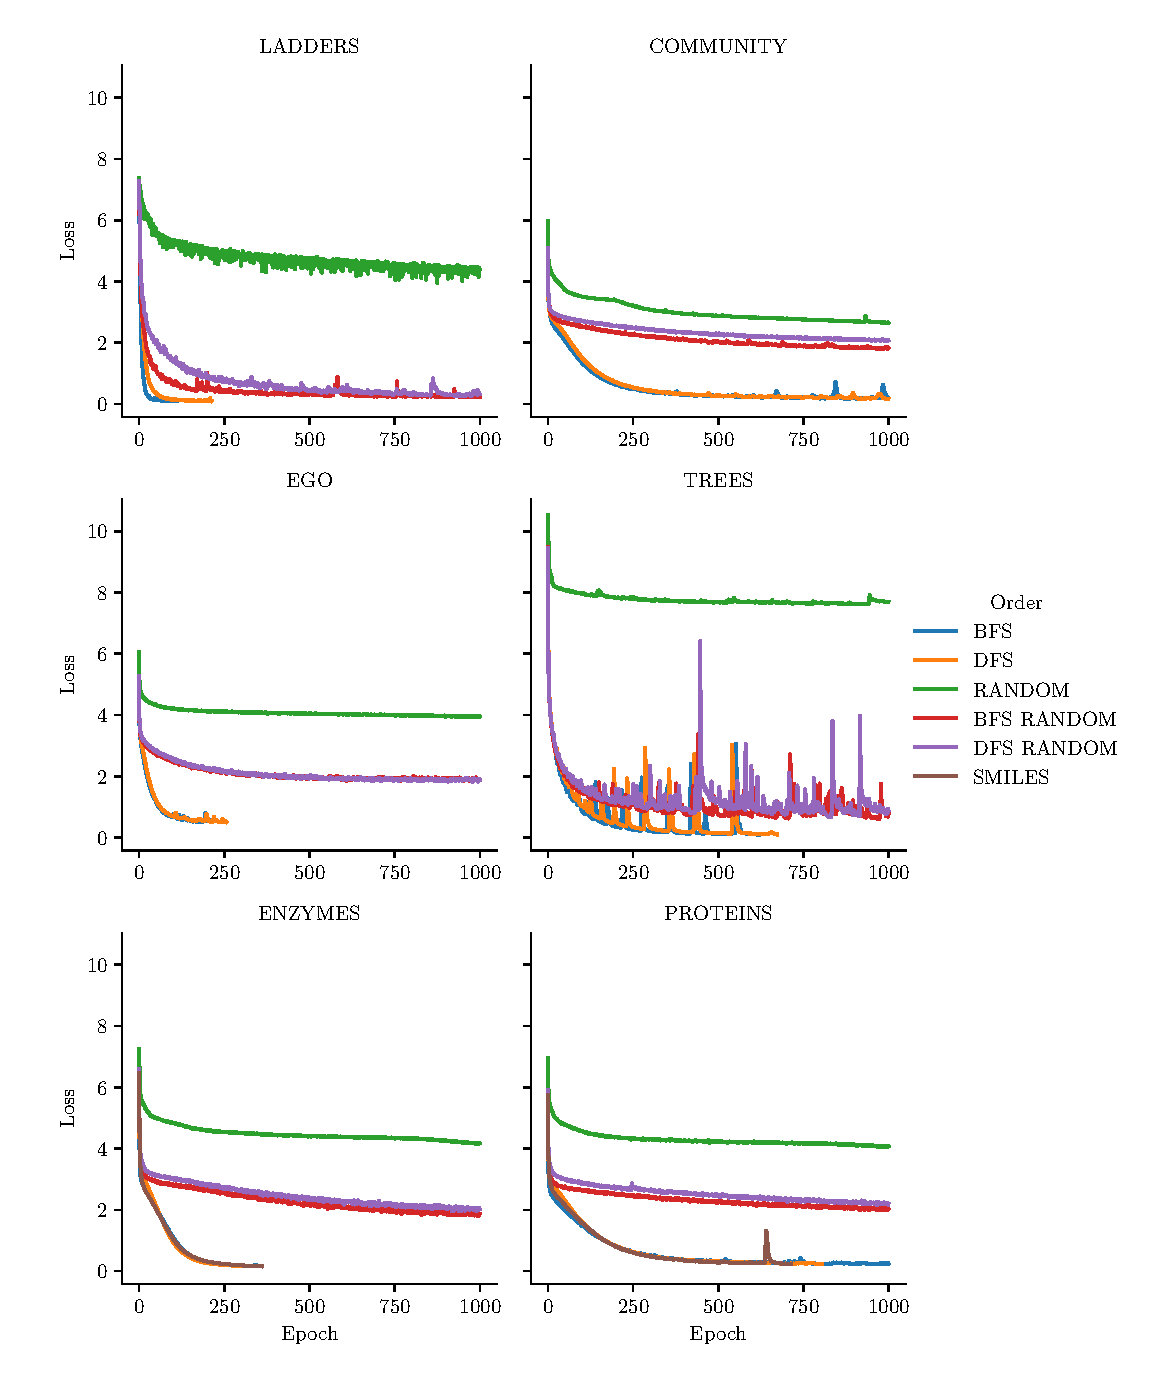
\includegraphics[width=\textwidth]{Figures/Chapter6/loss.eps}
\caption{Plot of the loss on dataset Protein of variants of our approach trained under different node orderings. Notice how the models trained with our proposed node ordering (blue), and SMILES (orange) are able to reach a lower training loss in a smaller number of epochs, compared to variants trained with random ordering (red) and BF random ordering (green).}
\label{fig:loss}
\end{figure}

We also conducted a qualitative evaluation similar to the one reported in the qualitative analysis, where we reused the results of our model and compared them to scores obtained on samples drawn from the three studied variants. Results are detailed in Table \ref{tab:graph-ordering-qualitative}, clearly showing that the model trained with our node ordering strategy is found to be superior in every chosen metric with respect to all assessed variants. The only competitive node ordering strategy is DF, which basically differs from ours in the way graph nodes are visited (DF instead of BF). However, despite being able to match the performances of our node ordering strategy in many cases, the table highlights that it may have problems in approximating structural characteristics in some dataset instances, for example the clustering coefficient in the Community dataset and the orbit count in the Ego dataset. This might be a consequence of the nature of DFS, which does not focus on local patterns first as BF does, but instead explores the graph going through sequential paths, followed by backtracking to the starting node, an approach that is probably harder to train on such datasets. In conclusion, these results further extend the evidences supporting the robustness of our approach.
\begin{table}
    \centering
    \caption{Results of the effect of node ordering on the performances of our model. The variants considered are random ordering, Breadth-First (BF) random ordering as proposed in \cite{you2018graphrnn}, SMILES ordering (only for molecular datasets), ordering of the proposed approach. Best performances are bolded.}
    \label{tab:graph-ordering-qualitative}
    \renewcommand{\arraystretch}{1.2}
    \begin{tabular}{lccccccc}
        \toprule
         \textbf{Dataset} & \textbf{Metric} & \textbf{Random} & \textbf{BFS Random} & \textbf{DFS Random} & \textbf{DFS} & \textbf{SMILES} & \textbf{Ours (BFS)}\\
         \midrule
          & ADD           & $0.643 \pm 0.094$ & $0.046 \pm 0.008$ & $0.093 \pm 0.012$ & $0.060 \pm 0.006$ & --                           & $\textbf{0.010} \pm 0.004$\\
          LADDERS & ACC   & $0.340 \pm 0.092$ & $0.031 \pm 0.012$ & $0.036 \pm 0.010$ & $\textbf{0.006} \pm 0.006$ & --                           & $\textbf{0.005} \pm 0.005$\\
          & AOC           & $2.487 \pm 0.403$ & $0.701 \pm 0.151$ & $1.125 \pm 0.145$ & $0.851 \pm 0.160$ & --                           & $\textbf{0.301} \pm 0.100$\\
         \midrule
          & ADD           & $0.038 \pm 0.004$ & $0.041 \pm 0.003$ & $0.054 \pm 0.005$ & $0.044 \pm 0.006$ & --                           & $\textbf{0.017} \pm 0.003$\\
          COMMUNITY & ACC & $1.090 \pm 0.103$ & $0.614 \pm 0.130$ & $2.496 \pm 0.403$ & $0.533 \pm 0.050$ & --                           & $\textbf{0.093} \pm 0.020$\\
          & AOC           & $0.403 \pm 0.026$ & $0.102 \pm 0.009$ & $0.186 \pm 0.019$ & $\textbf{0.054} \pm 0.008$ & --                           & $\textbf{0.054} \pm 0.017$\\
          \midrule
          & ADD           & $0.272 \pm 0.009$ & $0.114 \pm 0.009$ & $0.076 \pm 0.008$ & $0.060 \pm 0.013$ & --                           & $\textbf{0.022} \pm 0.005$\\
          EGO & ACC       & $0.506 \pm 0.034$ & $0.283 \pm 0.018$ & $0.219 \pm 0.049$ & $\textbf{0.078} \pm 0.013$ & --                           & $\textbf{0.066} \pm 0.010$\\
          & AOC           & $0.666 \pm 0.030$ & $0.616 \pm 0.035$ & $0.428 \pm 0.022$ & $0.284 \pm 0.022$ & --                           & $\textbf{0.114} \pm 0.010$\\
         \midrule
          & ADD           & $0.118 \pm 0.009$ & $0.103 \pm 0.007$ & $0.129 \pm 0.006$ & $0.028 \pm 0.003$ & $0.048 \pm 0.008$          & $\textbf{0.017} \pm 0.004$\\
          ENZYMES & ACC   & $1.067 \pm 0.275$ & $0.441 \pm 0.043$ & $0.968 \pm 0.083$ & $\textbf{0.064} \pm 0.014$ & $0.122 \pm 0.022$          & $\textbf{0.054} \pm 0.028$\\
          & AOC           & $0.550 \pm 0.053$ & $0.210 \pm 0.016$ & $0.438 \pm 0.026$ & $\textbf{0.083} \pm 0.018$ & $\textbf{0.134} \pm 0.021$ & $\textbf{0.106} \pm 0.021$\\
         \midrule
          & ADD           & $0.219 \pm 0.009$ & $0.176 \pm 0.007$ & $0.184 \pm 0.006$ & $0.010 \pm 0.011$ & $0.143 \pm 0.009$          & $\textbf{0.059} \pm 0.008$\\
          PROTEINS & ACC  & $0.817 \pm 0.058$ & $0.670 \pm 0.042$ & $0.925 \pm 0.056$ & $0.171 \pm 0.020$ & $0.402 \pm 0.040$          & $\textbf{0.064} \pm 0.017$\\
          & AOC           & $0.594 \pm 0.045$ & $0.202 \pm 0.014$ & $0.319 \pm 0.015$ & $0.069 \pm 0.010$ & $0.217 \pm 0.027$          & $\textbf{0.048} \pm 0.008$\\
         \bottomrule
    \end{tabular}
\end{table}


\subsection{Conclusions}
In this work, we have presented a novel generative model for graphs based on Recurrent Neural Networks, which is capable of generating high quality graphs from very different graph distributions. The key idea at the root of our work is to move from the domain of graphs to the one of sequences to simplify the learning task, while retaining most of the expressiveness. Our motivation to frame the generative process as learning problem on sequences is three-fold: (i) it is intuitive, (ii) it allows to work indirectly on smaller and informative portions of the exponentially large graph space, and (iii) it enables the use of the reliable and heavily optimized machinery of Recurrent Neural Networks to learn effectively.

With these ideas in mind, we developed a model which, first, orders nodes in a graph sequentially, then converts graphs into ordered sequences of edges, and finally learns these sequences using two RNNs. The first one predicts a sequence of source nodes, while the second uses the output of the first to predict all necessary endpoints to construct a novel graph. We tested our model against canonical random models from graph theory, a RNN baseline with limited expressiveness, and a state-of-the-art model on five different datasets. The evaluation was conducted on multiple levels, considering both quantitative performance measures such as novelty and uniqueness of generated graphs, as well as qualitative metrics to assess whether generated samples retain structural features of those in the training set. The results clearly show that our model performs at, and sometimes surpasses, the state of the art in the task.
We also conducted a study of how much the procedure chosen to superimpose an order on graph nodes is effective for the particular task of graph generation. More in detail, we compared with 5 variants of our model that were trained on different node orderings. Results show that with the ordering procedure of choice, the model can reach a lower training error, which is essential to learn the complex patterns needed to generate good quality graphs that resemble real-world ones.

The proposed model has also limitations. Even if it works empirically, the constraint imposed by the reliance on a specific ordering is unsatisfactory from a theoretical point of view. For this reason, one key step in future research is to study the node ordering problem more thoroughly, in order to relax and perhaps remove completely such constraint. Another limitation of our approach in its current form is the fact that it is not formulated to include node and edge labels, which are usually found in large classes of graph datasets such as molecular ones. While on one hand this limits the applicability of our approach on those domains, on the other we are also confident that extending the model to include node and edge labels might lead to improvements in generative tasks that deal with those kinds of graphs. Our belief is supported by the intuition that the ability of our model to well approximate structural features of graph distributions, coupled with a reliable mechanism to generate labels, could in perspective improve generalization, since conditioning the generative process not only on structure, but also on features, could help the model learn general connectivity patterns more reliably. This would also allow to compare our model to current molecular graph generator, and investigate the influence of domain specificity on this task.

As for other research directions, we mention the possibility to extend the model by adopting attention mechanisms \citep{bahdanau2015attention}, instead of conditioning the second network only on the last hidden state of the first. Another easily implementable extension of our approach is to model the generative process using a Variational Auto-Encoder in between the two recurrent neural networks, in order to constrain the latent space where the encoding of the first sequence is mapped to be normally distributed. This would have the advantage of cutting sampling time by approximately half, since the inference phase would only require to sample a point from latent space, and decode it using the second network. Lastly, a challenge for the near future is to test whether our approach is capable to scale to larger graphs, which would strengthen our positive results further, as well as expand its applicability to a broader class of problems.

\chapter{Fragment-Based Deep Generative Learning for Drug Discovery} % Main chapter title
\label{ch:deep-generative-learning-drug-discovery}
\part{Conclusions}\label{part:fin}
\chapter{Conclusions, Opportunities and Future Works} % Main chapter title
\label{ch:conclusions}

%----------------------------------------------------------------------------------------
%	THESIS CONTENT - APPENDICES
%----------------------------------------------------------------------------------------

\appendix % Cue to tell LaTeX that the following "chapters" are Appendices

% Include the appendices of the thesis as separate files from the Appendices folder
% Uncomment the lines as you write the Appendices

% Appendix A

\chapter{Hyper-Parameters Table} % Main appendix title

\label{AppendixA} % For referencing this appendix elsewhere, use \ref{AppendixA}
We report the grid of the hyper-parameters used in the experiments of Section \ref{sec:comparison-exp-setup}.
The hyper-parameters are the following:
\begin{itemize}
    \item \emph{layers}: number of DGN layers;
    \item \emph{convs per layer}: number of GCL layers for DGN layer;
    \item \emph{batch size}: size of the SGD minibatch;
    \item \emph{learning rate}: SGD learning rate;
    \item \emph{hidden size}: hidden state dimension of the GCL;
    \item \emph{epochs}: number of training epochs;
    \item \emph{l2}: L2 regularization parameter;
    \item \emph{dropout}: dropout rate;
    \item \emph{patience}: early stopping patience;
    \item \emph{optimizer}: type of optimizer;
    \item \emph{scheduler}: learning rate annealing scheduler;
    \item \emph{dense dim.}: output layer dimension;
    \item \emph{embed dim.}: size of the graph representation;
    \item \emph{neighborhood aggregation}: size of neighborhood aggregation.
\end{itemize}
\begin{landscape}
\tiny
\begin{tabular}{lcccccccccccccc}
\toprule
                                                            & Layers                                                       & \begin{tabular}[c]{@{}c@{}}Convs\\ per\\ layer\end{tabular} & Batch size                                                   & \begin{tabular}[c]{@{}c@{}}Learning \\ rate\end{tabular}   & \begin{tabular}[c]{@{}c@{}}Hidden \\ units\end{tabular}                                               & Epochs & L2                                                         & Dropout                                             & Patience                                                       & Optimizer & Scheduler                                                                  & \begin{tabular}[c]{@{}c@{}}Dense\\ dim\end{tabular} & \begin{tabular}[c]{@{}c@{}}Embed.\\ dim\end{tabular} & \begin{tabular}[c]{@{}c@{}}Neighbors \\ Aggregation\end{tabular}                                              \\ \midrule
\begin{tabular}[c]{@{}l@{}}Baseline\\ chemical\end{tabular} & -                                                            & -                                                            & \begin{tabular}[c]{@{}c@{}}32\\ 128\end{tabular}             & \begin{tabular}[c]{@{}c@{}}1e-1\\ 1e-3\\ 1e-6\end{tabular} & \begin{tabular}[c]{@{}c@{}}32\\ 128\\ 256\end{tabular}                                                & 5000   & \begin{tabular}[c]{@{}c@{}}1e-2\\ 1e-3\\ 1e-4\end{tabular} & -                                                   & \begin{tabular}[c]{@{}c@{}}500, loss\\ 500, acc\end{tabular}   & Adam      & -                                                                          & -                                                   & -                                                    & sum                                                      \\ \midrule
\begin{tabular}[c]{@{}l@{}}Baseline IMDB\end{tabular}   & -                                                            & -                                                            & \begin{tabular}[c]{@{}c@{}}32\\ 128\end{tabular}             & \begin{tabular}[c]{@{}c@{}}1e-1\\ 1e-3\\ 1e-6\end{tabular} & \begin{tabular}[c]{@{}c@{}}32\\ 128\\ 256\end{tabular}                                                & 3000   & \begin{tabular}[c]{@{}c@{}}1e-2\\ 1e-3\\ 1e-4\end{tabular} & -                                                   &

\begin{tabular}[c]{@{}c@{}}500, loss\\ 500, acc\end{tabular}   & Adam      & -                                                                          & -                                                   & -                                                    & sum                                                      \\ \midrule
\begin{tabular}[c]{@{}l@{}}Base. COLLAB \\ and REDDIT\end{tabular}   & -                                                            & -                                                            & \begin{tabular}[c]{@{}c@{}}32\\ 128\end{tabular}             & \begin{tabular}[c]{@{}c@{}}1e-1\\ 1e-3\end{tabular} & \begin{tabular}[c]{@{}c@{}}32\\ 128\end{tabular}                                                & 3000   & \begin{tabular}[c]{@{}c@{}}1e-2\\ 1e-3\\ 1e-4\end{tabular} & -                                                   &

\begin{tabular}[c]{@{}c@{}}500, loss\\ 500, acc\end{tabular}   & Adam      & -                                                                          & -                                                   & -                                                    & sum                                                      \\ \midrule
\begin{tabular}[c]{@{}l@{}}Baseline\\ ENZYMES\end{tabular}  & -                                                            & -                                                            & 32                                                           & \begin{tabular}[c]{@{}c@{}}1e-1\\ 1e-3\\ 1e-6\end{tabular} & \begin{tabular}[c]{@{}c@{}}32\\ 64\\ 128\\ 256\end{tabular}                                           & 5000   & \begin{tabular}[c]{@{}c@{}}1e-2\\ 1e-3\\ 1e-4\end{tabular} & -                                                   & \begin{tabular}[c]{@{}c@{}}1000, loss\\ 1000, acc\end{tabular} & Adam      & -                                                                          & -                                                   & -                                                    & sum                                                      \\ \midrule
DGCNN                                                       & \begin{tabular}[c]{@{}c@{}}2\\ 3\\ 4\end{tabular}            & 1                                                            & \begin{tabular}[c]{@{}c@{}}50 (cpu)\\ 16 (gpu)\end{tabular}  & \begin{tabular}[c]{@{}c@{}}1e-4\\ 1e-5\end{tabular}        & \begin{tabular}[c]{@{}c@{}}32\\ 64\end{tabular}                                                       & 1000   & -                                                          & 0.5                                                 & \begin{tabular}[c]{@{}c@{}}500, loss\\ 500, acc\end{tabular}   & Adam      & -                                                                          & 128                                                 & -                                                    & mean                                                    \\ \midrule
DiffPool                                                    & \begin{tabular}[c]{@{}c@{}}1\\ 2\end{tabular}                & 3                                                            & \begin{tabular}[c]{@{}c@{}}20 (cpu)\\ 8 (gpu)\end{tabular}   & \begin{tabular}[c]{@{}c@{}}1e-3\\ 1e-4\\ 1e-5\end{tabular} & \begin{tabular}[c]{@{}c@{}}32\\ 64\end{tabular}                                                       & 3000   & -                                                          & -                                                   & \begin{tabular}[c]{@{}c@{}}500, loss\\ 500, acc\end{tabular}   & Adam      & -                                                                          & 50                                                  & \begin{tabular}[c]{@{}c@{}}64\\ 128\end{tabular}     & mean                                                      \\ \midrule
ECC                                                         & \begin{tabular}[c]{@{}c@{}}1\\ 2\end{tabular}                & 3                                                            & \begin{tabular}[c]{@{}c@{}}32 (cpu)\\ 8 (gpu)\end{tabular}   & \begin{tabular}[c]{@{}c@{}}1e-1\\ 1e-2\end{tabular}        & \begin{tabular}[c]{@{}c@{}}32\\ 64\end{tabular}                                                       & 1000   & -                                                          & \begin{tabular}[c]{@{}c@{}}0.05\\ 0.25\end{tabular} & \begin{tabular}[c]{@{}c@{}}500, loss\\ 500, acc\end{tabular}   & SGD       & ECC-LR                                                                     & -                                                   & -                                                    & sum                                                      \\ \midrule
GIN                                                         & \begin{tabular}[c]{@{}c@{}}see\\ hidden\\ units\end{tabular} & 1                                                            & \begin{tabular}[c]{@{}c@{}}32\\ 128\end{tabular}             & 1e-2                                                       & \begin{tabular}[c]{@{}c@{}}32 (5 layers)\\ 64 (5 layers)\\ 64 (2 layers)\\ 32 (3 layers)\end{tabular} & 1000   & -                                                          & \begin{tabular}[c]{@{}c@{}}0\\ 0.5\end{tabular}     & \begin{tabular}[c]{@{}c@{}}500, loss\\ 500, acc\end{tabular}   & Adam      & \begin{tabular}[c]{@{}c@{}}Step-LR\\ (step: 50,\\ gamma: 0.5)\end{tabular} & -                                                   & -                                                    & sum                                                      \\ \midrule
GraphSAGE                                                   & \begin{tabular}[c]{@{}c@{}}3\\ 5\end{tabular}                & 1                                                            & \begin{tabular}[c]{@{}c@{}}32 (cpu)\\ 16 (cuda)\end{tabular} & \begin{tabular}[c]{@{}c@{}}1e-2\\ 1e-3\\ 1e-4\end{tabular} & \begin{tabular}[c]{@{}c@{}}32\\ 64\end{tabular}                                                       & 1000   & -                                                          & -                                                   & \begin{tabular}[c]{@{}c@{}}500, loss\\ 500, acc\end{tabular}   & Adam      & -                                                                          & -                                                   & -                                                    & \begin{tabular}[c]{@{}c@{}}mean\\ max\\ sum\end{tabular} \\
\bottomrule
\end{tabular}
\end{landscape}

\afterpage{\blankpage}

\chapter{List of Publications}\label{AppendixB}

\begin{itemize}
\item F. Errica, M. Podda, D. Bacciu, A. Micheli. "A Fair Comparison of Graph Neural Networks for Graph Classification".
\textit{8th International Conference on Learning Representations (ICLR)}. (2020)
\item M. Podda, D. Bacciu, A. Micheli. "A Deep Generative Model for Fragment-Based Molecule Generation". \textit{Proceedings of the Twenty Third International Conference on Artificial Intelligence and Statistics (AISTATS)}. Vol. 108, pages 2240-2250. (2020)
\item D. Bacciu, F. Errica, A. Micheli, M. Podda. "A Gentle Introduction to Deep Learning for Graphs". \textit{Neural Networks}. Volume 129, Pages 203-221. ISSN 0893-6080, doi:10.1016/j.neunet.2020.06.006. (2020)
\item P. Bove, P. Milazzo, A. Micheli, M. Podda.
"Prediction of dynamical properties of biochemical pathways with Graph Neural Networks". \textit{Proceedings of the 13th International Joint Conference on Biomedical Engineering Systems and Technologies - Volume 3: BIOINFORMATICS}. ISBN 978-989-758-398-8, pages 32-43. doi:10.5220/0008964700320043 (2020)
\item M. Podda, D. Bacciu, A. Micheli, P. Milazzo. "Biochemical Pathway Robustness Prediction with Graph Neural Networks". \textit{To appear in: ESANN 2020 Proceedings} (2020)
\item D. Bacciu, A. Micheli, M. Podda. "Edge-based sequential graph generation with recurrent neural networks". \textit{Neurocomputing},
Volume 416, pages 177-189, ISSN 0925-2312. doi:10.1016/j.neucom.2019.11.112. (2020)
\item D. Bacciu, A. Micheli, M. Podda. "Graph generation by sequential edge prediction". \textit{ESANN 2019 Proceedings}, pages 95-100, ISBN 978-287-587-065-0. (2019)
\item M. Podda, D. Bacciu, A. Micheli, R. Bellù, G. Placidi, L. Gagliardi. "A machine learning approach to estimating preterm infants survival: development of the Preterm Infants Survival Assessment (PISA) predictor". \textit{Sci Rep} 8, 13743. doi:10.1038/s41598-018-31920-6 (2018)
\end{itemize}
\chapter{Contributed Code}\label{AppendixC}

\begin{itemize}
    \item Code for the article: M. Podda, D. Bacciu, A. Micheli, R. Bellù, G. Placidi, L. Gagliardi. "A machine learning approach to estimating preterm infants survival: development of the Preterm Infants Survival Assessment (PISA) predictor". \textit{Sci Rep} 8, 13743. doi:10.1038/s41598-018-31920-6 (2018)\\
    URL: \url{https://github.com/marcopodda/inn}
    \item Code for the article: D. Bacciu, A. Micheli, M. Podda. "Edge-based sequential graph generation with recurrent neural networks". \textit{Neurocomputing},
    Volume 416, pages 177-189, ISSN 0925-2312. doi:10.1016/j.neucom.2019.11.112. (2020)\\
    URL: \url{https://github.com/marcopodda/grapher}
    \item Code for the conference paper: M. Podda, D. Bacciu, A. Micheli. "A Deep Generative Model for Fragment-Based Molecule Generation". \textit{Proceedings of the Twenty Third International Conference on Artificial Intelligence and Statistics (AISTATS)}. Vol. 108, pages 2240-2250. (2020)\\
    URL: \url{https://github.com/marcopodda/fragment-based-dgm}
    \item Code for the conference paper: F. Errica, M. Podda, D. Bacciu, A. Micheli. "A Fair Comparison of Graph Neural Networks for Graph Classification".
    \textit{8th International Conference on Learning Representations (ICLR)}. (2020)\\
    URL: \url{https://github.com/diningphil/gnn-comparison}
\end{itemize}

%----------------------------------------------------------------------------------------
%	BIBLIOGRAPHY
%----------------------------------------------------------------------------------------

\printbibliography[heading=bibintoc]

%----------------------------------------------------------------------------------------

\end{document}
